\chapter{Crystallography}

\section{Lattices and Cells}

\subsection{Crystal Lattices}

A crystal is defined by the infinite, three-dimensional repetition of a structural motif. 
The underlying periodicity is described by a \emph{lattice}, an infinite array of mathematical points, each with identical surroundings. 
One lattice point stands for one structural motif.\\ \\
%
The lattice can be spanned by three linear independent vectors $\mathbf{a},\, \mathbf{b},\, \mathbf{c}$ that define the crystal axes, 
or six parameters: the repetition distance $a,\, b,\, c$ on three axes, and the angle $\alpha,\, \beta,\, \gamma$ between the axes. 
Every point in the lattice can then be expressed in coordinate forms with integer coefficients for the three basis vectors:
%
\[
	\text{Points in the Lattice } 
	\Leftrightarrow 
	P=\{\mathbf{v}\,|\,\mathbf{v}=x\mathbf{a}+y\mathbf{b}+z\mathbf{c},\ x,y,z\in\mathbb{Z}\}
\]
%
A set of parallel, equally spaced planes that intercept the crystal axes at minimum $(a/h, b/k, c/l)$ 
is indexed by the integers $(hkl)$, known as the \emph{Miller indices}. 
If the indices are negative, we add a bar on top of that number, representing a negative sign.\\ \\
%
The distance between a set of lattice planes $(h_i)_{i=1}^{3}$ in a lattice defined by $\{a_i,\alpha_i\}_{i=1}^{3}$ is given by:
%
\[
	d^{-2} = \frac{1}{V^2} \sum( S_i h_i ^ 2 + 2 R_i h_j h_k )
\]
%
where the coefficients are defined as follows:
%
\[
	S_i=a_ja_k\sin^2\alpha_i,\ \ 
	R_i=a_i^2a_ja_k(\cos\alpha_j\cos\alpha_k-\cos\alpha_i),\ \ 
	i,j,k\in\{1,2,3\},\ i\neq j\neq k
\]
%
A family of symmetrically equivalent planes is denoted by curly braces $\{hkl\}$. 
For example, cutting a largest octahedron out of a cubic cell, then its six faces can be denoted as $\{111\}$.
Crystal directions are specified by the miller indices of the vector's fractional coordinate form, written as $[uvw]$. 
A family of symmetrically equivalent directions is denoted $\langle uvw\rangle$.
%
\subsection{Crystallographic Point Groups}
%
Because the lattice possesses translational symmetry, at least along integer multiples of the three basis vectors, 
rotational symmetry must be compatible with this periodicity that after rotation, 
the points should still land on a lattice point with integer coordinates, 
i.e. point set $P$ is close to the rotational matrix $R$, which requires its trace to be an integer.\\ \\
%
Assume the rotational axis is perpendicular to the plan spanned by two of the basis vectors, 
and in fact that's often the criterion for defining crystal axes. 
Bacause trace is invariant of coordinate selection, we can simply do the calculation in a 2 dimensional orthonormal basis.
Under this condition, the trace of matrix for rotating $\theta$ is:
%
\[
	\Tr\mathbf{R} = \Tr
	\begin{pmatrix}
		\cos\theta	&	-\sin\theta	\\
		\sin\theta	&	 \cos\theta
	\end{pmatrix} = 
	2\cos\theta\in\mathbb{Z}
\]
%
Therefore for $\theta$ to be the factor of $2\pi$:
\[
	\theta=\frac{2\pi}{n} 
	\quad\Rightarrow\quad 
	n\in\{1,2,3,4,6\}
\]
%
Which means crystallographic point groups can only have 1,2,3,4,6-fold rotational axes.
%
\subsubsection{Hermann-Mauguin Symbols}
%
In crystallography, we use Hermann-Mauguin symbols instead of Scheonflies symbols for symmetry operations, 
and point groups are denoted with essential symmetry operations along 
(or perpendicular for mirror planes) the three crystal axes. 
The rules are listed in table \ref{convert}:
%
\begin{table}
	\centering
	\begin{tabular}{@{}ll@{}}
		\toprule
		\ \textbf{Hermann-Mauguin} 	& \textbf{Scheonflies}\ 	\\
		\midrule
		\ $n$ 						& $C_n$						\\
		\ $\bar{n}$ 				& $I_n$						\\
		\ $m$ or $\bar{2}$ 			& $\sigma$					\\
		\ $\bar{1}$ 				& $i$						\\
	\bottomrule
	\end{tabular}
	\caption{Conversion between Hermann-Mauguin and Scheonflies symbols}
	\label{convert}
\end{table}
%
For example, $6/mmm$ denotes there is a six-fold rotational axes along the first direction 
and a mirror plane perpendicular to the axis, and one mirror plane perpendicular to each other two directions.
%
\subsection{Crystal Cells}
To better understand a infinite lattice, we concentrate on one fraction of it called a cell, 
a parallelepiped that can reconstruct the whole lattice by translating itself by $\mathbf{v}\in P$.
Points in a cell can be located using fractional coordinates $(x, y, z)$ located at:
%
\[
	\mathbf{r}=x\mathbf{a}+y\mathbf{b}+z\mathbf{c},\ \ 
	x,y,z\in[0,1)
\]
%
The volume of an arbitrary cell can be calculated from its parameters:
\[
	V=abc\sqrt{1-\cos^2\alpha-\cos^2\beta-\cos^2\gamma+2\cos\alpha\cos\beta\cos\gamma}
\]
%
\subsubsection{Counting Lattice Points}
%
\begin{table}
	\centering
	\begin{tabular}{@{}lll@{}}
		\toprule
		\ \textbf{Position}	& \textbf{Shared by}	& \textbf{Point Count}\ 	\\
		\midrule
		\ Vertex			& 8						& 1/8						\\
		\ Edge				& 4						& 1/4						\\
		\ Face				& 2						& 1/2						\\
		\ Inside			& 1 					& 1							\\
		\bottomrule
	\end{tabular}
	\caption{Lattice Point Count in Cells}
\end{table}
%
A primitive cell contains only one lattice point (structural motif) 
usually at its eight vertices, other conventional cells can have centerings:
%
\begin{table}
	\centering
	\begin{tabular}{@{}llll@{}}
		\toprule
		\ \textbf{Centering}	& \textbf{Symbol}	& \textbf{Extra lattice points}				& \textbf{Extra Translational Symmetry}\ 	\\
		\midrule
		\ Primitive				& $P$				& None                          			& None										\\
		\ Body-centered			& $I$             	& $(1/2,\ 1/2,\ 1/2)$						& $(\mathbf{a}+\mathbf{b}+\mathbf{c})/2$\	\\
		\ Face-centered			& $F$             	& $(1/2,\ 0,\ 1/2)$ (circulant)				& $(\mathbf{a}+\mathbf{c})/2$ (circulant)\	\\
		\ Base-centered			& $C$ usually		& $(1/2,\ 1/2,\ 0)$							& $(\mathbf{a}+\mathbf{b})/2$ 				\\
		\ Rombohedral			& $R$			 	& $(1/3,\ 2/3,\ 2/3)$, $(2/3,\ 1/3,\ 1/3)$	& $(\mathbf{a}+\mathbf{b}+\mathbf{c})/3$\	\\
		\bottomrule
	\end{tabular}
	\caption{Lattice Types}
\end{table}
%
For one lattice, there're infinite many valid cells, but its usually taken by the following criteria:
%
\begin{itemize}
	\item Validity: satisfies translational symmetry (top priority);
	\item Symmetry: fully exhibits the symmetry of the lattice;
	\item Angle: Obtuse better than acute, $\pi/2$ and $2\pi/3$ preferred;
	\item Size: As small as possible.
\end{itemize}
%
A cell satisfying these requirements is called a unit cell. 
It contains the minimal information required to describe the whole crystal structure.
%
\subsection{Crystal Systems and Bravis Lattices}
%
According to the symmetry of lattices, 
14 kinds of lattices belonging to 7 crystal systems are classified in figure \ref{bravis}.
%
\begin{figure}[h]
	\centering
	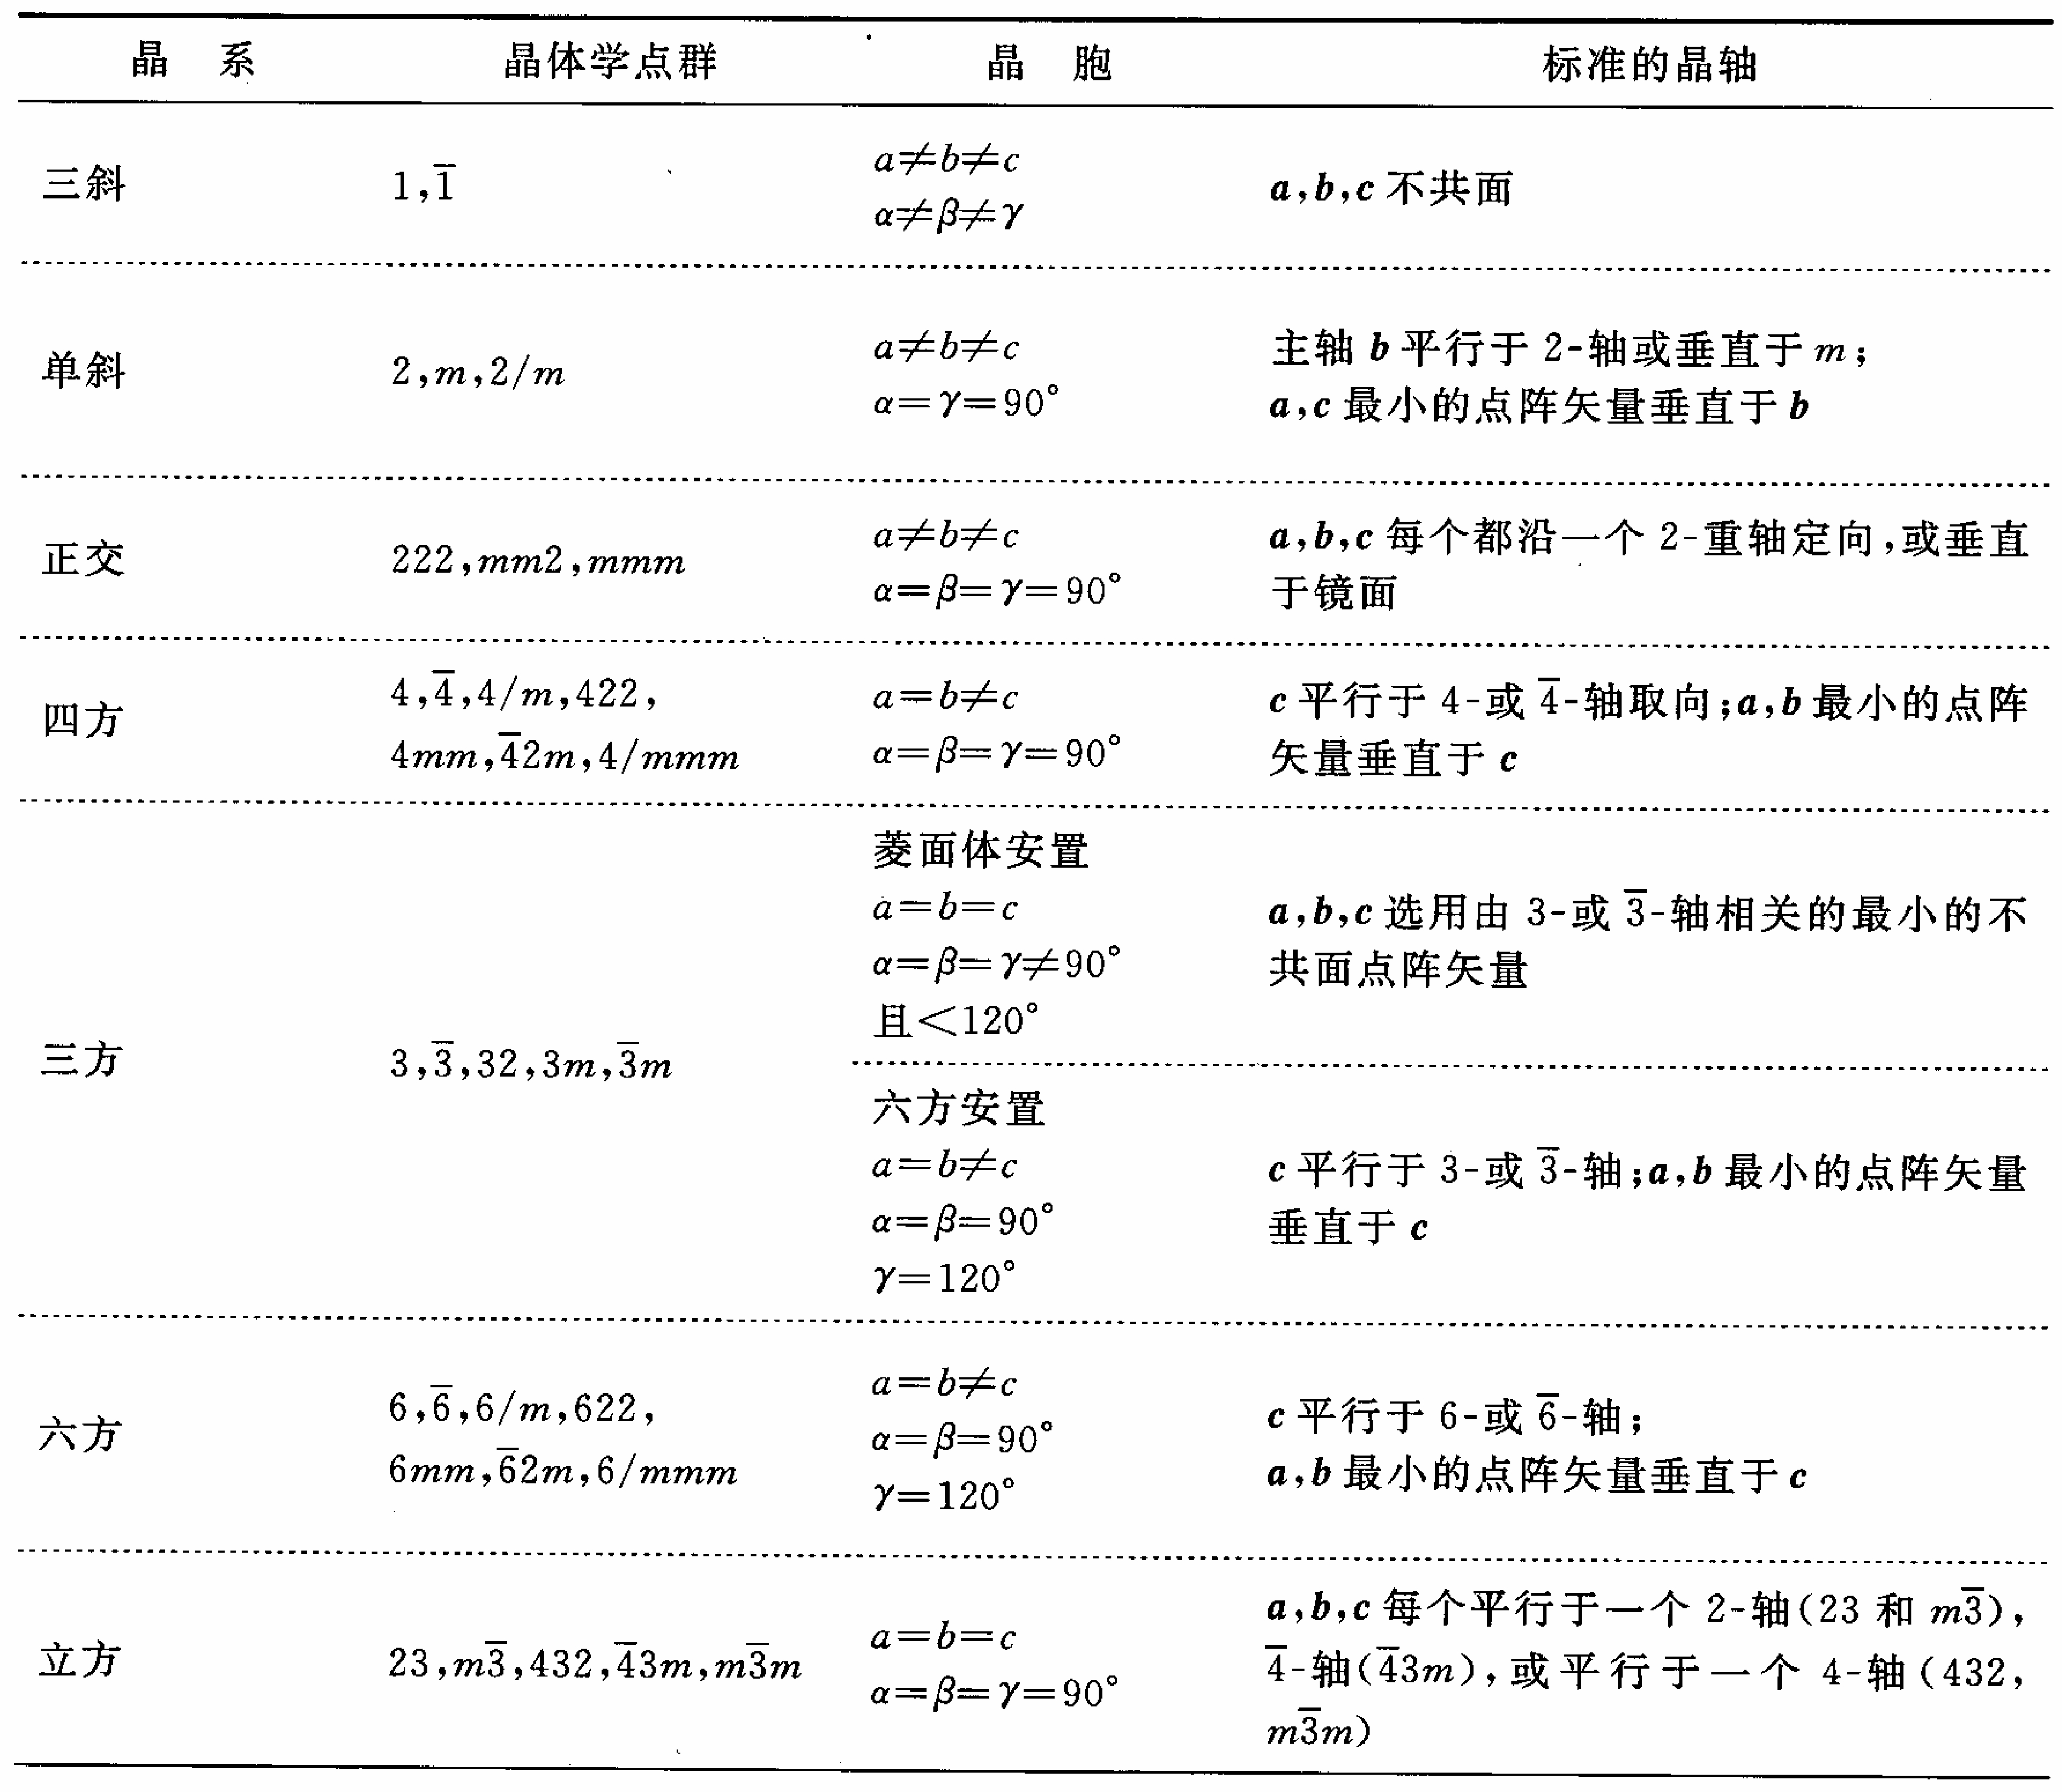
\includegraphics[scale=0.1]{Ch10/Lattice/bravis}
	\caption{7 Bravis Crystal Systems}
	\label{bravis}
\end{figure}
%
The 14 Bravis lattices are then: 
\[
	aP,\ mP,\ mC,\ oP,\ oC,\ oI,\ oF,\ hP,\ hR,\ tP,\ tI,\ cP,\ cI,\ cF
\]
%
\subsection{Translational Symmetry and Space Groups}
%
A \emph{space group} is the complete set of symmetry operations that leave a crystal structure invariant. 
It combines the point-group operations (proper/improper rotations) with the translational symmetry of the Bravais lattice, 
and introduces \emph{new} operations that are products of point operations and fractional translations.
Because translations are involved, the order of operations matters. 
The full 3D space-group symbols (Hermann--Mauguin notation) have the general form:
%
\[\rm
	Lattice\ type + symmetry\ along\ principal\ axis + symmetry\ along\ secondary\ axes
\]
%
\subsubsection{Screw Axes and Glide Planes}
%
A \emph{screw axis} $n_m$ denotes an $n$-fold rotation followed by a translation of $m/n$ of the unit-cell length along the axis.
A \emph{glide plane} combines reflection with a translation parallel to the plane by half a lattice vector. 
The notation indicates the direction of the glide:
%
\begin{itemize}
    \item $a$, $b$, $c$: glide along the respective axis.
    \item $n$: diagonal glide (e.g., translation $(\mathbf{a}+\mathbf{b})/2$).
    \item $d$: diamond glide (translation $(\mathbf{a}\pm\mathbf{b})/4$ etc.), found only in face- or body-centered lattices.
\end{itemize}
%
\subsubsection{Space Group Notation}
%
The first symbol gives the Bravais-lattice type ($P,A,B,C,I,F,R$). 
The subsequent entries give the principal symmetry operators in order of decreasing symmetry. 
Detailed rules are given in figure \ref{spacegroup}
%
\begin{figure}[h]
	\centering
	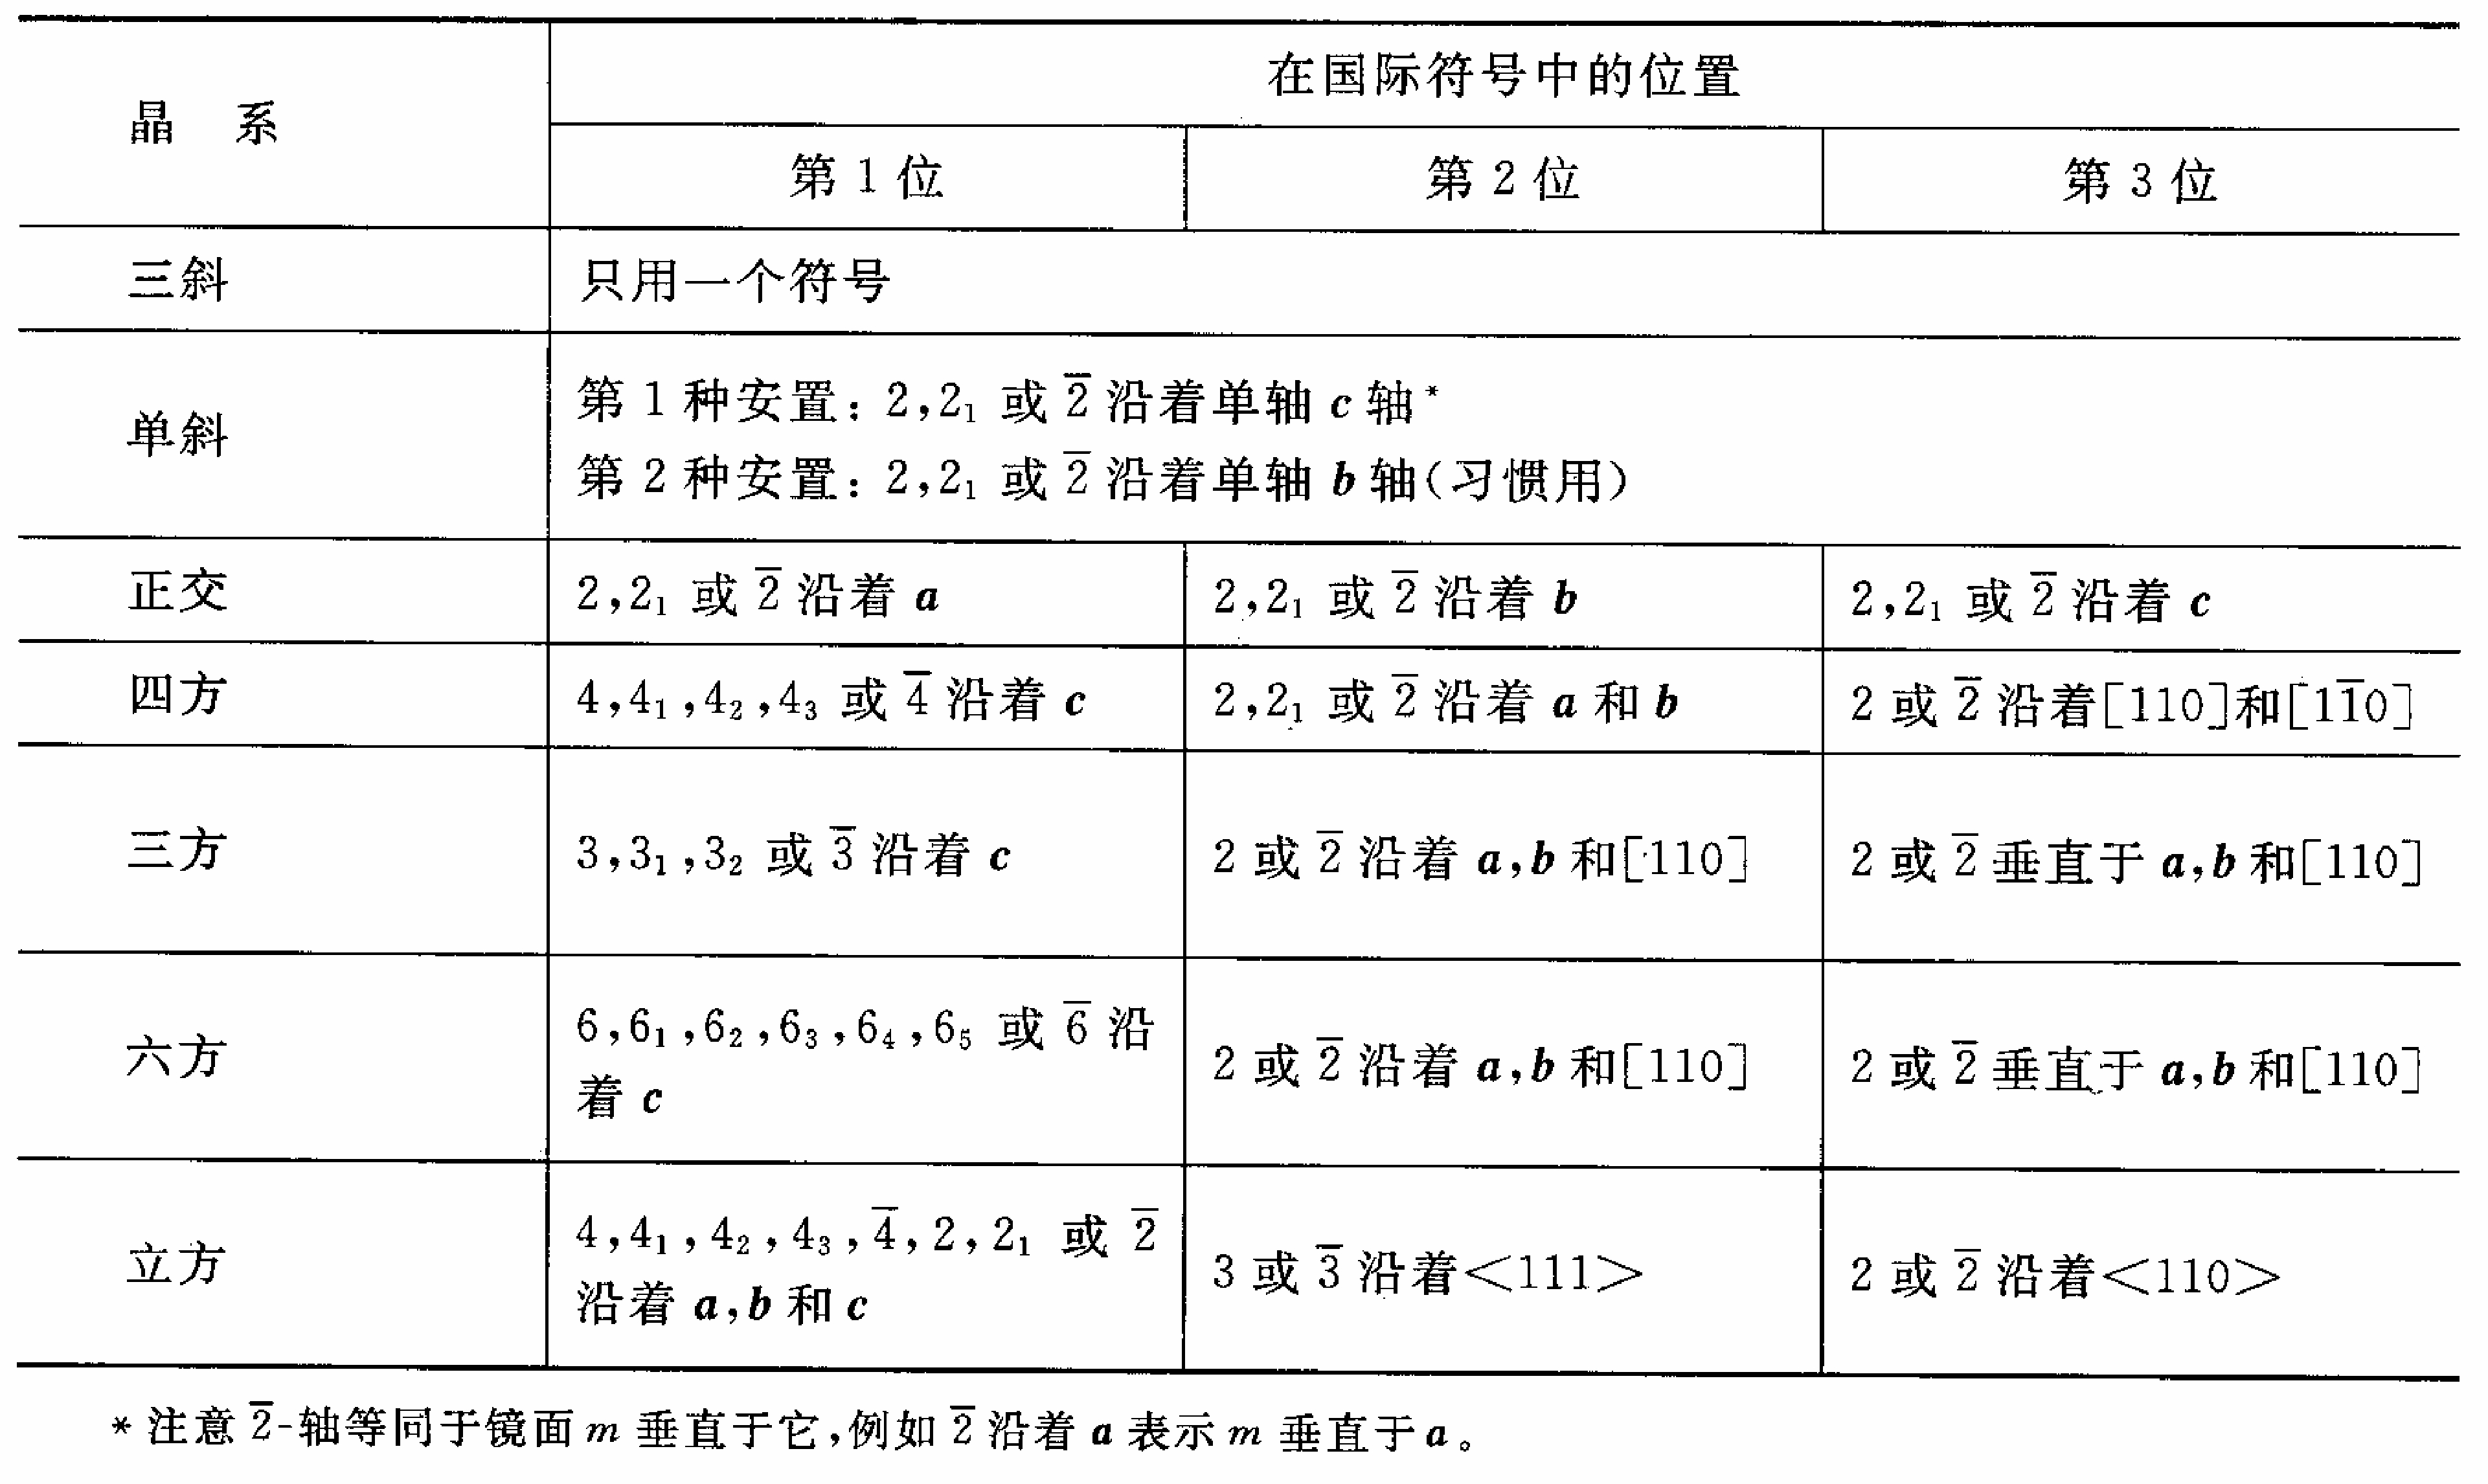
\includegraphics[scale=0.1]{Ch10/Lattice/spacegroup}
	\caption{Order of symmetry operations in space group notation}
	\label{spacegroup}
\end{figure}
%
There are 230 distinct space groups in three dimensions.
%
\subsection{Determination of Space Groups via X-Ray Diffraction}
%
\subsubsection{Bragg's Law}
%
When the size of an obstacle in the way of electromagnetic waves is comparable to the wavelength, 
different waves passing through the obstacle will interfere due to path difference, which phenomenon is named diffraction.\\ \\
%
Consider lattice planes as semi-transparent mirrors, constructive interference occurrs 
when the path difference between waves reflected from adjacent planes is an integer multiple of the wavelength, 
showing an enhanced intensity on the screen which is described as a reflection.\\ \\
%
By experimental convention, a incident beam of monochromatic X-ray with wavelength $\lambda$ 
enters the crystal at an angle $\theta$ ranging between $(0, \pi/2]$, 
then for a reflection by a set of lattice planes with distance $d$ to occur, the incident angle must satisfy:
%
\[
	2d\sin\theta=n\lambda
\]
%
where $n$ is the order of reflection. 
By redefining the reflecting planes as $(nh,nk,nl)$, 
one may absorb $n$ into the Miller indices and write the first-order law for any set of planes.\\ \\
For a cubic crystal, the Bragg condition becomes:
%
\[
	\sin\theta = \frac{(h^2+k^2+l^2)^{1/2}\lambda}{2a}.
\]
%
Because $h^2+k^2+l^2$ cannot equal certain integers (e.g., 7, 15, 23, 28, 31, \dots), 
these systematic absences are characteristic signatures of specific lattice types 
(e.g., the primitive cubic lattice shows no reflection when the sum is 7).
%
\subsubsection{Structure Factor}
%
It's a bit radical to treat lattice planes as semi-transparent mirrors, 
since it is the atoms' electrons that scatters the incident wave. 
We introduce the atomic scattering factor to measure the amplitude of atomic scattering wave compared with a single electron:
%
\[
	f(\theta)=4\pi\int_{0}^{\infty}\rho(r)\frac{\sin kr}{kr}r^2\df r,\quad k=\frac{4\pi}{\lambda}\sin\theta
\]
%
where $\rho(r)$ is the radial electron density and $4\pi r^2\df r$ is a spherical shell volume differential.
In the forward direction ($\theta = 0$), we have
%
\[
\lim_{kr\to 0}\,\frac{\sin kr}{kr}=1, \ \ \Rightarrow\ \ 
f(0) = 4\pi\int_0^\infty \rho(r)r^2\,\mathrm{d}r = Z,
\]
%
Thus, the forward scattering factor equals the total number of electrons.\\ \\
%
Consider an atom placed on fractional position $x\in[0,1)$ between two adjacent $(100)$ planes.
When first order reflection occurrs, i.e. phase difference between the scattering wave from two planes is $2\pi$, 
the phase difference between scattering waves from the atom and from the planes is then $2x\pi$. Note that as $x$ can be 0, 
the reflection by the planes has already been taken into account.\\ \\
%
Generalizing it to an arbitrary cell with atoms at fractional coordinates $(x_i,y_i,z_i)$ with scattering factor $f_j$.
At the angle of plane $(hkl)$ reflection, the atomic scattering wave is different in phase to waves scattered by the planes by:
%
\[
	\phi_i^{hkl} = 2\pi(hx_i+ky_i+lz_i)
\]
%
Therefore the total amplitude of reflection by $(hkl)$ is the sum of all atomic scattering waves (amplitude $\times$ phase), 
namely the structure factor, and the intensity is proprotional to its modulo square.
%
\[
	F_{hkl} = \sum_i f_i\,\exp\left(i\phi_i^{hkl}\right) = \sum_i f_i\,\exp\left[2\pi i(hx_i+ky_i+lz_i)\right]
\]
%
If the phase difference given by atoms is an odd multiple of $\pi$, i.e. $2(hx_i+ky_i+lz_i)=2m+1,\,m\in\mathbb{Z}$, 
destructive inteference occurrs giving diminished reflection. 
Those diminished reflection caused by the symmetry and type of cells are named systematic absences, 
which helps to determine centerings and symmetry elements of cells:
%
\begin{itemize}
	\item Body-centered: Atoms at $(0,\,0,\,0)$ and $(1/2,\,1/2,\,1/2)$ give a phase difference of $(h+k+l)\pi$. 
			Thus, reflections with $h+k+l$ odd are absent.
	\item Face-centered: Reflections are present only when $h,k,l$ are either all even or all odd.
	\item Screw axes / Glide planes: A $2_1$ screw along $c$ extinguishes $00l$ when $l$ is odd; 
			a $c$ glide perpendicular to $b$ extinguishes $h0l$ when $l$ is odd, etc.
\end{itemize}
%
These extinctions are the experimental signature used to determine the space group.\\ \\
%
Because diffractometers measure structure factors, electron densities can be reconstructed via inverse Fourier transform, 
so called the Fourier synthesis of electron density:
%
\[
	\rho(\mathbf{r}) = \frac{1}{V}\sum_{hkl} F_{hkl}\,\exp\left[-2\pi i(hx+ky+lz)\right]
\]
%
where $V$ is the unit-cell volume. This is the fundamental link between diffraction data and structure.
%
\section{Closest-Packing Patterns}
%
\subsection{Two-Layer Closest Packing}\ \\ \\
%
When packing one layer of hard spheres as dense as possible, the best strategy is having every sphere tangent with another six, 
forming a hexagonal pattern as shown in figure \ref{closestpack_1}. 
This creates two kinds of triangular interstices: 
the $\Delta$ interstice, denoted by $\times$ in the figure, and the $\nabla$ interstice, denoted by $\circ$.\\
%
\begin{figure}[h]
	\centering
	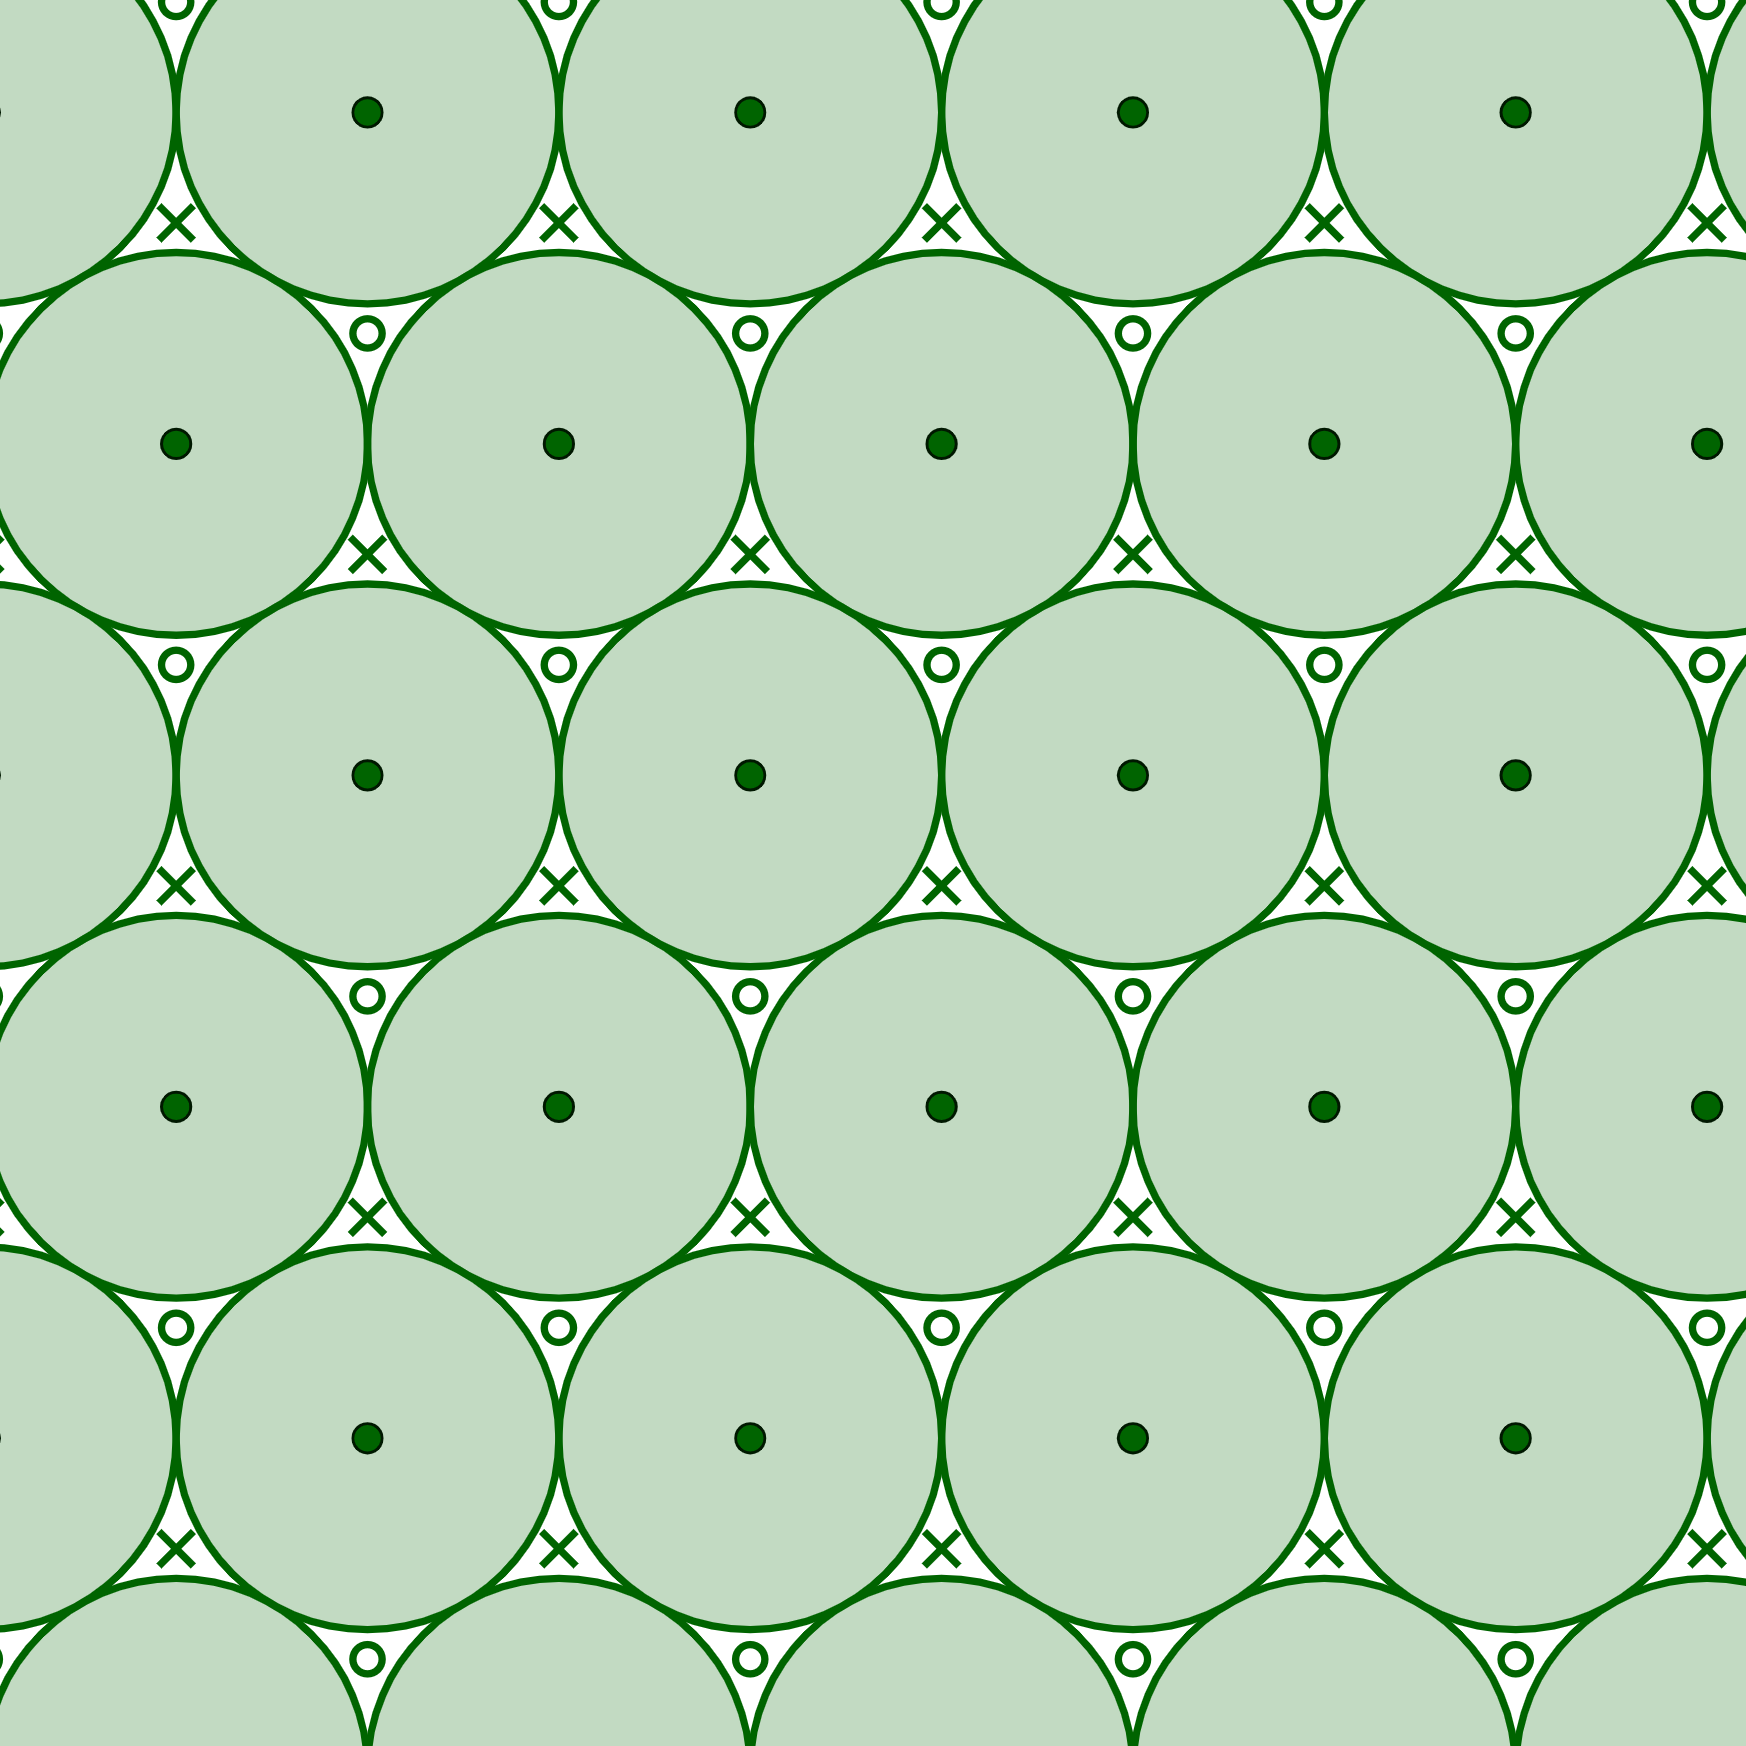
\includegraphics[scale=1]{Ch10/ClosestPacking/ClosestPacking1}
	\quad
	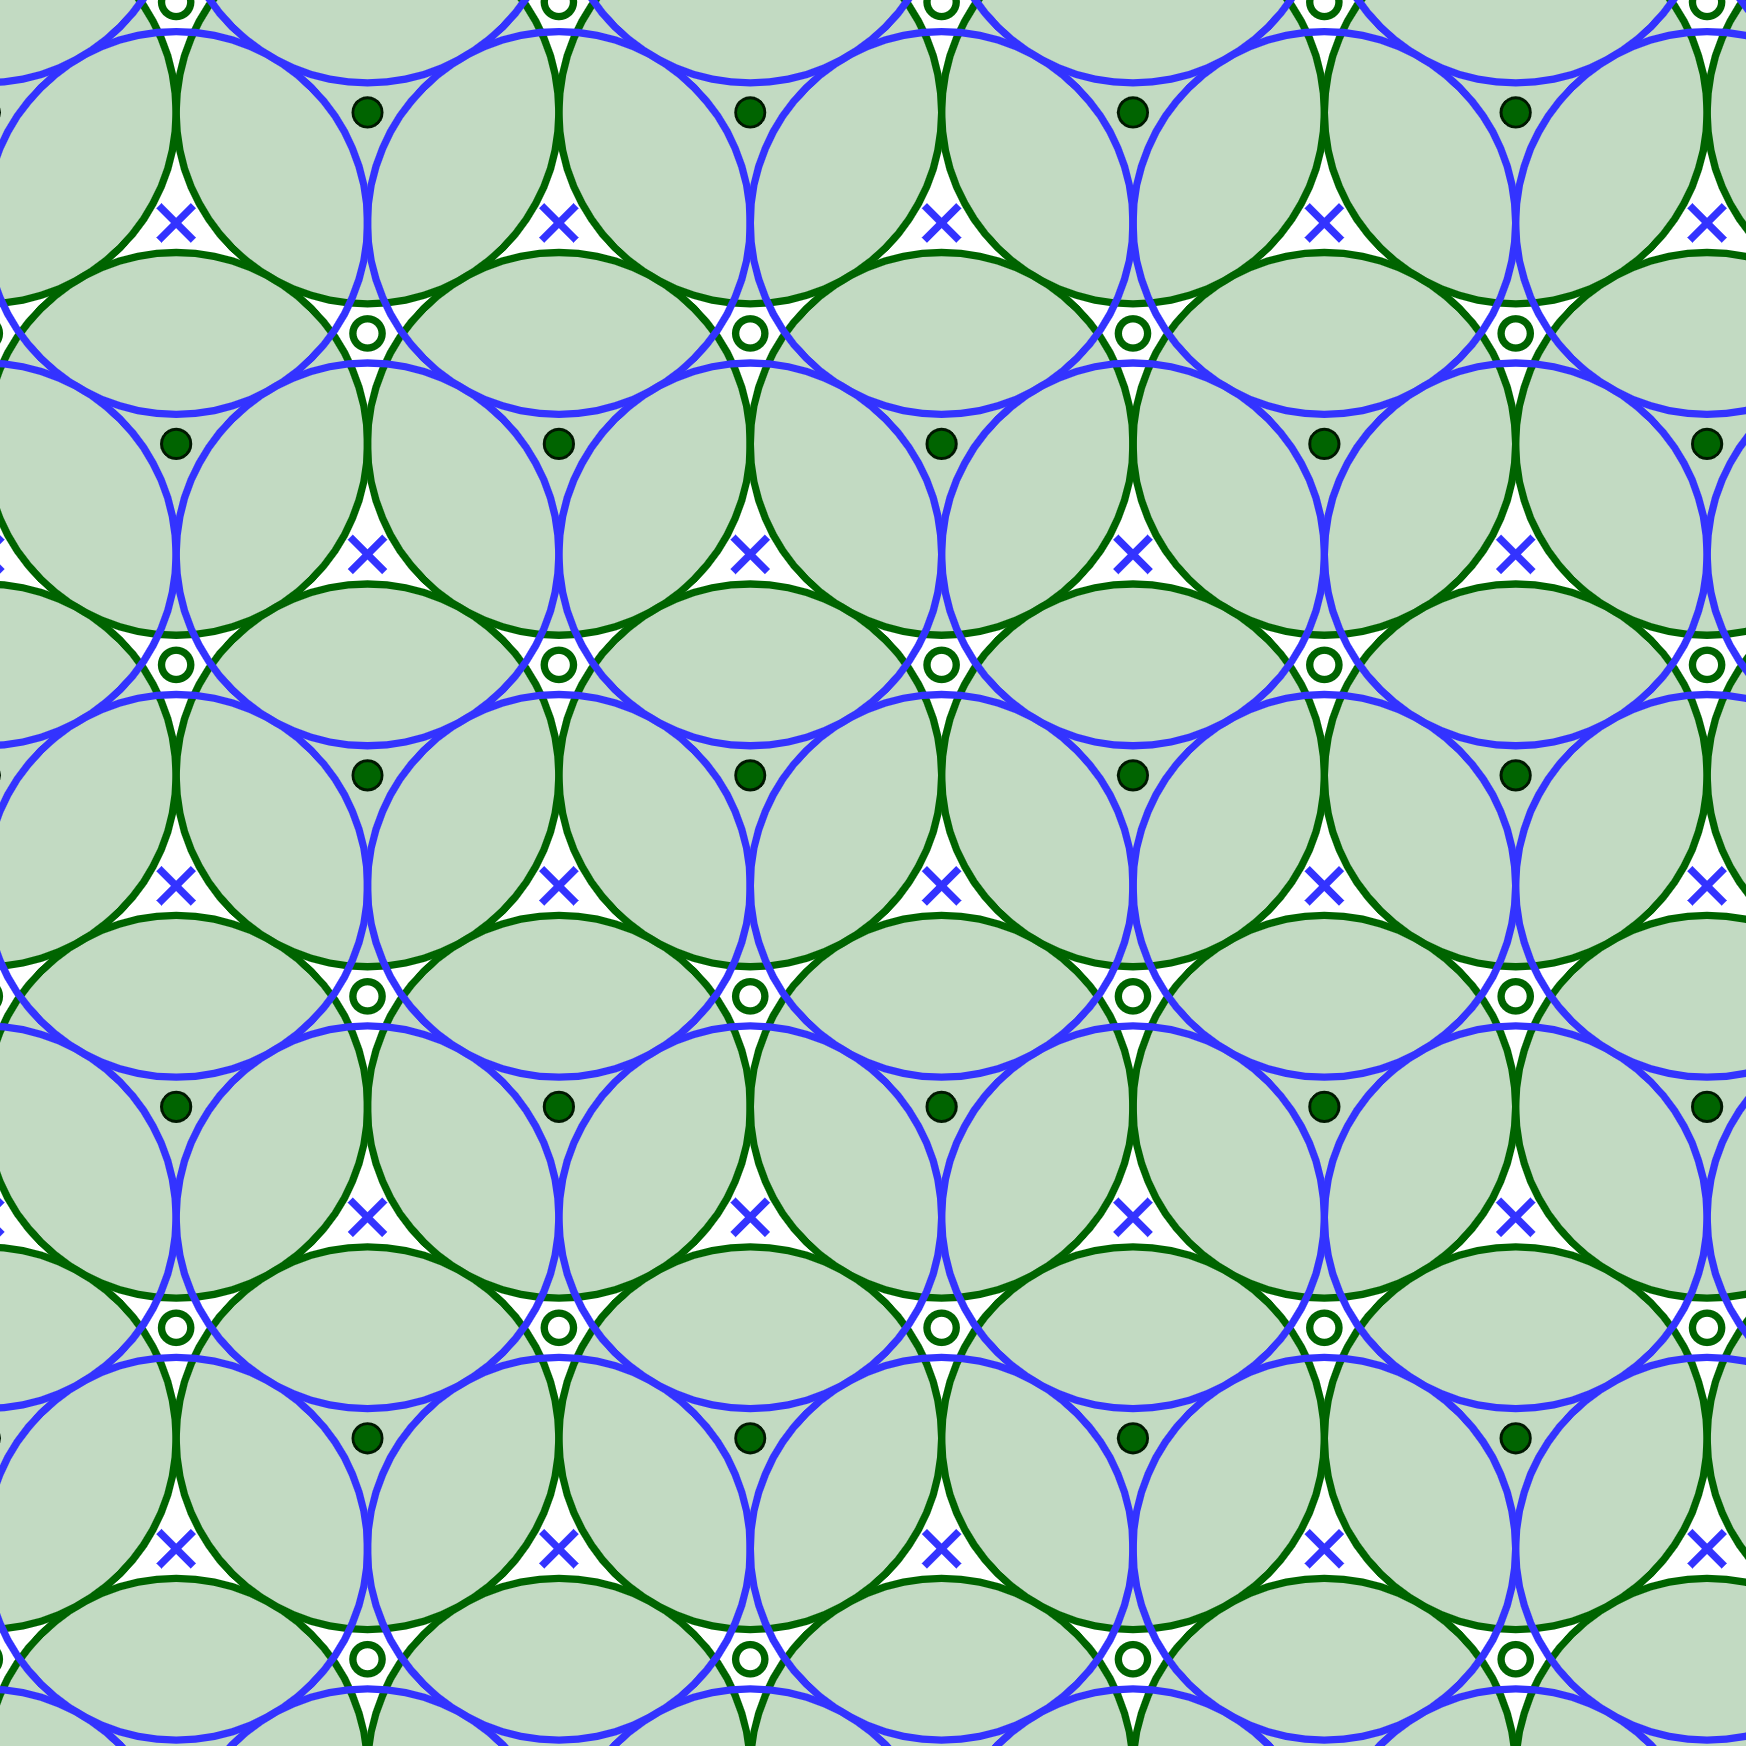
\includegraphics[scale=1]{Ch10/ClosestPacking/ClosestPacking2}
	\caption{Two layers of closest packing}
	\label{closestpack_1}
\end{figure}\ \\
%
If we add a second layer, we can either put spheres on $\Delta$ sites or $\nabla$ sites, 
and create an identical but translated closest pack layer. We call these three layers $A,B$ and $C$.
The correspondence doesn't matter, so does which layer is put on the cell vertices, 
but for convenience and clarity, $A,B,C$ layers will be denoted as $\bullet,\times,\circ$ respectively. 
Within a plane projection from $c$ axis, we can pick a hexagonal unit cell for them, which looks like figure \ref{closestpack_11}.\\
%
\begin{figure}[h]
	\centering
	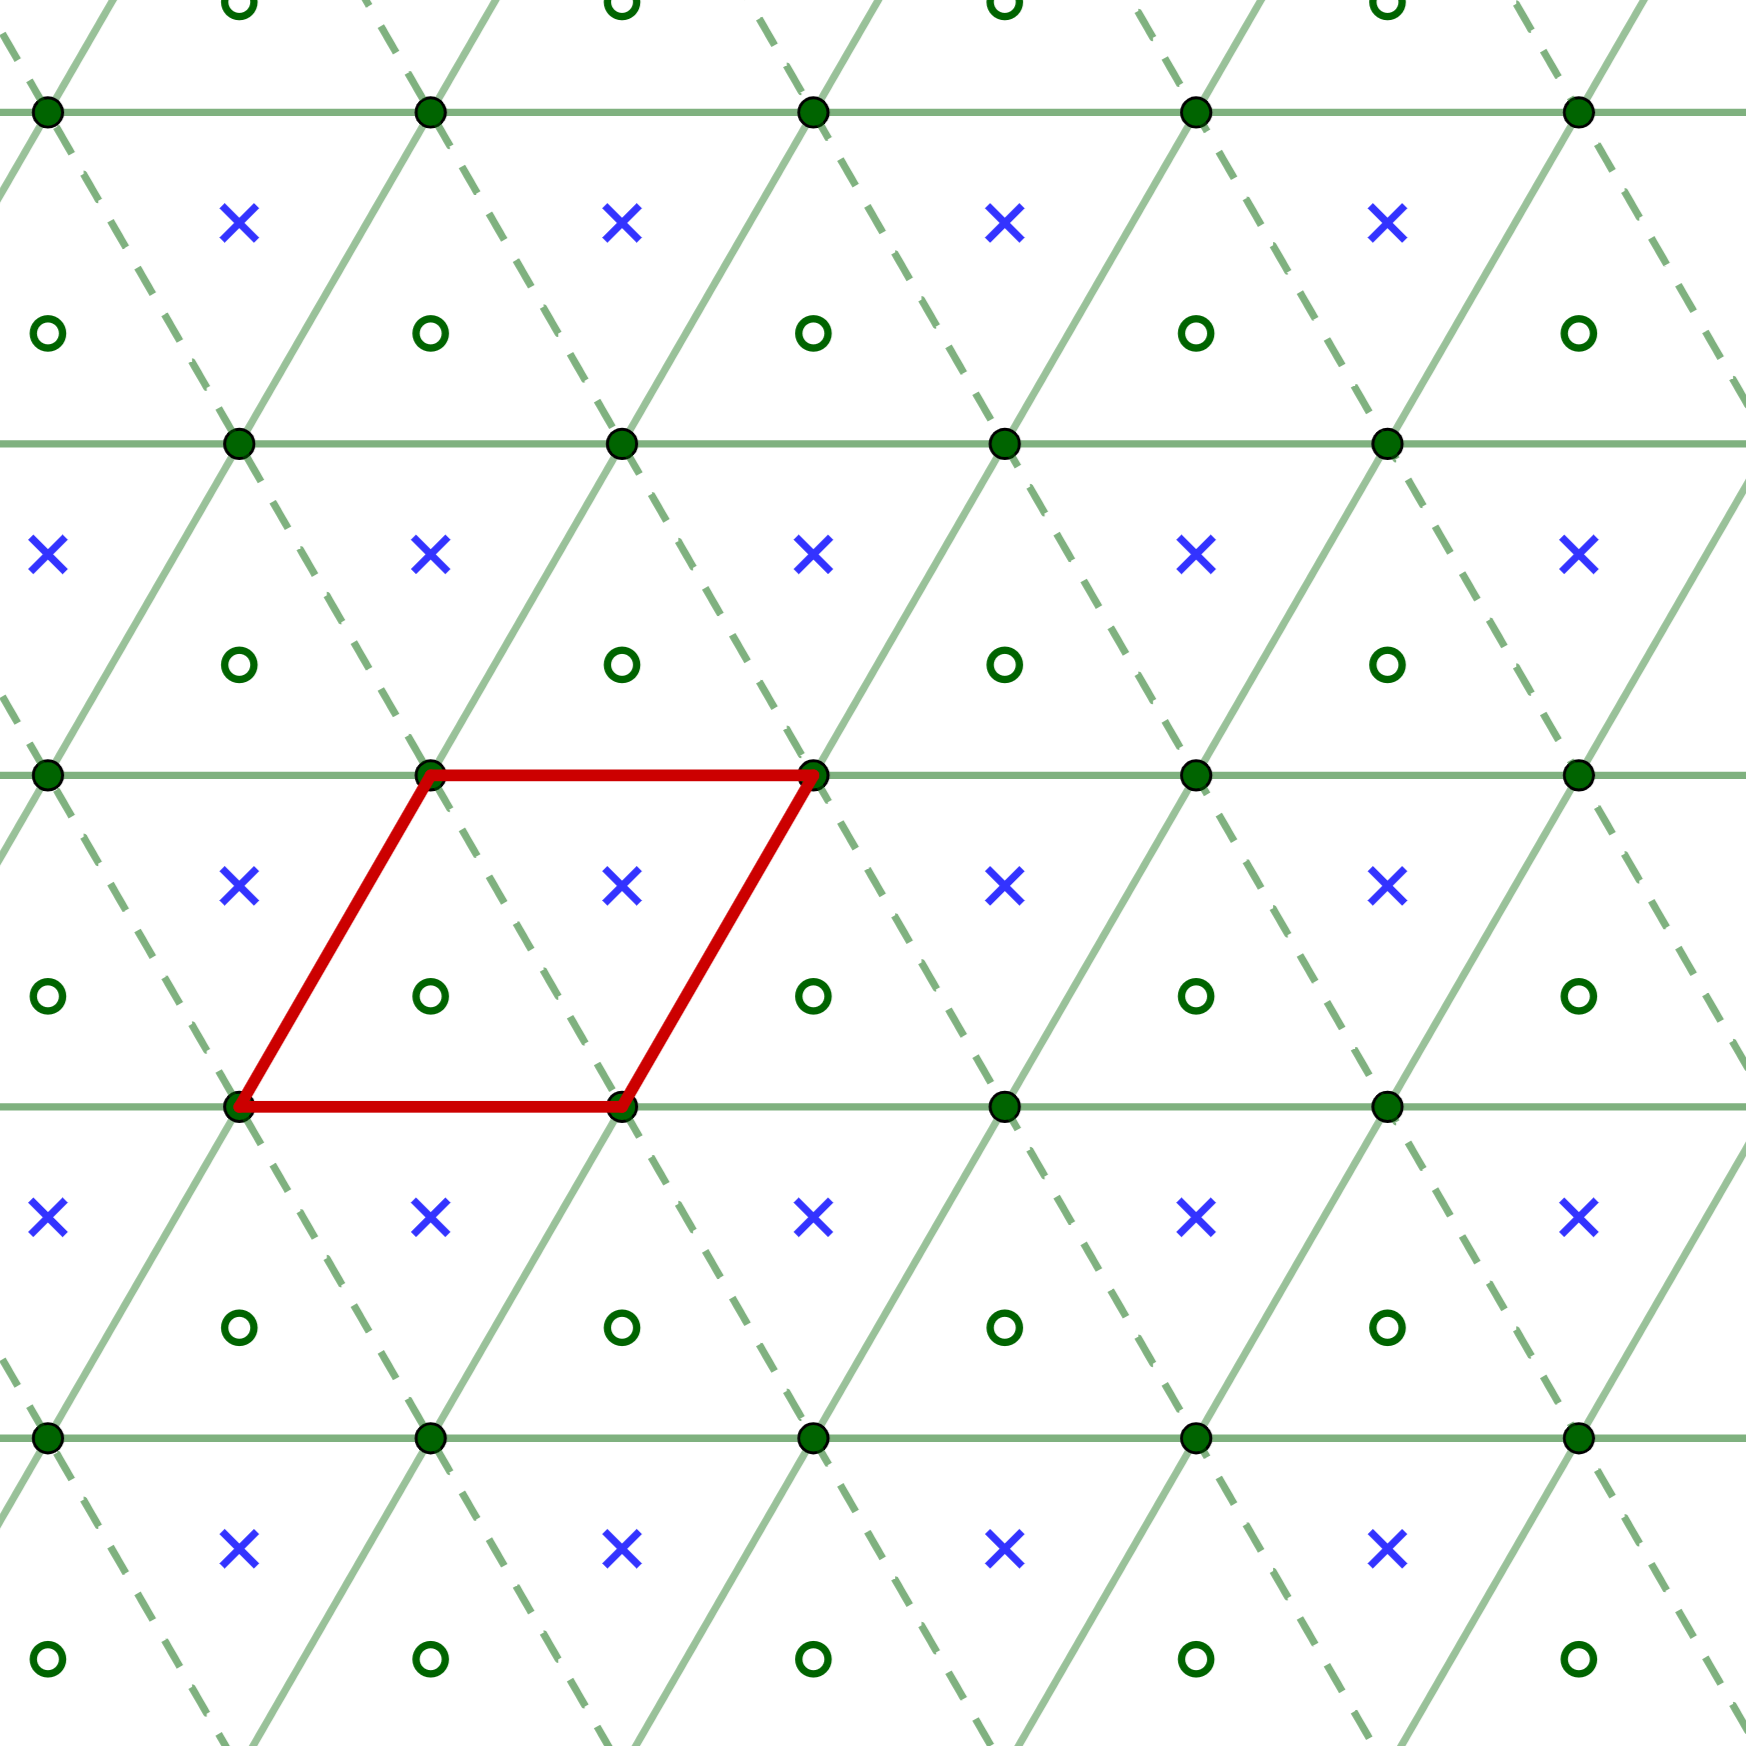
\includegraphics[scale=1]{Ch10/ClosestPacking/ClosestPacking3}
	\quad
	\includegraphics[scale=1]{Ch10/ClosestPacking/voids1}
	\caption{Unit cell projection along $c$}
	\caption{Tetrahedral and octahedral interstices projection along $c$}
	\label{closestpack_11}
\end{figure}\ \\
%
Two layers $AB$ are constructed, and between the two layers there're two types of sites: tetrahedral and octahedral. 
An octahedral site lands right on the position for $C$, and a tetrahedral site based on $A$ coincide with $B$, vice versa.
And as the center of octahedral site lies right in the middle while tetrahedral centers are located $1/4$ layer distance above its base. 
\label{tetrahedralsite}
If we use lowercase $a,b,c$ to denote site centers, then between two layers the model can be expressed as:
%
\[
	|\ A\ b^{T}\ c^{O}\ a^{T} B \ a^{T}\ c^{O}\ b^{T}|\ A\cdots
\]
%
where a pair of $||$ denotes a minimal repitition unit for this $ABABAB\cdots$ packing paradigm. 
Consequently, the number of octahedral sites are equal to that of spheres which are half of tetrahedral sites.\\ 
And after a little bit of math, we obtain that the height of tetrahedra and octahedra with the same edge length are the same 
as they both corresponds to the layer distance:
%
\[
	h_{O}=h_{T}=\frac{\sqrt{6}}{3}a
\]
%
\begin{figure}[h]
	\centering
	\includegraphics[scale=0.02]{Ch10/ClosestPacking/octahedron}
	\includegraphics[scale=0.025]{Ch10/ClosestPacking/tetrahedron}
	\caption{3 dimentional figure of octahedral and tetrahedral sites}
\end{figure}
%
But when adding the third layer, there are two ways, namely hexagonal and cubic.
%
\subsection{Hexagonal Closest-Packing}
%
If we keep adding only two kinds of layers and forming structure like $ABABAB\cdots$, 
this form of packing have a $6_3$ screw axis 
(and a gilde plane, obvious in figure \ref{hcp1}, though it's not as `standard'), 
so it's called hexagonal closest packing.
%
\begin{figure}[h]
	\centering
	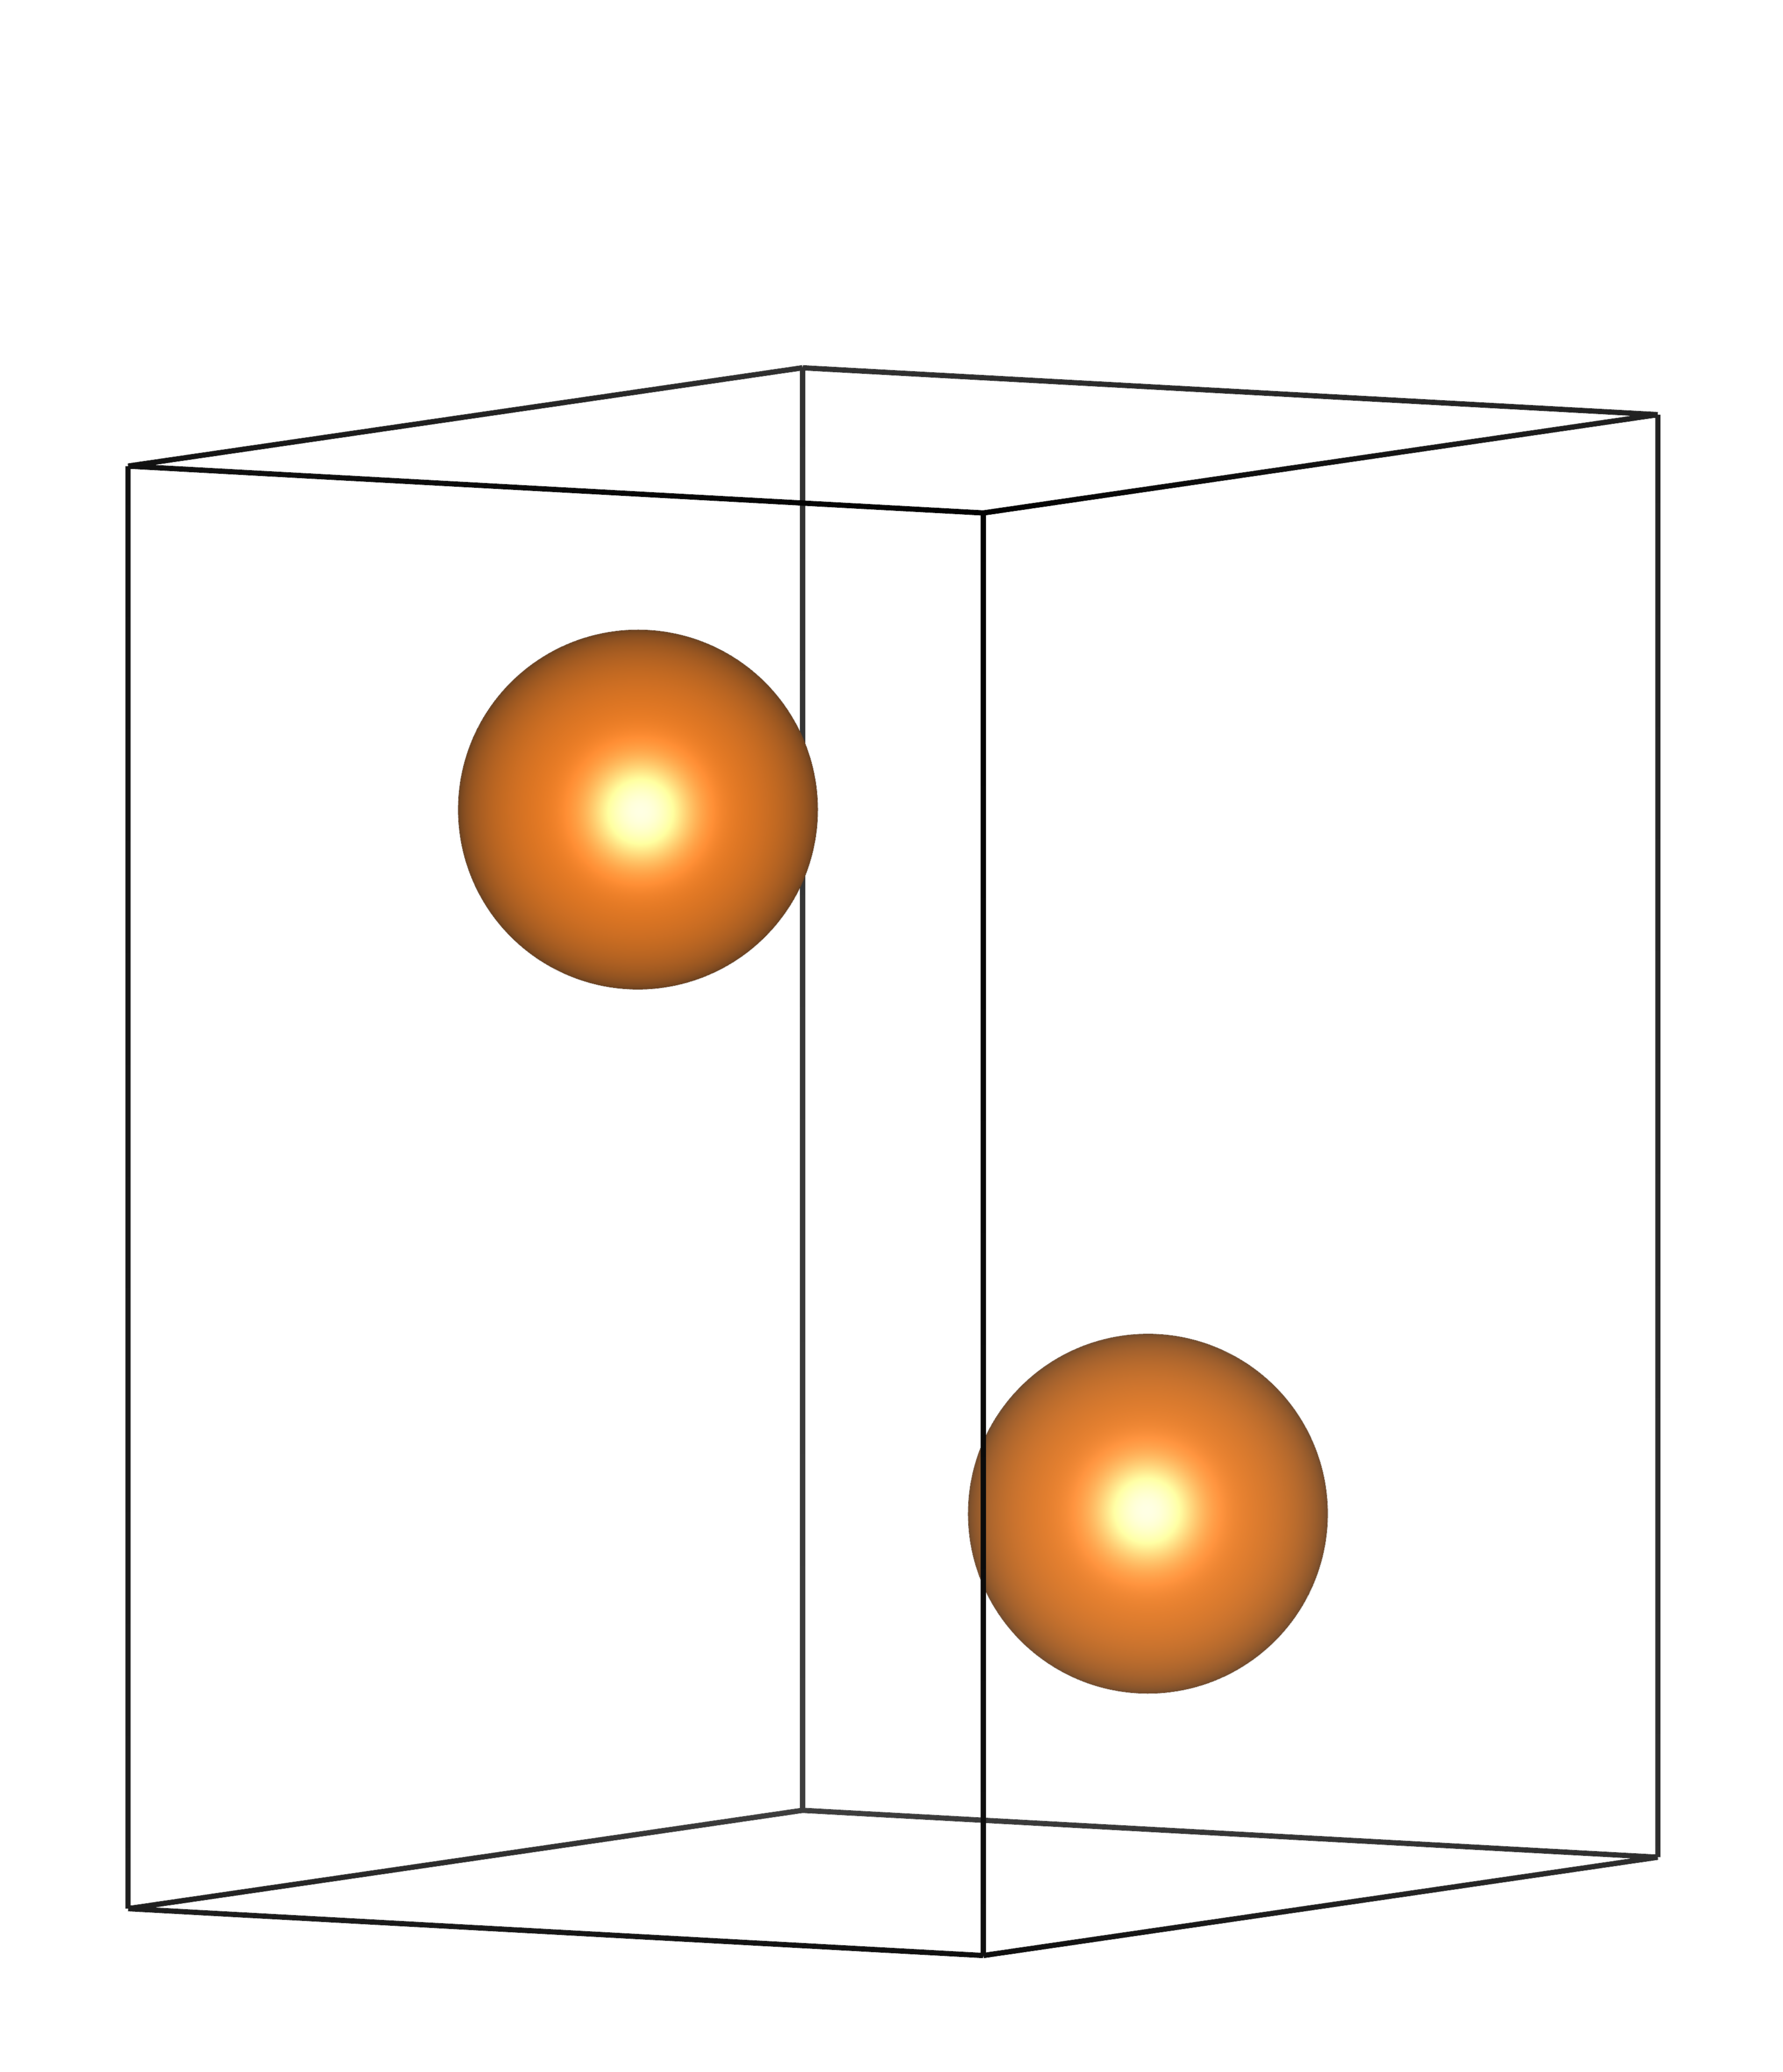
\includegraphics[scale=0.04]{Ch10/ClosestPacking/hcp}
	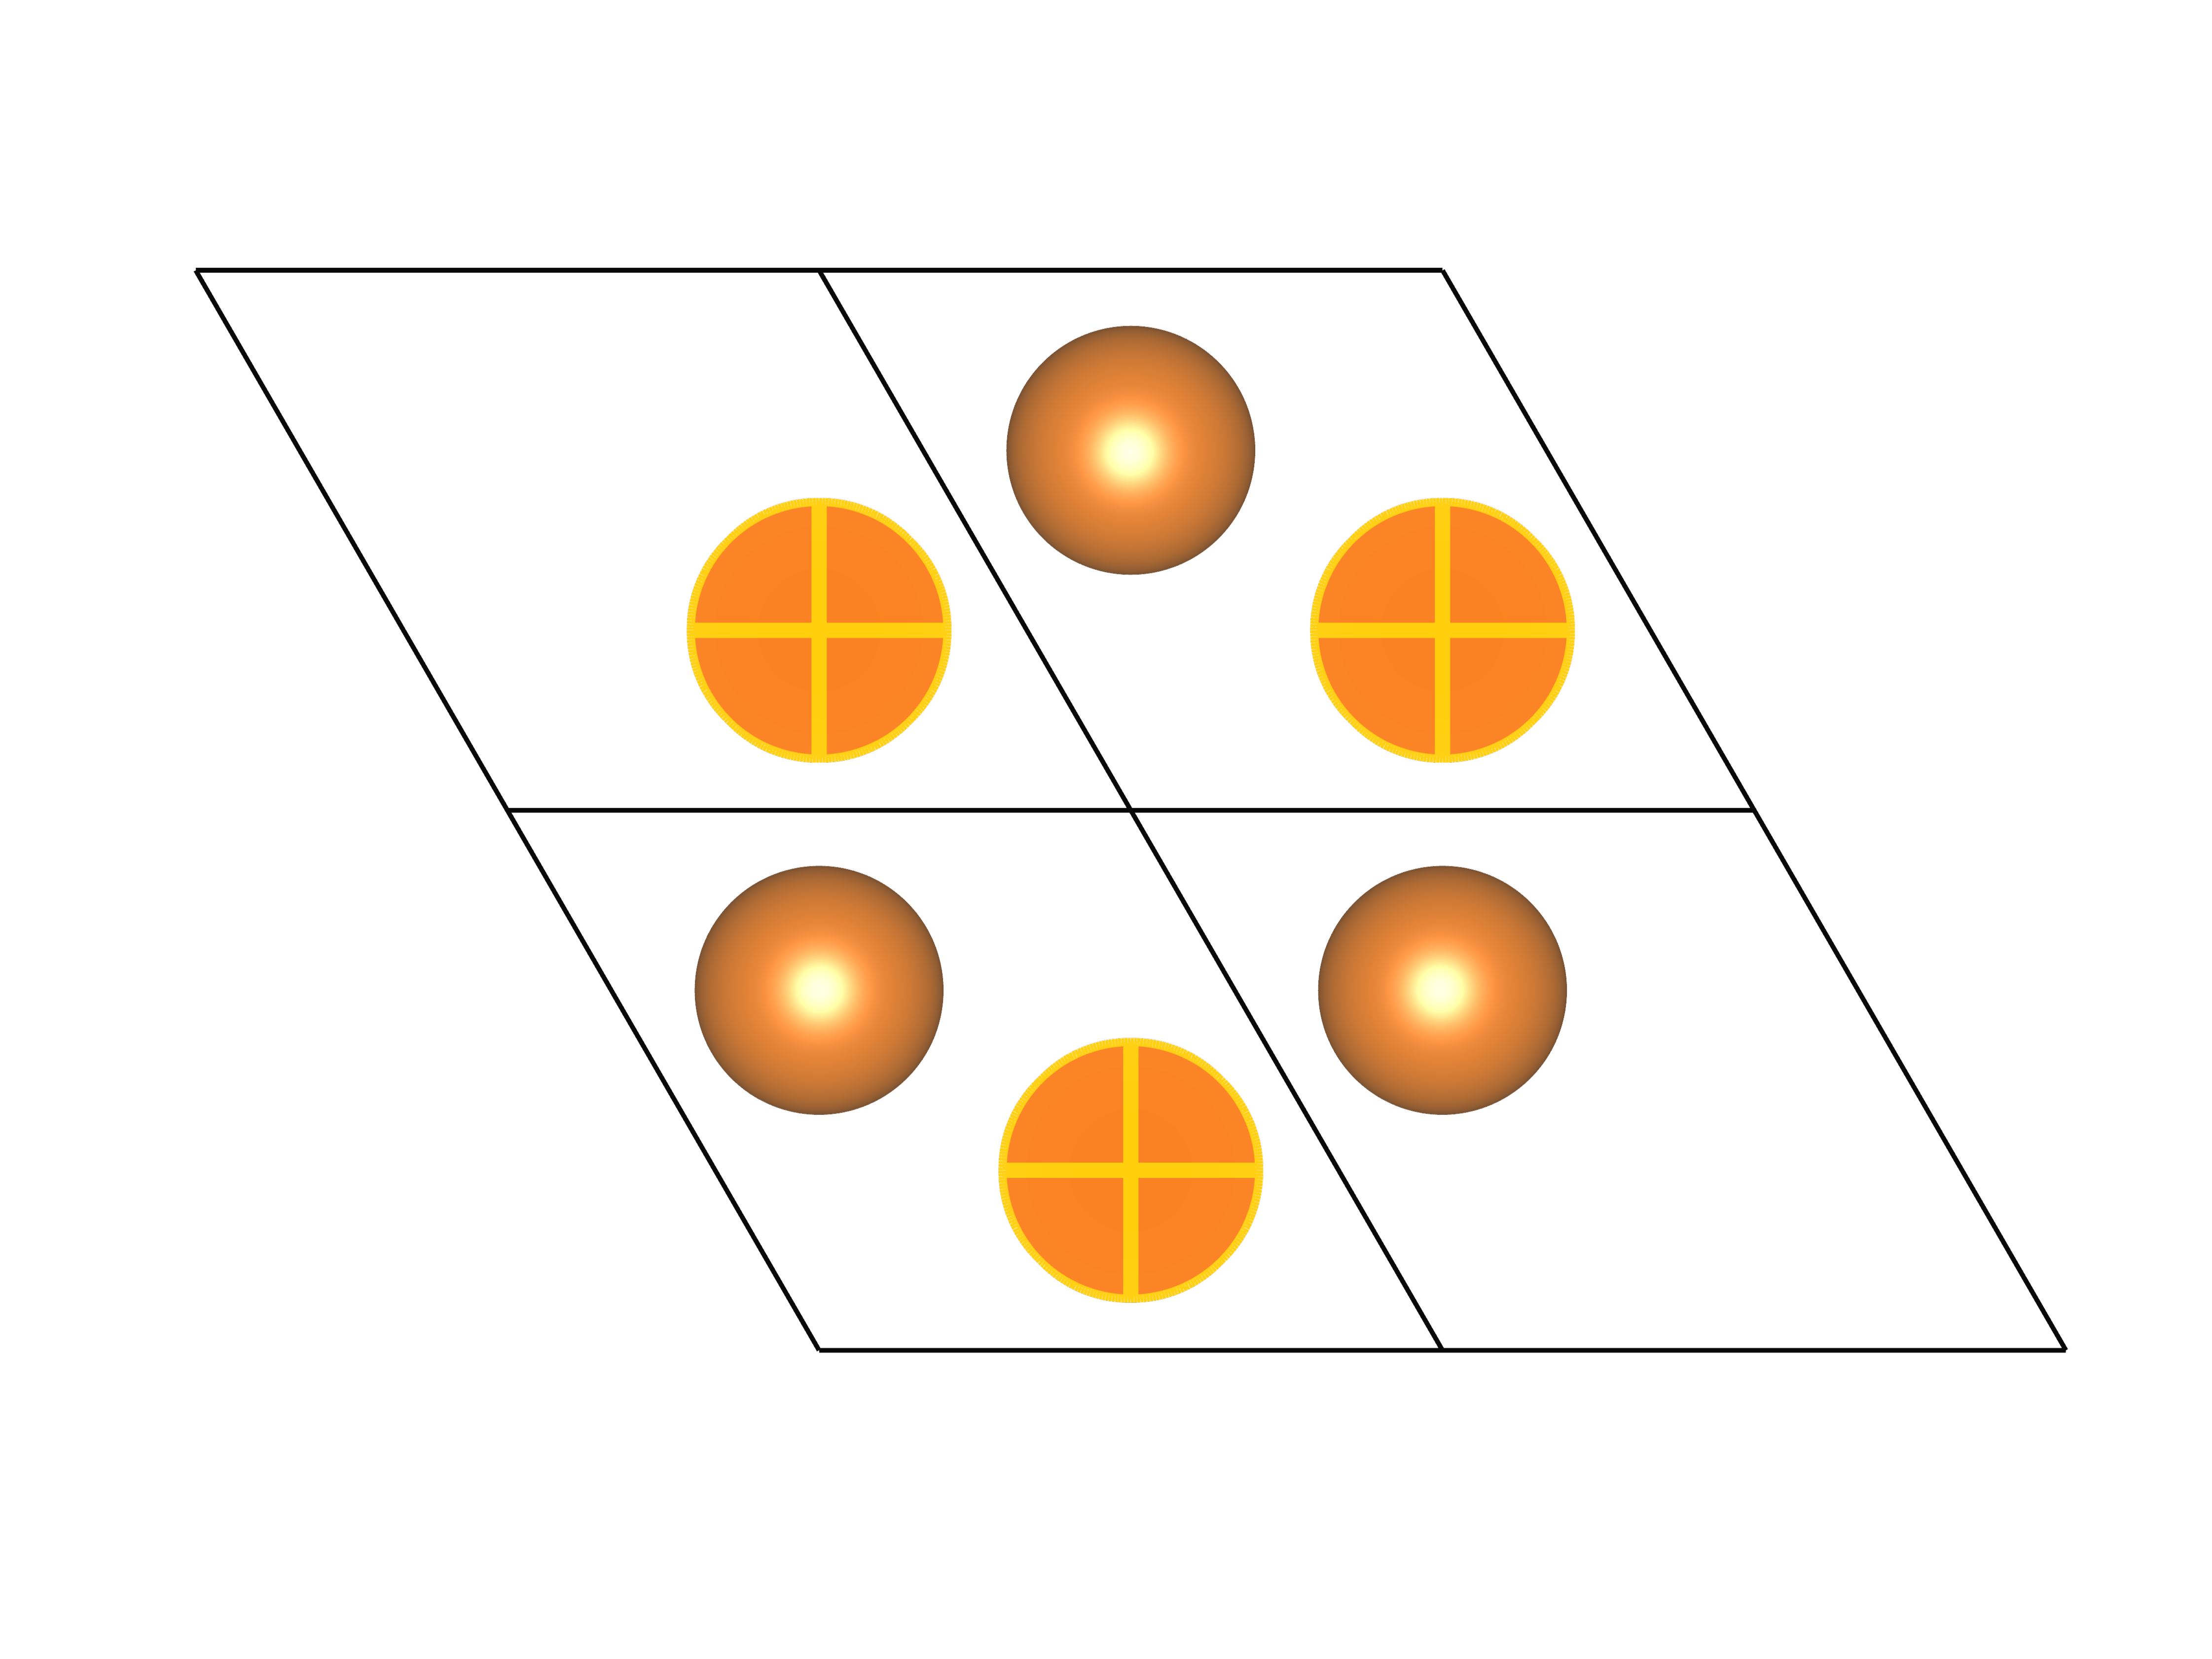
\includegraphics[scale=0.04]{Ch10/ClosestPacking/hcp63}
	\caption{Hexagonal closest packing, $hP$, structural motif 2 chemical formula}
	\label{hcp1}
\end{figure}
%
In figure \ref{hcp1} we put the octahedral sites $c$ on the vertices. 
If the atoms are placed at the vertices, the places of octahedral and tetrahedral sites are listed in table \ref{hcpsite}.
%
\begin{figure}[h]
	\centering
	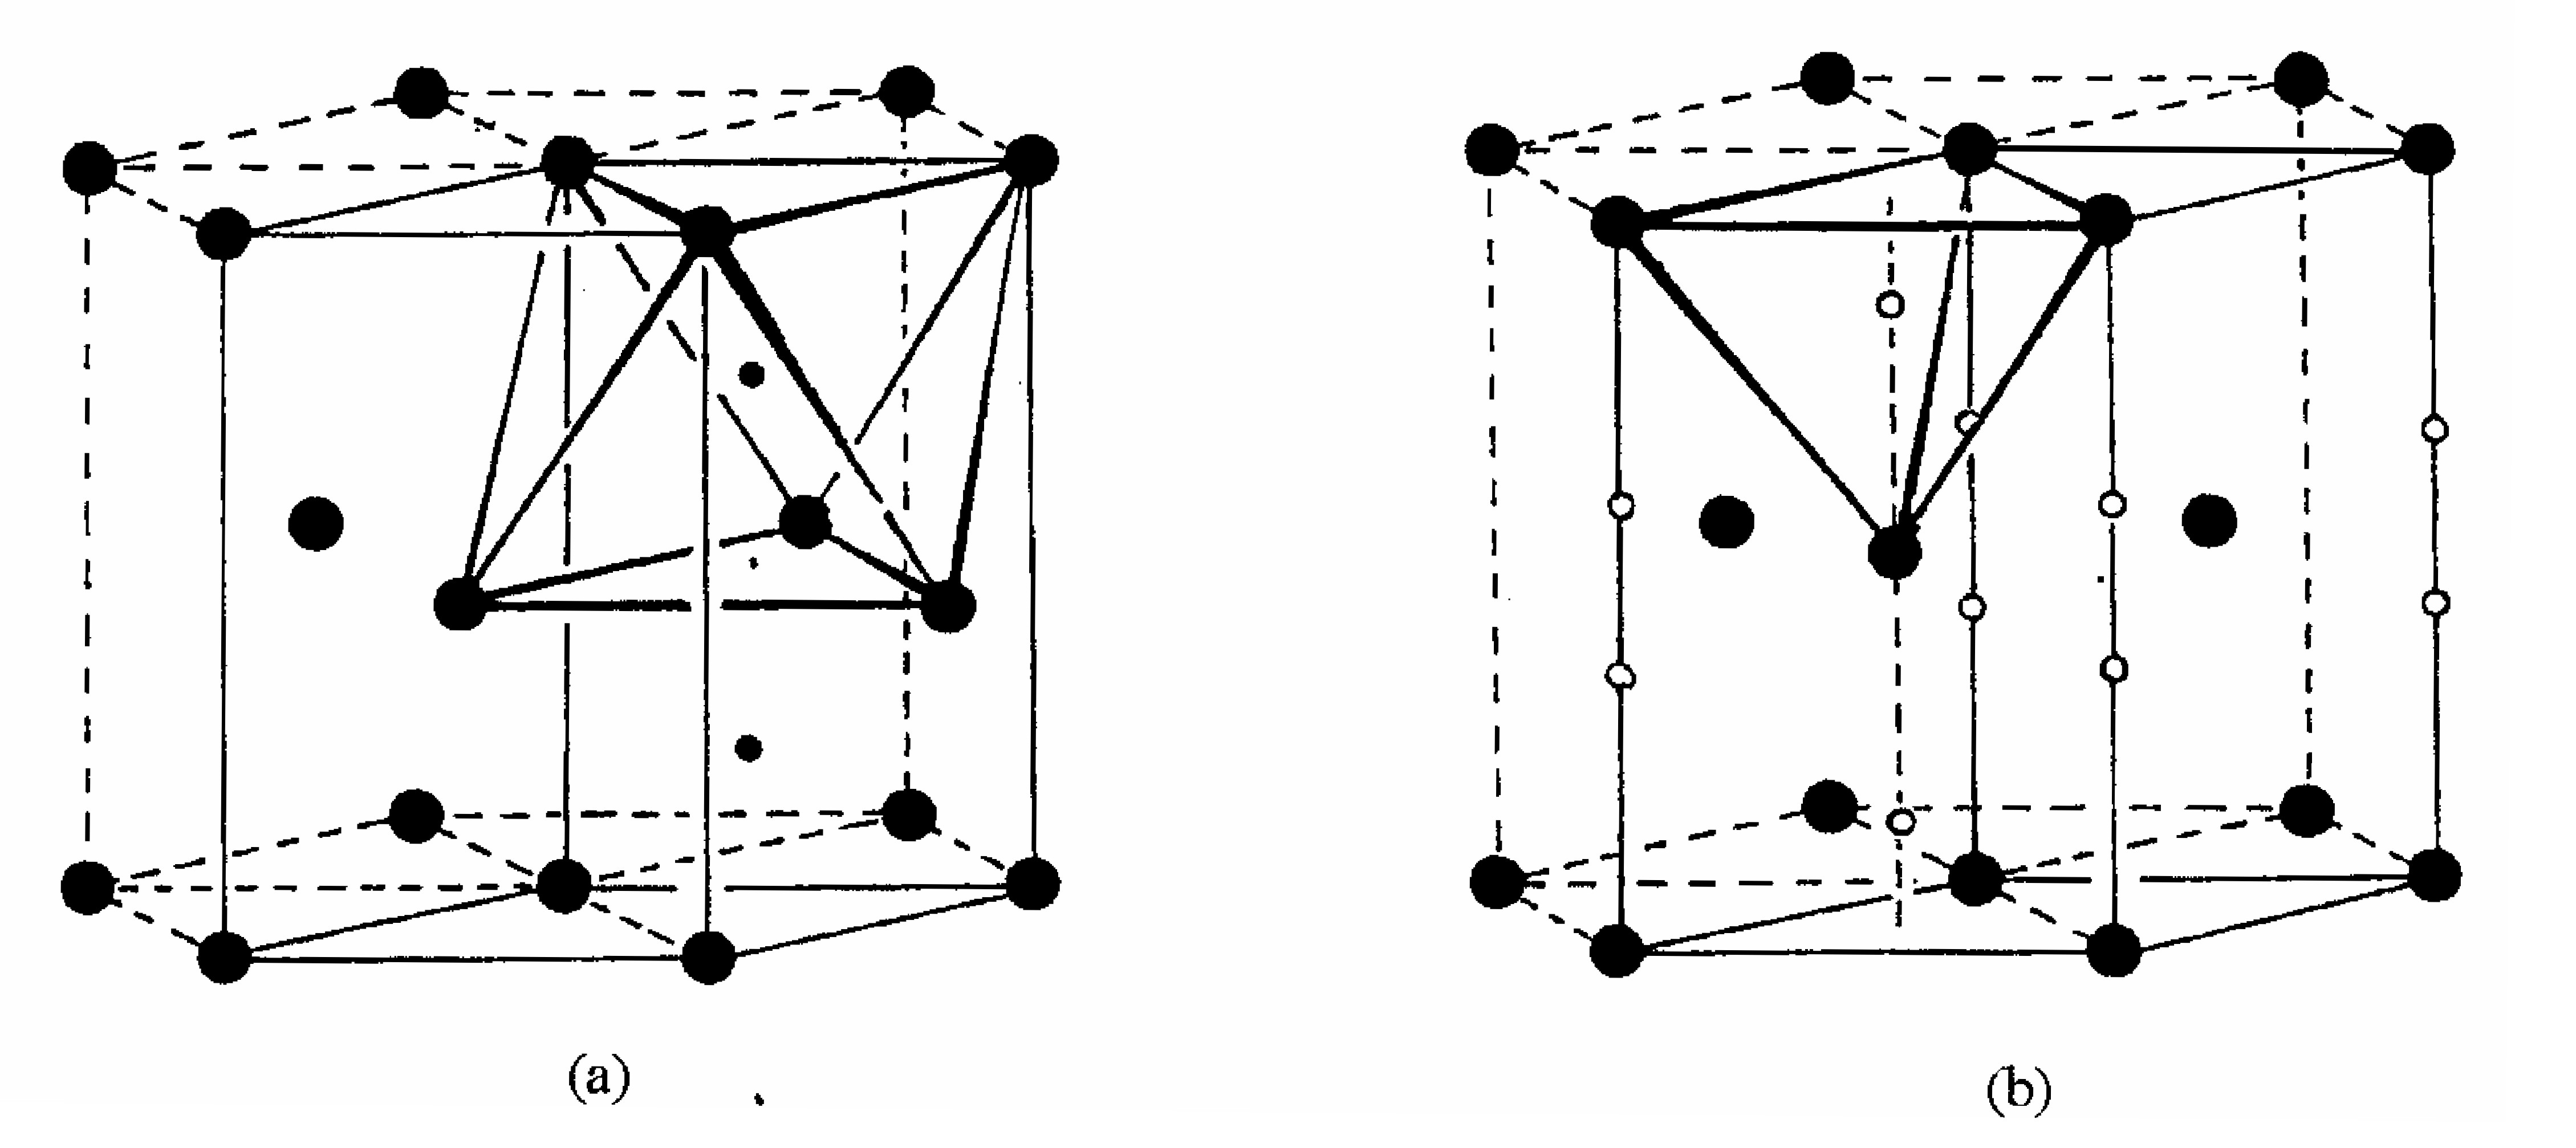
\includegraphics[scale=0.08]{Ch10/ClosestPacking/hcpvoid}
	\caption{Locations of interstices in hcp cells}
\end{figure}
%
\begin{table}
	\centering
	\begin{tabular}{@{}ll@{}}
		\toprule
		\ \textbf{Items}	& \textbf{Coordinates}											\\
		\midrule
		\ Atoms				& (0, 0, 0), (1/3, 1/3, 1/2)									\\
		\ Octahedral Sites	& (1/3, 2/3, 1/4), (1/3, 2/3, 3/4)								\\
		\ Tetrahedral Sites	& (0, 0, 3/8), (0, 0, 5/8), (1/3, 1/3, 1/8), (1/3, 1/3, 7/8)\	\\
		\bottomrule
	\end{tabular}
	\caption{interstice sites in hcp}
	\label{hcpsite}
\end{table}
%
Playing around with the symmetry operations and one will find that: if layer $A$ is at the vertices, 
%
\begin{itemize}
	\item 3 along the edge preserves all closest pack layers;
	\item 6 along the edge exchanges $B$ and $C$ without affecting $A$;
	\item $\bar{1}$ at the center exchanges $B$ and $C$ without affecting $A$ and maps coordinate $c$ to $1-c$.
\end{itemize}
%
Therefore other forms of packing can also have six-fold symmetry. Examples applying 6:
%
\[
	|\ ABCACB\ |\ ABCACB\cdots\ \to\ |\ ACBABC\ |\ ACBABC\cdots\ \ 
	\text{possesses }6_3\text{ and }\bar{6}
\]
%
Often, a $\bar{6}$ axis implies a palindromic sequence of layers, as in the example $ABCACBA$.
%
\subsection{Cubic Closest-Packing}
%
The other packing paradigm is invoking all three kinds of layers in the order of $ABCABC\cdots$. 
This type of stacking doesn't have six-fold symmetry but possesses a 3, $\bar{1}$ 
and consequently $\bar{3}$ along the stacking direction.
Amazingly this way of packing have four (or eight if opposite counts) stacking direction 
so it can be arranged into a cubic cell as in figure \ref{ccp1}
%
\begin{figure}[h]
	\centering
	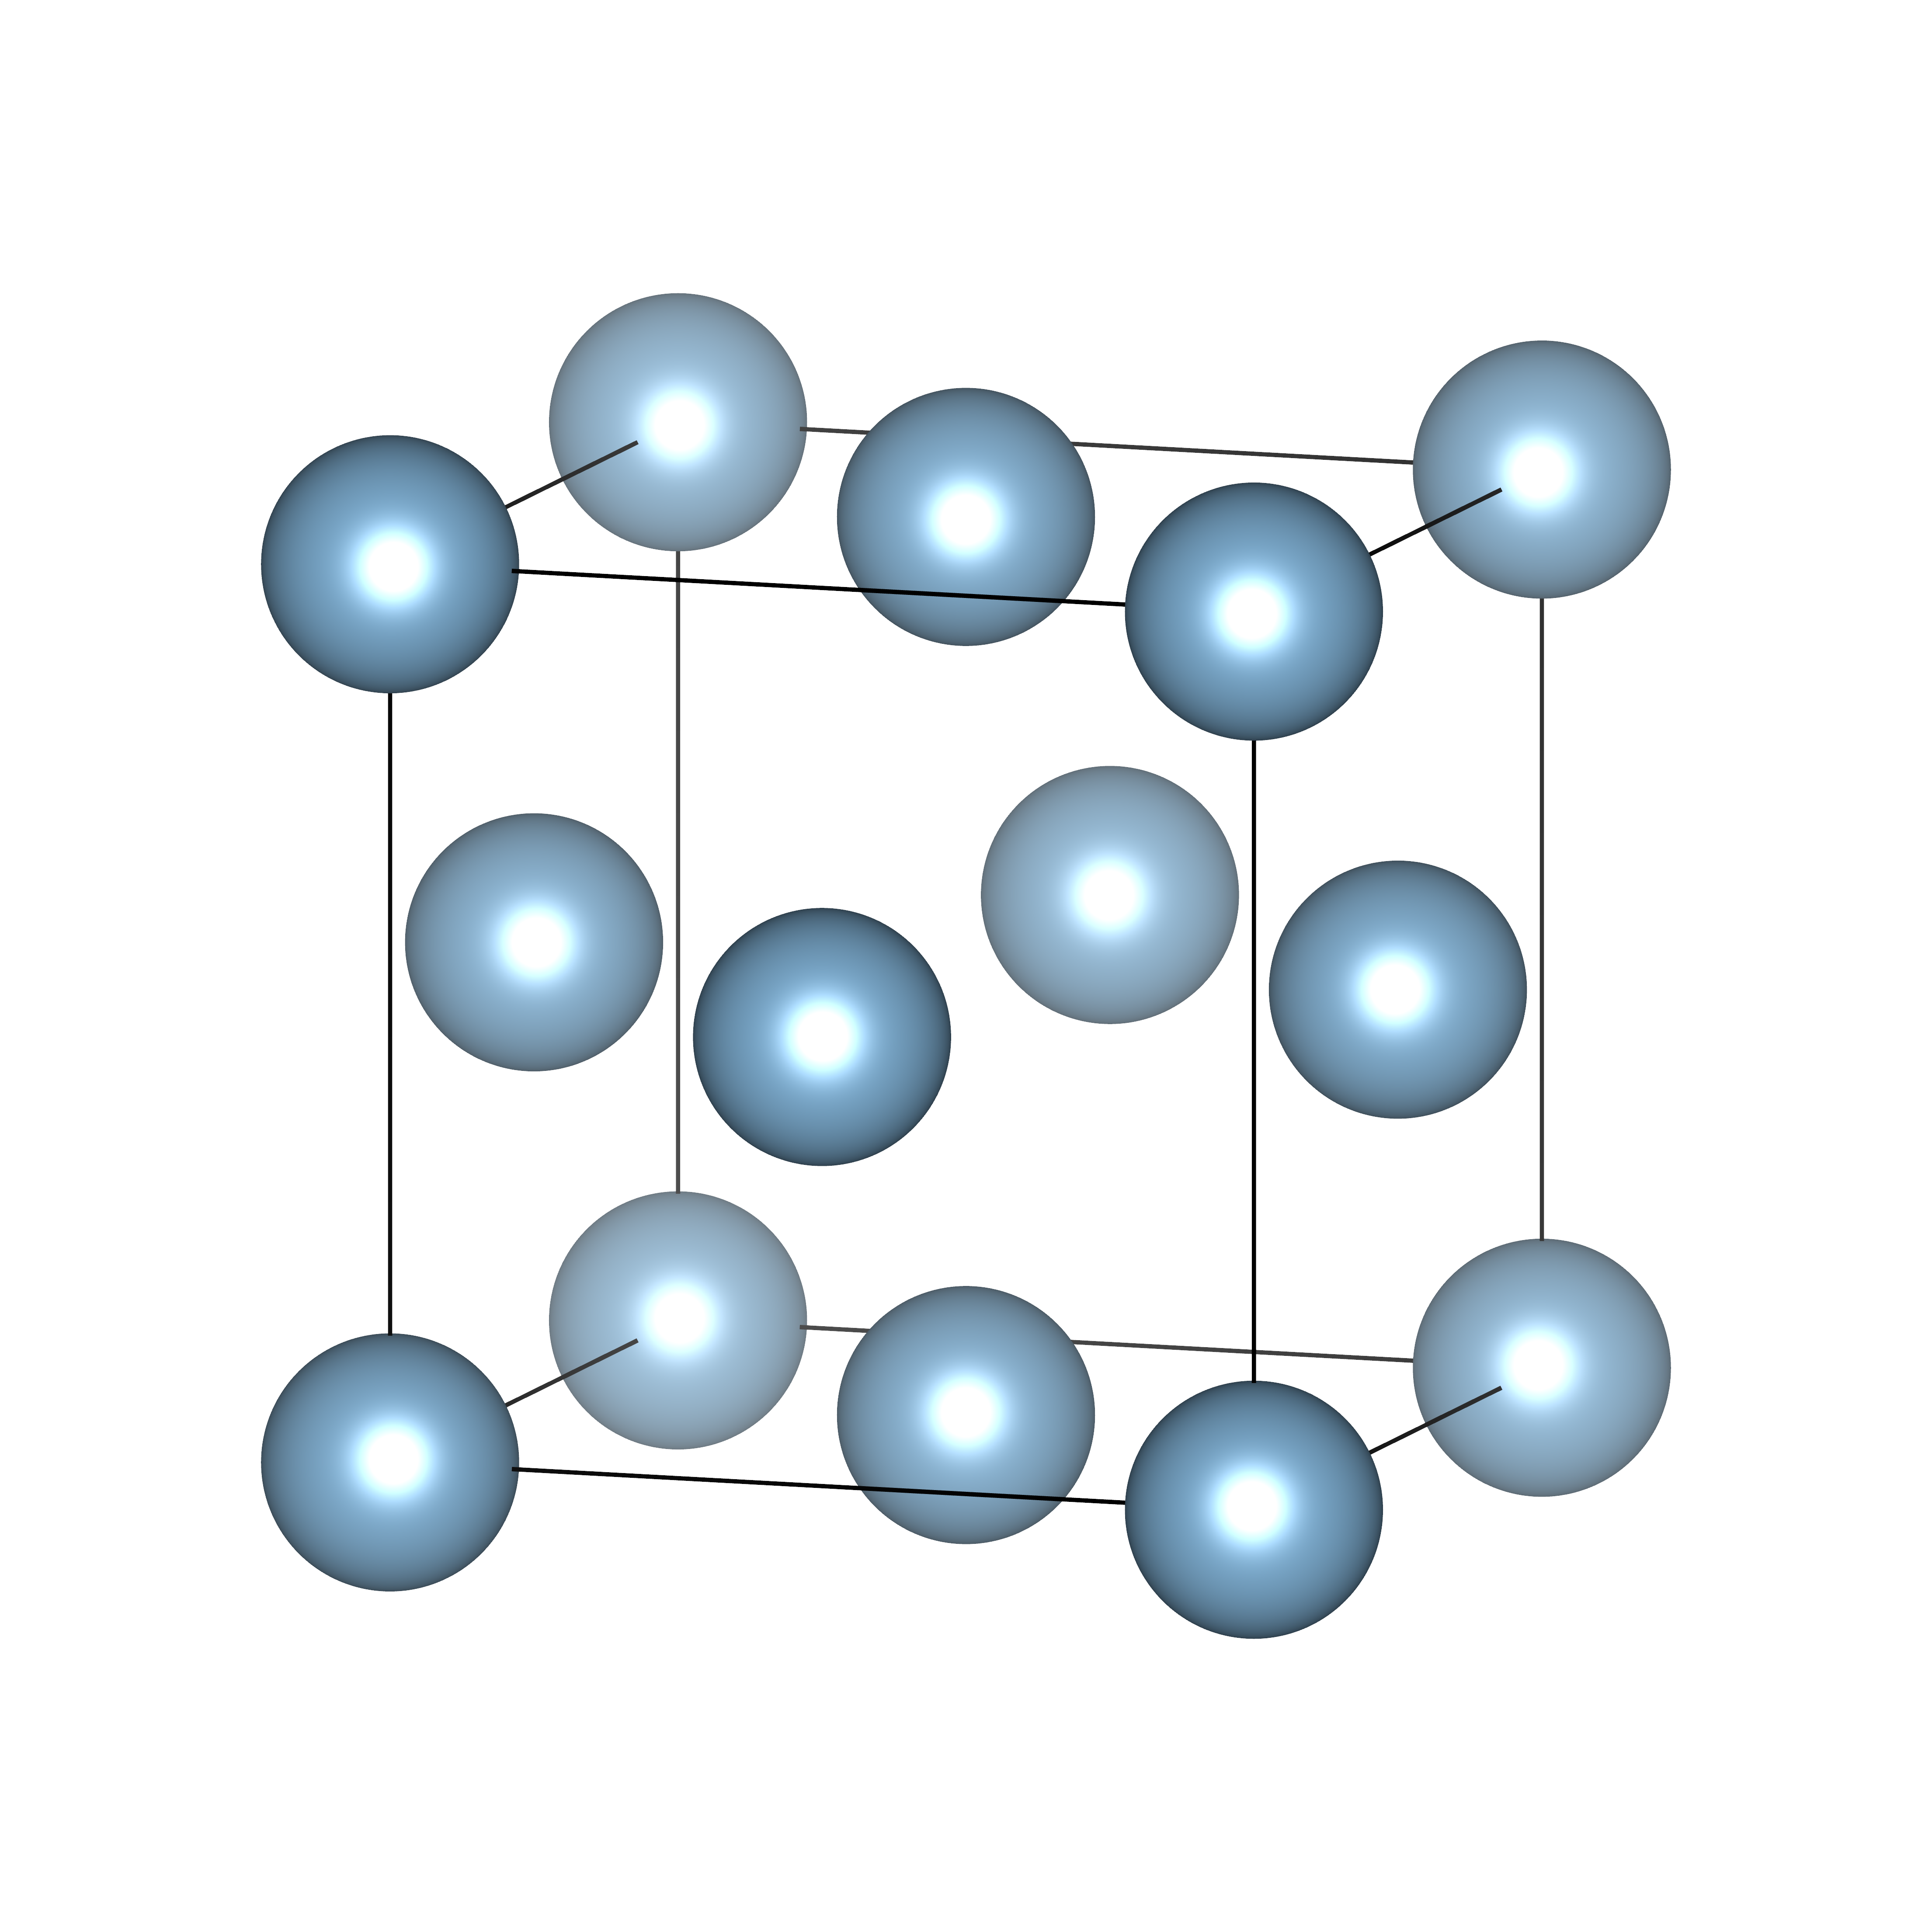
\includegraphics[scale=0.04]{Ch10/ClosestPacking/ccp}
	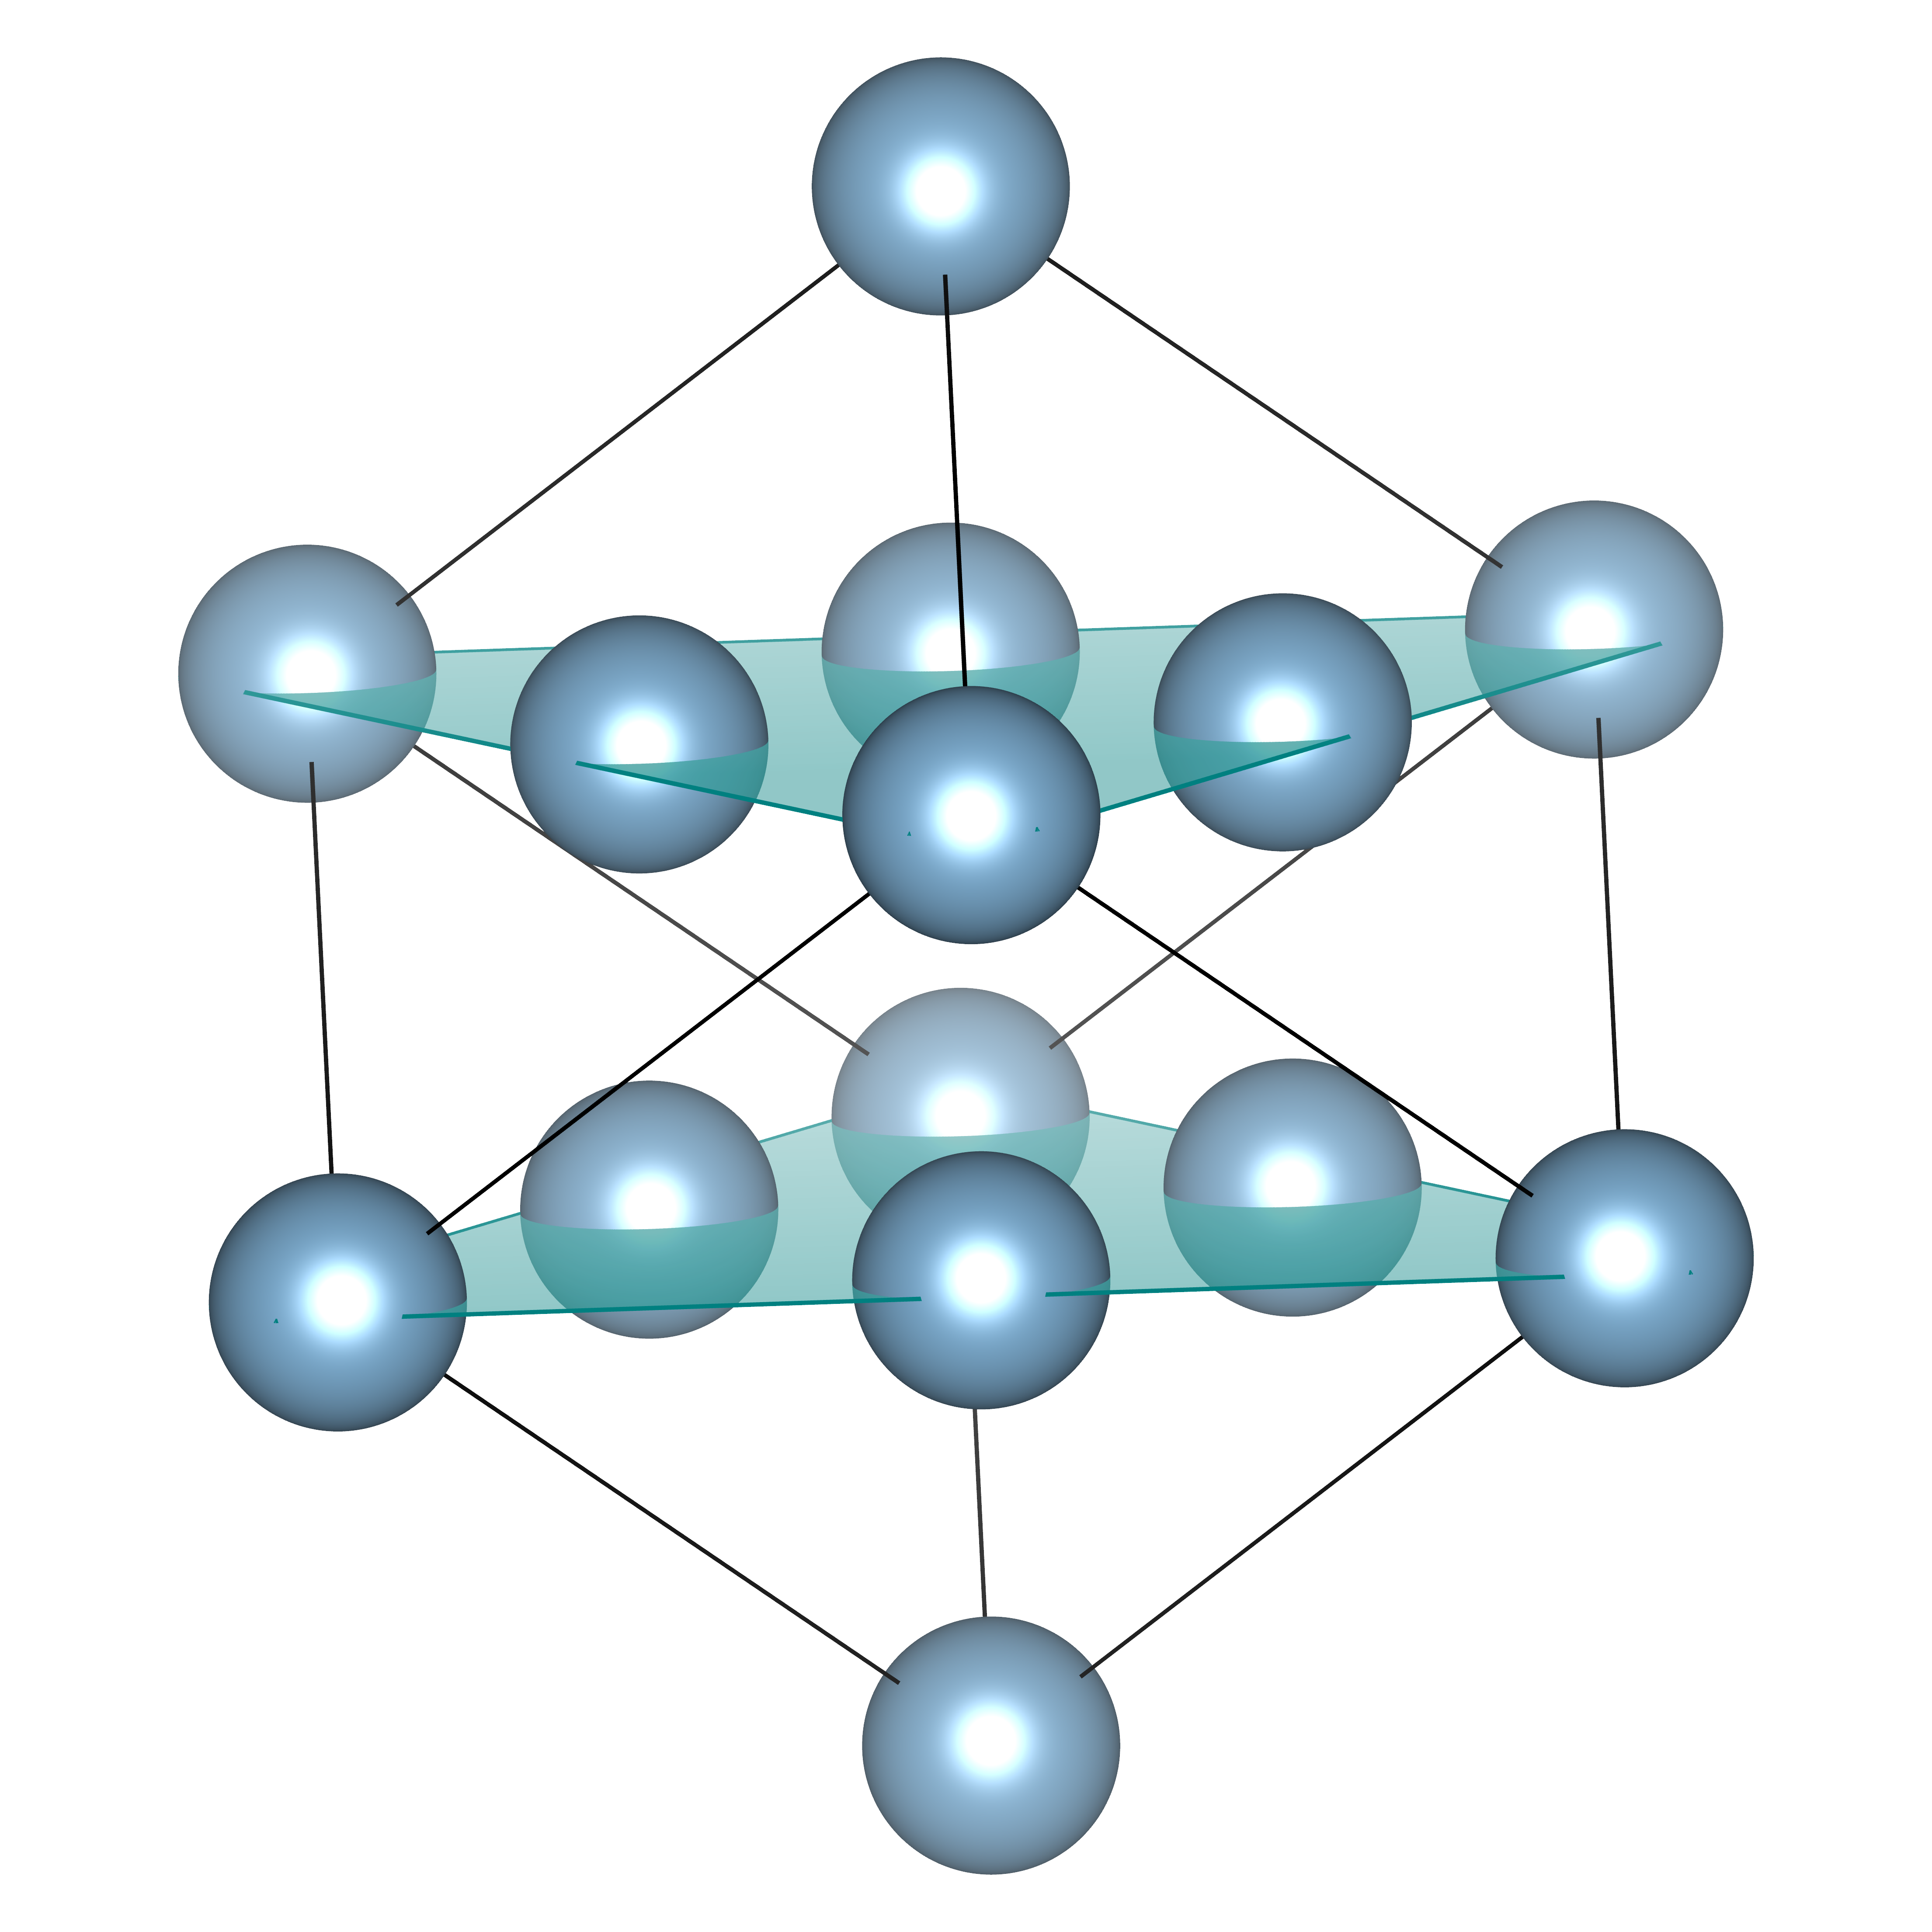
\includegraphics[scale=0.04]{Ch10/ClosestPacking/ccp2}
	\caption{Cubic closest packing, $cF$, structural motif 1 chemical formula}
	\label{ccp1}
\end{figure}\\
%
Its tetrahedral and octahedral sites are listed in table \ref{ccpsite}.
%
\begin{figure}[h]
	\centering
	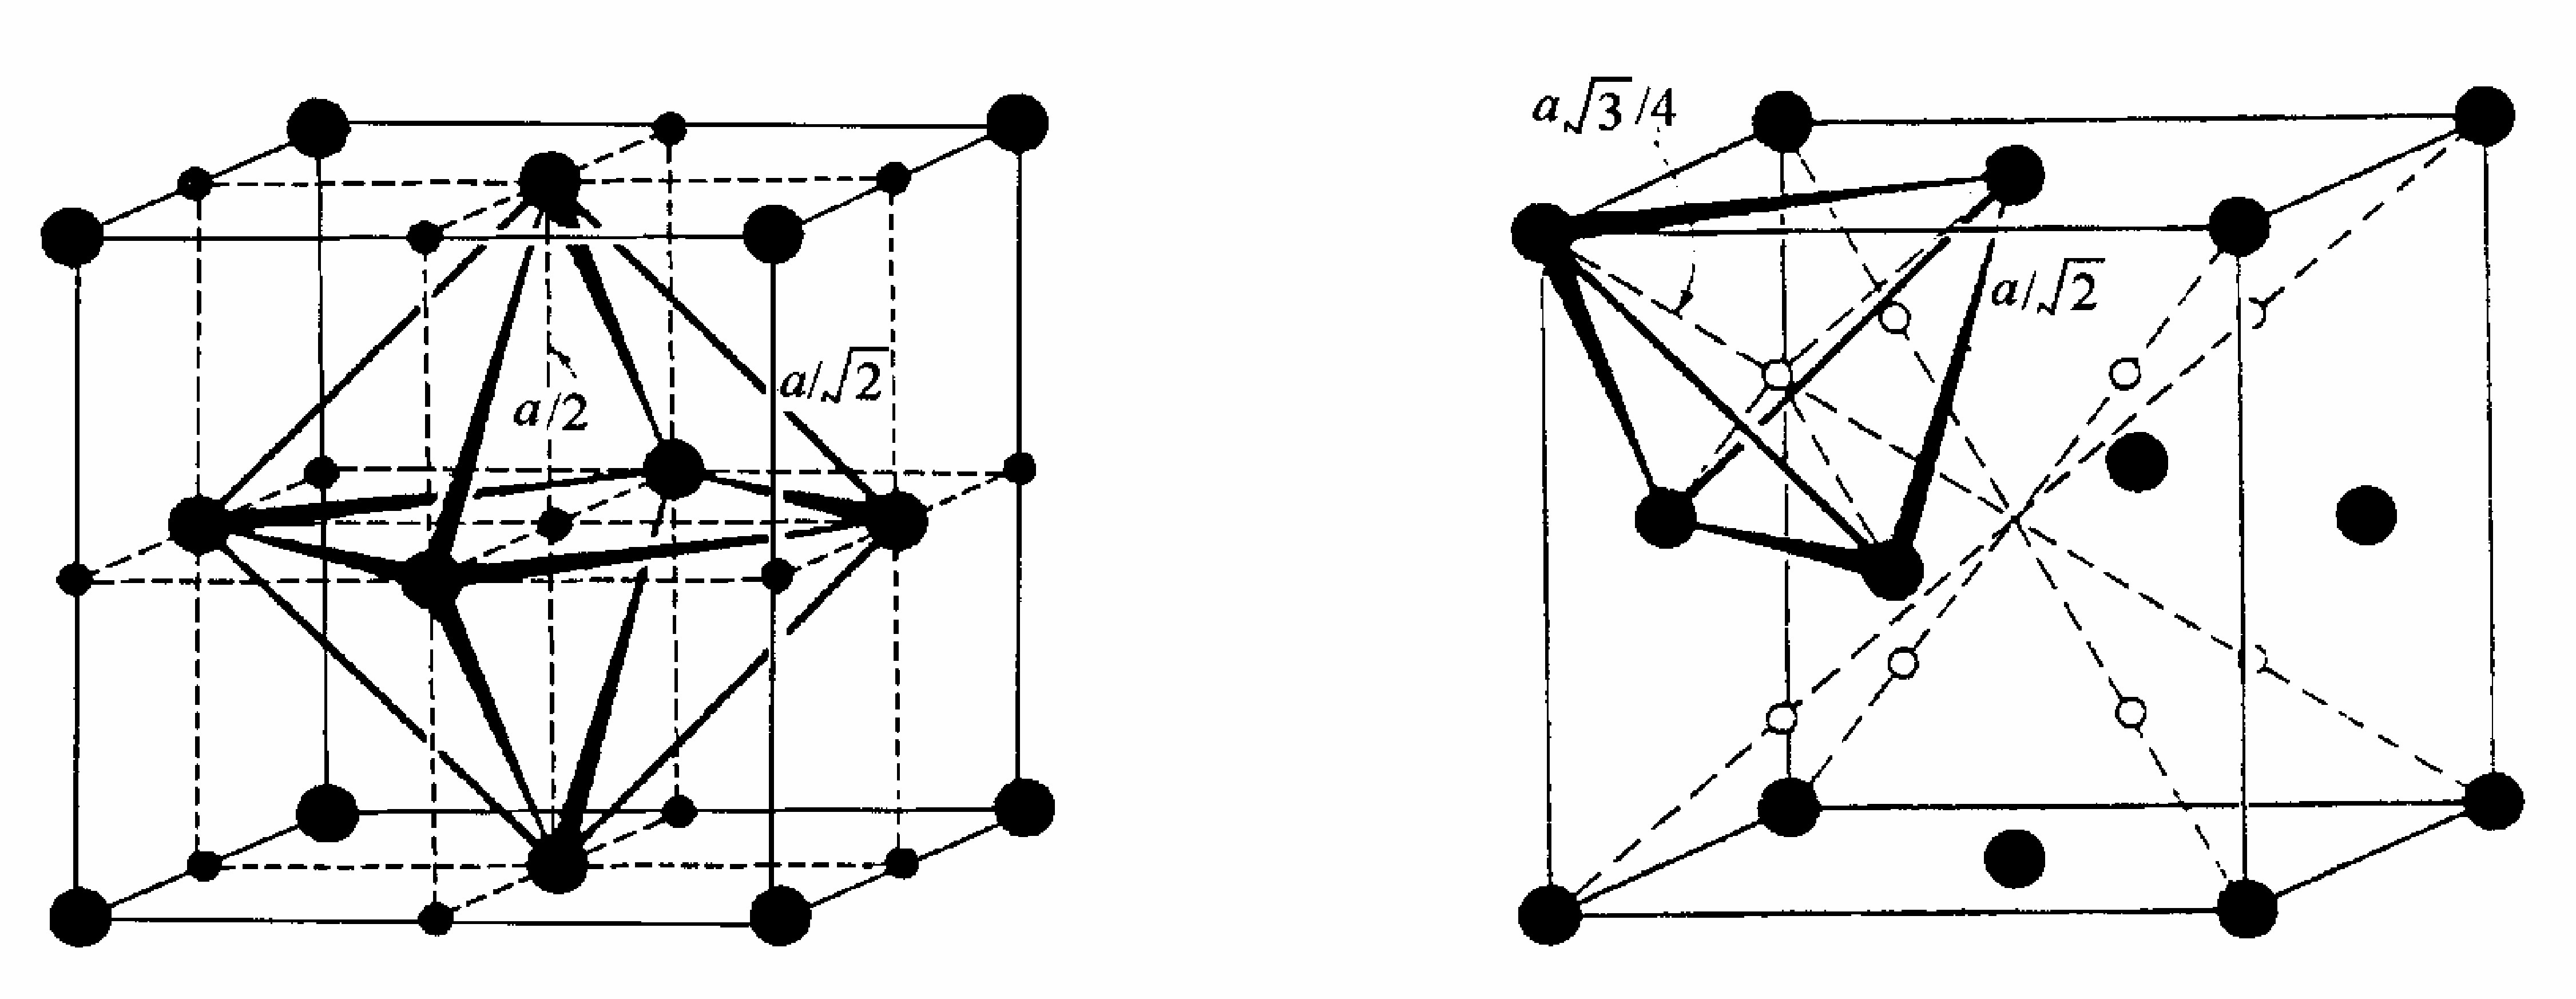
\includegraphics[scale=0.08]{Ch10/ClosestPacking/ccpvoid}
	\caption{Locations of interstices in hcp cells}
\end{figure}
%
\begin{table}
	\centering
	\begin{tabular}{@{}ll@{}}
		\toprule
		\ \textbf{Items}	& \textbf{Coordinates}										\\
		\midrule
		\ Atoms				& (0, 0, 0), (0, 1/2, 1/2), (1/2, 1/2, 0), (1/2, 0, 1/2)\ 	\\
		\ Octahedral Sites	& (0, 0, 1/2), (0, 1/2, 0), (1/2, 0, 0), (1/2, 1/2, 1/2)\ 	\\
		\ Tetrahedral Sites	& $(i/4,\,j/4,\,k/4),\ i,j,k\in\{1,3\}$\						\\
		\bottomrule
	\end{tabular}
	\caption{interstice sites in ccp}
	\label{ccpsite}
\end{table}\\
%
If the stacking does not strictly follow $ABCABC$, other structure with one 3, 
$\bar{3}$ or $3_1$, $3_2$ can be constructed. 
(At least a 3 is guaranteed though.) Examples are listed in table \ref{ccp3}.
%
\begin{table}
	\centering
	\begin{tabular}{@{}ll@{}}
		\toprule
		\ \textbf{Symmetry}	& \textbf{Stacking Unit}\	\\
		\midrule
		\ $3$				& $ABACB$					\\
		\ $\bar{3}$			& $ACBAB$					\\
		\ $3_1$				& $ABCBCACAB$\ 				\\
		\bottomrule
	\end{tabular}
	\caption{Stackings with 3}
	\label{ccp3}
\end{table}
%
\subsection{Other Packings}
%
The space effeciency of closest packings can be calculated:
%
\[
	\eta=\frac{4\cdot4\pi r^3/3}{(2\sqrt{2}r)^3}\approx 74.05\%
\]
%
For closest pack layers, if two same layers stack together, 
trigonal prismatic interstices $a+b$, whose number is twice that of atoms will occur.\\
Another looser but common packing paradigm is body-centered cubic packing (bcc), whose space effeciency is:
%
\[
	\eta=\frac{2\cdot4\pi r^3/3}{(4r/\sqrt{3})^3}\approx 68.02\%
\]
%
\section{Structure of Metallic Solids}
%
\subsection{Pure Metals}
%
Almost all pure metals take forms among hcp, ccp and bcc except Po which is $cP$. 
Figure \ref{metals} shows the lattice type of all metals at room temperature:
%
\begin{figure}[h]
	\centering
	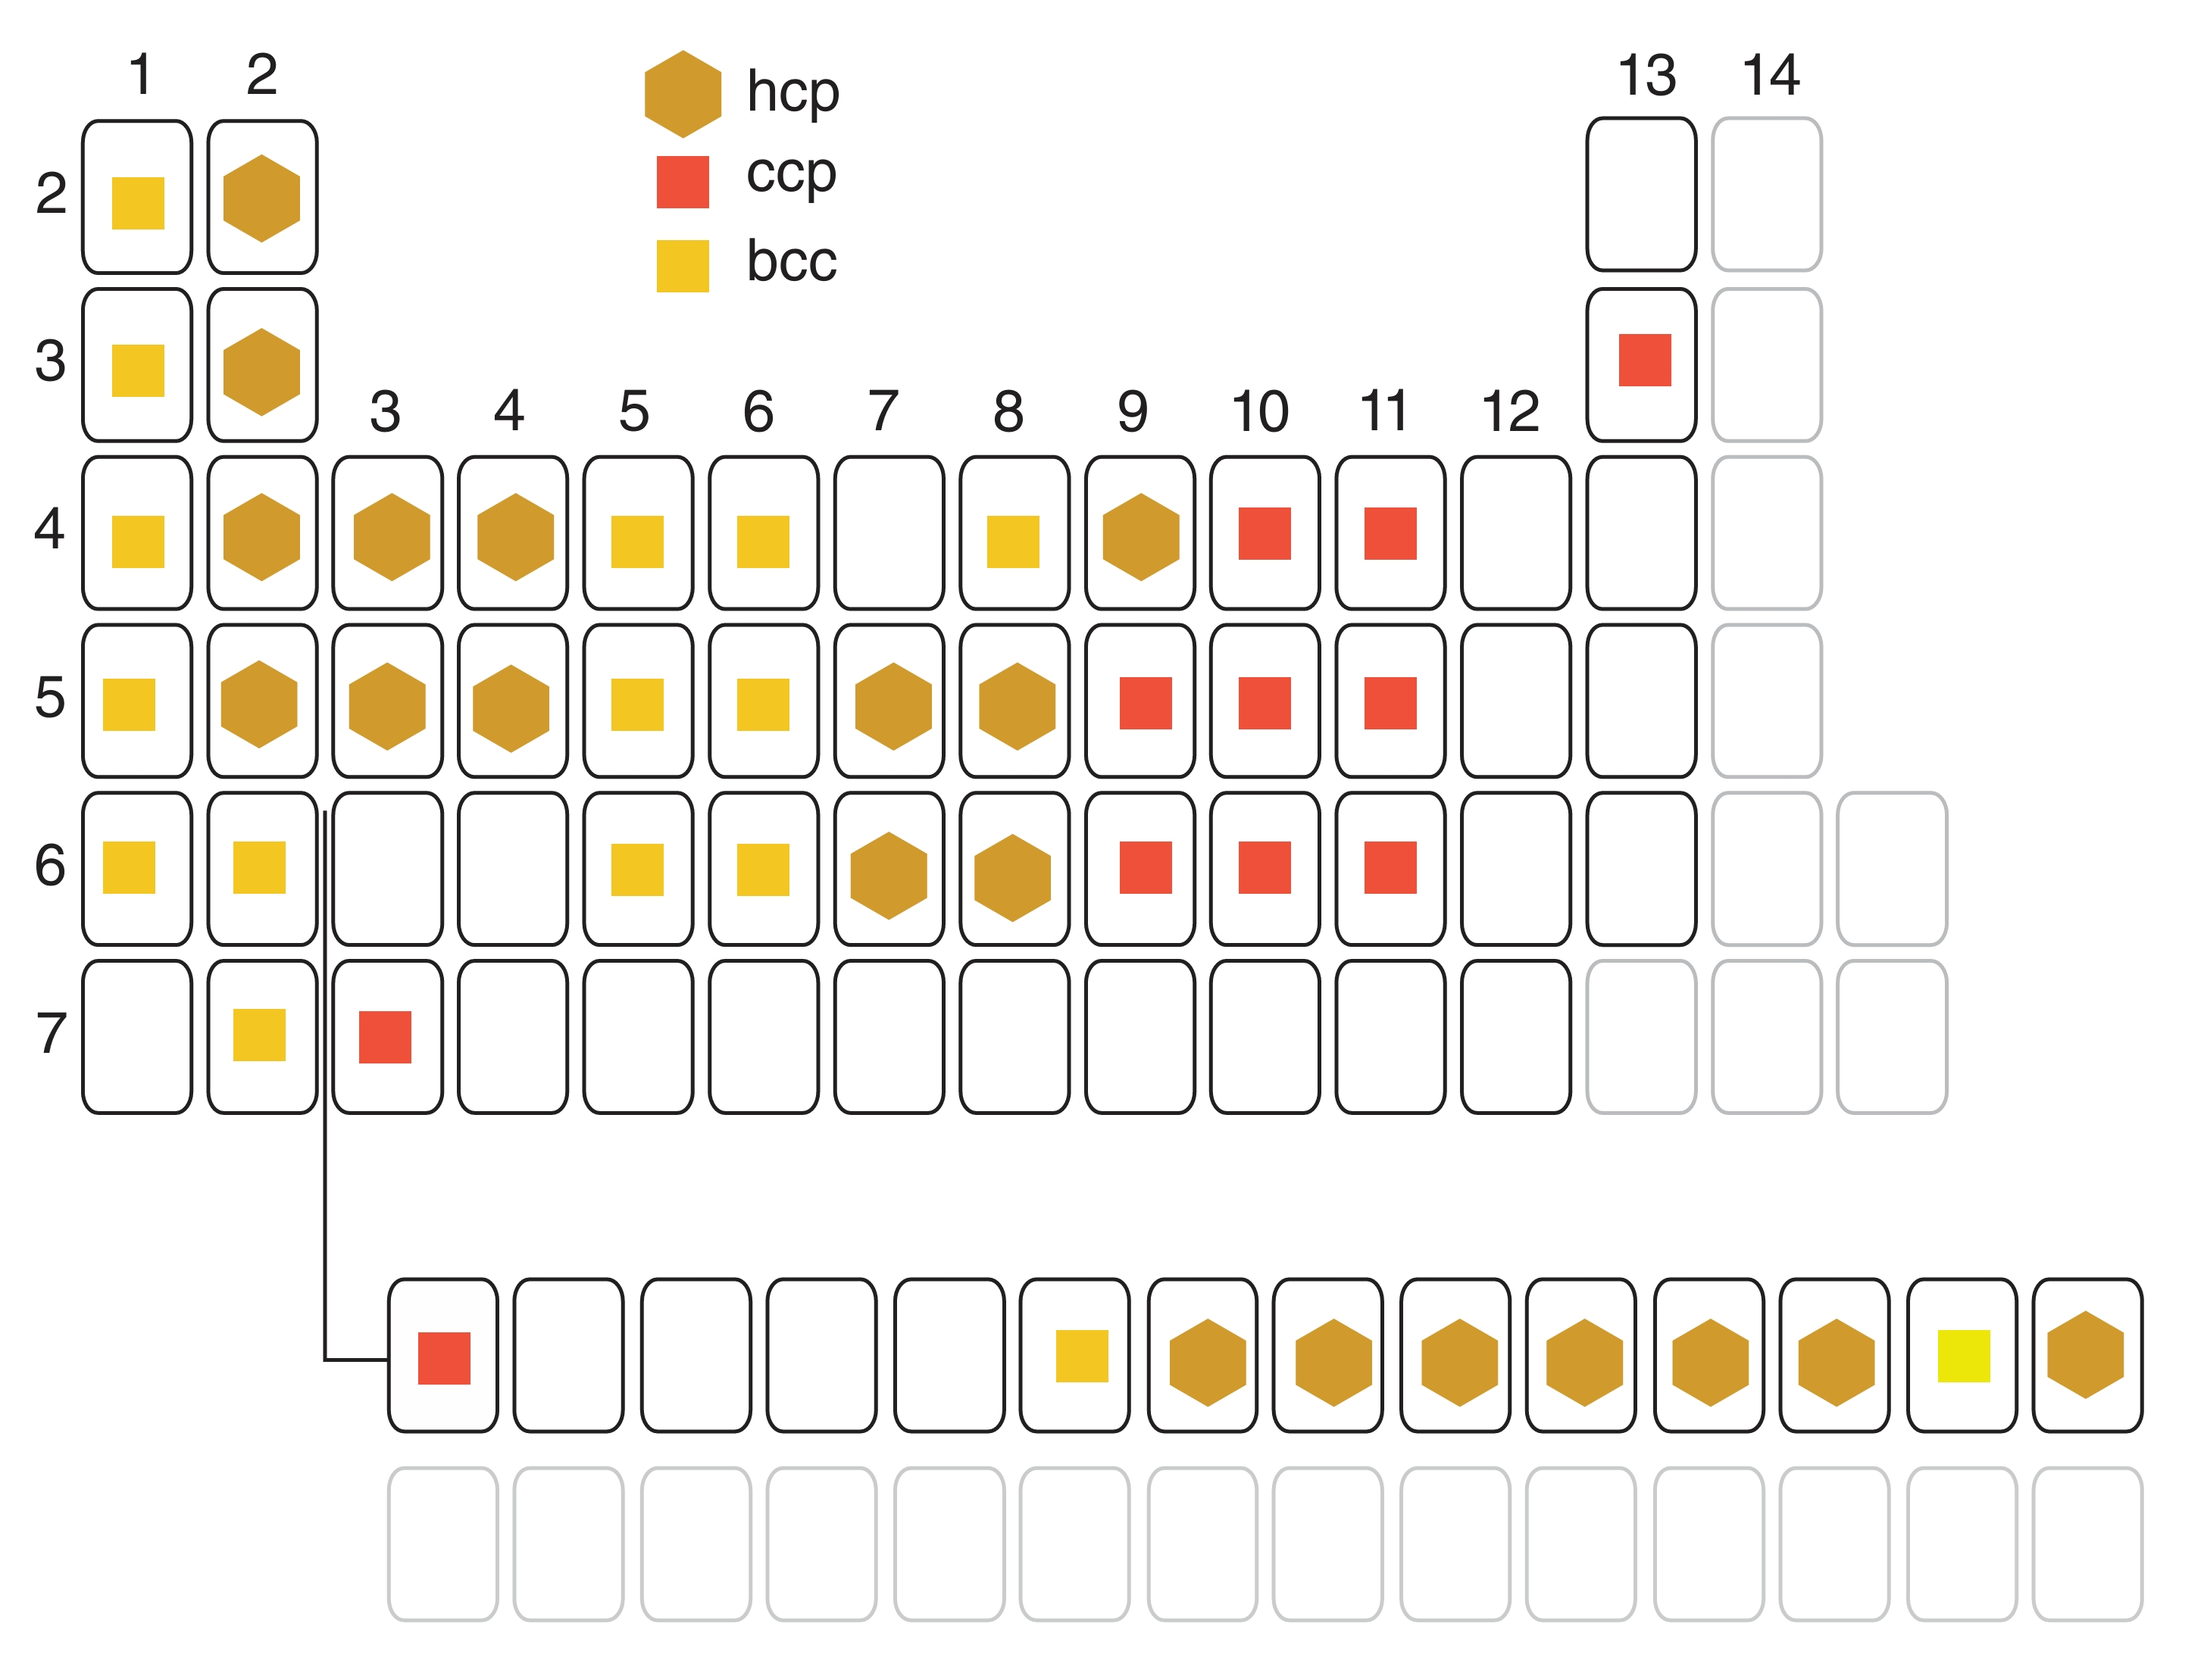
\includegraphics[scale=0.1]{Ch10/Lattice/metals}
	\caption{Lattice tpye of metals at room temperature}
	\label{metals}
\end{figure}
%
Since ccp stacking can be seen from four directions but hcp only one, 
metals that stack in ccp mode are often more malleable than hcp ones.
Also due to entropy effects, real metals rarely exhibit perfect $ABC$ stacking; 
stacking faults and mixed sequences are common, and as long as nearby layers aren't the same, it is still closest packing.
This phenomenon is called polytypism of metals.\\ \\
%
Besides, metals change crystal structure with $p$ and $T$ due to thermal motion, namely polymorphism
At low $p$ and high $T$, every metal atoms want more space to vibrate, so a less dense packing pattern, often bcc, is adopted.
For most metals, this transition occurrs higher than room temperature, but alkali metals are the exceptions.
%
\subsection{Alloys}
%
The components of alloys don't all have to be metals, and alloy itself don't have to be a mixture.
As long as the resulting substance exhibits metallic properties it can be regarded as an alloy.
Generally alloys can be classified into three categories:
%
\subsubsection{Interstitial Alloys}
%
Interstitial alloys form when small atoms (H, B, N, C) occupy the interstices of a host metal without electron transfer. 
There is either a simple whole-number ratio of metal and interstitial atoms (as in tungsten carbide, WC) 
or the small atoms are distributed randomly in the available spaces between the packed atoms (as in pig iron, Fe(C)).
The interstitial atoms squeeze themselves in, increasing stress in the lattice, 
which results in enhanced hardness but a more brittle character.\\
Carburizing process utilizes this principle to harden wrought iron.
%
\subsubsection{Substitutional Alloys}
%
Substitutional alloys involves the replacement of one type of metal atom in a structure by another, 
retaining the original lattice structure. These are generally formed if three criteria are fulfilled:
%
\begin{itemize}
	\item The atomic radii of the elements are within about 15 per cent of each other;
	\item The crystal structures of the two pure metals are the same, similar metal-metal interactions;
	\item The electropositive characters of the two components are similar, no electron transfer.
\end{itemize}
%
Ni-Cu system is a good example for this: neighbors, both ccp, radii 125 pm and 128 pm.
They form fully miscible solid solutions ranging from pure nickel to pure copper.
%
\subsubsection{Intermetallic Compounds}
%
When some liquid mixtures of metals are cooled, 
they form phases with definite structures that are often unrelated to the parent structure. 
These phases with exact stoichiometry are called intermetallic compounds, though the stoichiometry might be complicated.
Due to the regular alignment of different metals in the lattice, 
intermetallic compounds are normally high-melting, hard, and more brittle than most metals and alloys.\\ \\
%
A Zintl phase is described when a very electropositive metal and a less electropositive metal/metalloid form intermetallic compounds.
Partial electron transfer may take place and they are often described as metal (cluster) cations or anions though not fully ionic.
%
\section{Structure of Ionic Solids}
%
\subsection{General Description of Ionic Solids}
%
The ionic model treats an ionic solid as an assembly of oppositely charged, hard spheres 
that interact primarily by nondirectional electrostatic forces (Coulomb interactions). 
As anions which gain electrons generally have larger radii compared to cations that lose them, 
these structures are often described as cations filling the interstice sites in anion stackings.\
Table \ref{ionicstructure} listed some of them
%
\begin{table}
	\centering
	\begin{tabular}{@{}lll@{}}
		\toprule
		\ \textbf{Lattice Type}	& 	\textbf{Anion Packing} 			&	\textbf{Cation Filling}							\ \\
		\midrule
		\ Halite				&	ccp								&	All octahedral									\ \\
		\ Antifluorite			&	ccp								&	All tetrahedral									\ \\
		\ Sphalerite			&	ccp								&	Half tetrahedral								\ \\
		\ Spinel				&	ccp								&	Half octahedral and 1/8 tetrahedral 			\ \\
		\ Wurtzite				&	hcp								&	Half tetrahedral								\ \\
		\ Corundum				&	hcp								&	2/3 octahedral									\ \\
		\ Rutile				& 	hcp (distorted)					&	Half octahedral									\ \\
		\ $\rm NiAs$			&	hcp								&	All octahedral									\ \\
		\ $\rm CdCl_2$			&	ccp								&	Half octahedral									\ \\
		\ Perovskite			&	Joint ccp or hcp by A and X 	&	All octahedral formed by X 						\ \\
		\bottomrule
	\end{tabular}
	\caption{Staking-Filling model for ionic lattice types}
	\label{ionicstructure}
\end{table}
%
\subsection{Halites and Cubic Perovskites}
%
In halite structure, anions stack as ccp and cations fill all the octahedral sites, 
so it's also fine to say anions fill all the octahedral sites formed by cation ccp. 
If anions aren't spherical and are oriented along one lattice axis, 
say the rod-shaped acetylides $\rm C_{2}^{2-}$ along $c$,
the lattice would then elongate in that direction, 
keeping one 4-fold axis while losing the 3-folds, downgrading to $tI$.
Figure \ref{halite} illustrates the two structures.\\
%
\begin{figure}[h]
	\centering
	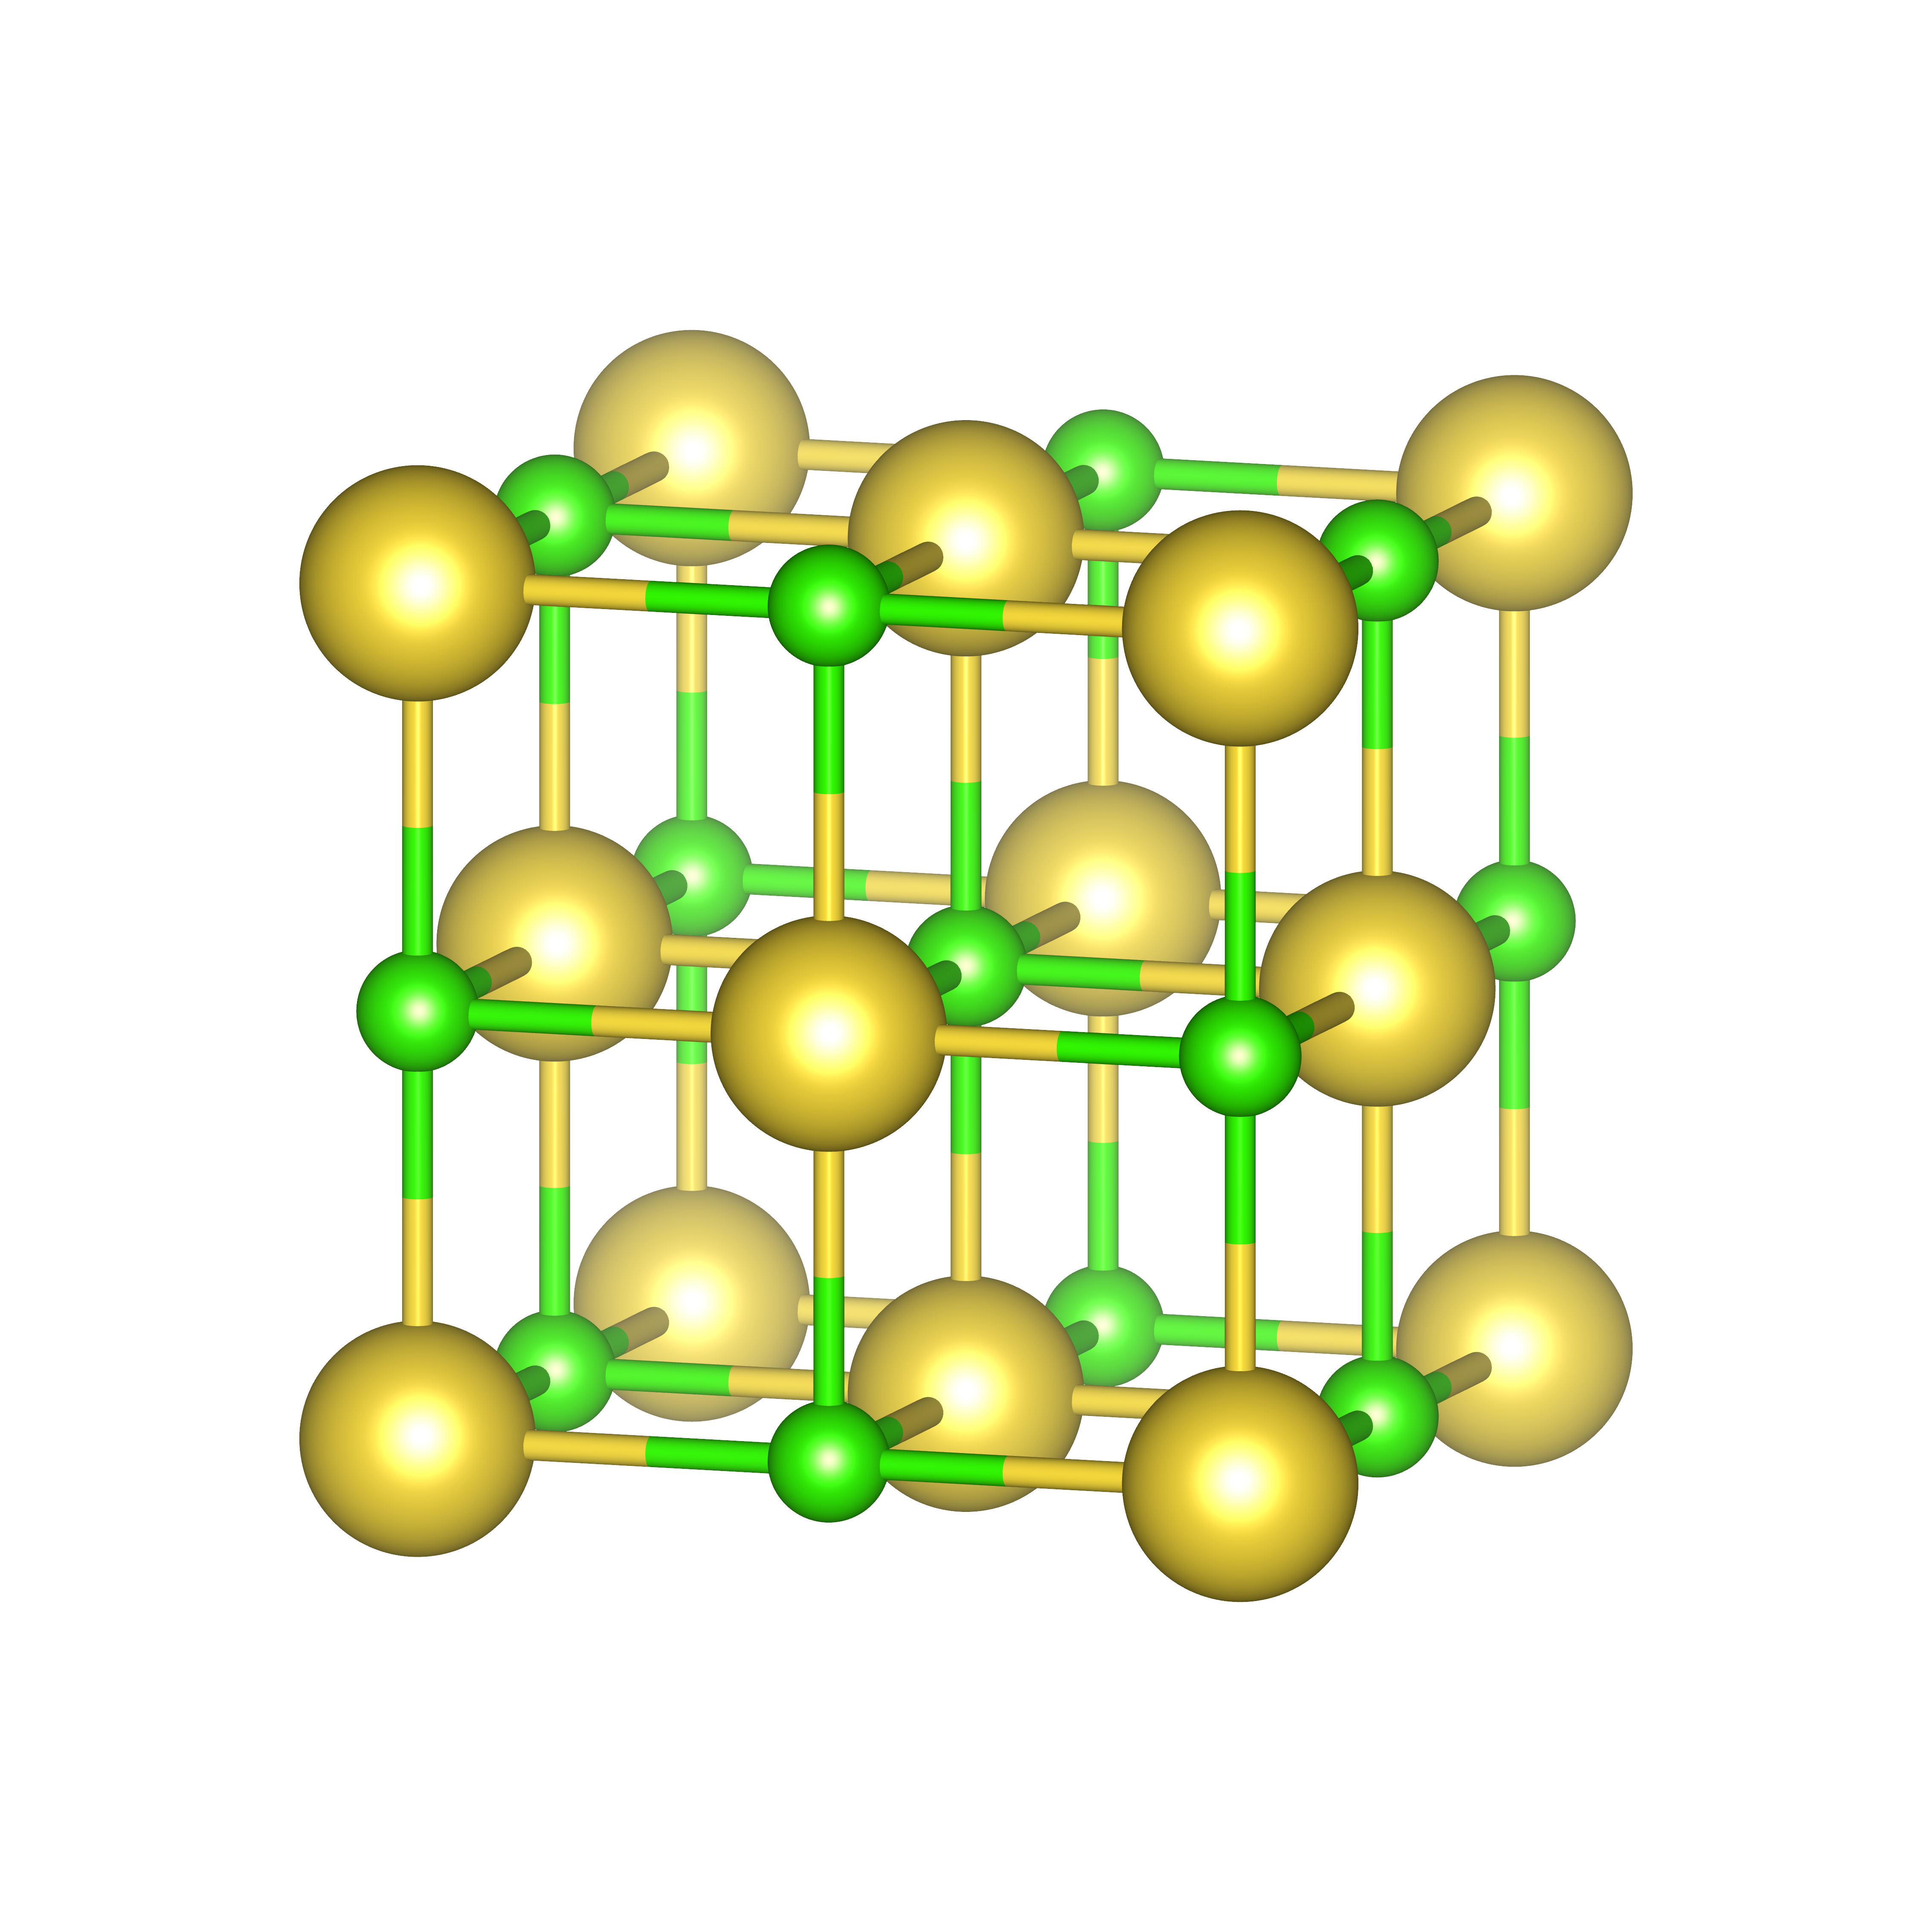
\includegraphics[scale=0.04]{Ch10/Halite/NaCl}
	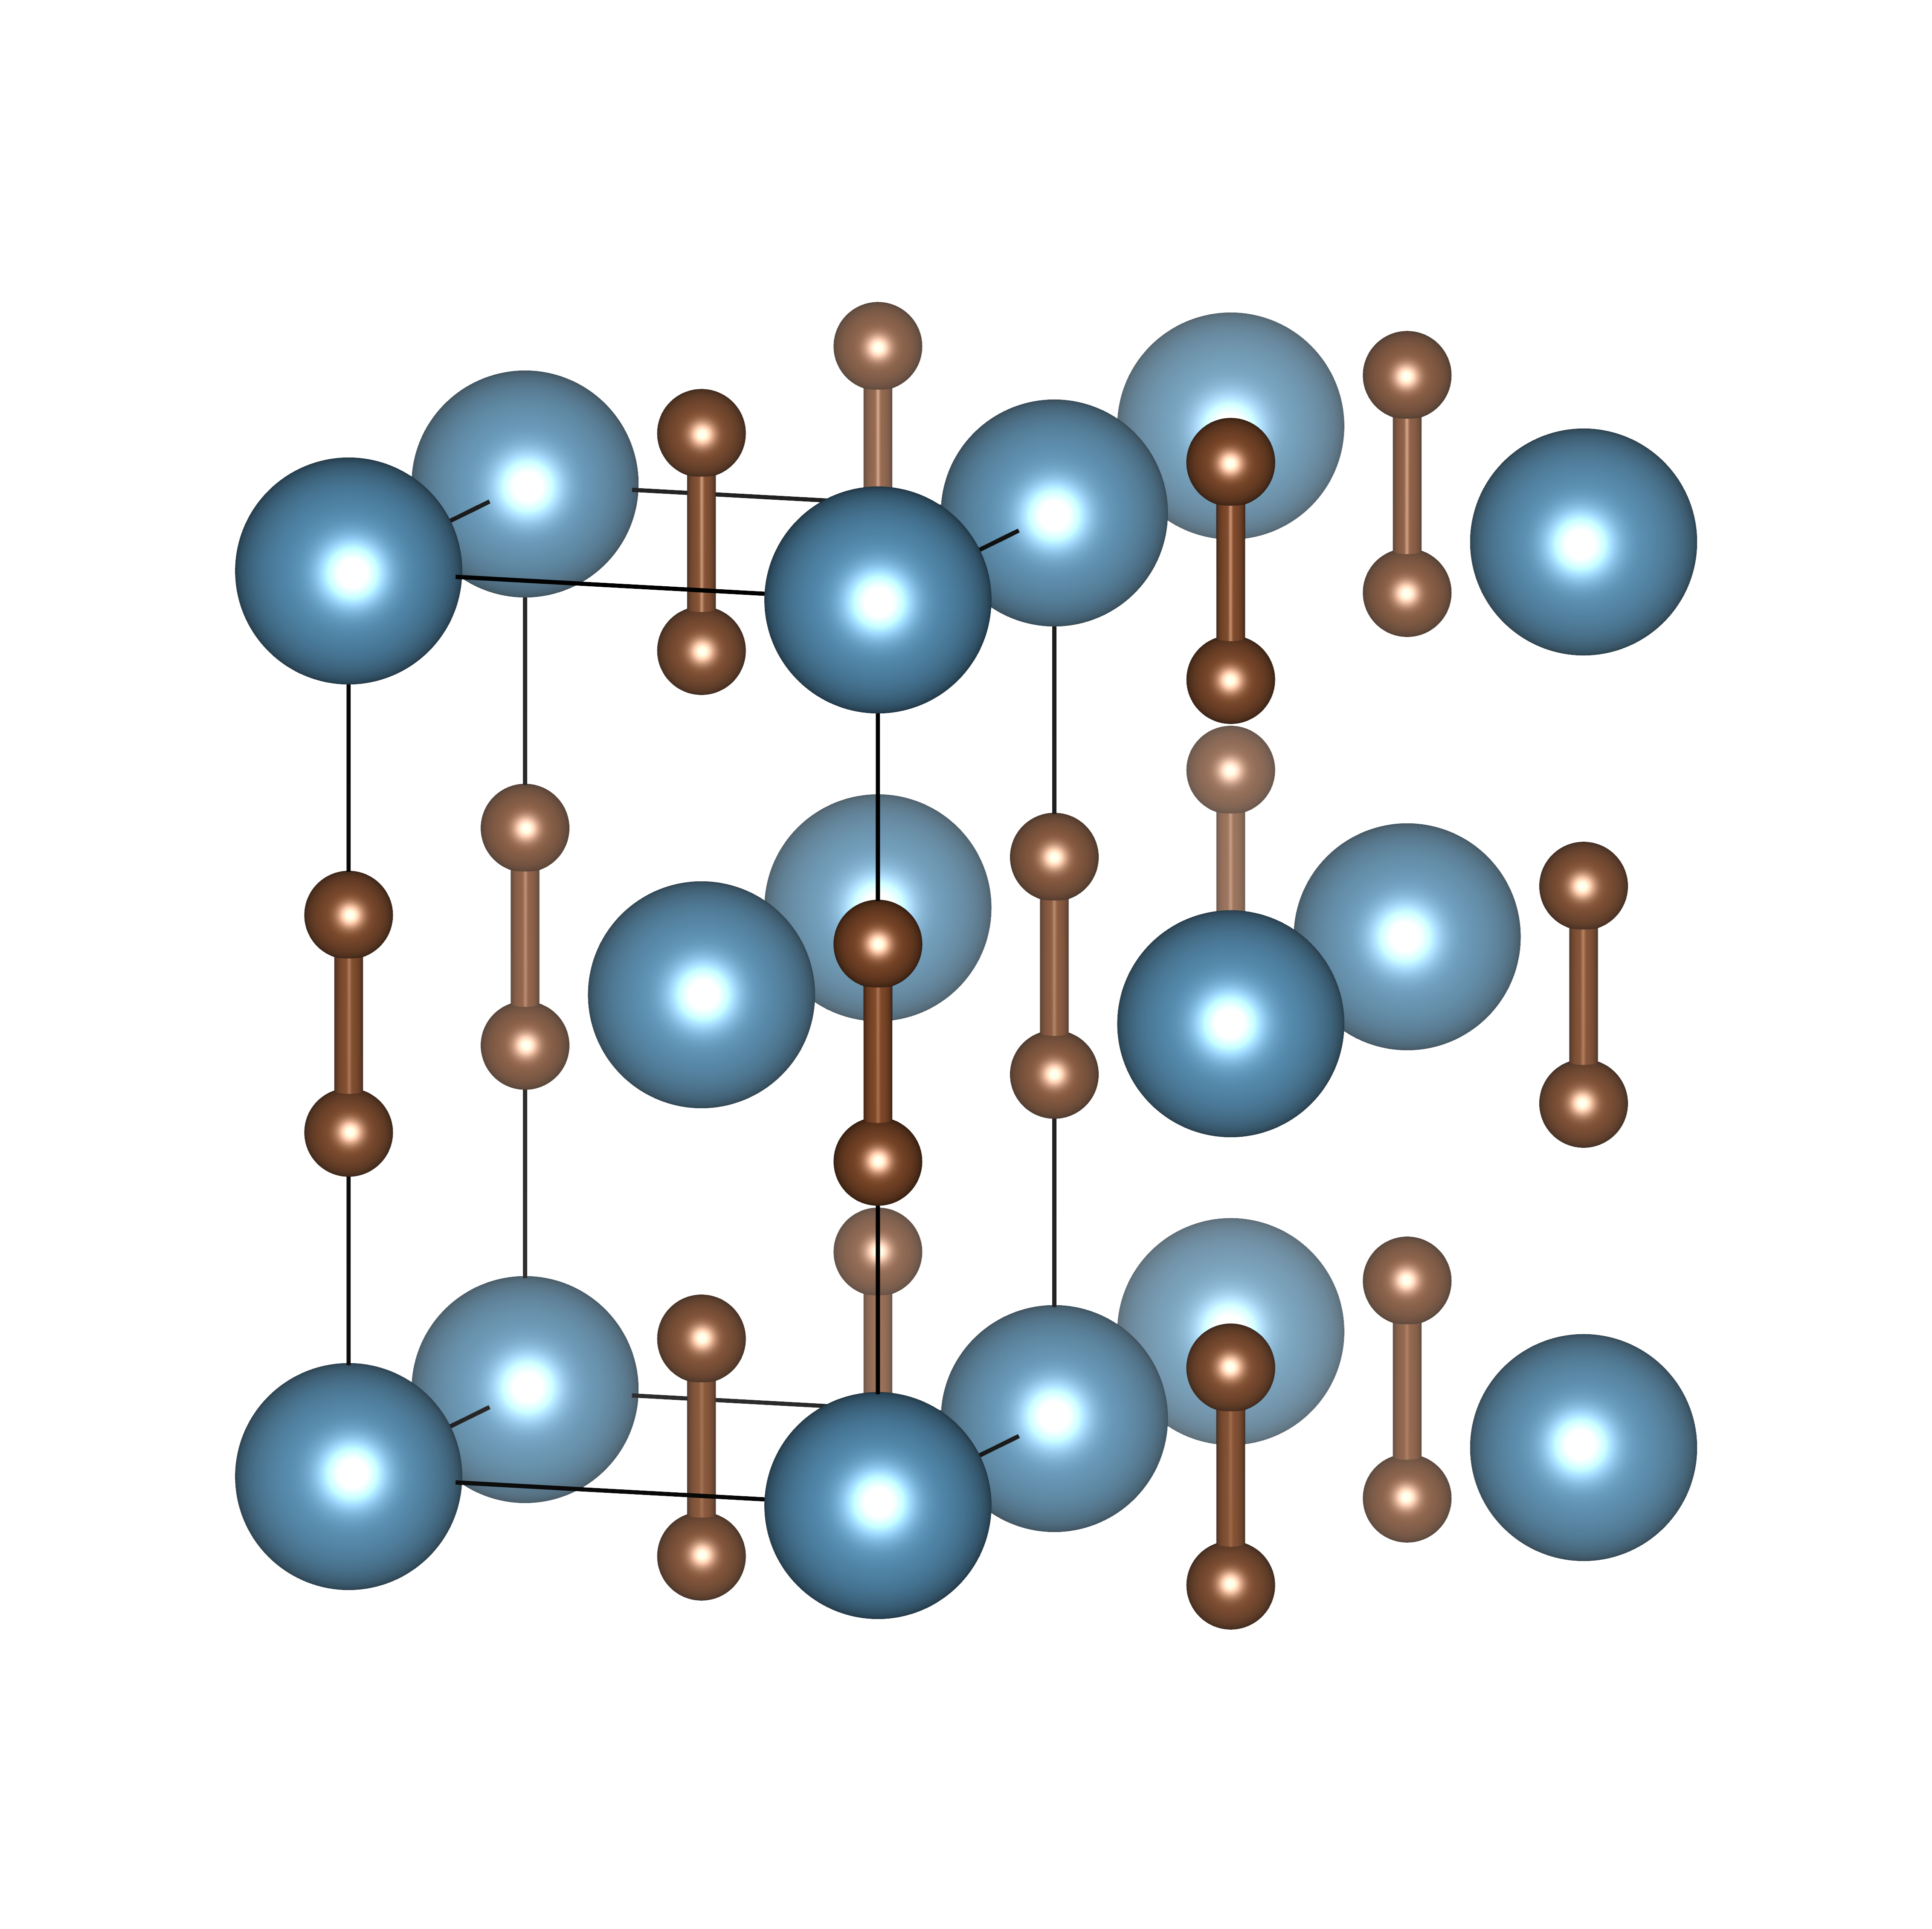
\includegraphics[scale=0.04]{Ch10/Halite/CaC2}
	\caption{Halite-type lattice structure}
	\label{halite}
\end{figure}\\
%
If we want to preserve the 3-fold axes at the cost of 4-folds, as in pyrite $\rm FeS_2$, 
we can place $\rm S_2^{2-}$ at vertices and face centers. 
Make all $\rm S_2^{2-}$s at the vertices orient along one body diagonal, 
and the ones at opposite faces along the same one of the other three body diagonals. 
Now the 4 3-fold axes are kept but no longer along 4 body diagonals. They are now along the bonding direcction of $\rm S_2^{2-}$. 
Each S is 4-coordinated (1S + 3Fe). Figure \ref{fes2} shows this structure and its 3-fold axis.\\
%
\begin{figure}[h]
	\centering
	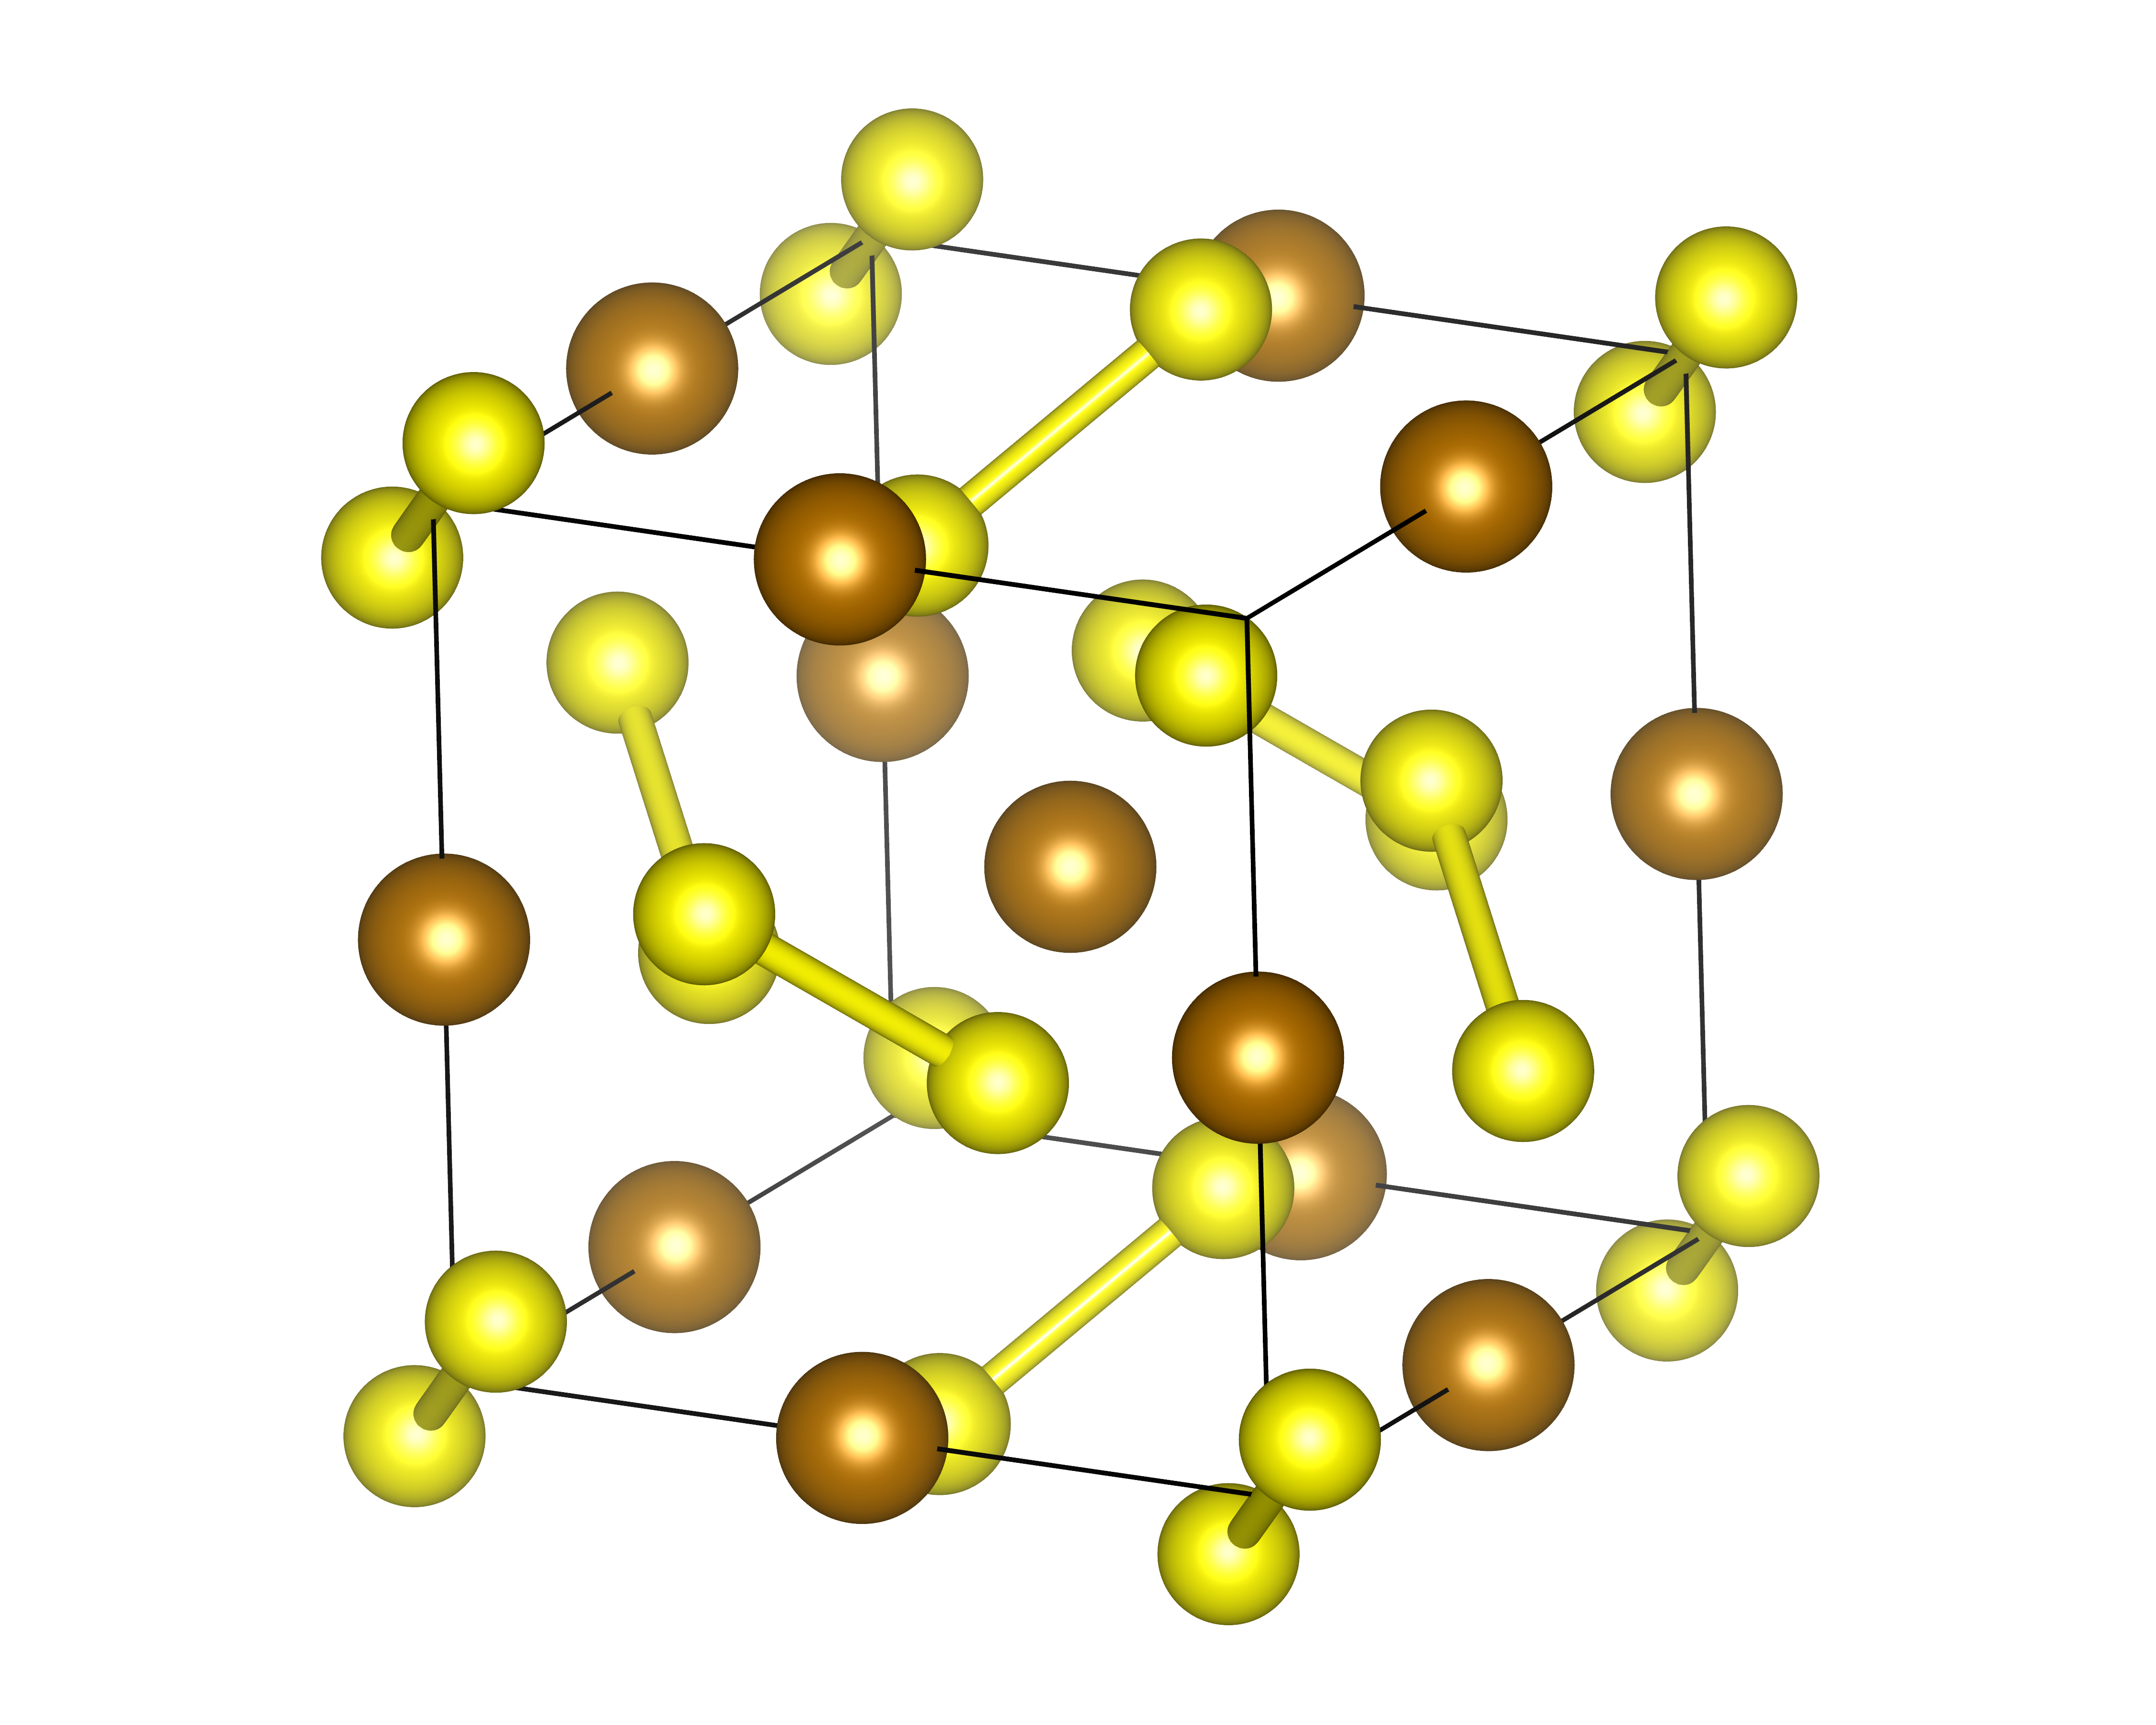
\includegraphics[scale=0.04]{Ch10/Halite/FeS2}
	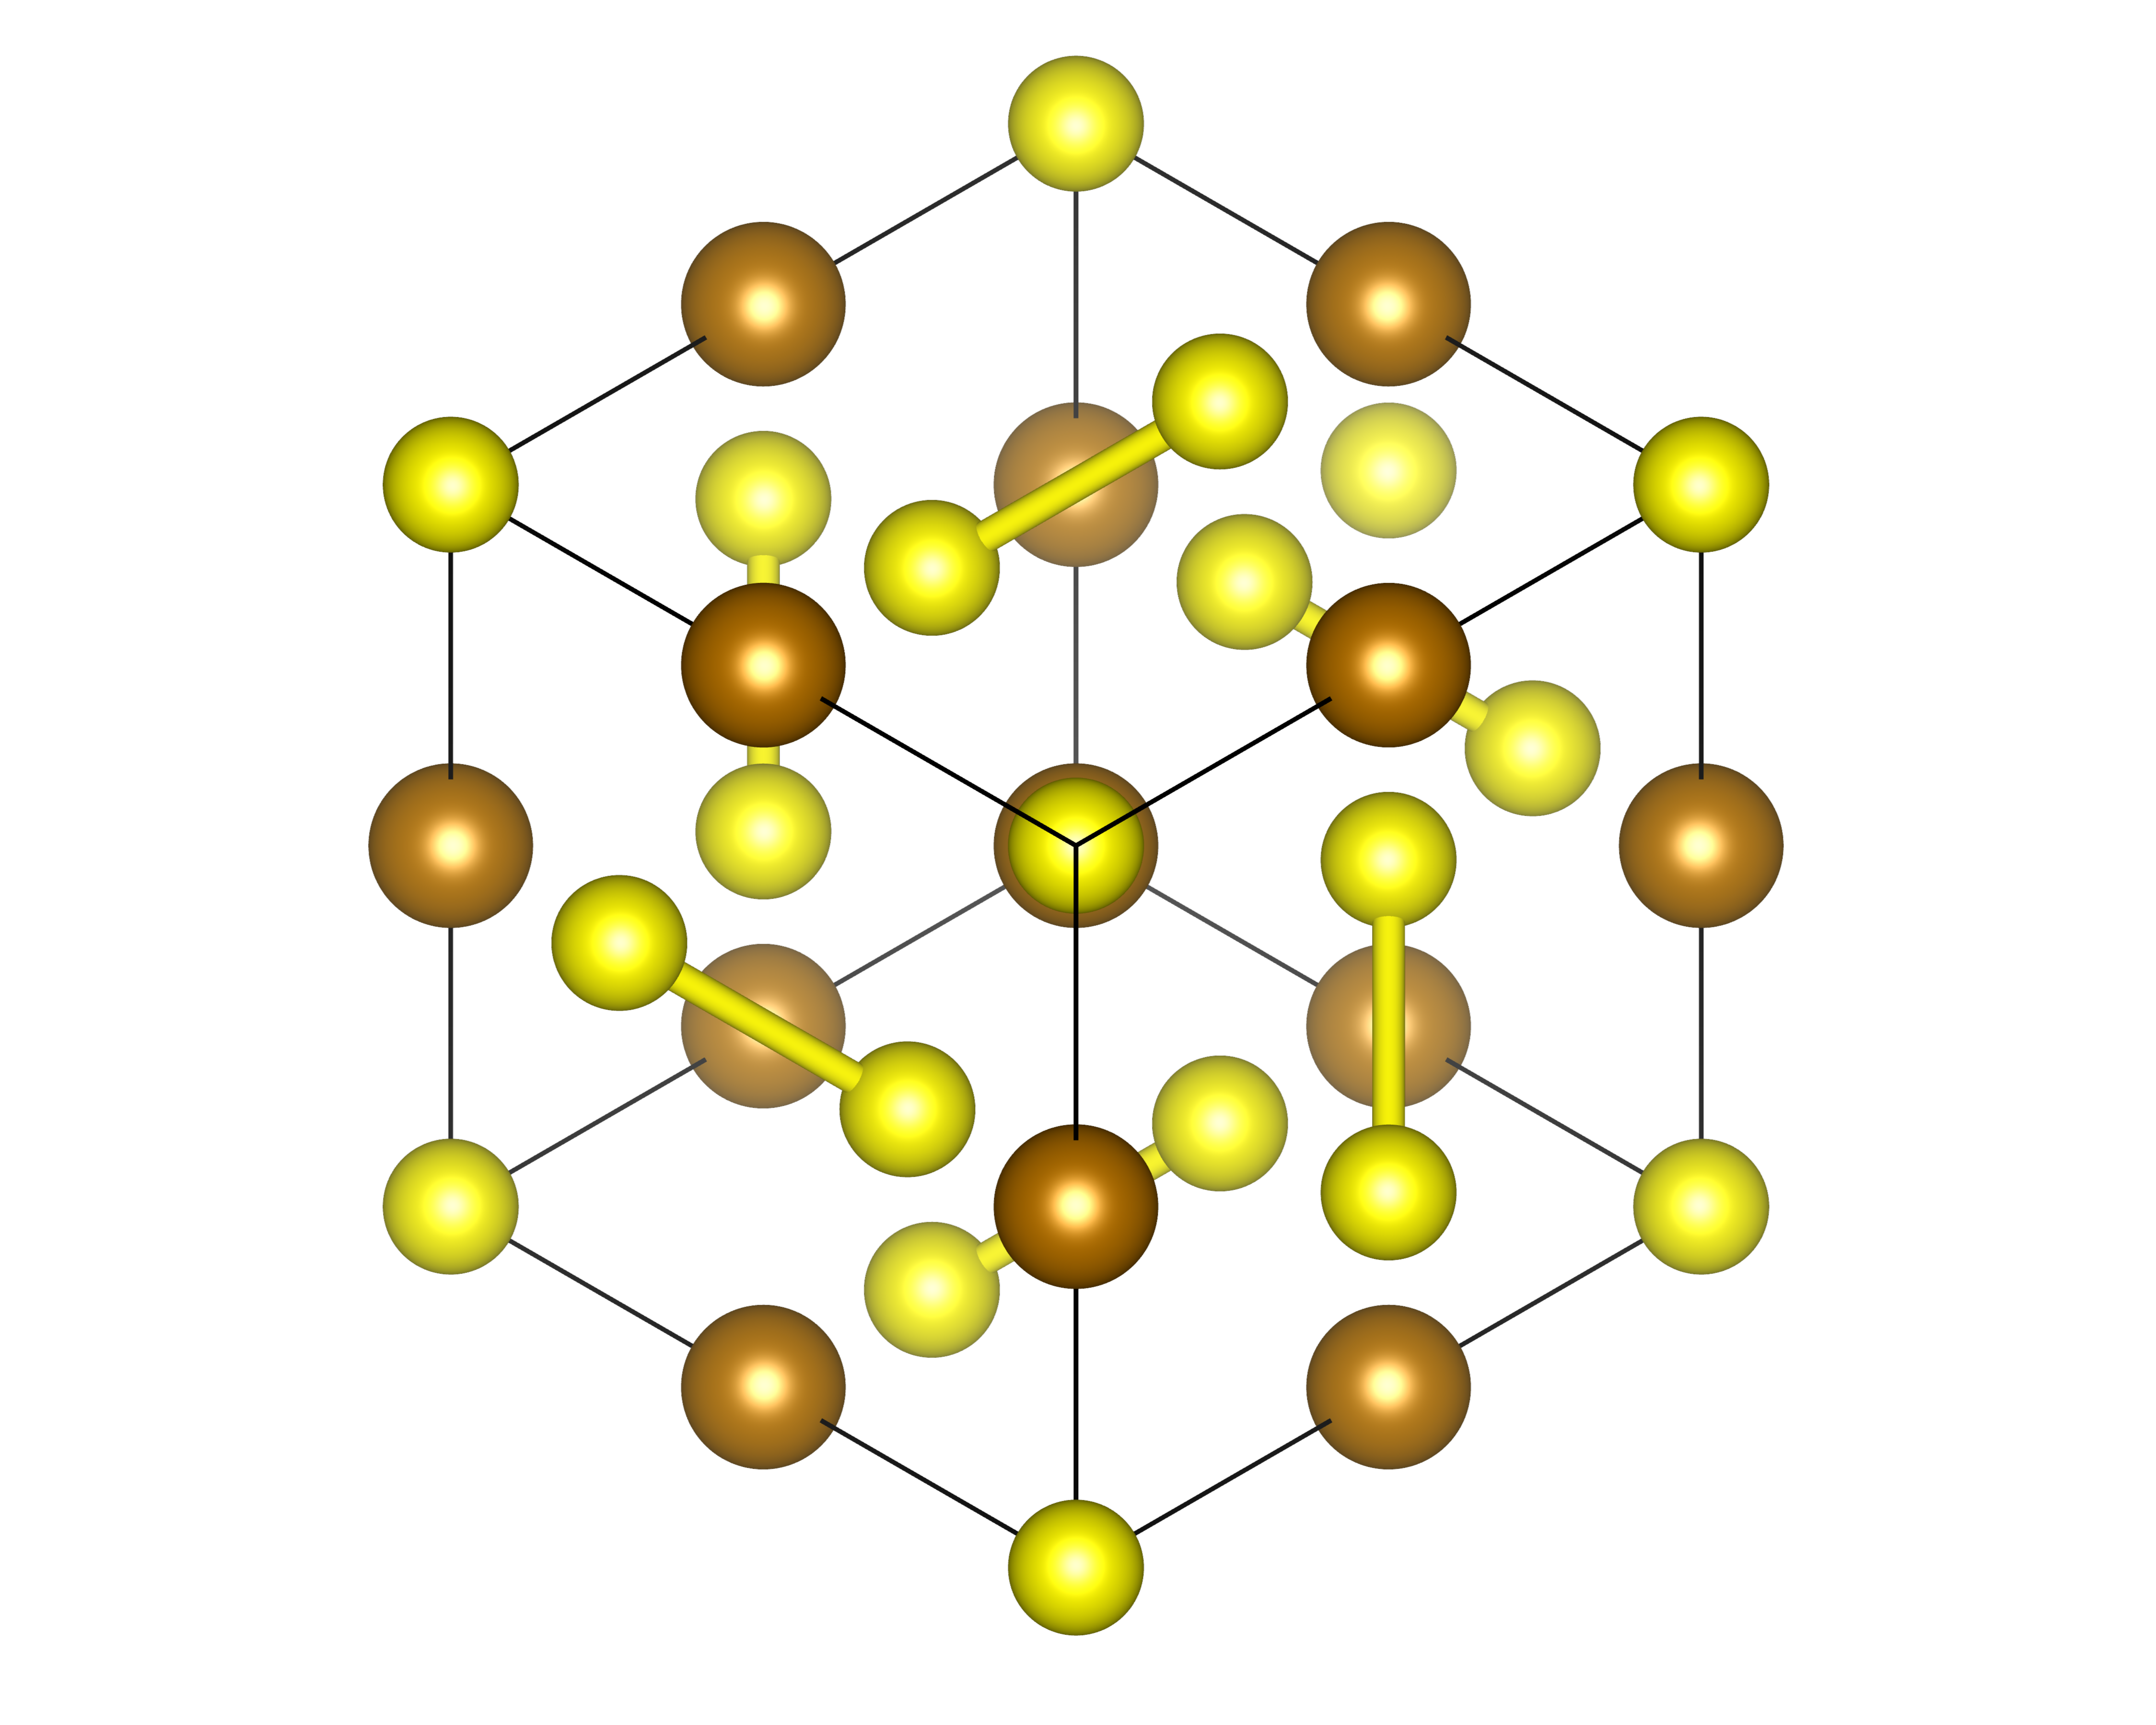
\includegraphics[scale=0.04]{Ch10/Halite/FeS2_3}
	\caption{Unit cell of pyrite}
	\label{fes2}
\end{figure}\ \\
%
More lattice structure can be derived from simple halite structure.
If we remove atoms at vertices and body center, we arrive at $\rm NbO$ structure;
if we remove atoms at body- and face centers, we arrive at $\rm ReO_3$ structure.
These two structures are shown in figure \ref{ReO3}.\\
%
\begin{figure}[h]
	\centering
	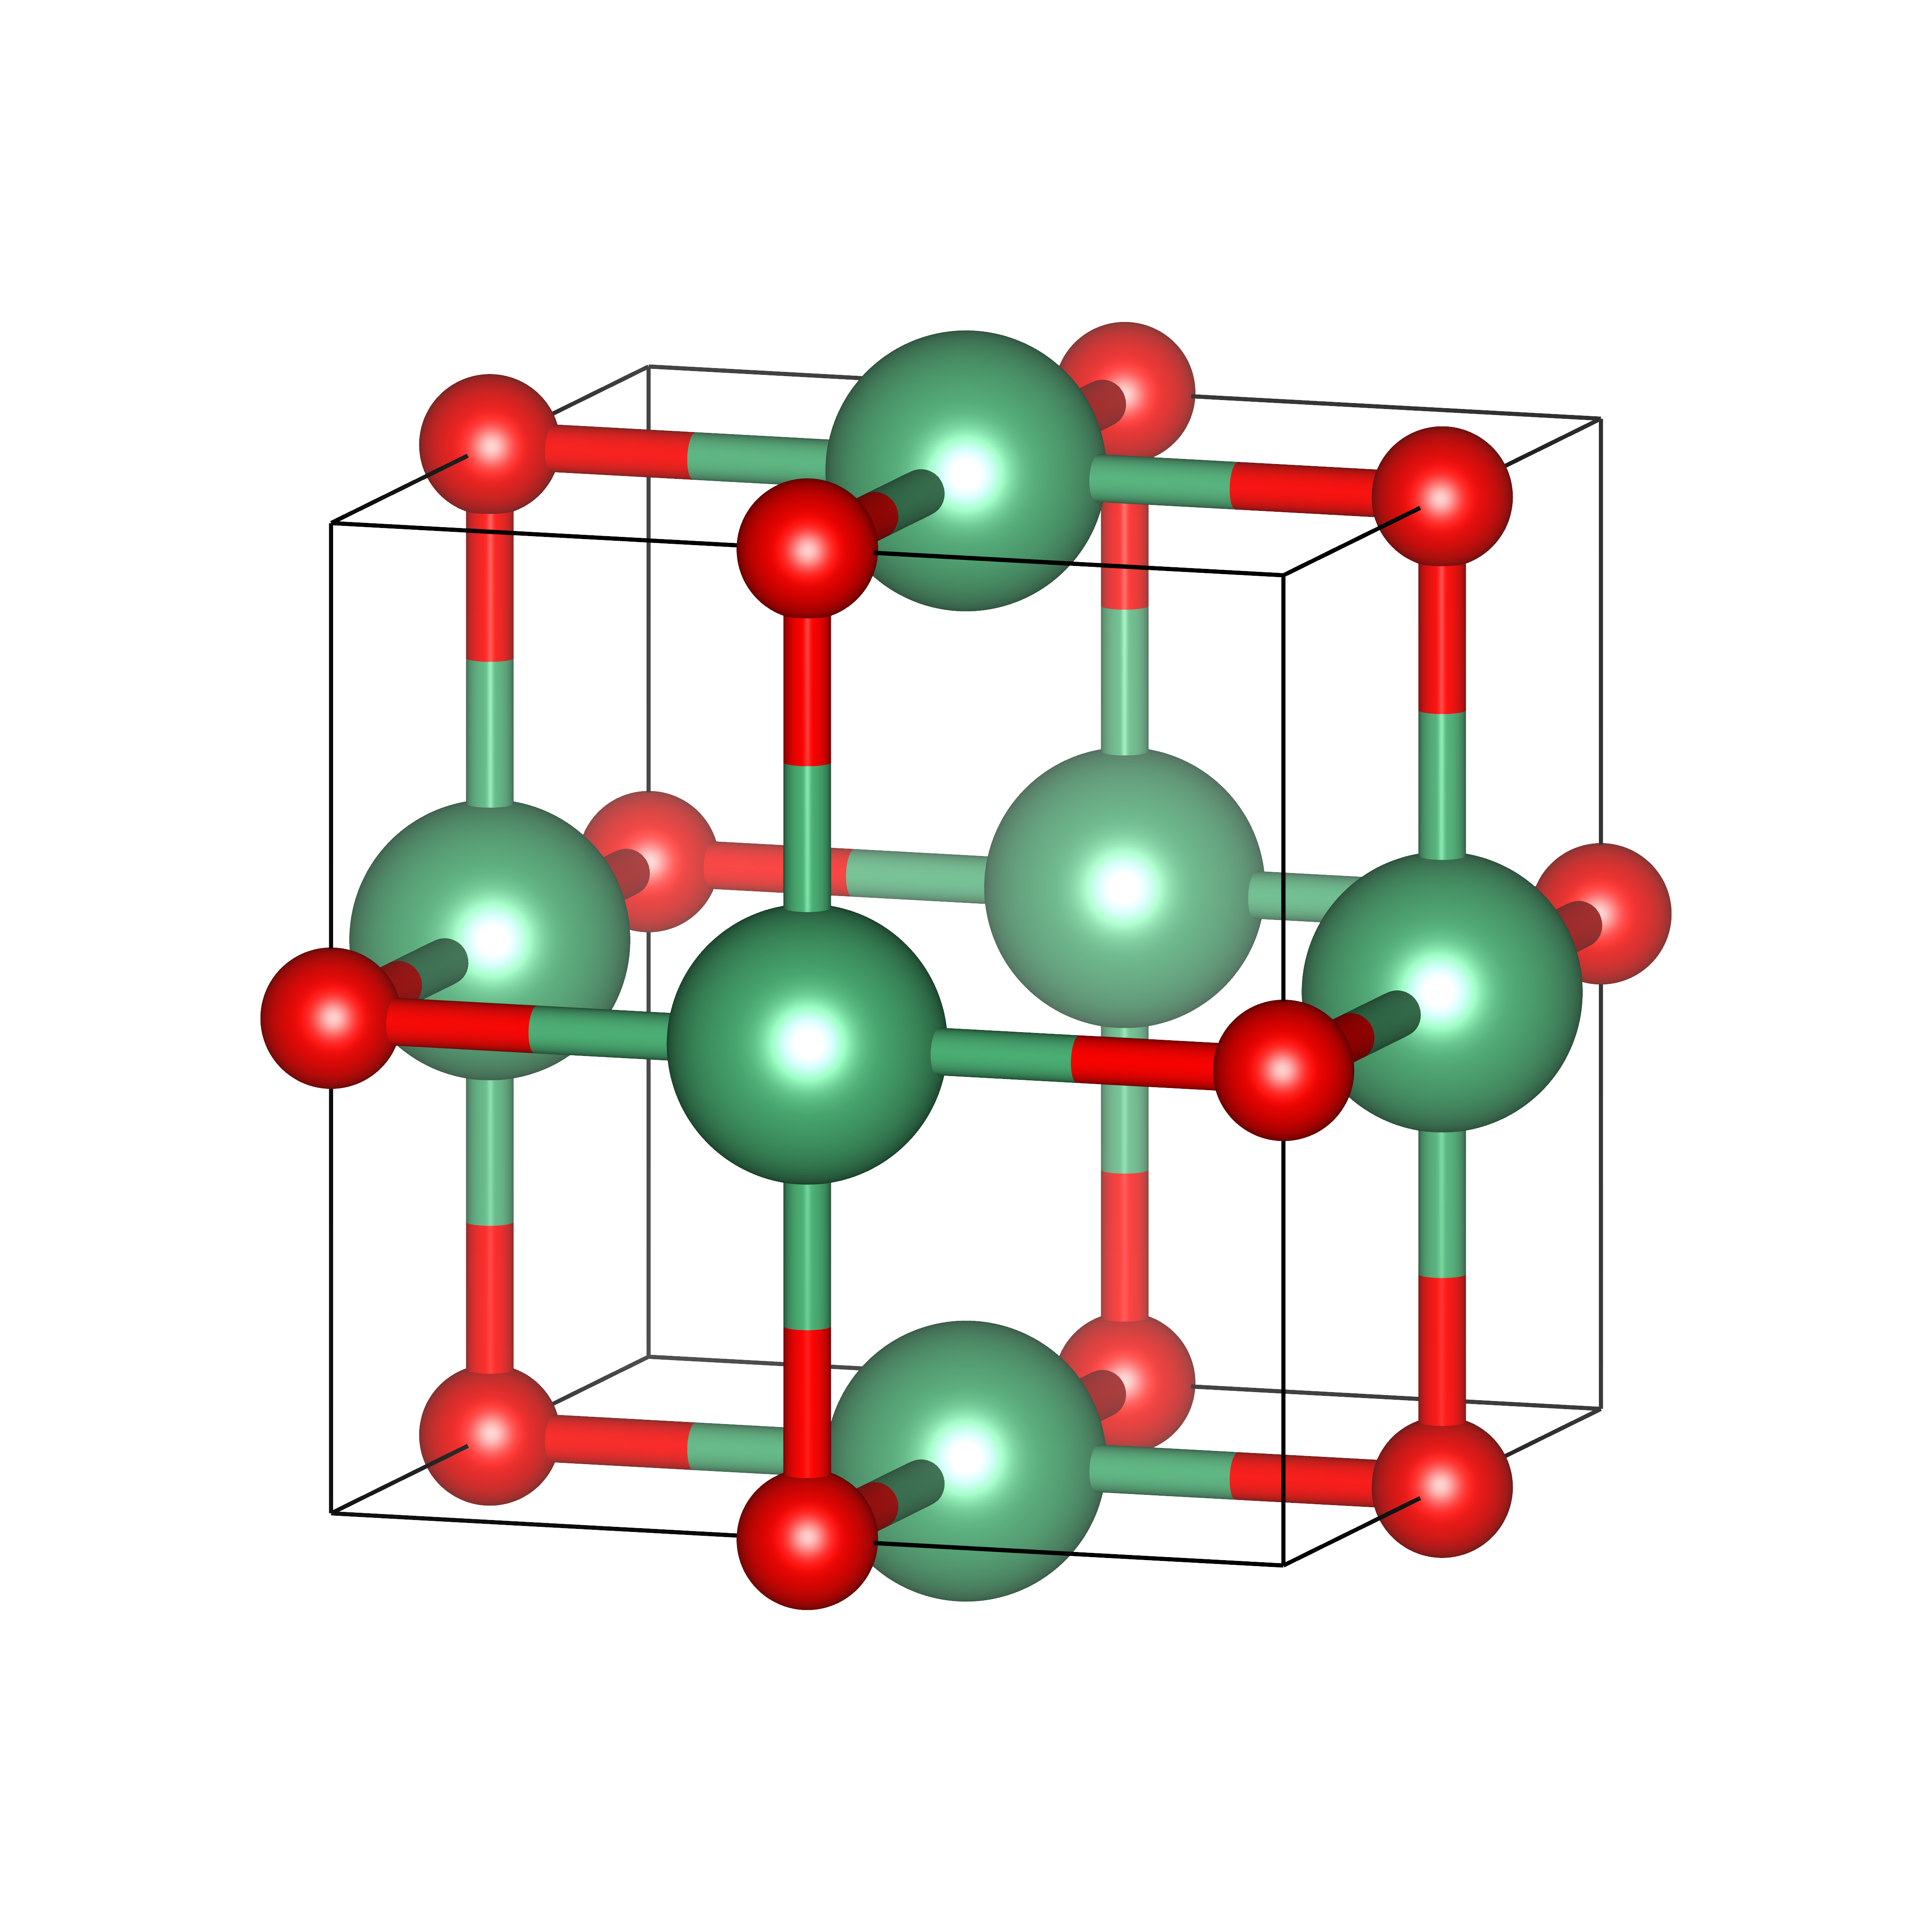
\includegraphics[scale=0.04]{Ch10/Halite/NbO}
	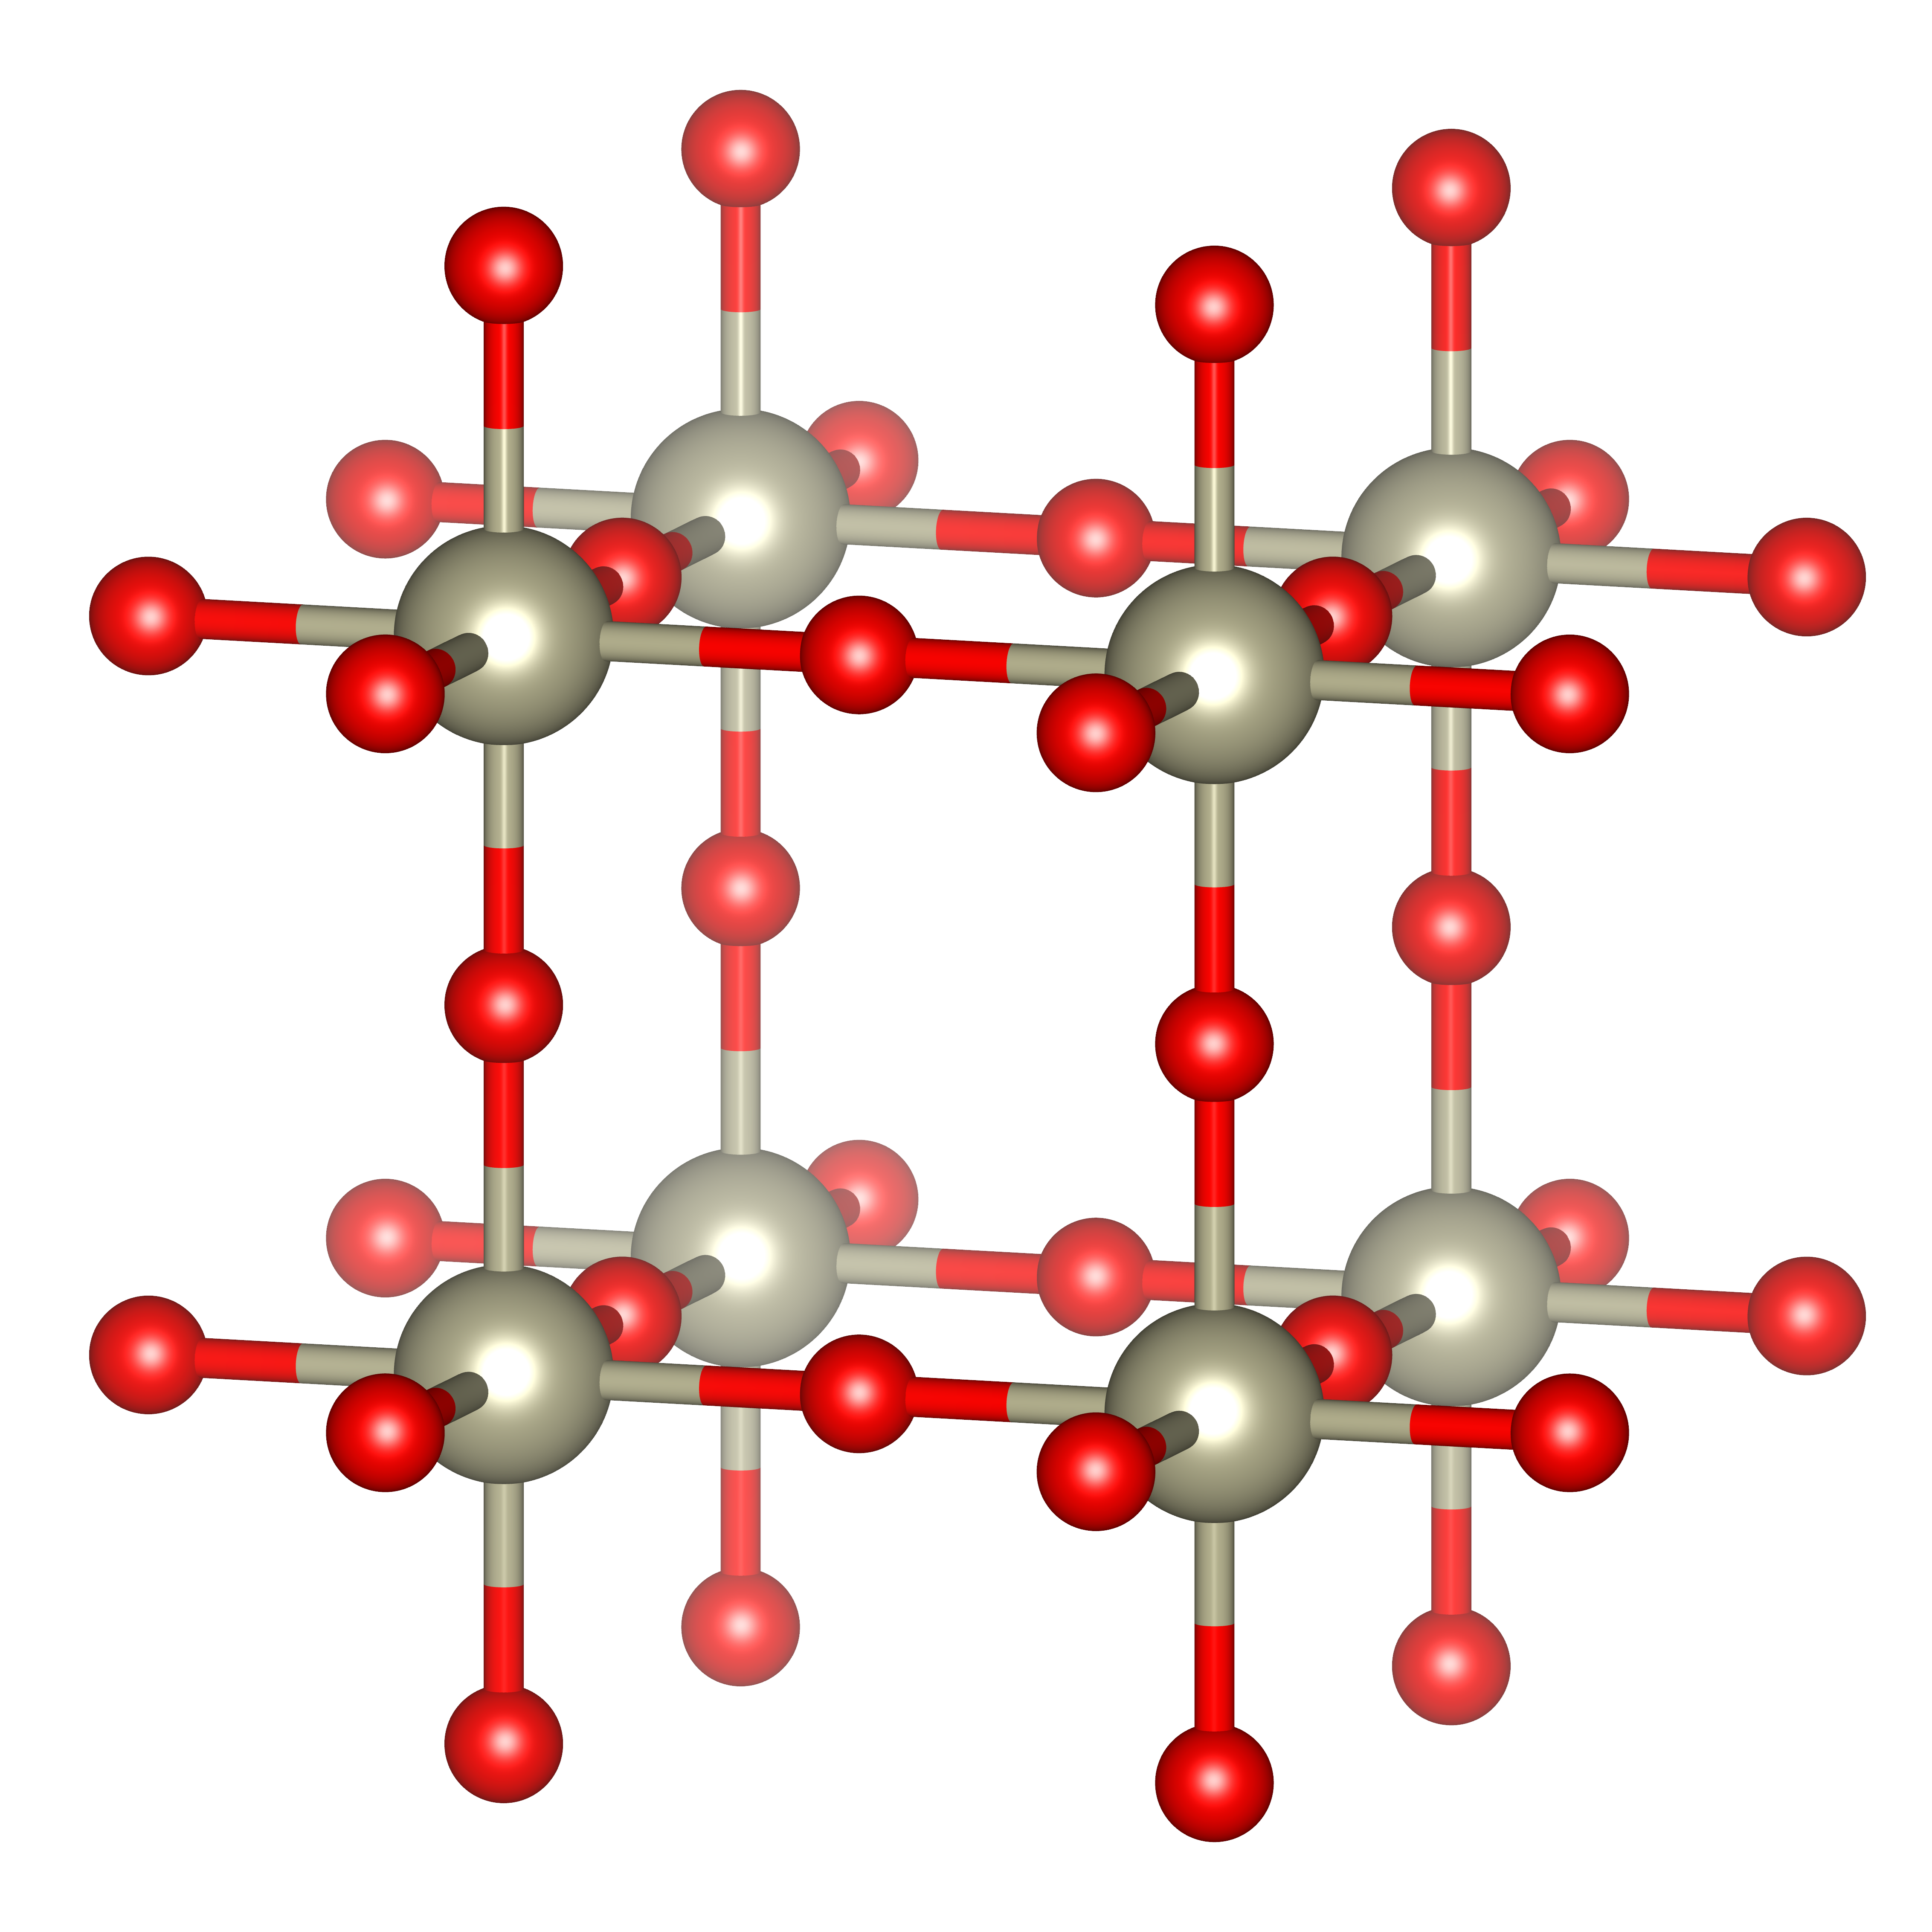
\includegraphics[scale=0.04]{Ch10/Halite/ReO3}
	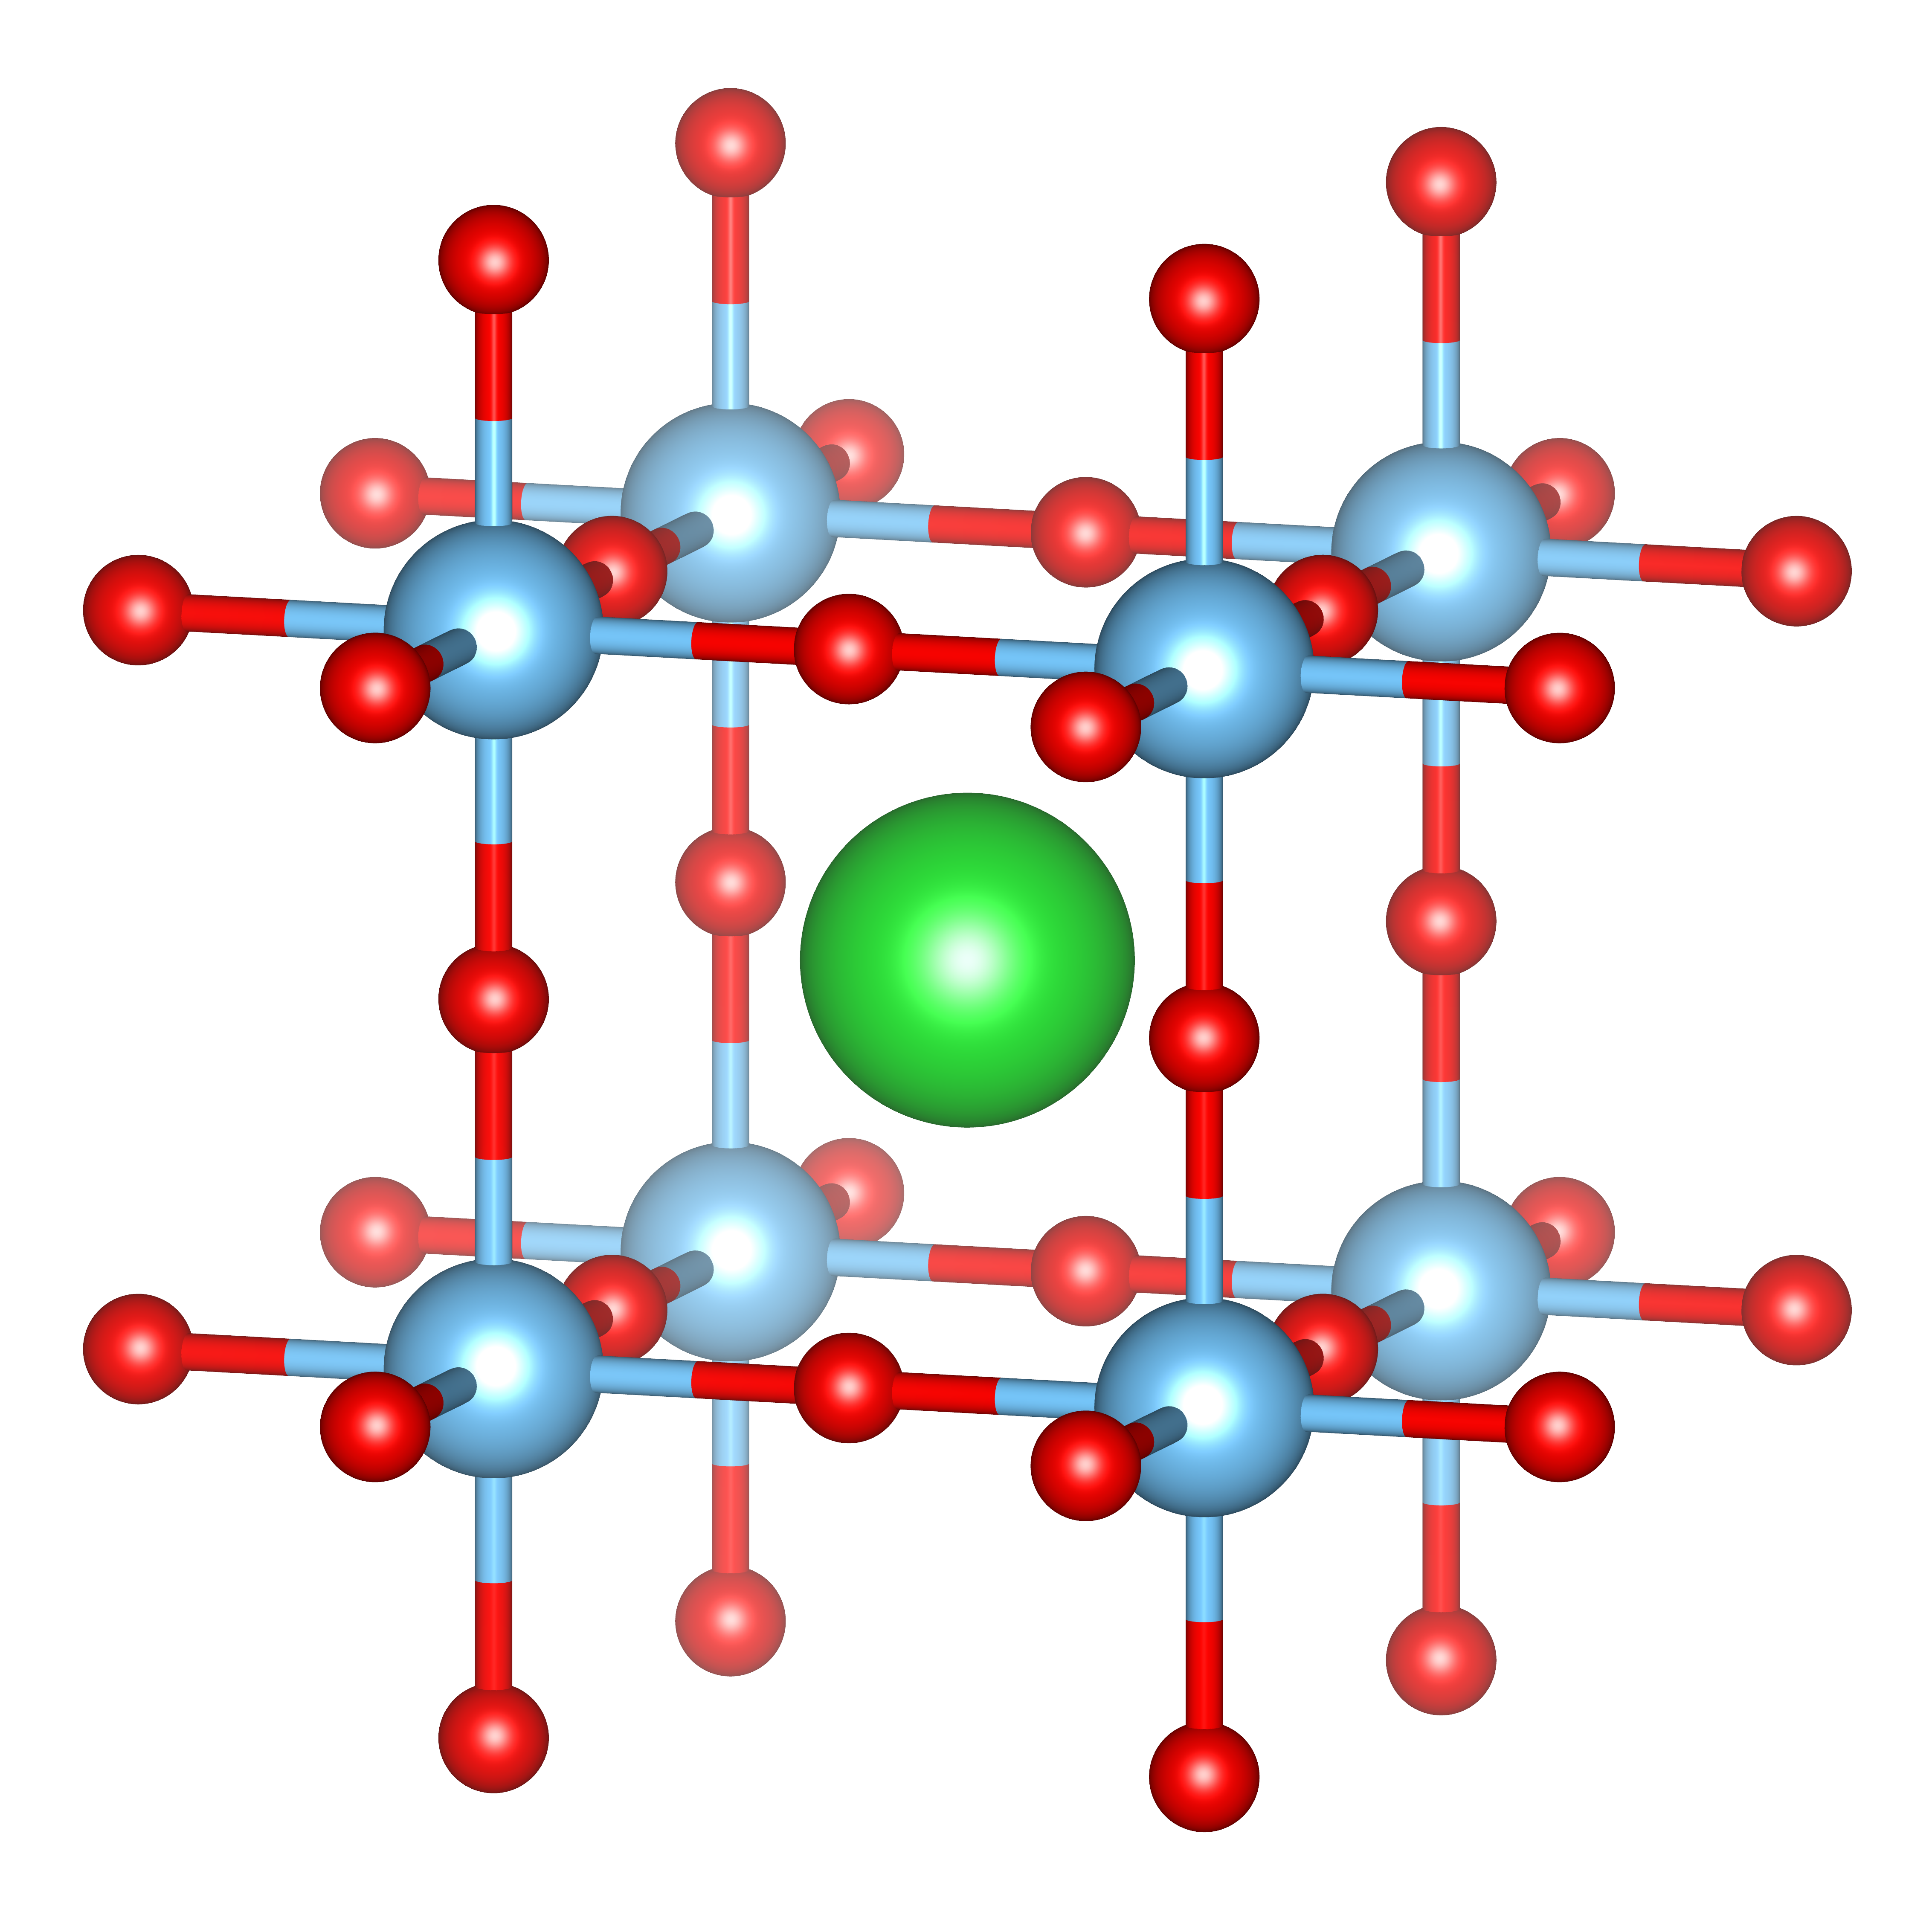
\includegraphics[scale=0.04]{Ch10/Perovskite/BaTiO3}
	\caption{$\rm NbO$, $\rm ReO_3$ and perovskite structure}
	\label{ReO3}
\end{figure}\ \\
%
The structure of tungsten trioxide $\rm WO_3$ is the same as $\rm ReO_3$. 
However, $\rm WO_3$ can be easily reduced. When it is reduced to $\rm NaWO_3$, 
the sodium atom will add to its body center, creating a new kind of structure called perovskites.\\ \\
Perovskites have a common formula $\rm ABX_3$, where: 
%
\begin{itemize}
	\item A is usually a soft large cation as lanthanides or late alkali (earth) metals;
	\item B is usually a hard small cation as in the case of high-valent transition metals;
	\item X can be oxygen or halogens, most commonly seen oxygen and iodine.
\end{itemize}
%
The structure of perovskites can be described as: A and X stack together into closest-packing at ratio 1:3, 
and B atoms fill in all the octahedral site whose vertices are all X. 
If A and X packs into ccp, then a cubic cell can be assigned.
In a cubic cell the $\rm [BX_6]$ octahedra are connected with shared vertices
and stack in three axial directions.
Figure \ref{batio3} presentes this process with $\bullet$ and $\circ$ showing two different layers, 
$\times$ refering to one B atom.\\
%
\begin{figure}[h]
	\centering
	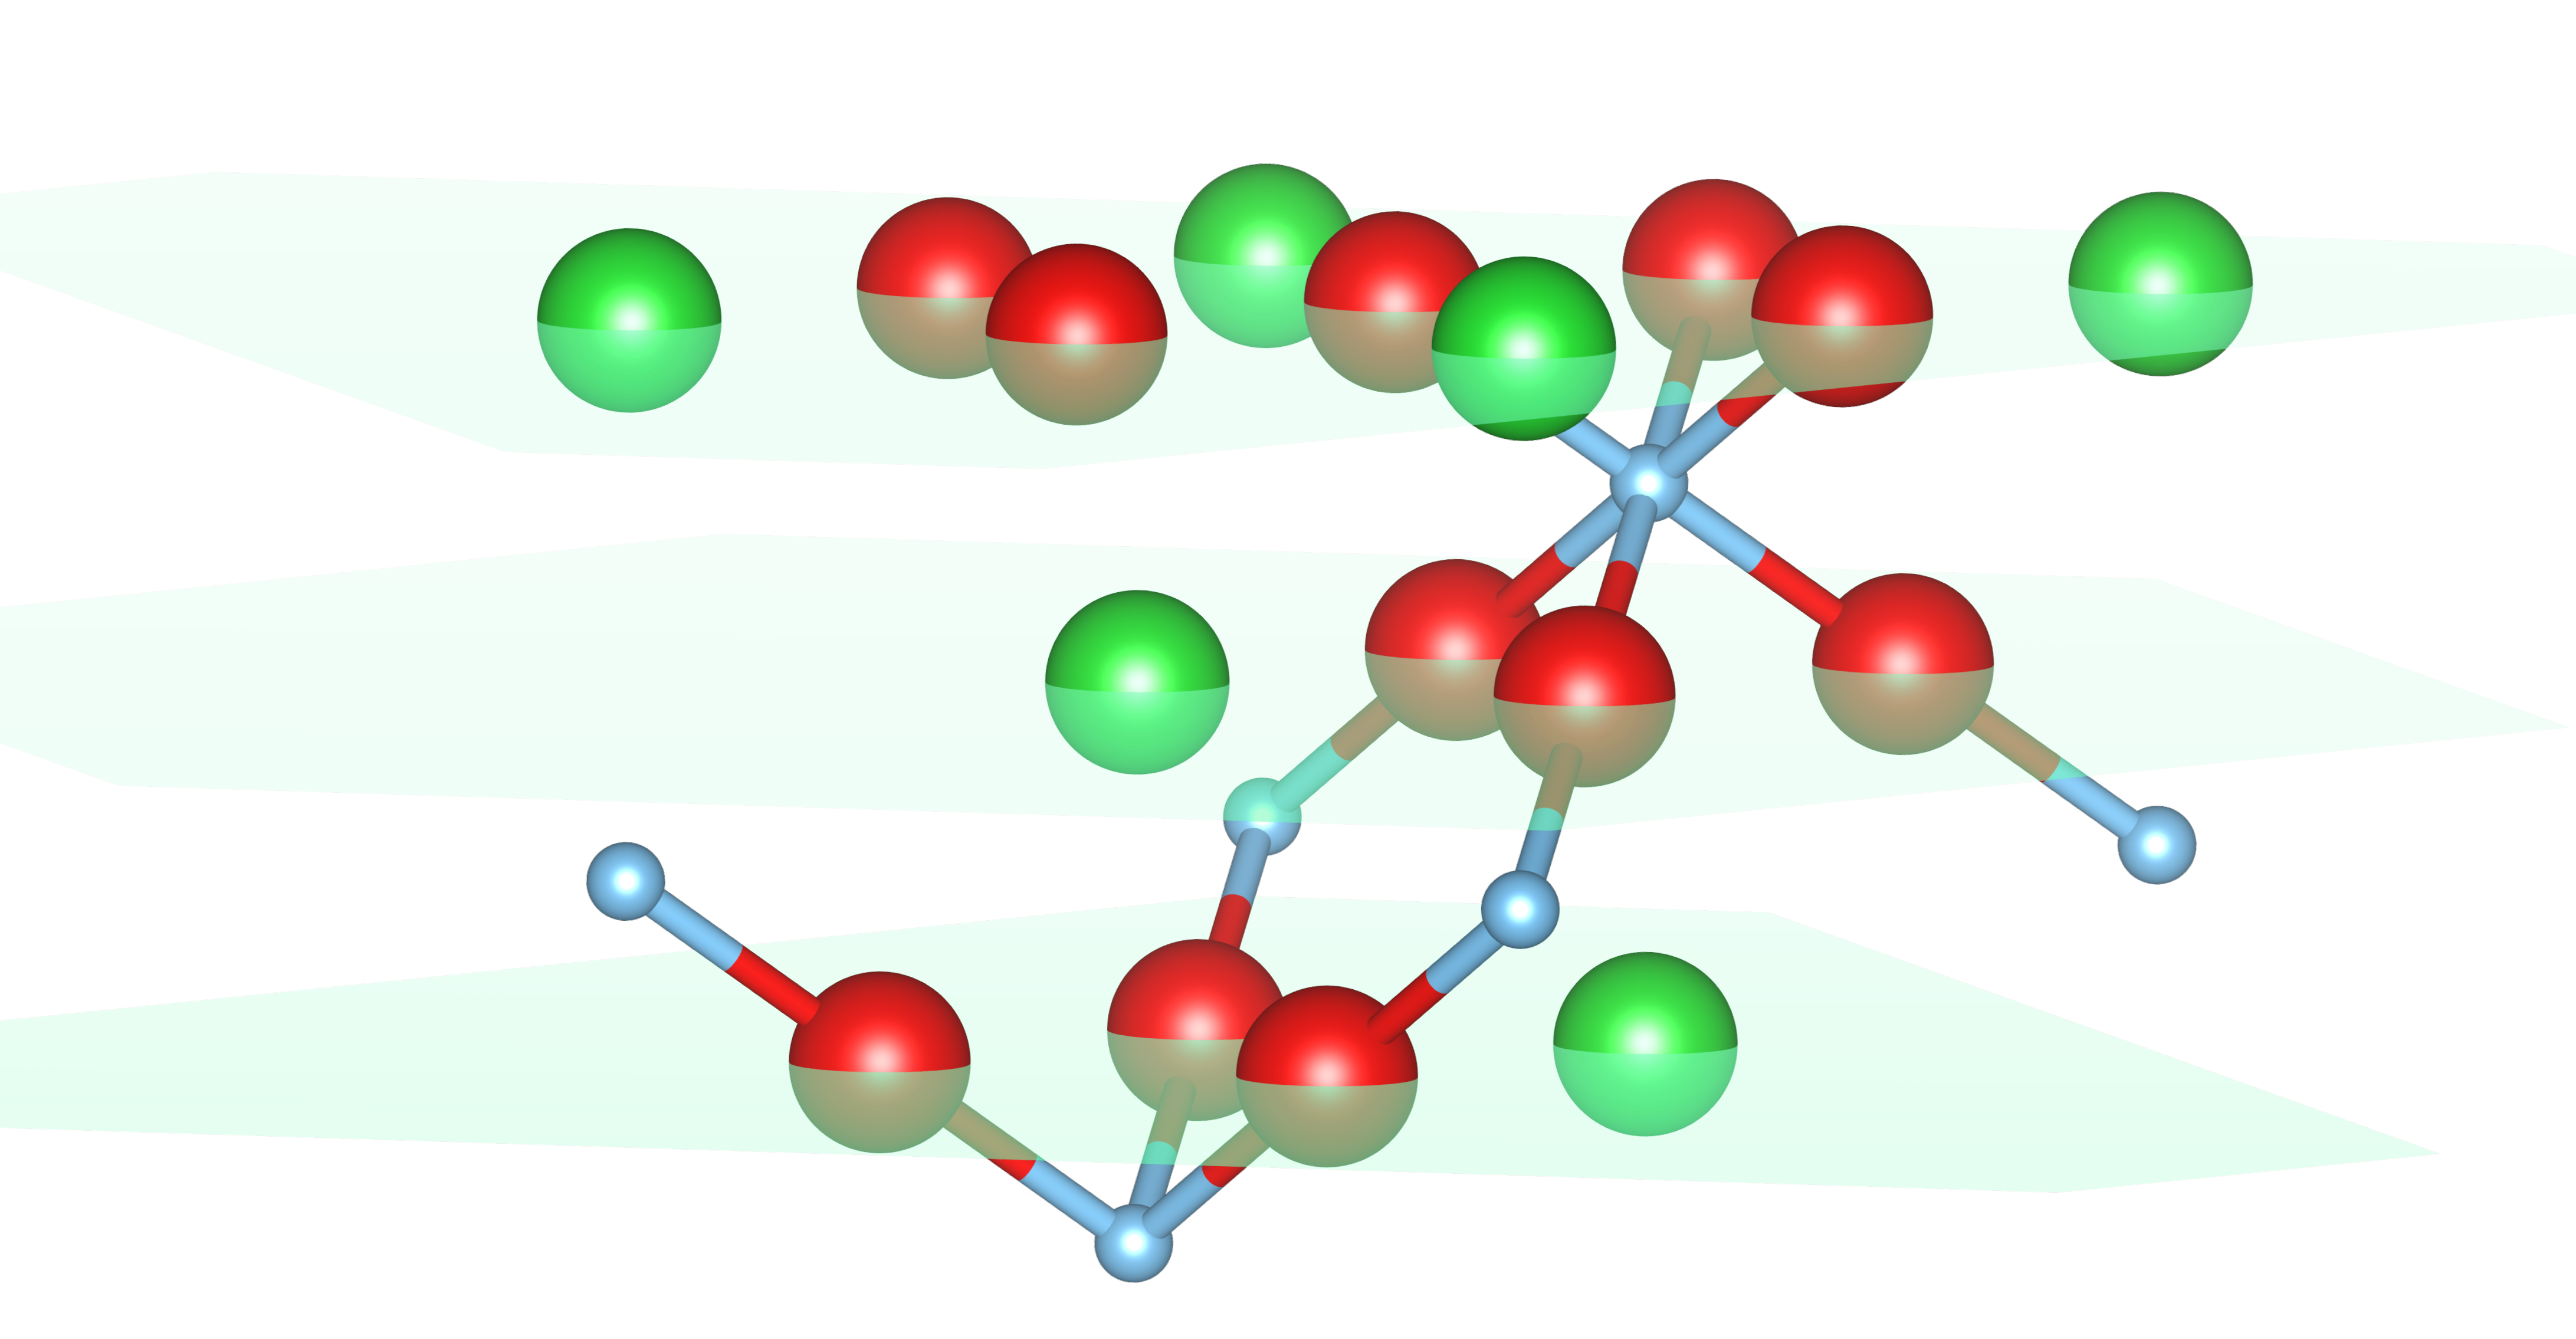
\includegraphics[scale=0.06]{Ch10/Perovskite/BaTiO3_pack}
	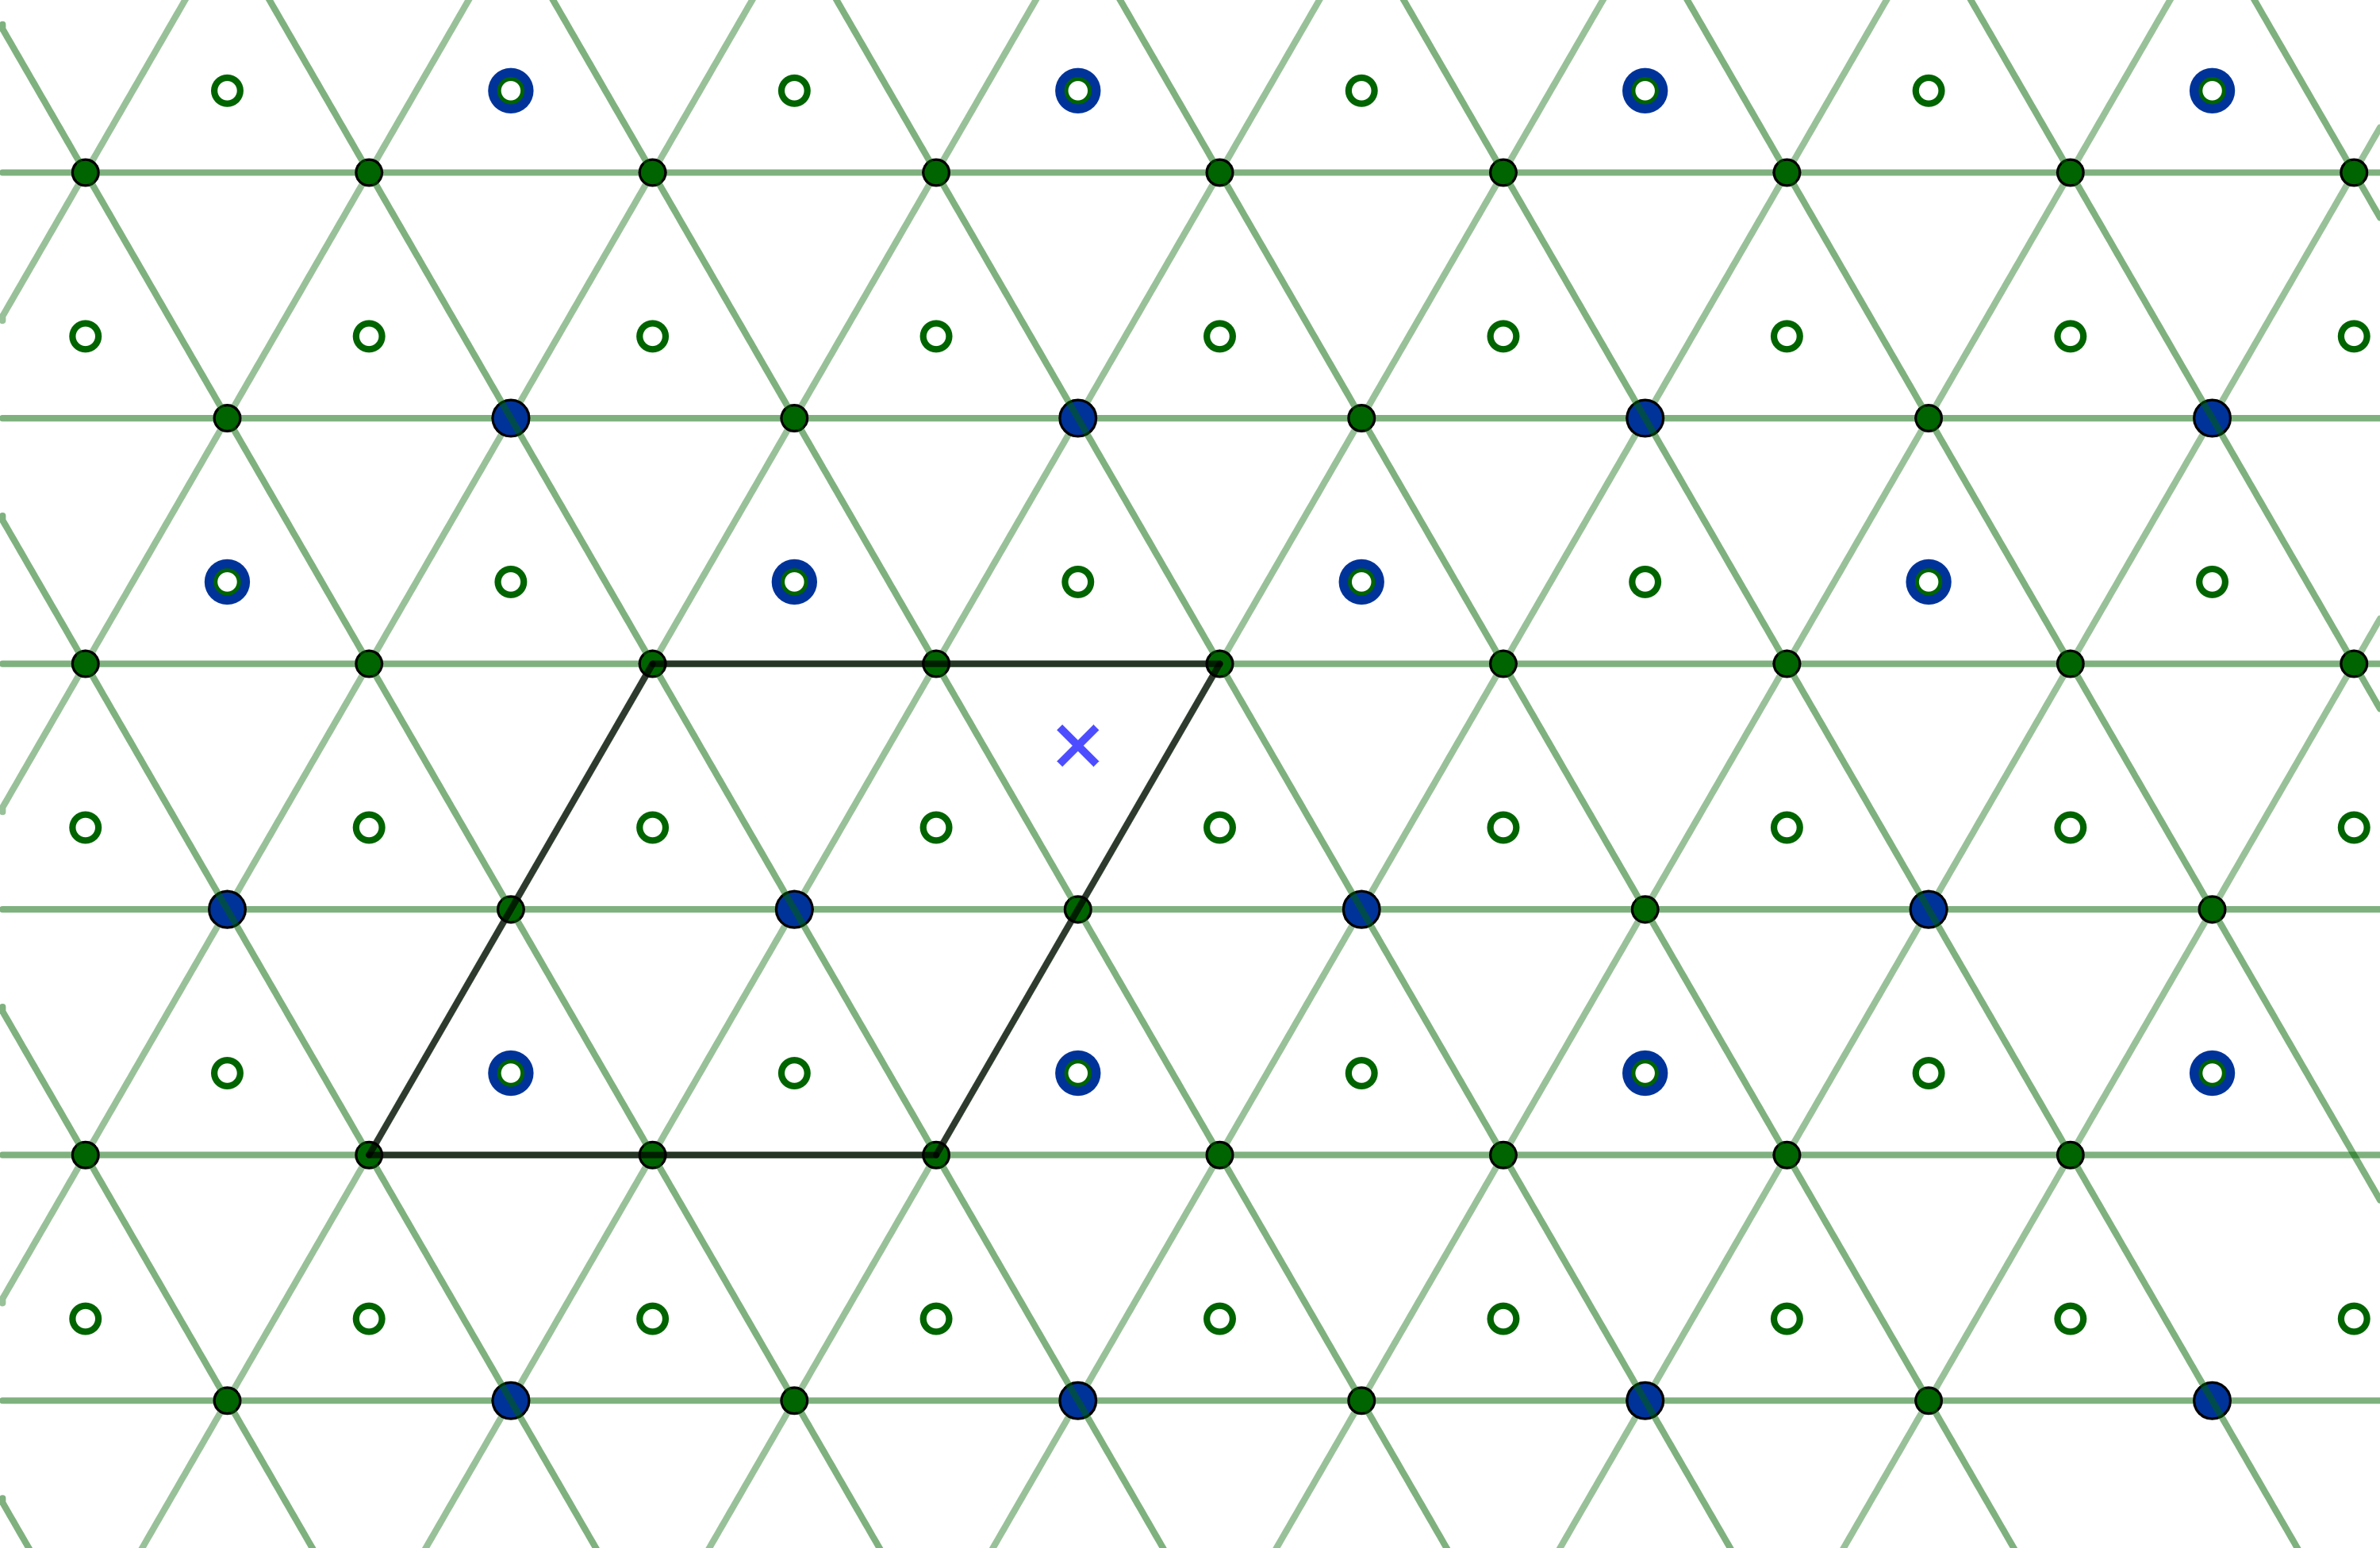
\includegraphics[scale=0.56]{Ch10/Perovskite/BaTiO3_layer}
	\caption{The closest-packing layers of cubic perovskite}
	\label{batio3}
\end{figure}\ \\
%
In the cubic cell if all atoms are tangent spheres, the following equation should hold:
%
\[
	r_A + r_X = \sqrt{2}(r_B + r_X)
\]
%
However in real cases some small distortion is allowed. We define Goldshmidt's tolerance factor:
%
\[
	t = \frac{r_A + r_X}{\sqrt{2}(r_B + r_X)} \in [0.7,1.0]
\]
%
If A is too small compared to its truncated cubic coordination, i.e. factor $t$ too small, 
the $\rm [BX_6]$ octahedrons will rotate inwards to shrink the volume of the truncated cube. 
Consequently the symmetry will be downgraded to tetragonal (if the rotation occurred in the plane, as in $\rm CsSnI_3$) or 
orthogonal (as in $\rm LaCrO_3$). The distortion into tetragonal lattice is shown in figure \ref{distort1}.\\
%
\begin{figure}[h]
	\centering
	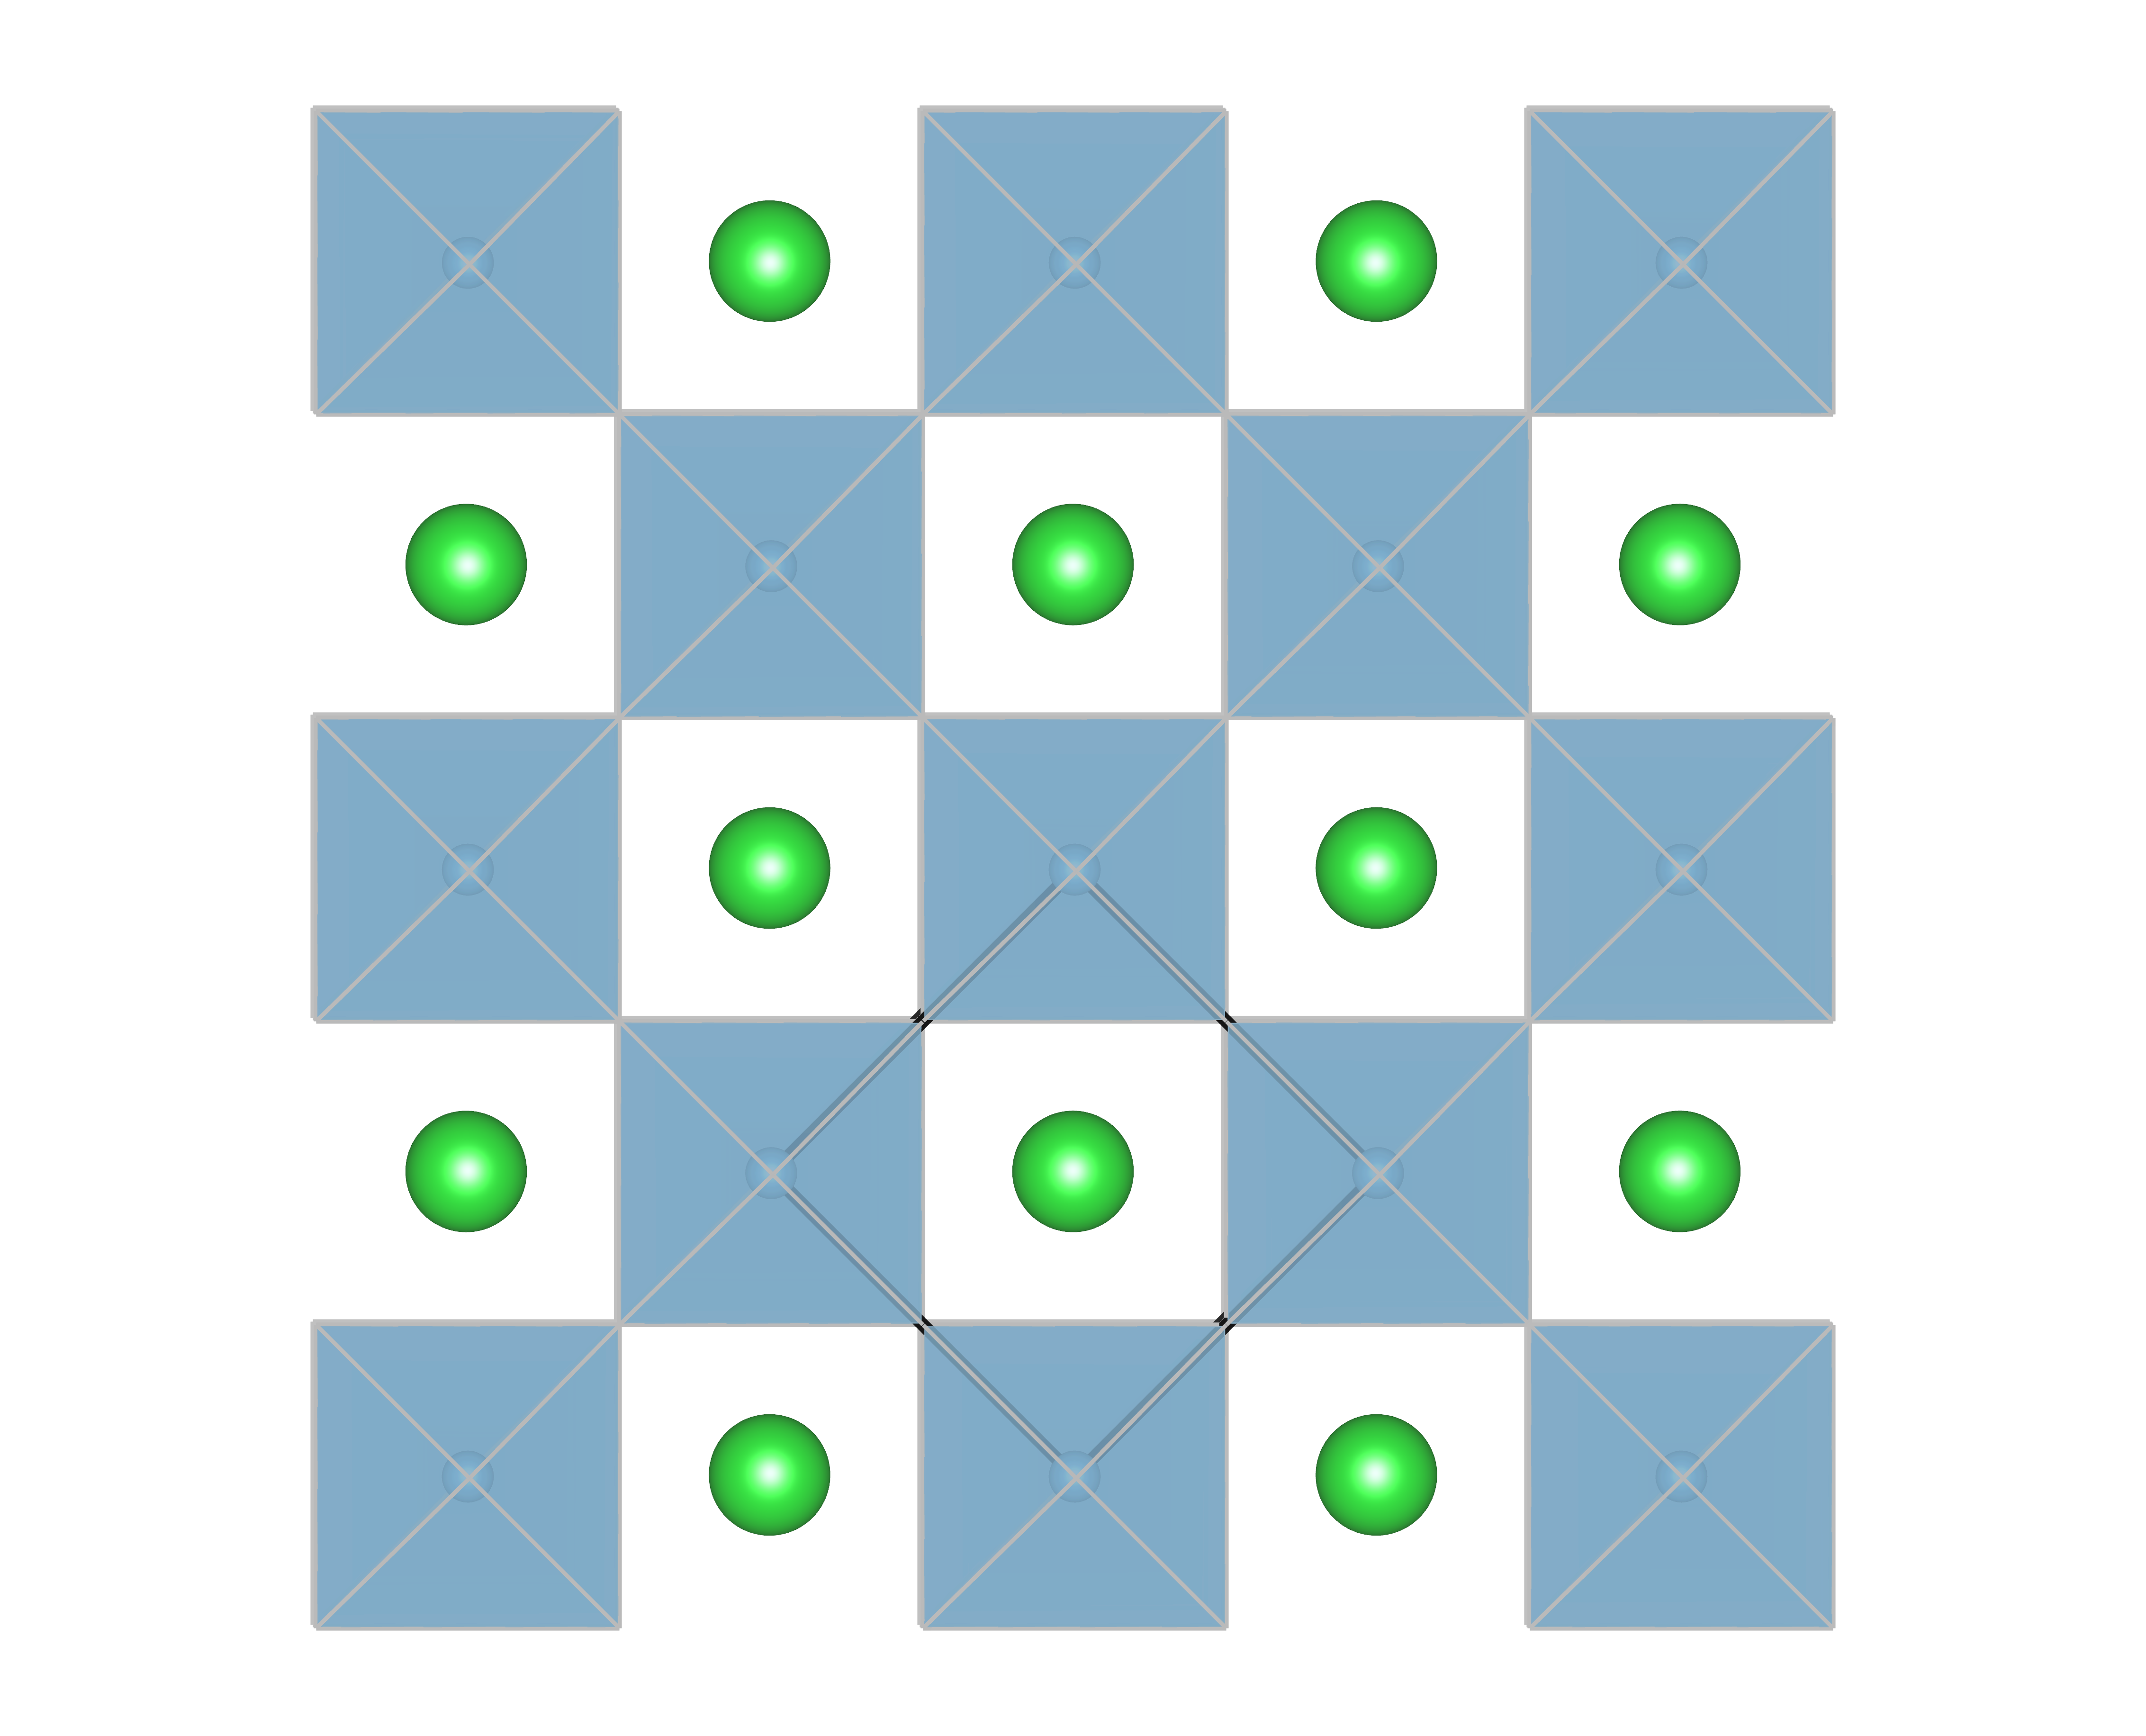
\includegraphics[scale=0.04]{Ch10/Perovskite/BaTiO3_distort}
	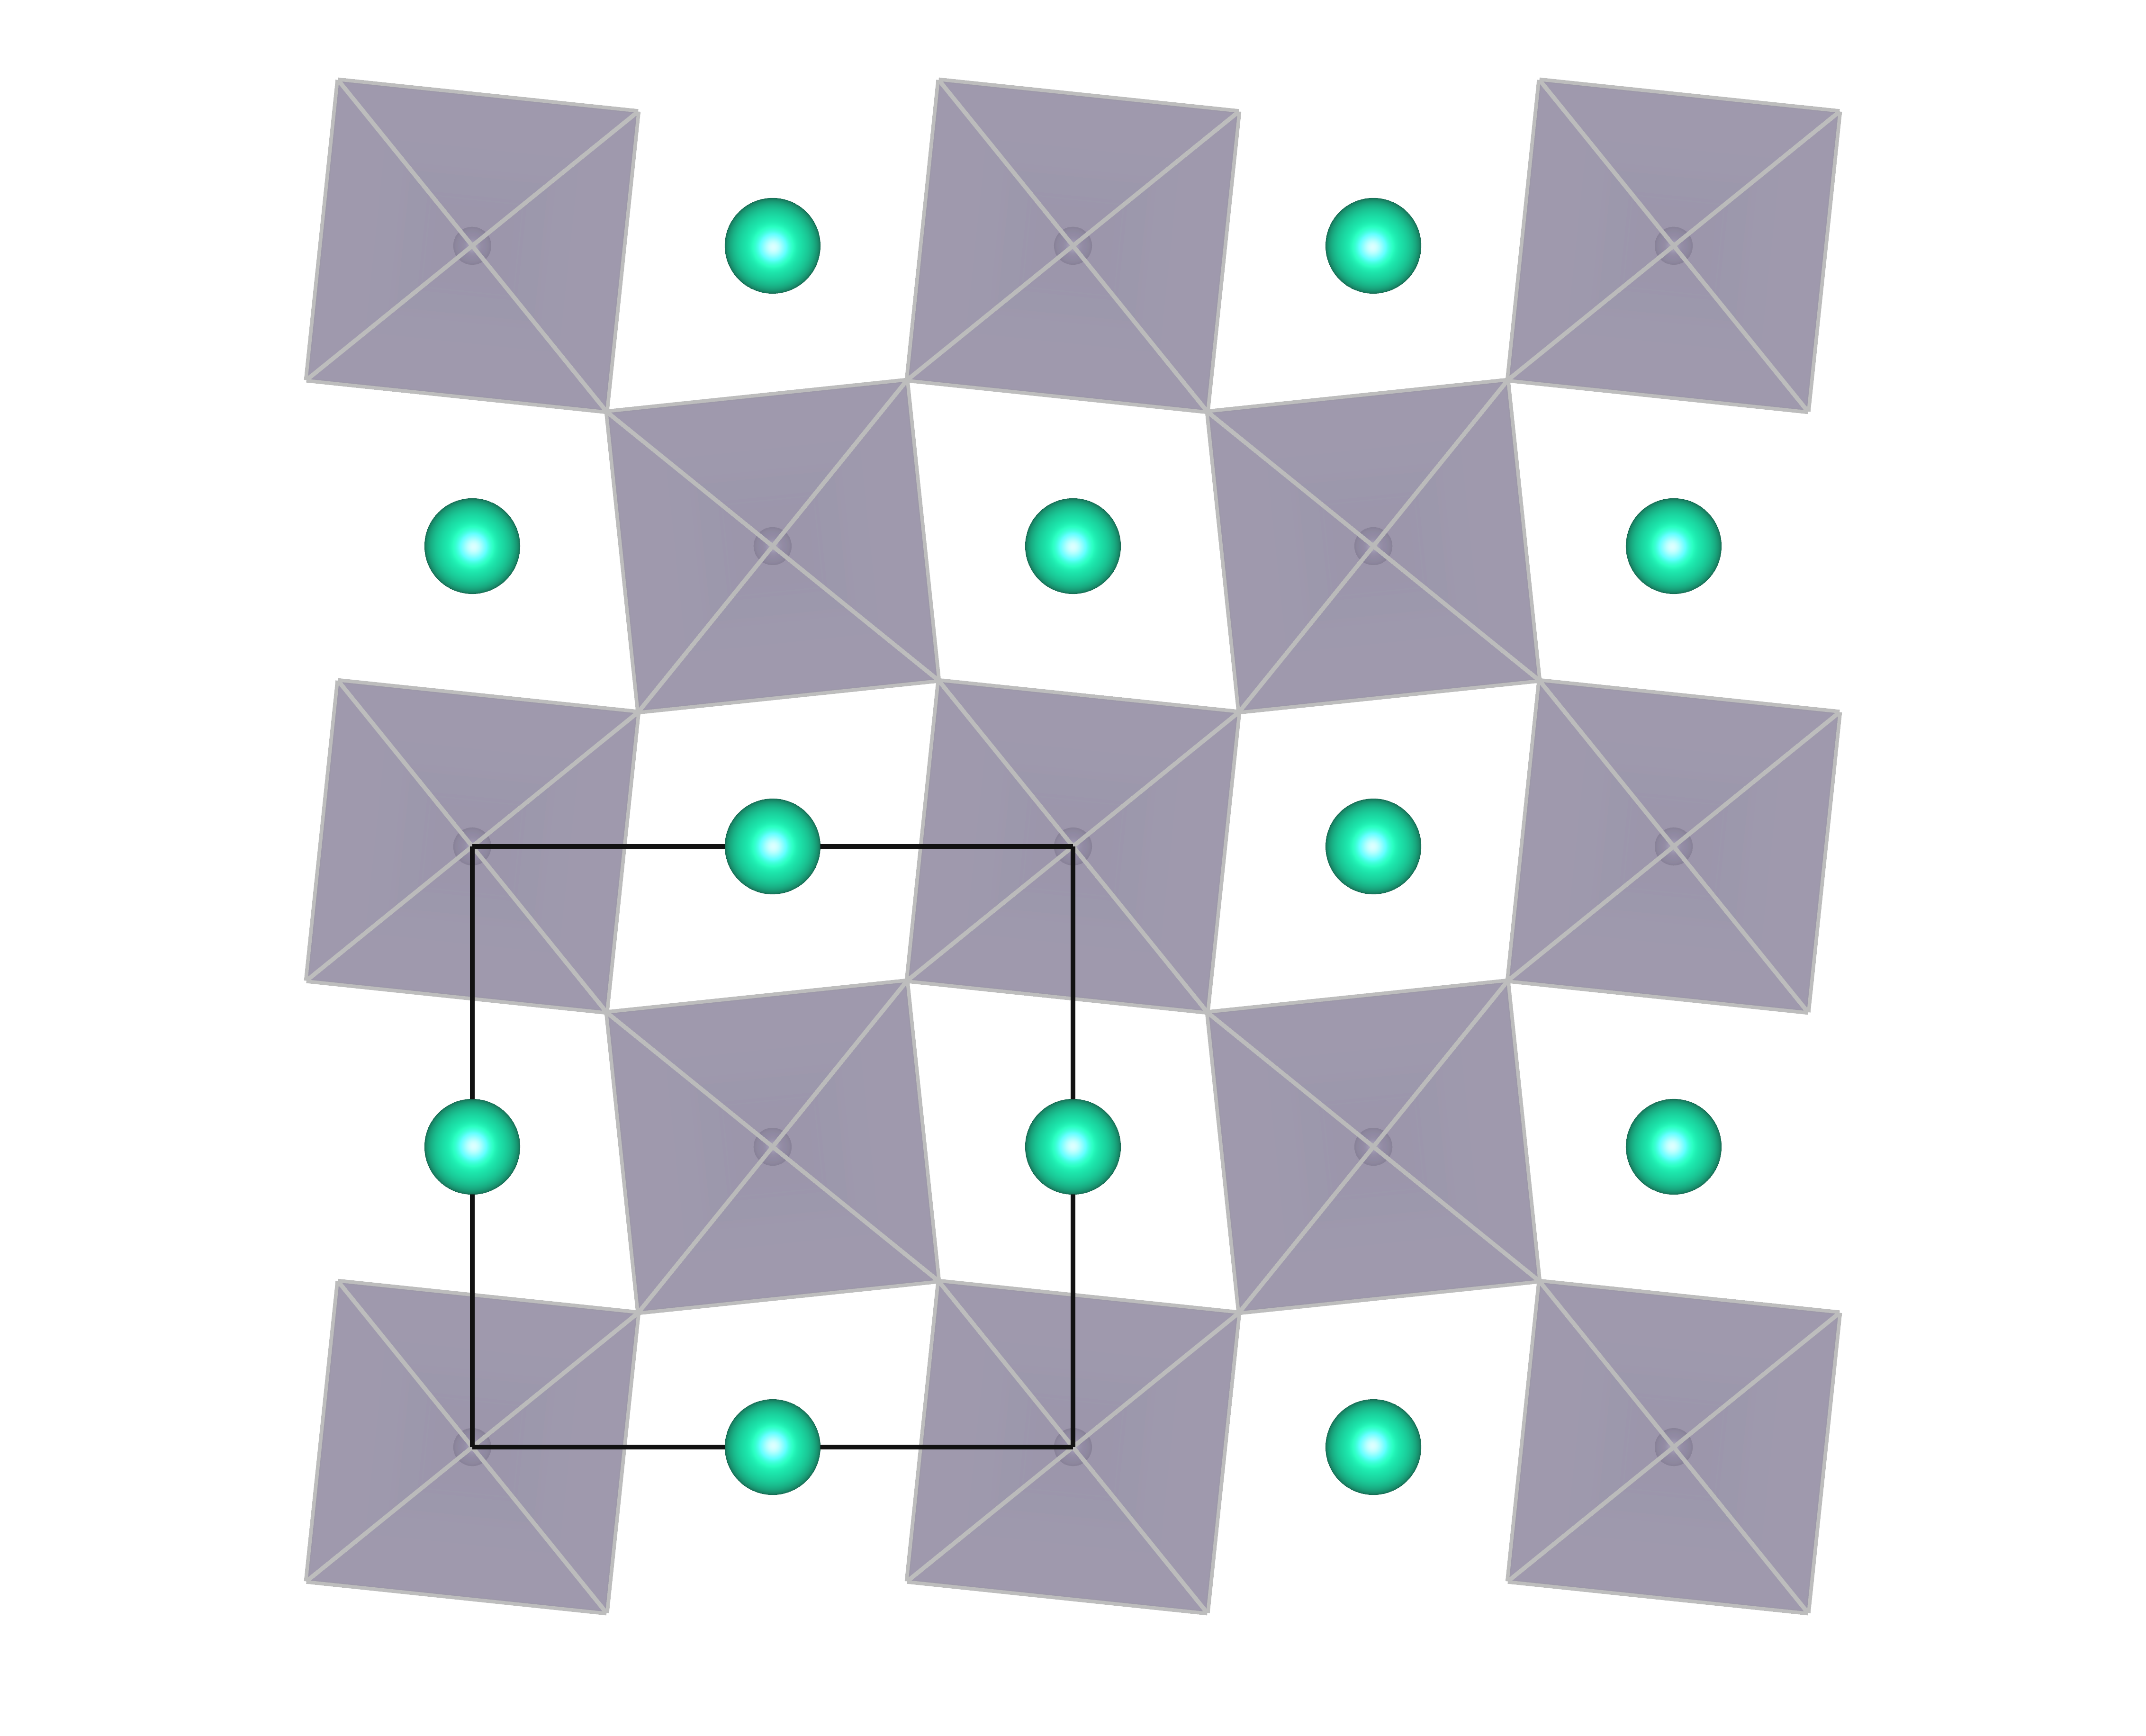
\includegraphics[scale=0.04]{Ch10/Perovskite/CsSnI3}
	\caption{Distortion of perovskite structure, $\rm BaTiO_3$ $(cP)$ and $\rm CsSnI_3$ $(tP)$.}
	\label{distort1}
\end{figure}\ \\
%
By contrast, if B is too small for its octahedron, i.e. factor $t$ too large,
every B atom will undergo off-center displacement to ensure its bonding to some of the six X atoms rather than weaken all six bonds,
downgrading the symmetry to tetragonal or orthogonal, as shown in figure \ref{distort2}.
However, this creates a permanent electric dipole in the crystal, a property named ferroelectricity.\\
%
\begin{figure}[h]
	\centering
	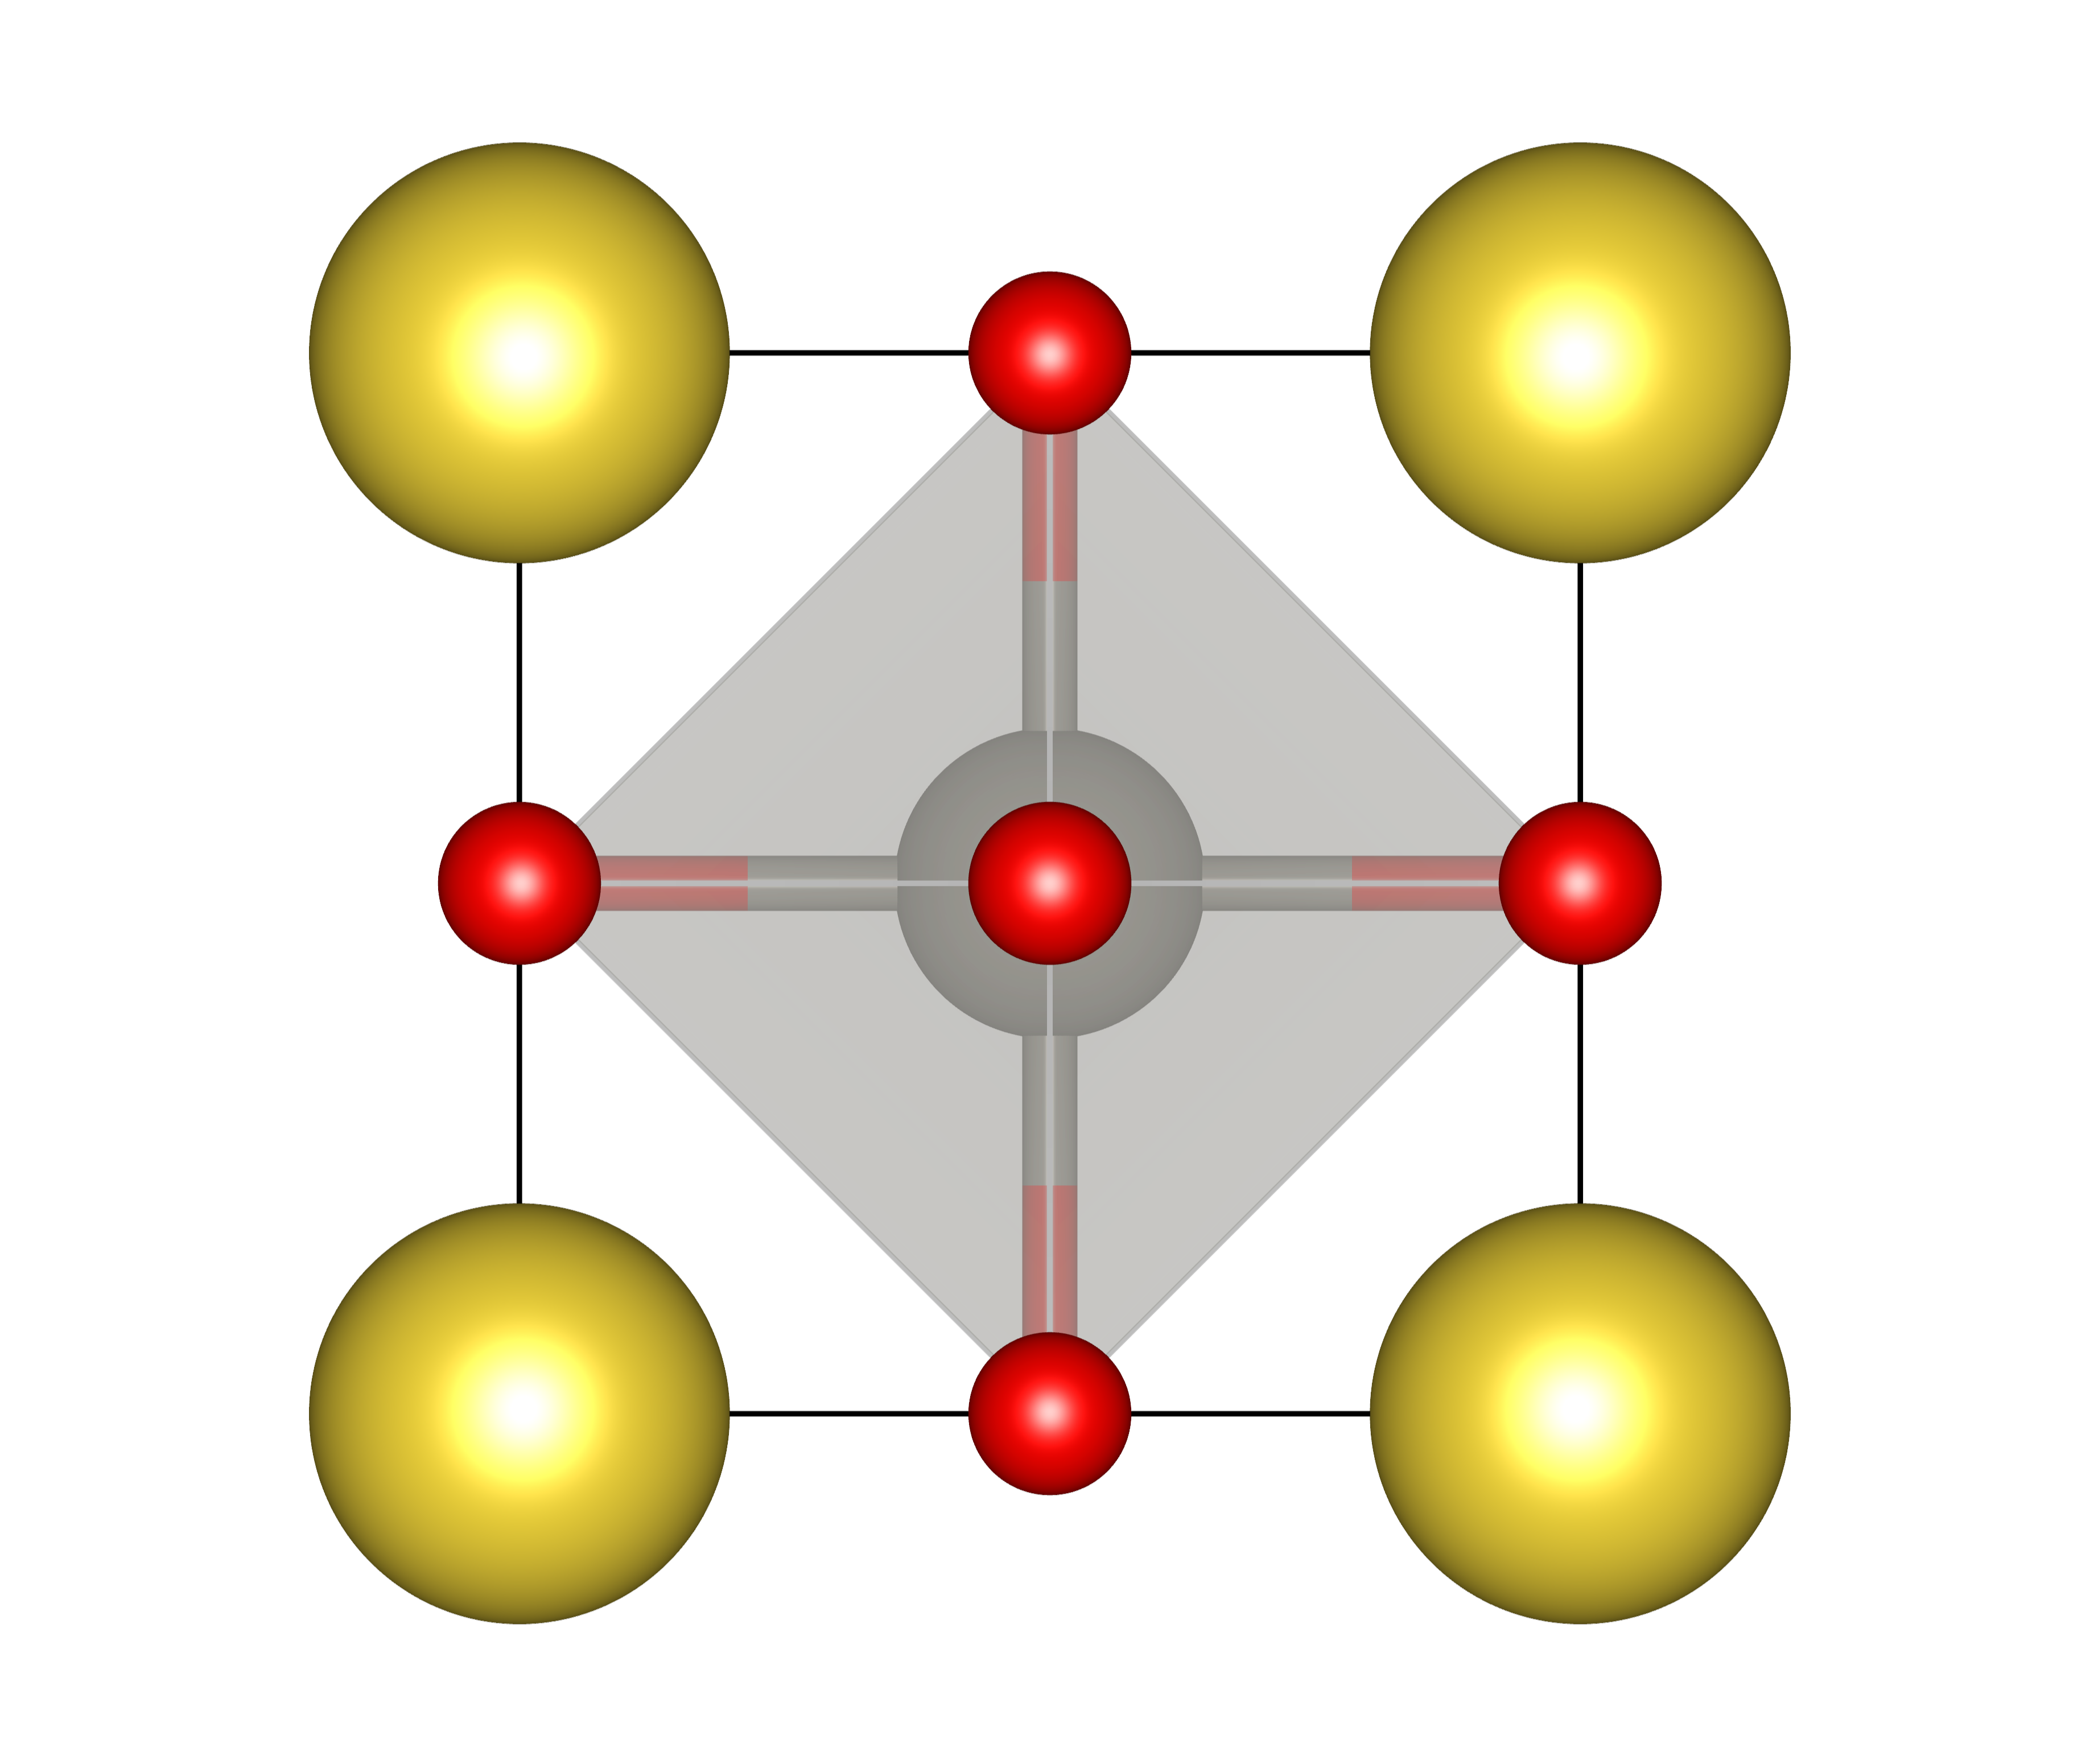
\includegraphics[scale=0.04]{Ch10/Perovskite/NaWO3}
	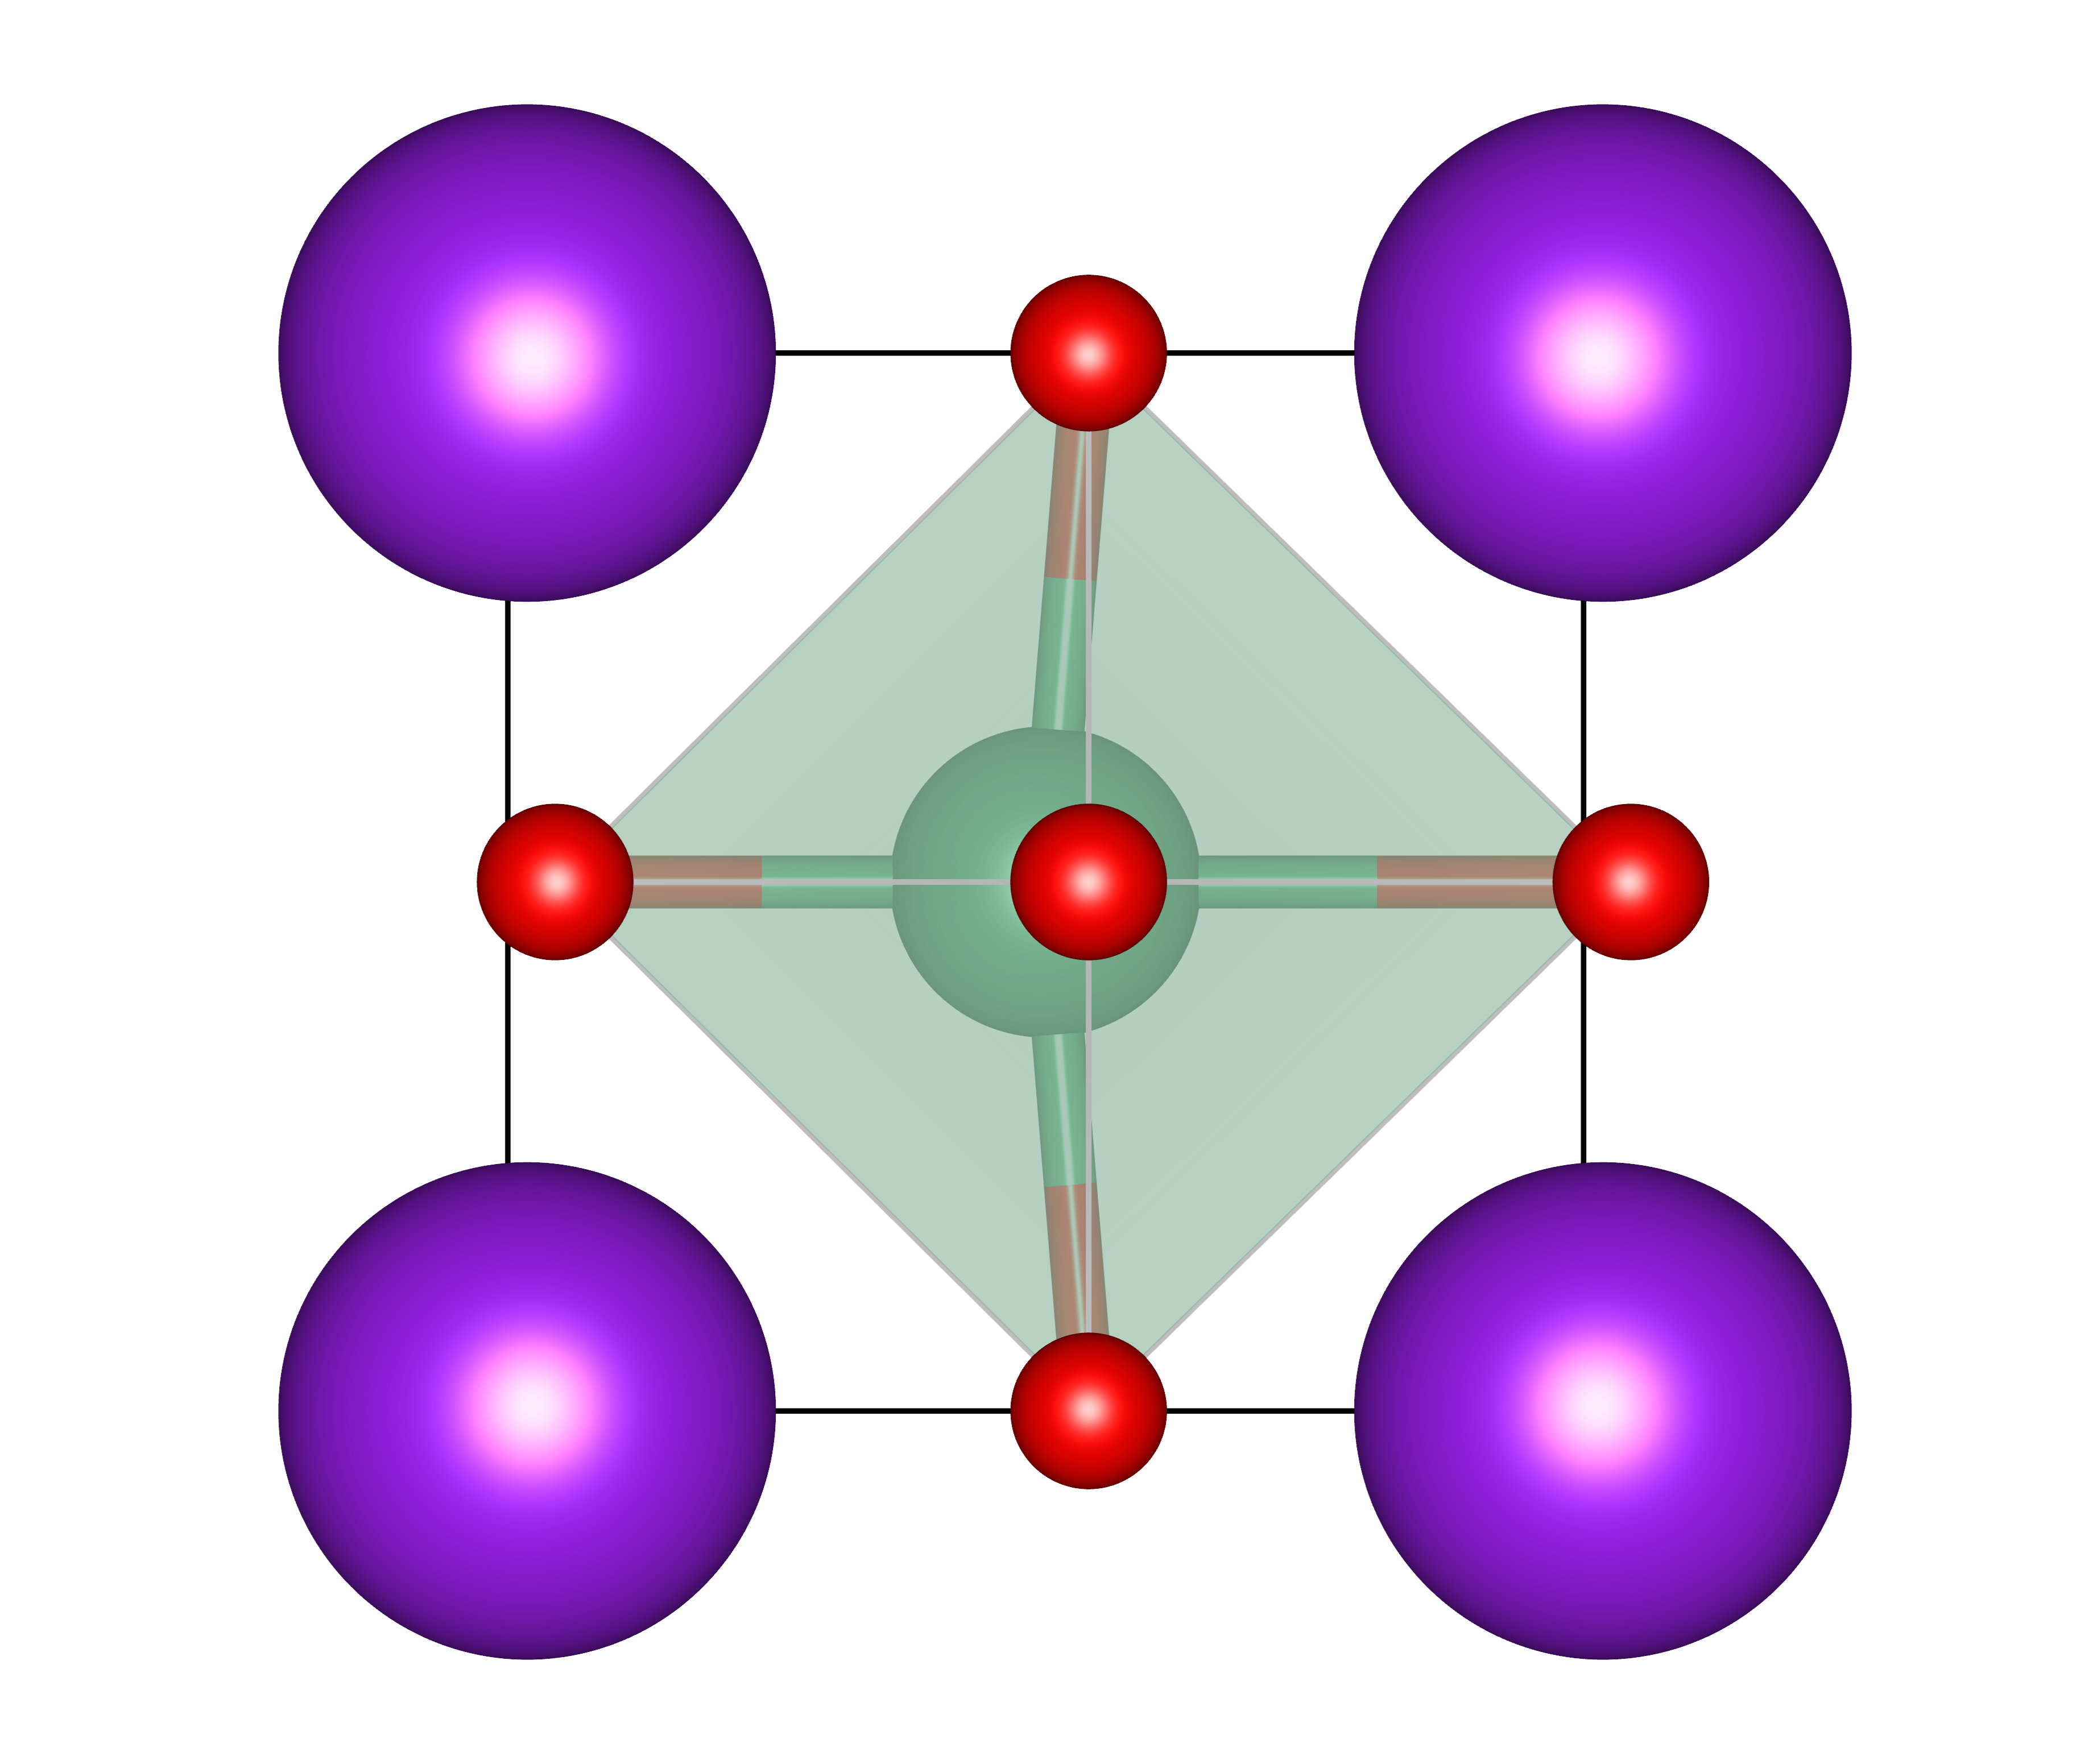
\includegraphics[scale=0.04]{Ch10/Perovskite/KNbO3}
	\caption{Off-center displacement of perovskite structure, $\rm NaWO_3$ $(cP)$ and $\rm KNbO_3$ $(tP)$.}
	\label{distort2}
\end{figure}\ \\
%
In addition, if $A$ is not just big but long, it may tear two layers of $\rm [BX_6]$ apart, 
changing the formula from $\rm ABX_3$ to $\rm A_2BX_4$, 
as in $\rm (^tBuNH_3)_2PbI_4$ where the heads of $\rm ^tBuNH_3$ is attracted to the $\rm [BX_6]$ due to Coulombic attraction, 
and van der Waals interaction holds their tails together. 
These structures, namely the 2D peroveskites, are illustrated in figure \ref{2dperov}.\\
%
%
\begin{figure}[h]
	\centering
	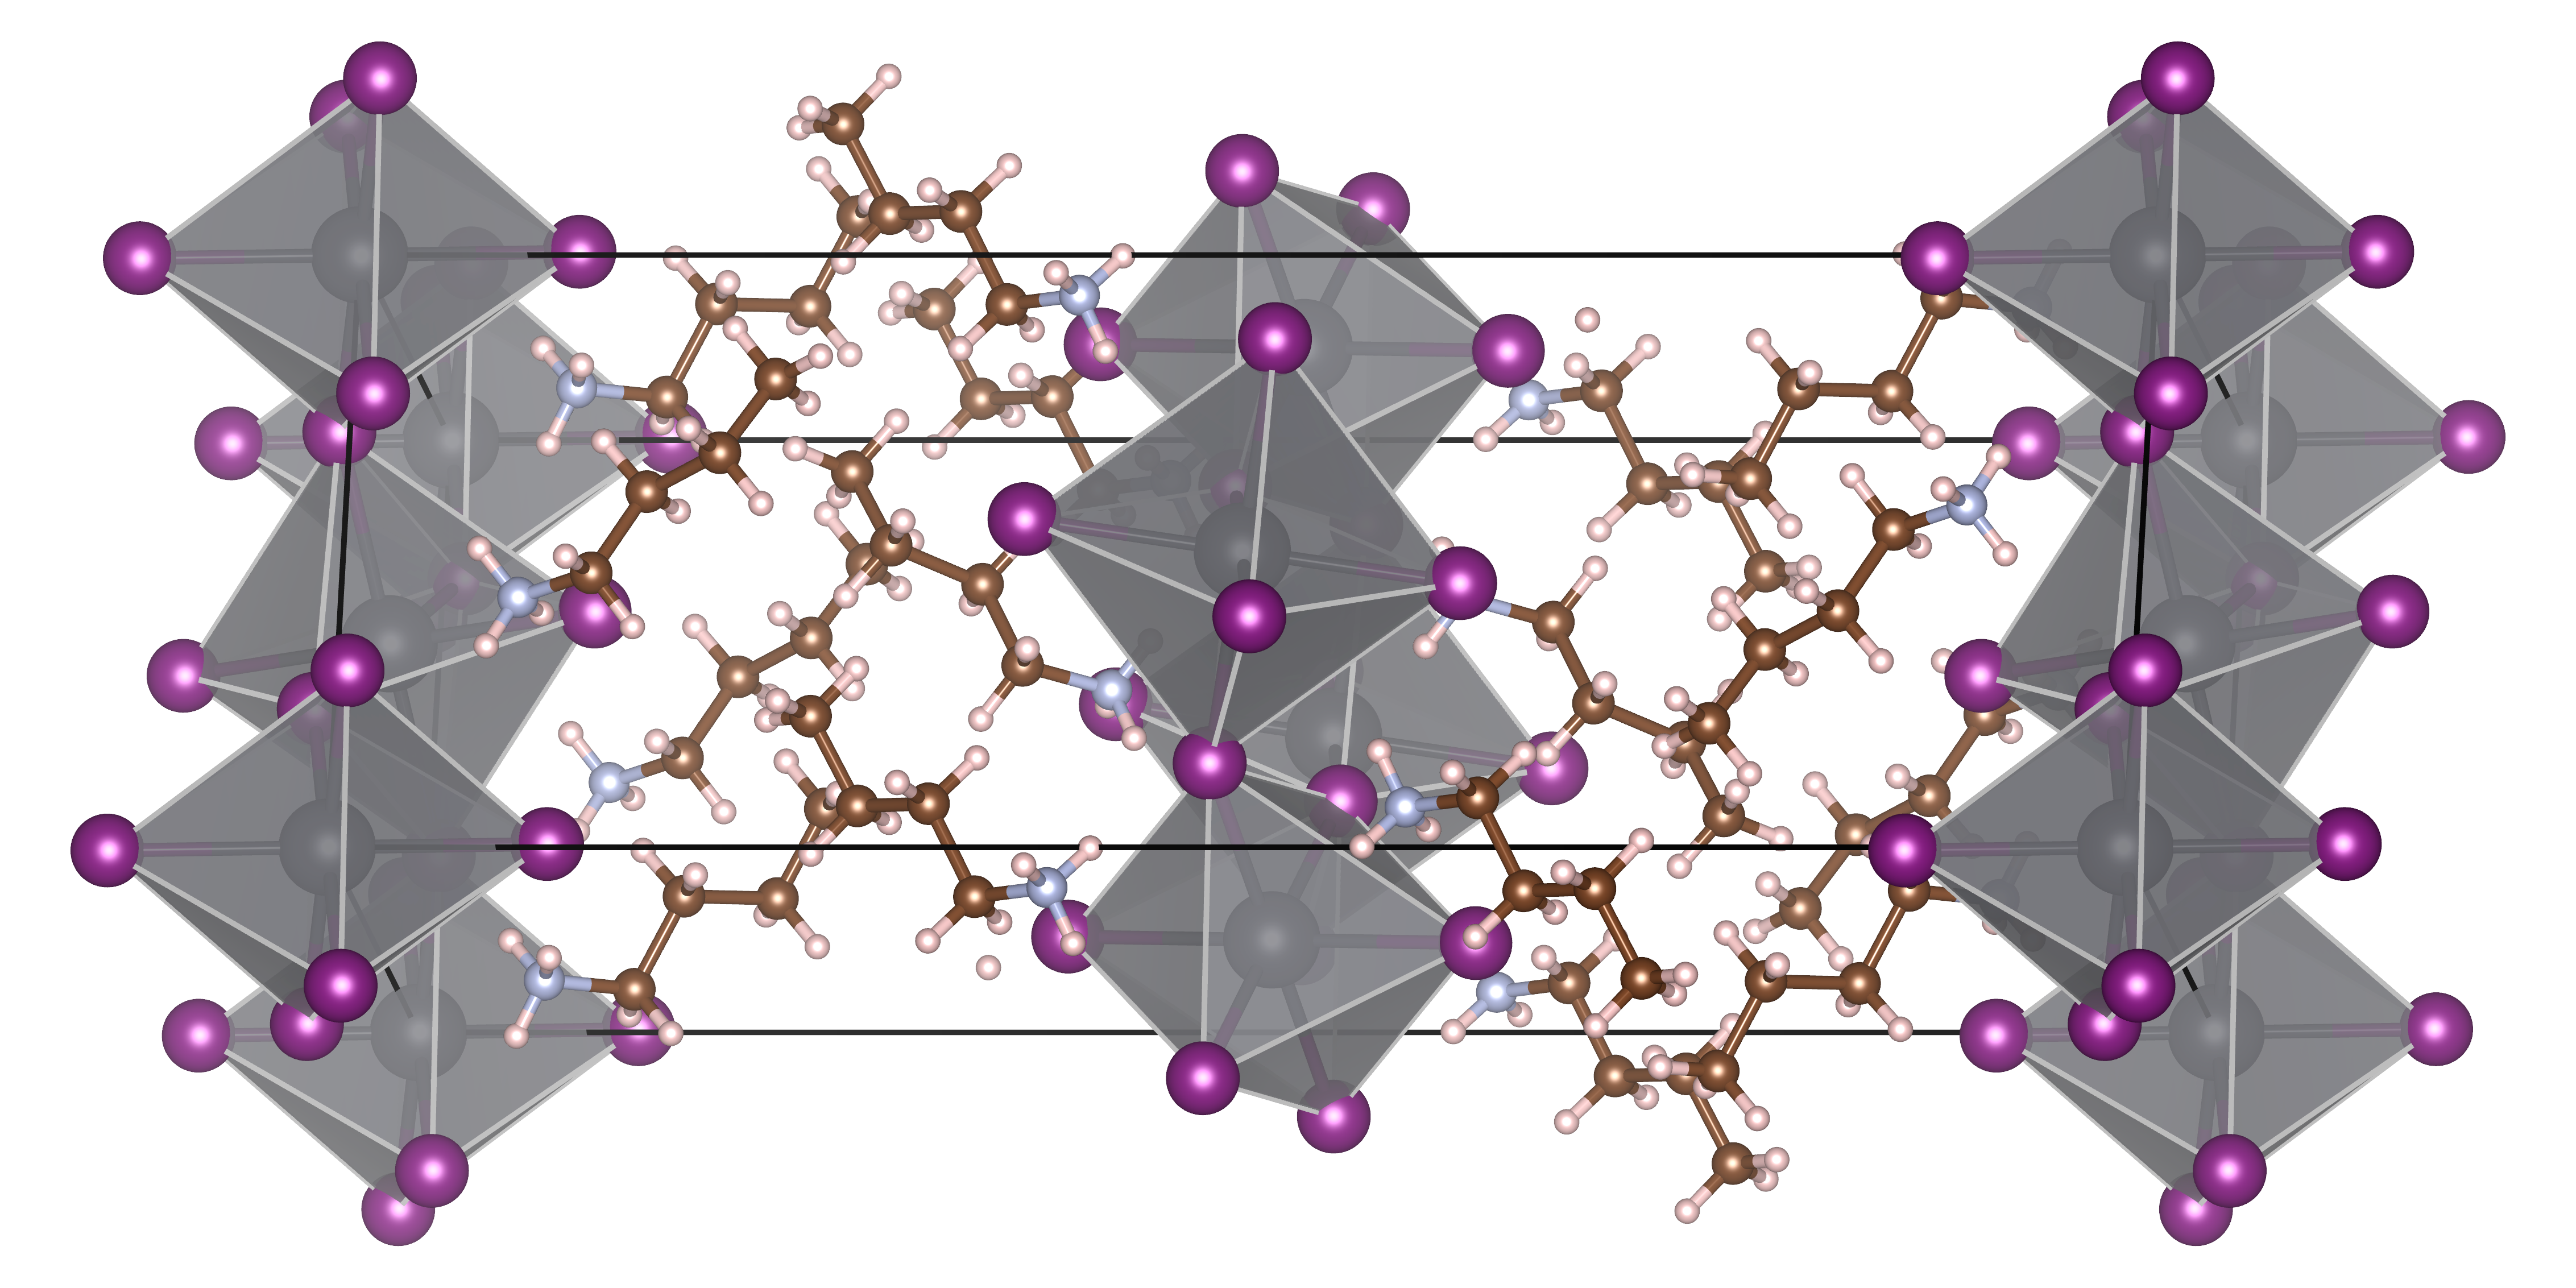
\includegraphics[scale=0.06]{Ch10/Perovskite/2dperovskite}
	\caption{Structure of 2D perovskites}
	\label{2dperov}
\end{figure}\ \\
%
Based on peroveskites and $\rm ReO_3$, if we replace spherical X with rod-shaped cyanides, we obtain the prussian blue/white structures
which is ready for redox reactions and accept +1 valent metal to enter its body center. 
Cyanides obey the HSAB principle with C-ends coordinate to softer lower-valent metals. 
Its vibrant color is brought by intermetallic charge transfer through cyanide bridges:
%
\[\rm
	(Electron\ rich)\underbrace{M \to C\equiv N \to M'}_
	{Cyanide\, polarize\, towards\, N,\, C\, accepts\, \pi\, backbonding}\ (Electron\, deficient)
\]
%
As $\rm CN^-$ is asymmetrical, its unit cell is 8 times larger than that of perovskites, as shown in figure \ref{fecn}.\\ \\
If we simply throw away the atoms on the edges, we are left with CsCl structure, as shown in figure \ref{cscl}. \label{cscls}
Note that ammonium chloride adopts this structure even if the radius of $\rm NH_4^+$ is comparable to that of $\rm K^+$ because of hydrogen bonds.
%
\begin{figure}[h]
	\centering
	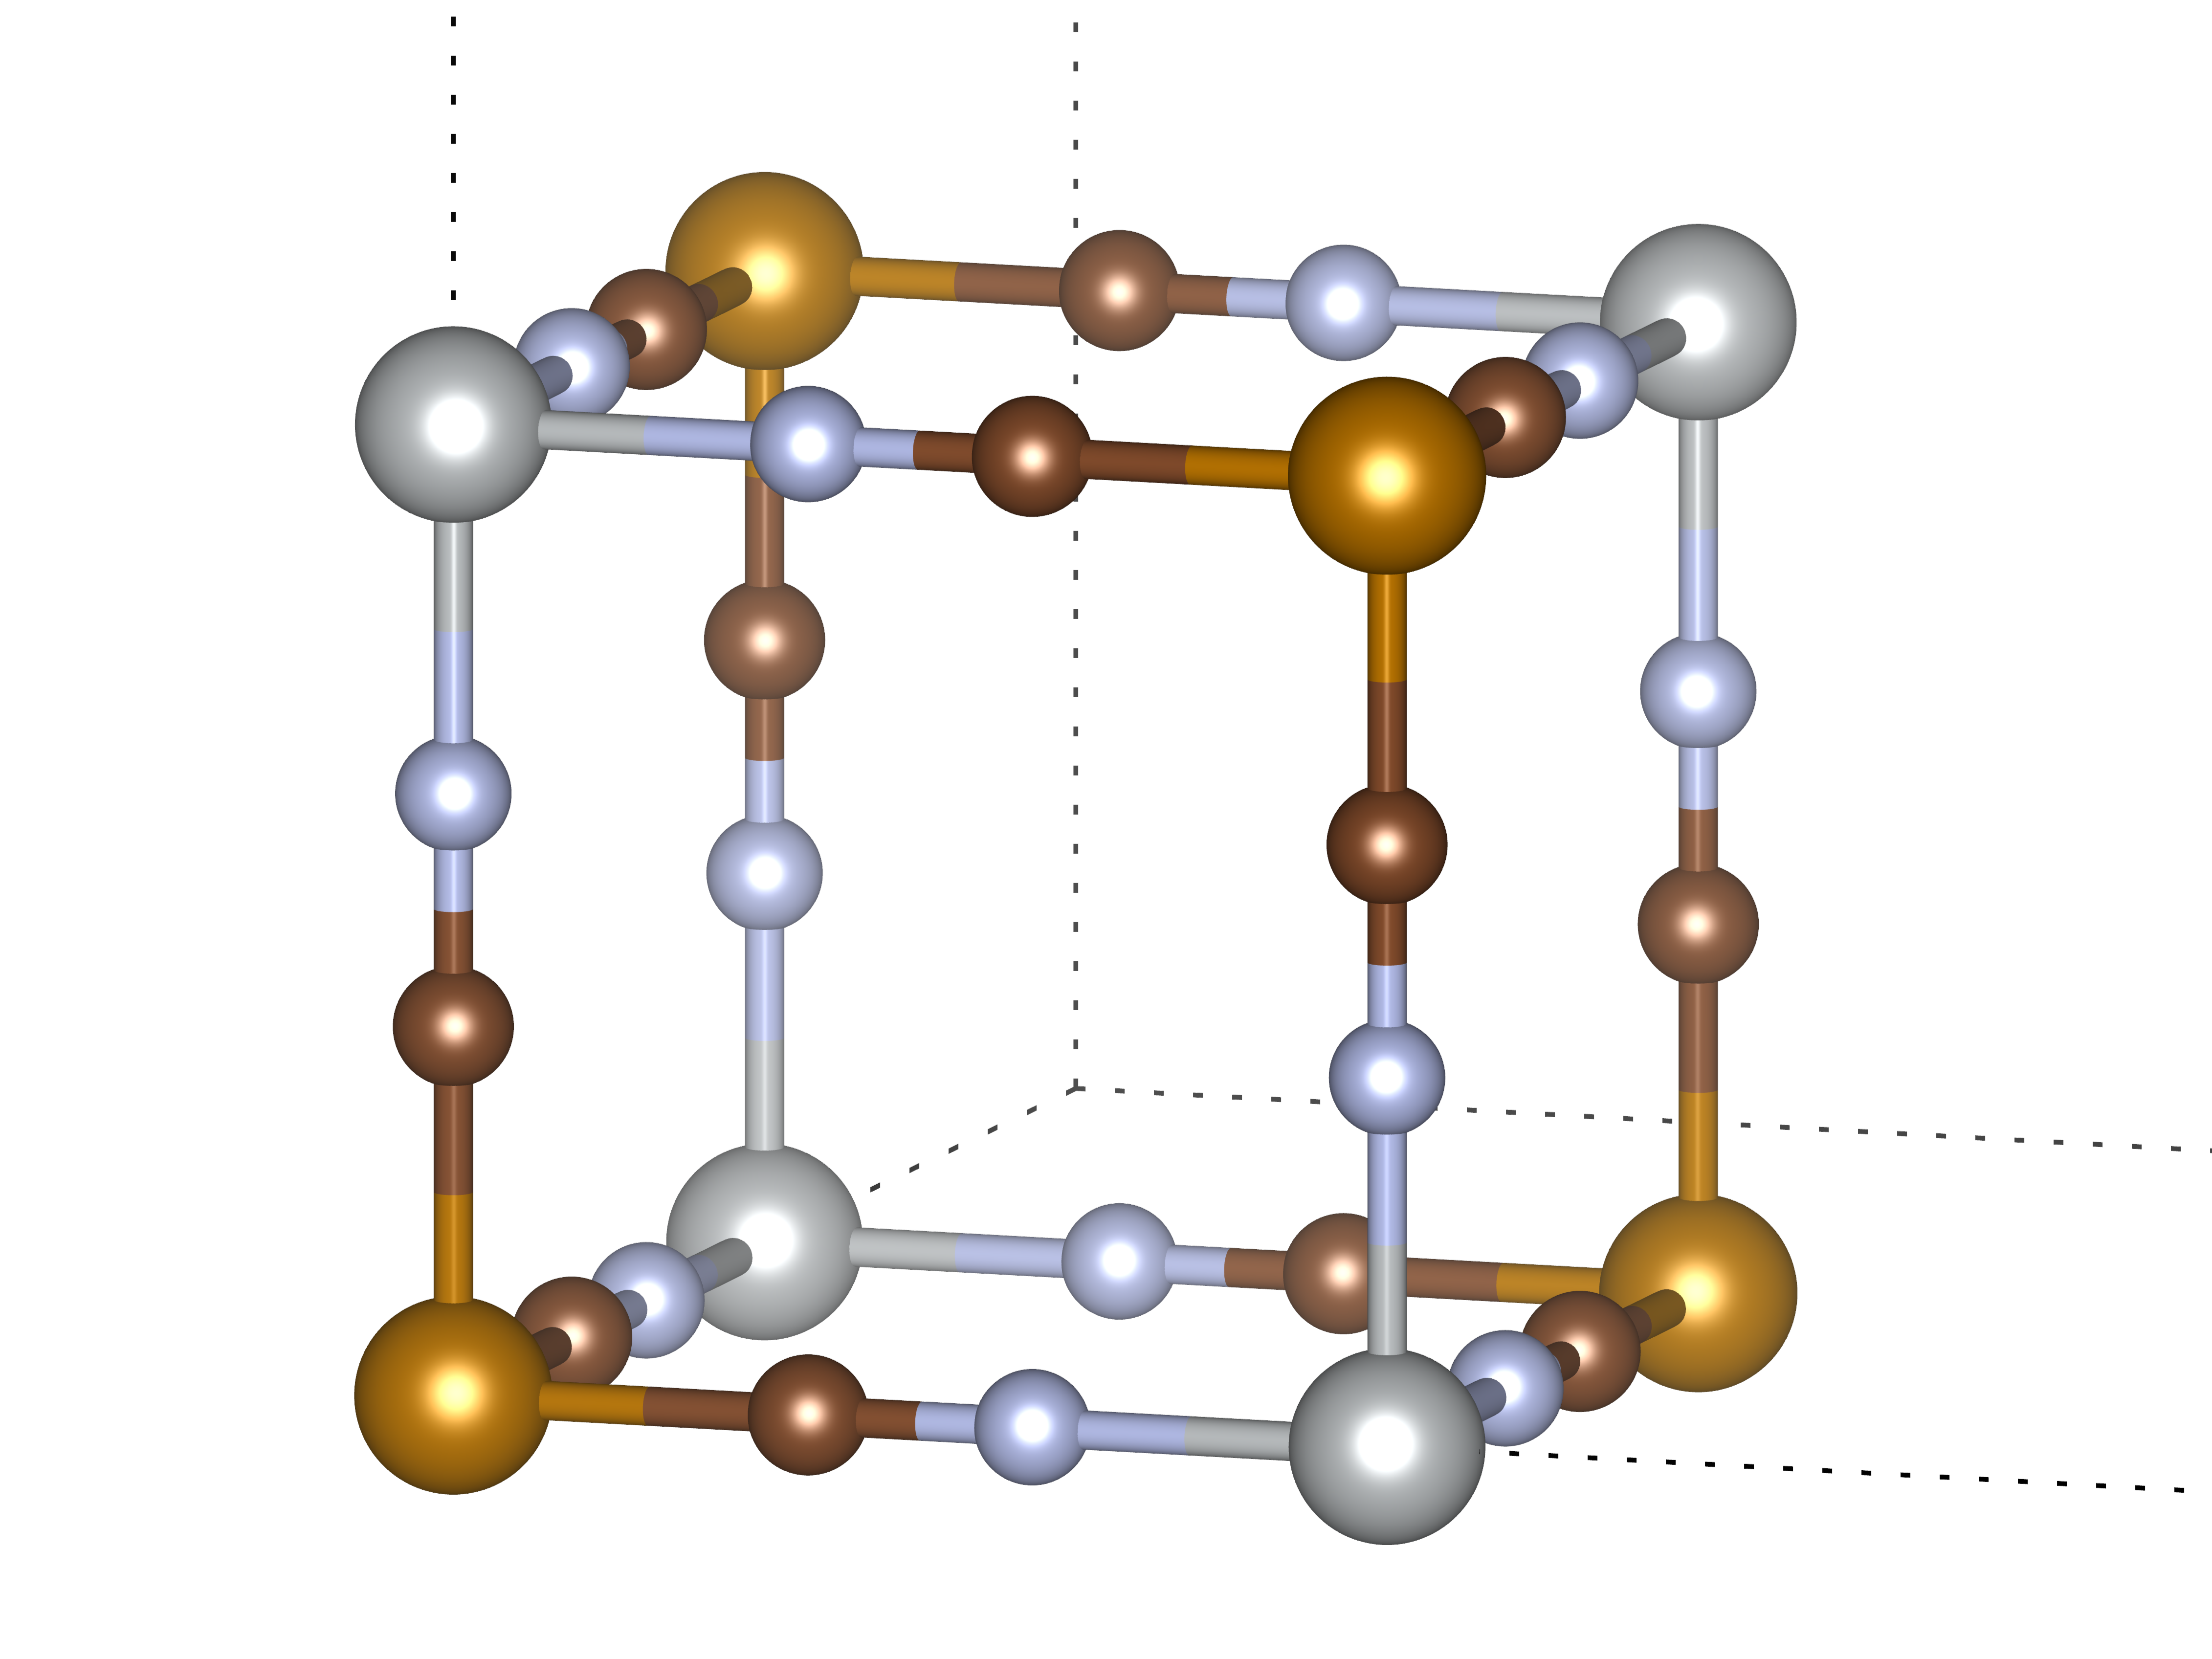
\includegraphics[scale=0.04]{Ch10/Cubic/FeCN}
	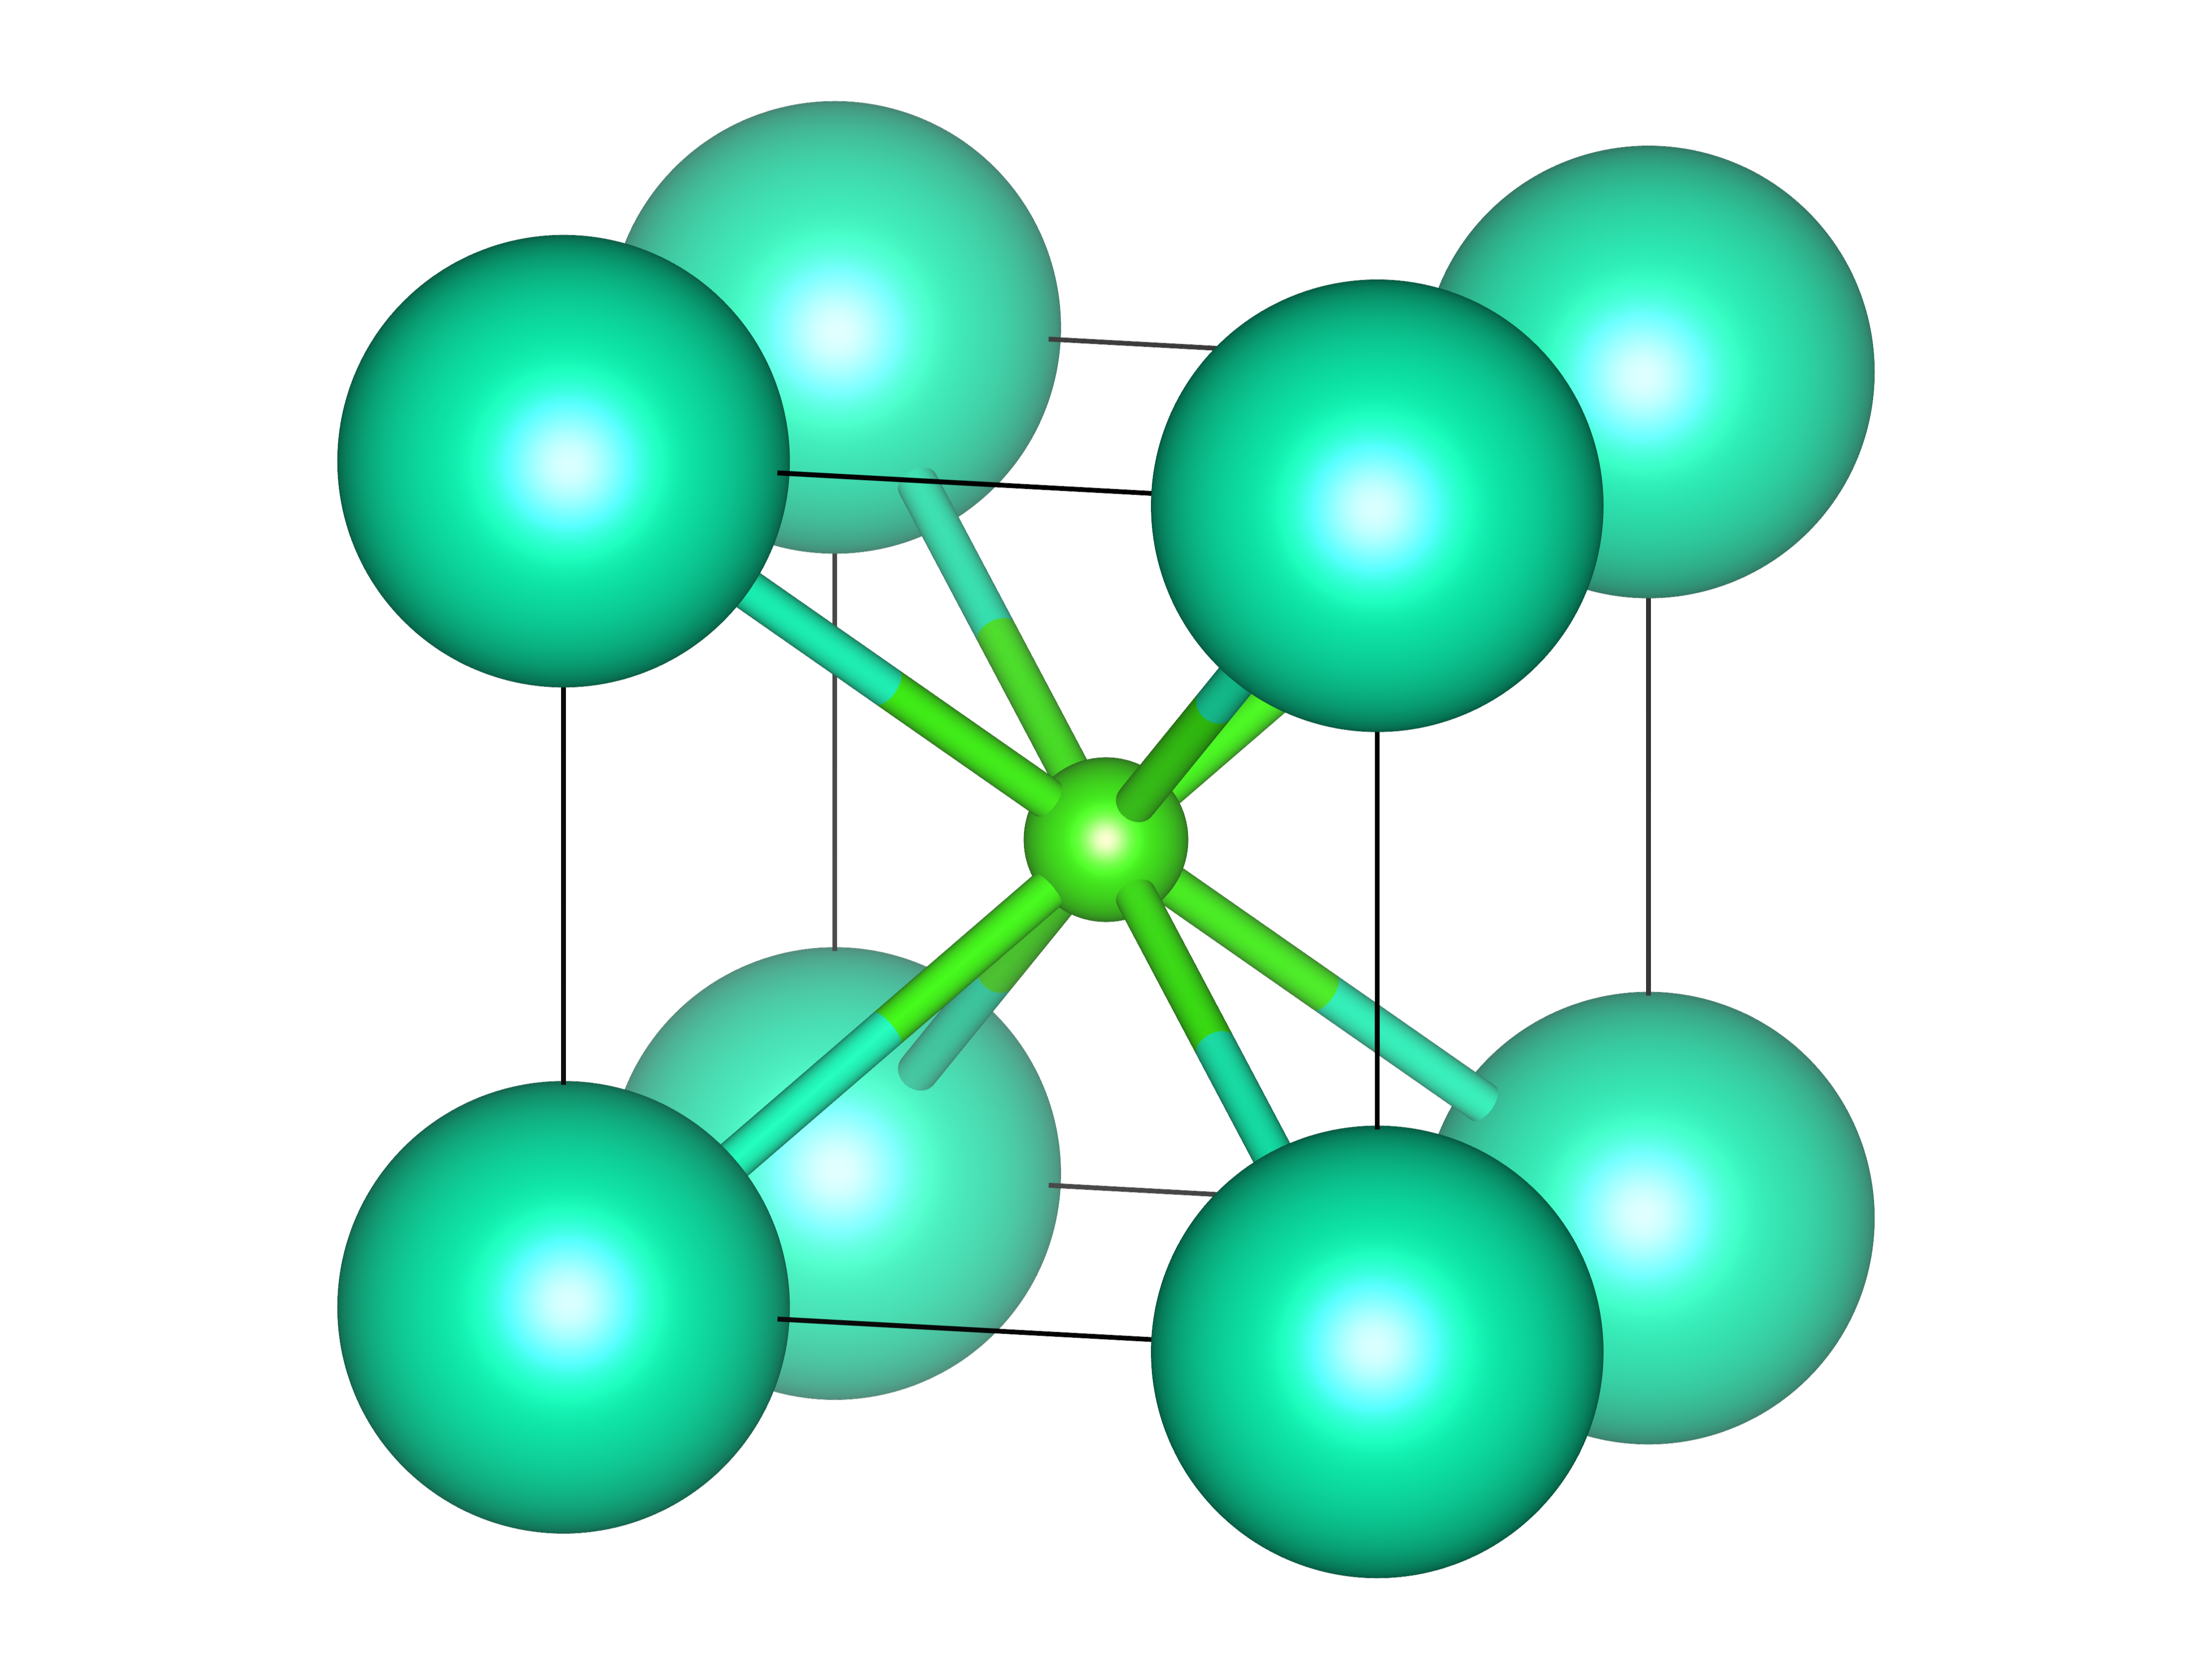
\includegraphics[scale=0.04]{Ch10/Cubic/CsCl}
	\caption{1/8 unit cell of $\rm KNiFe(CN)_6$ without K}
	\label{fecn}
	\caption{Unit cell of CsCl}
	\label{cscl}
\end{figure}
%
\subsection{Spinels and Inverse Spinels}
%
These two structures have a general formula of $\rm AB_2O_4$ where A is a divalent cation and B is a trivalent one. 
Many composite transition metal oxides take on this structure. (It's really absurd to know that $\rm Na_2WO_4$ is spinel.)
In normal spinels, O atoms stack into ccp and A atoms occupy 1/8 tetrahedral sites while B take 1/2 octahedral sites.
A conventional way of arranging unit cells is to put A on the vertices, 
then the whole cell can be considered of consisting of 4 blocks of I and II stacking as the pattern shown in figure \ref{spinel}.\\
%
\begin{figure}[h]
	\centering
	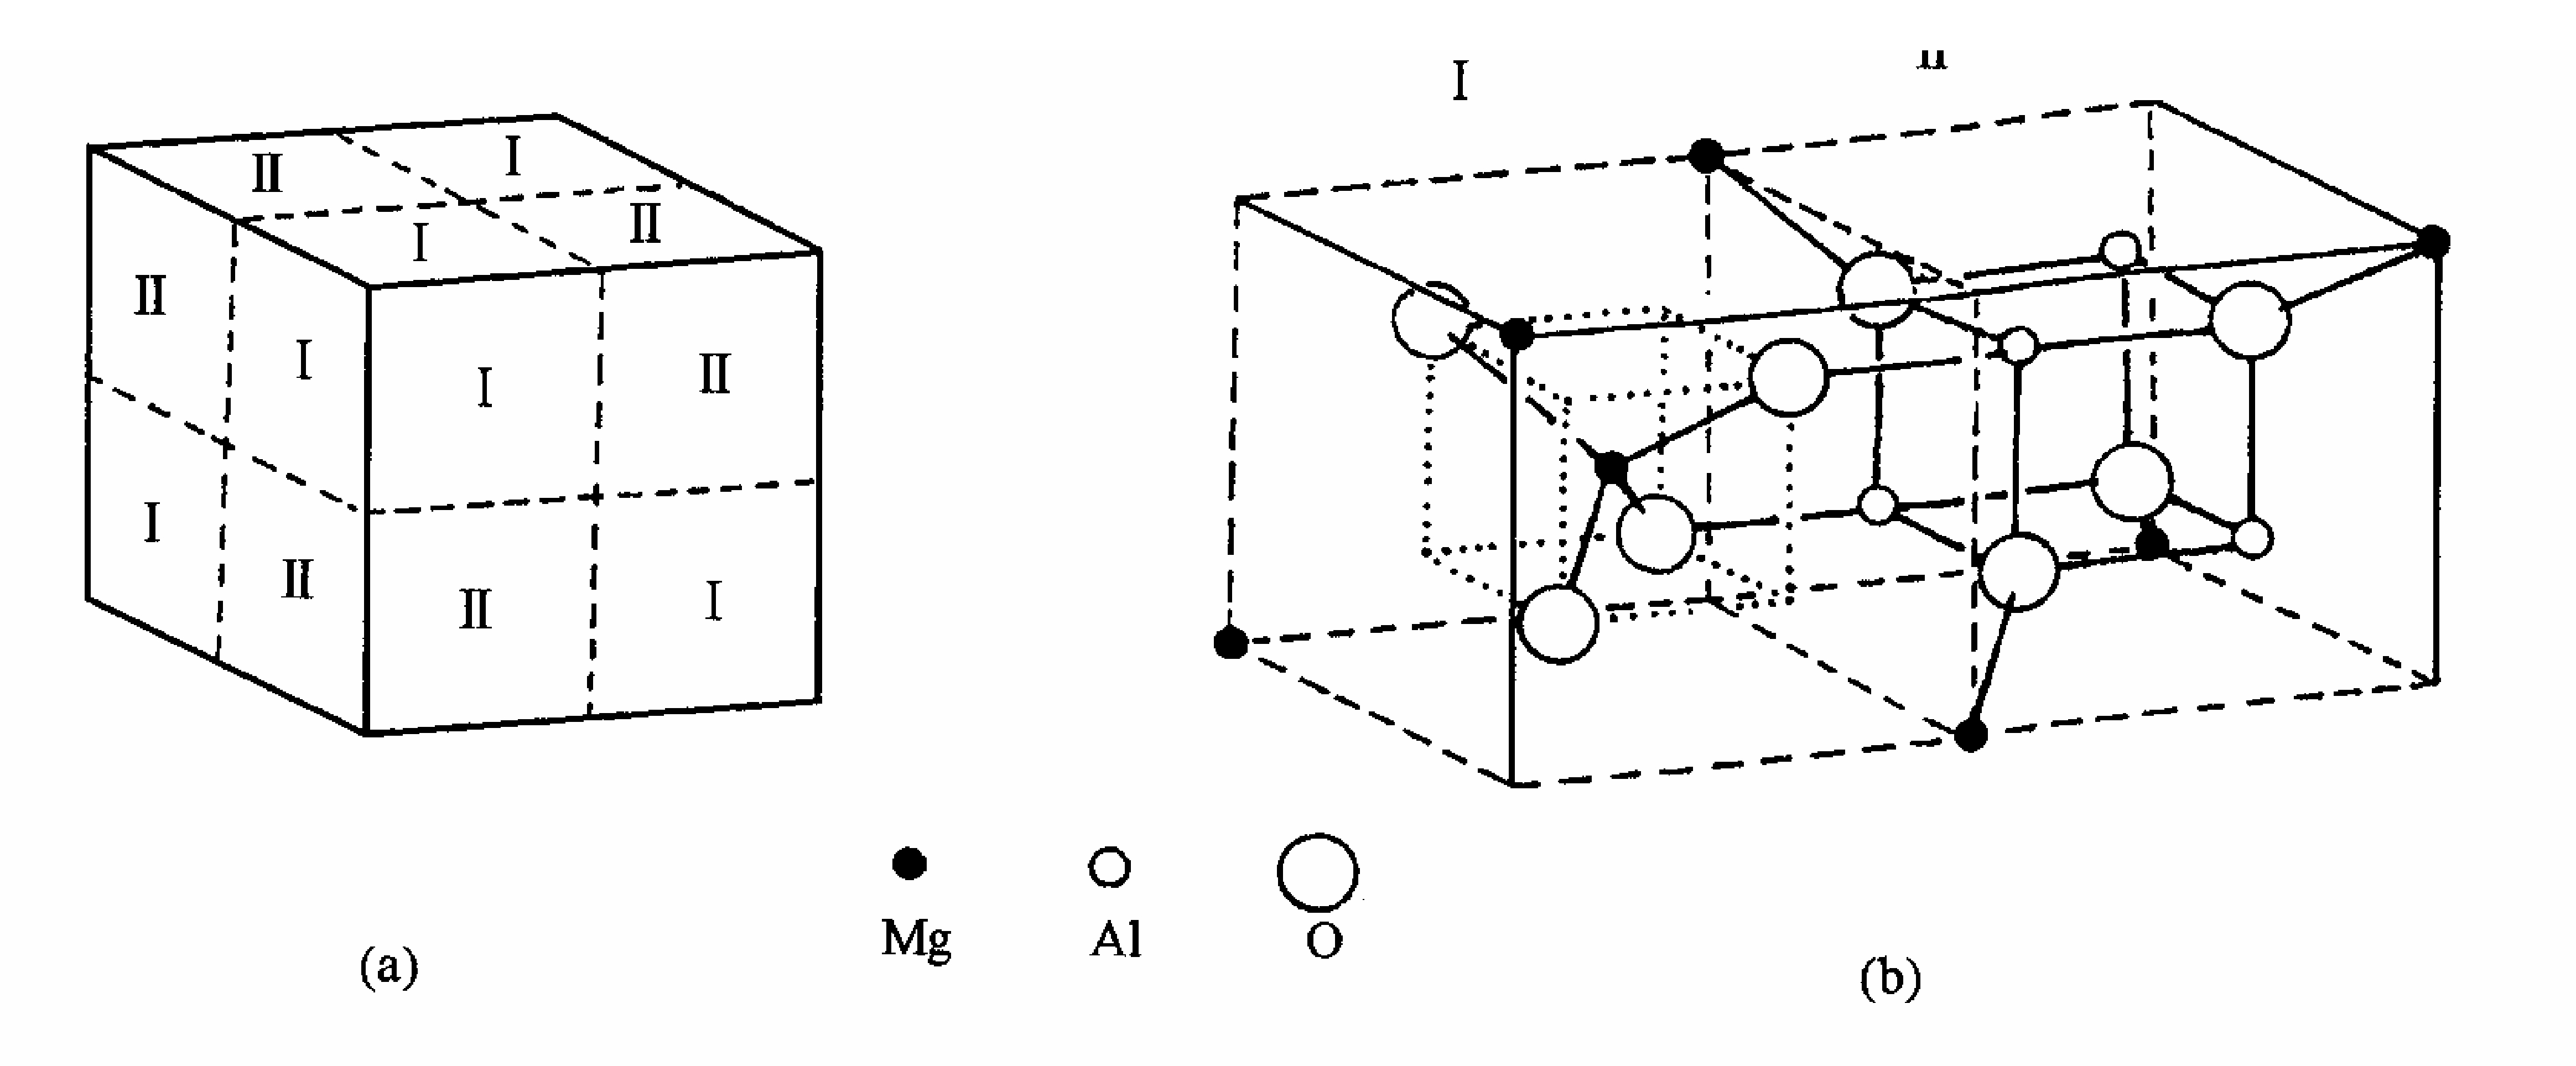
\includegraphics[scale=0.06]{Ch10/Spinel/spinel}
	\caption{Stacking of spinel structure}
	\label{spinel}
\end{figure}\\
%
In block II, four $\rm [BO_6]$ octahedra, each sharing three edges with another three octahedra, forms a $\rm [B_4O_4]$ cube. 
Four tetrahedrally placed cubes then form another cube in between. 
Within this framework every B atom is a shared vertex of two cubes, every cube links 2 upper and 2 lower cubes. 
Every O atom, up to now bound to 3 B atoms and shared by 3 $\rm [BO_6]$ octahedra, is also a vertex of $\rm [AO_4]$ tetrahedron.
Therefore, the coordination is $\rm [BO_6]$, $\rm [AO_4]$ and $\rm [OAB_3]$, with all the atoms only one chemical environment.
This description is illustrated in figure \ref{spinel framework}. If we scan through the structure from bottom to top, 
we can draw the alignment of atoms in different height, shown in figure \ref{spl}.\\
%
\begin{figure}[h]
	\centering
	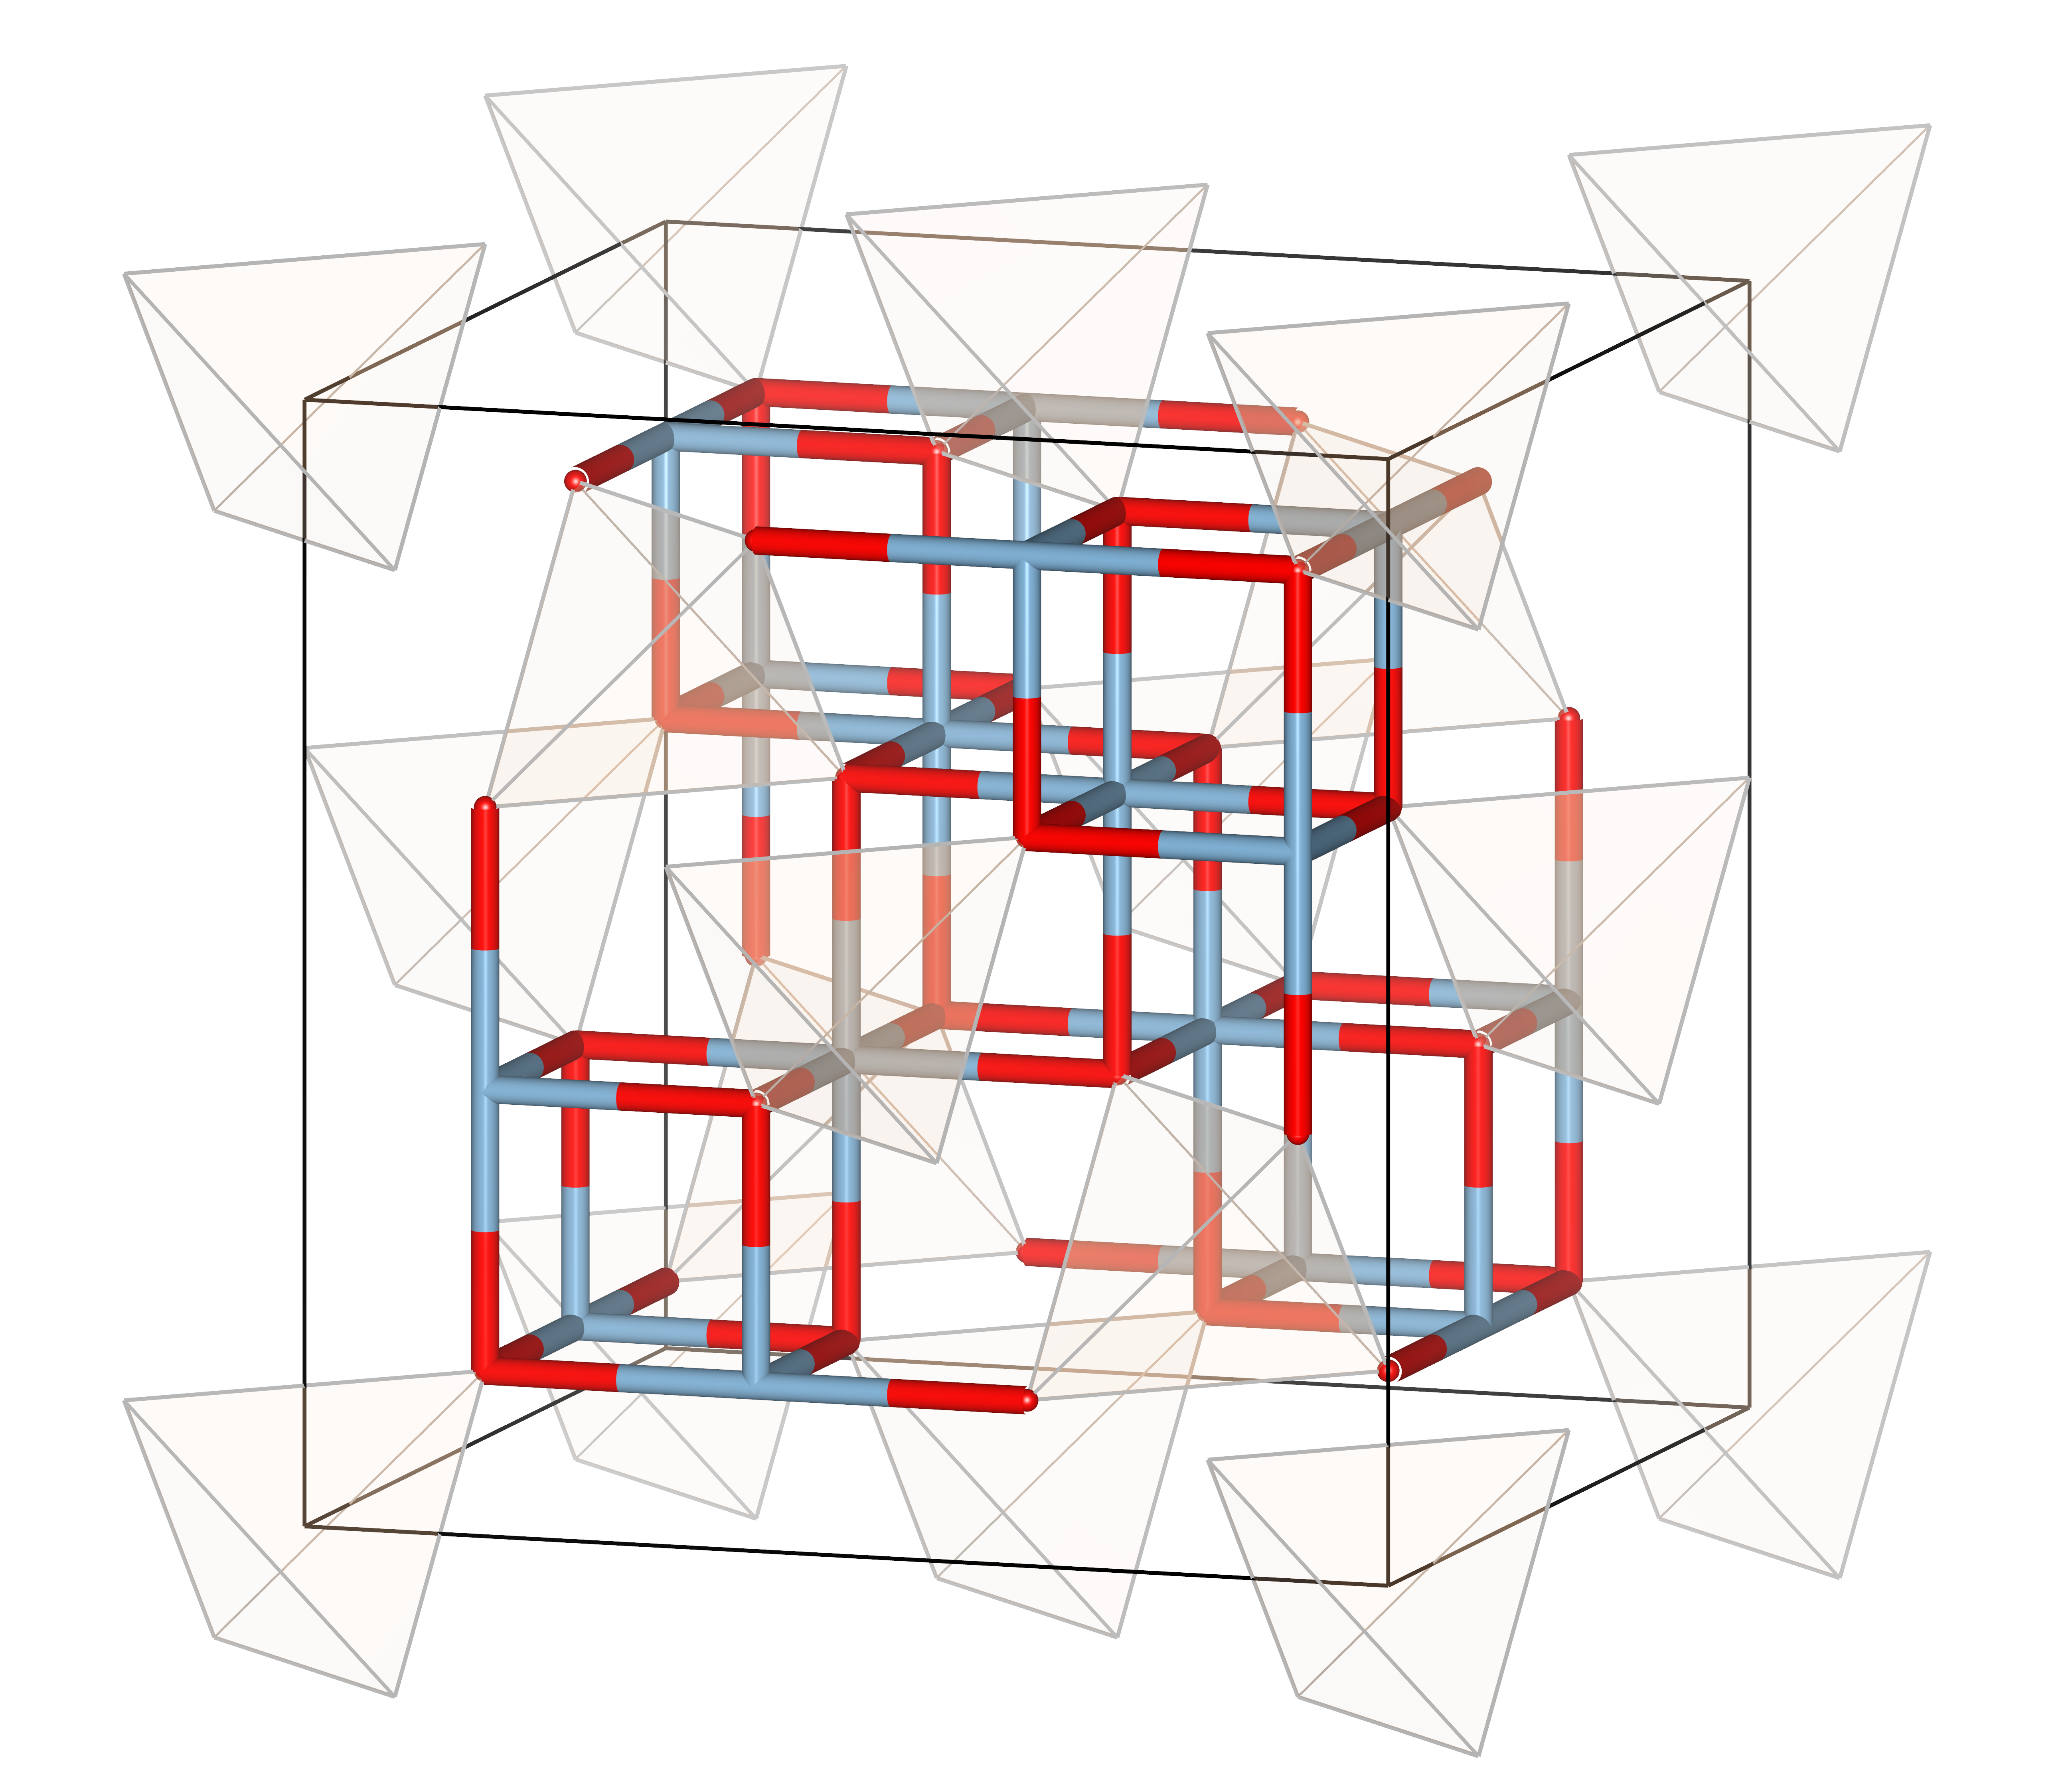
\includegraphics[scale=0.042]{Ch10/Spinel/spinel_framework}
	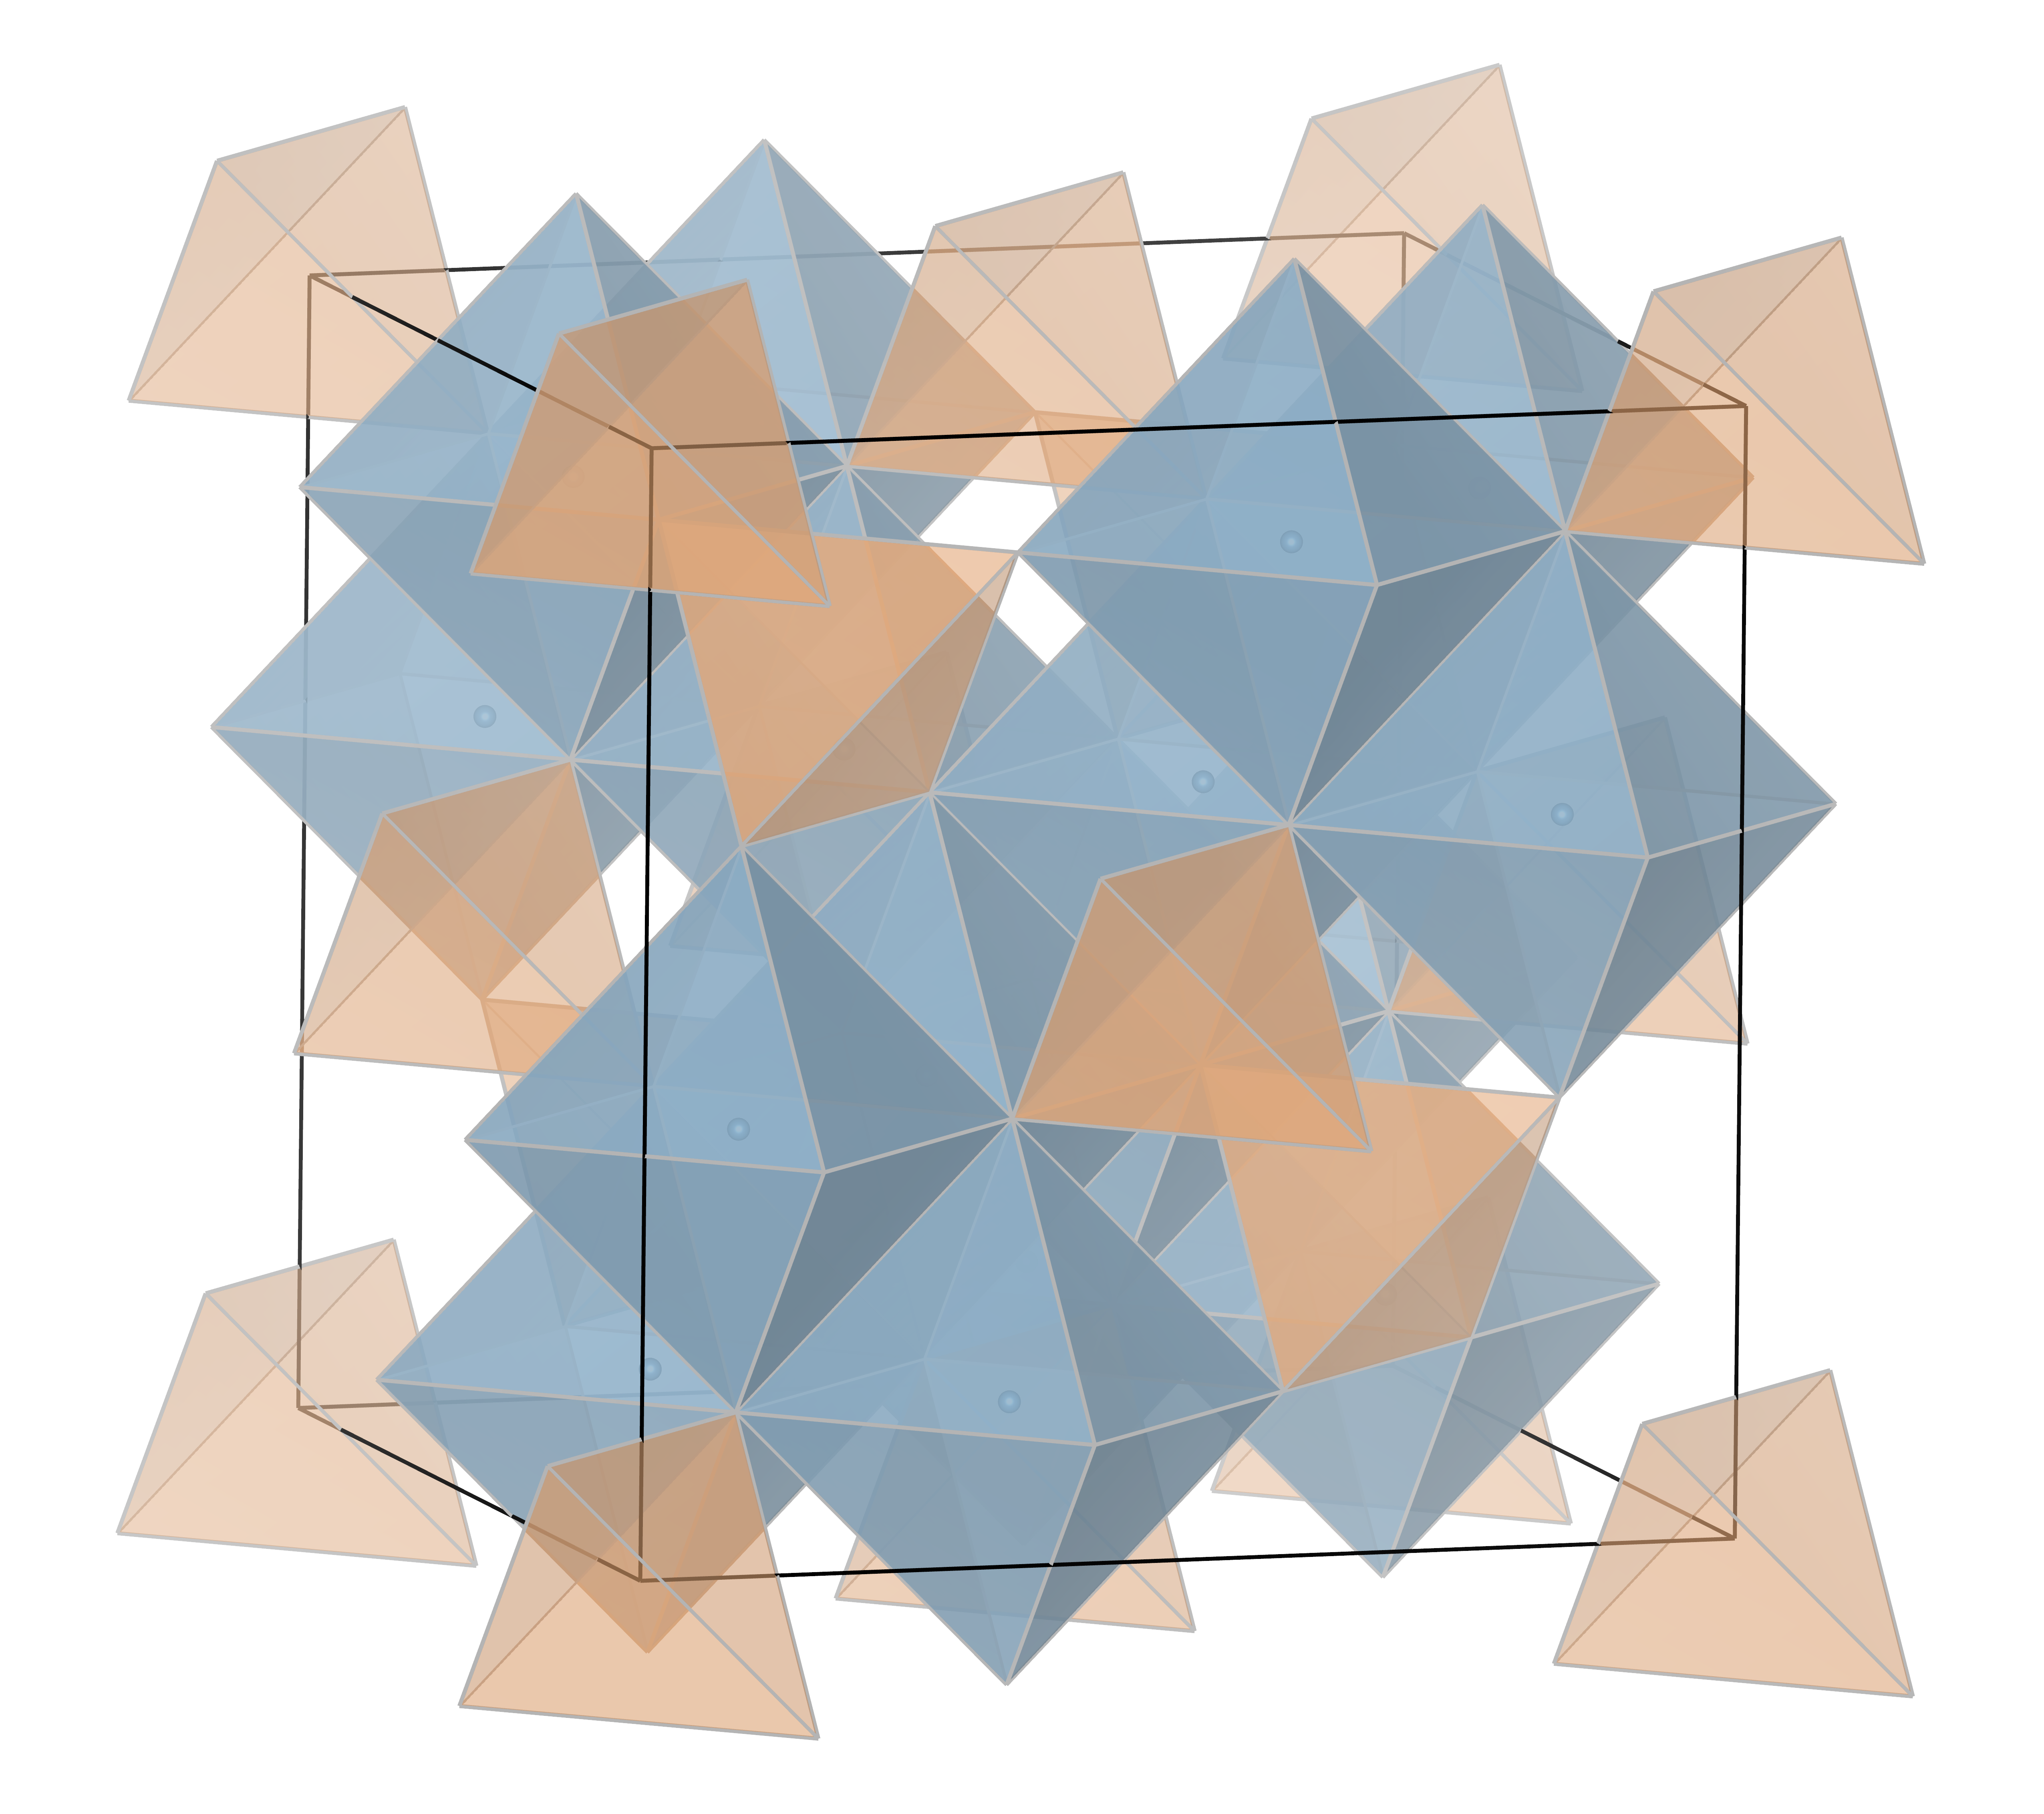
\includegraphics[scale=0.04]{Ch10/Spinel/spinel_polyhedra}
	\caption{Polyhedra description of spinel structure}
	\label{spinel framework}
	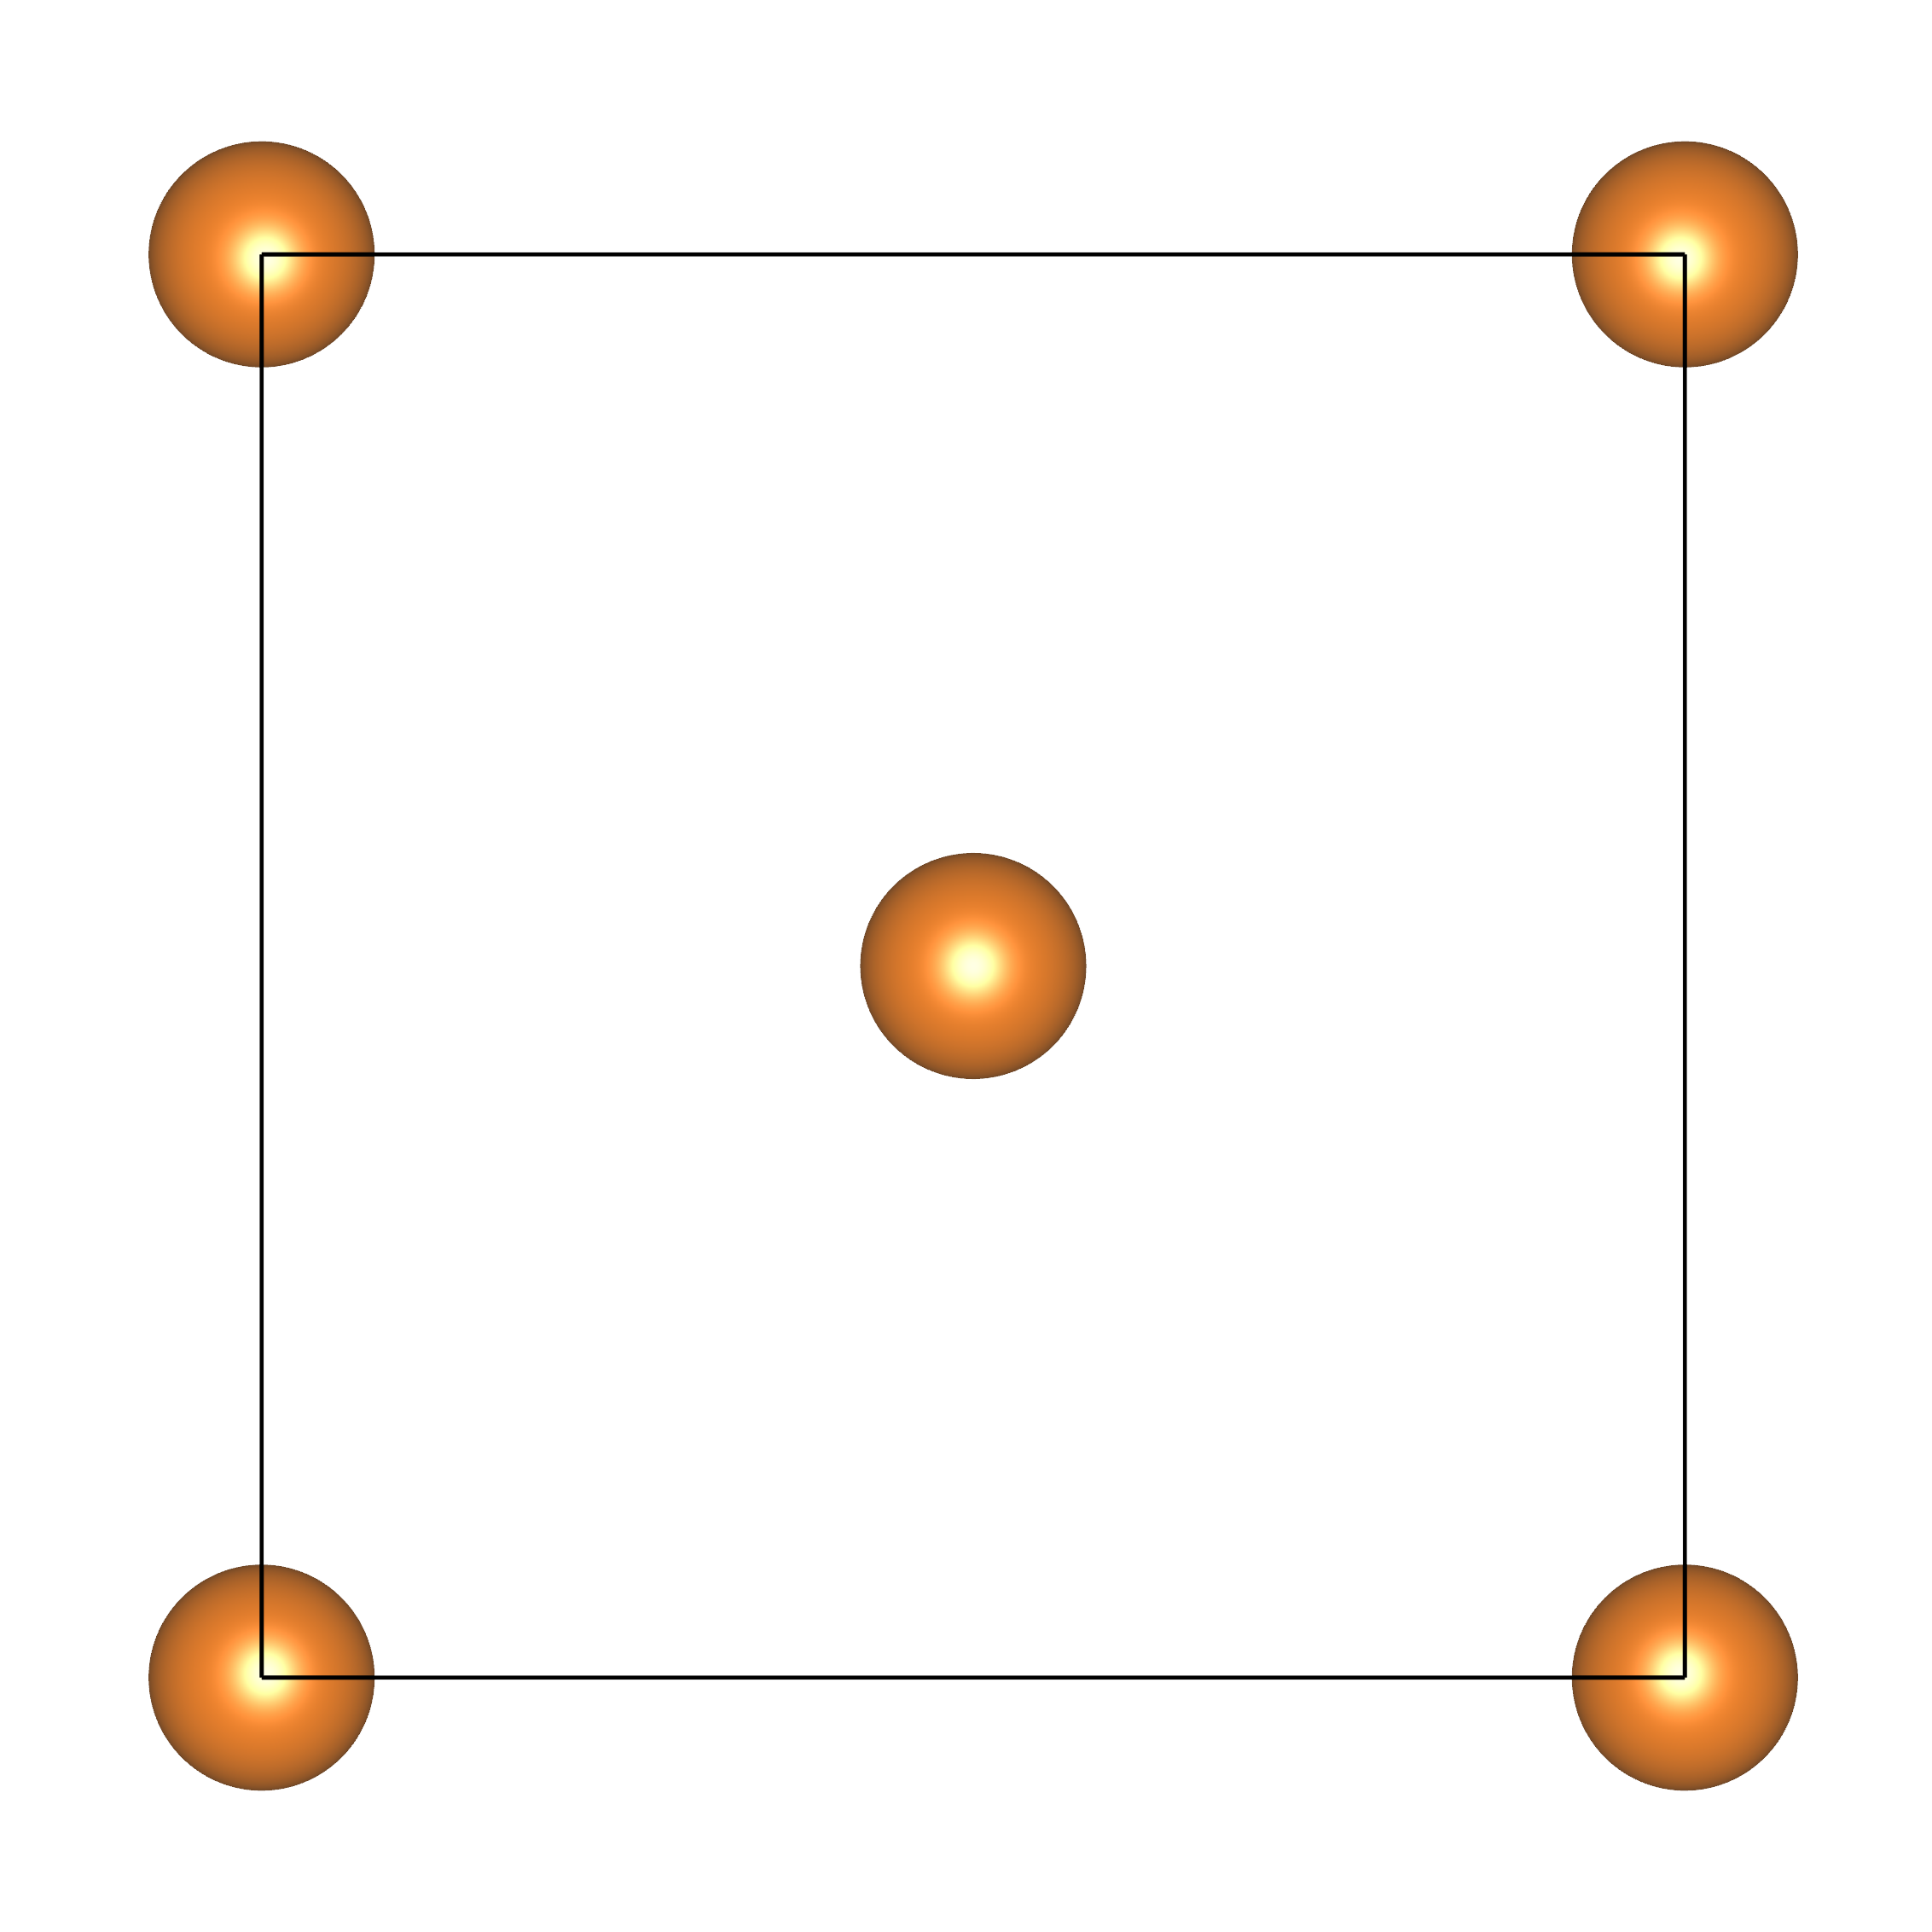
\includegraphics[scale=0.03]{Ch10/Spinel/spl0}
	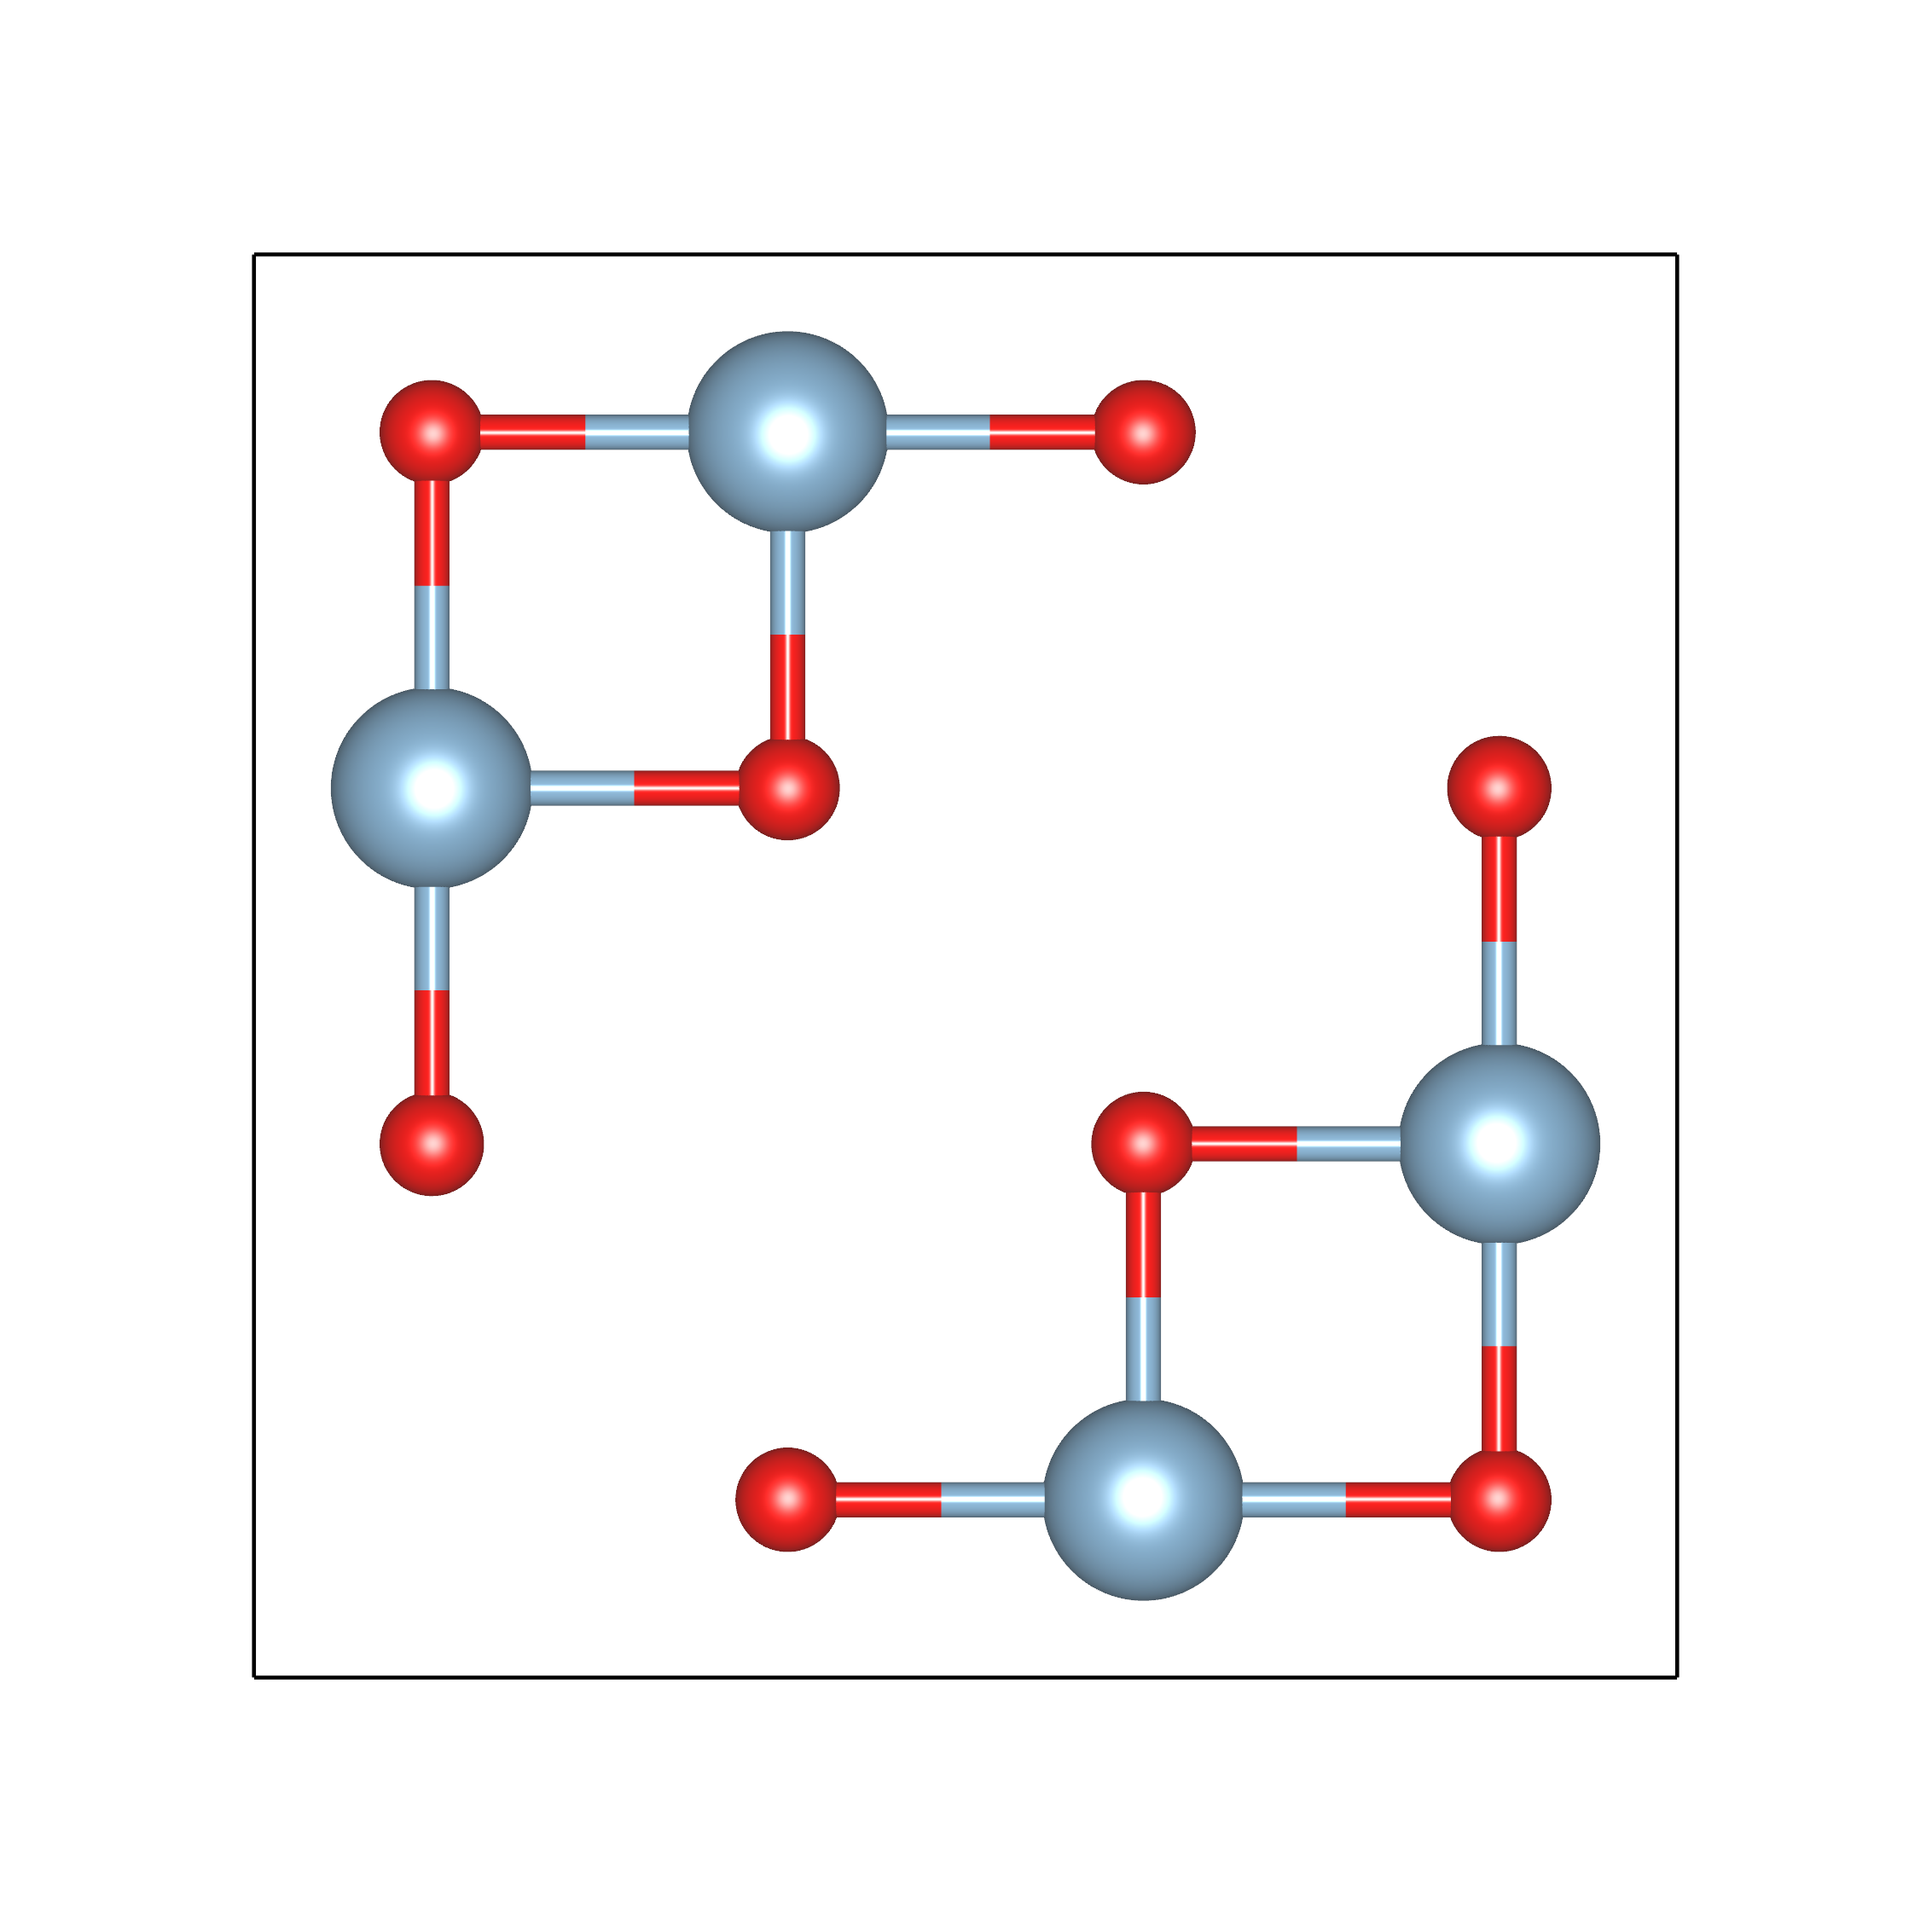
\includegraphics[scale=0.03]{Ch10/Spinel/spl1}
	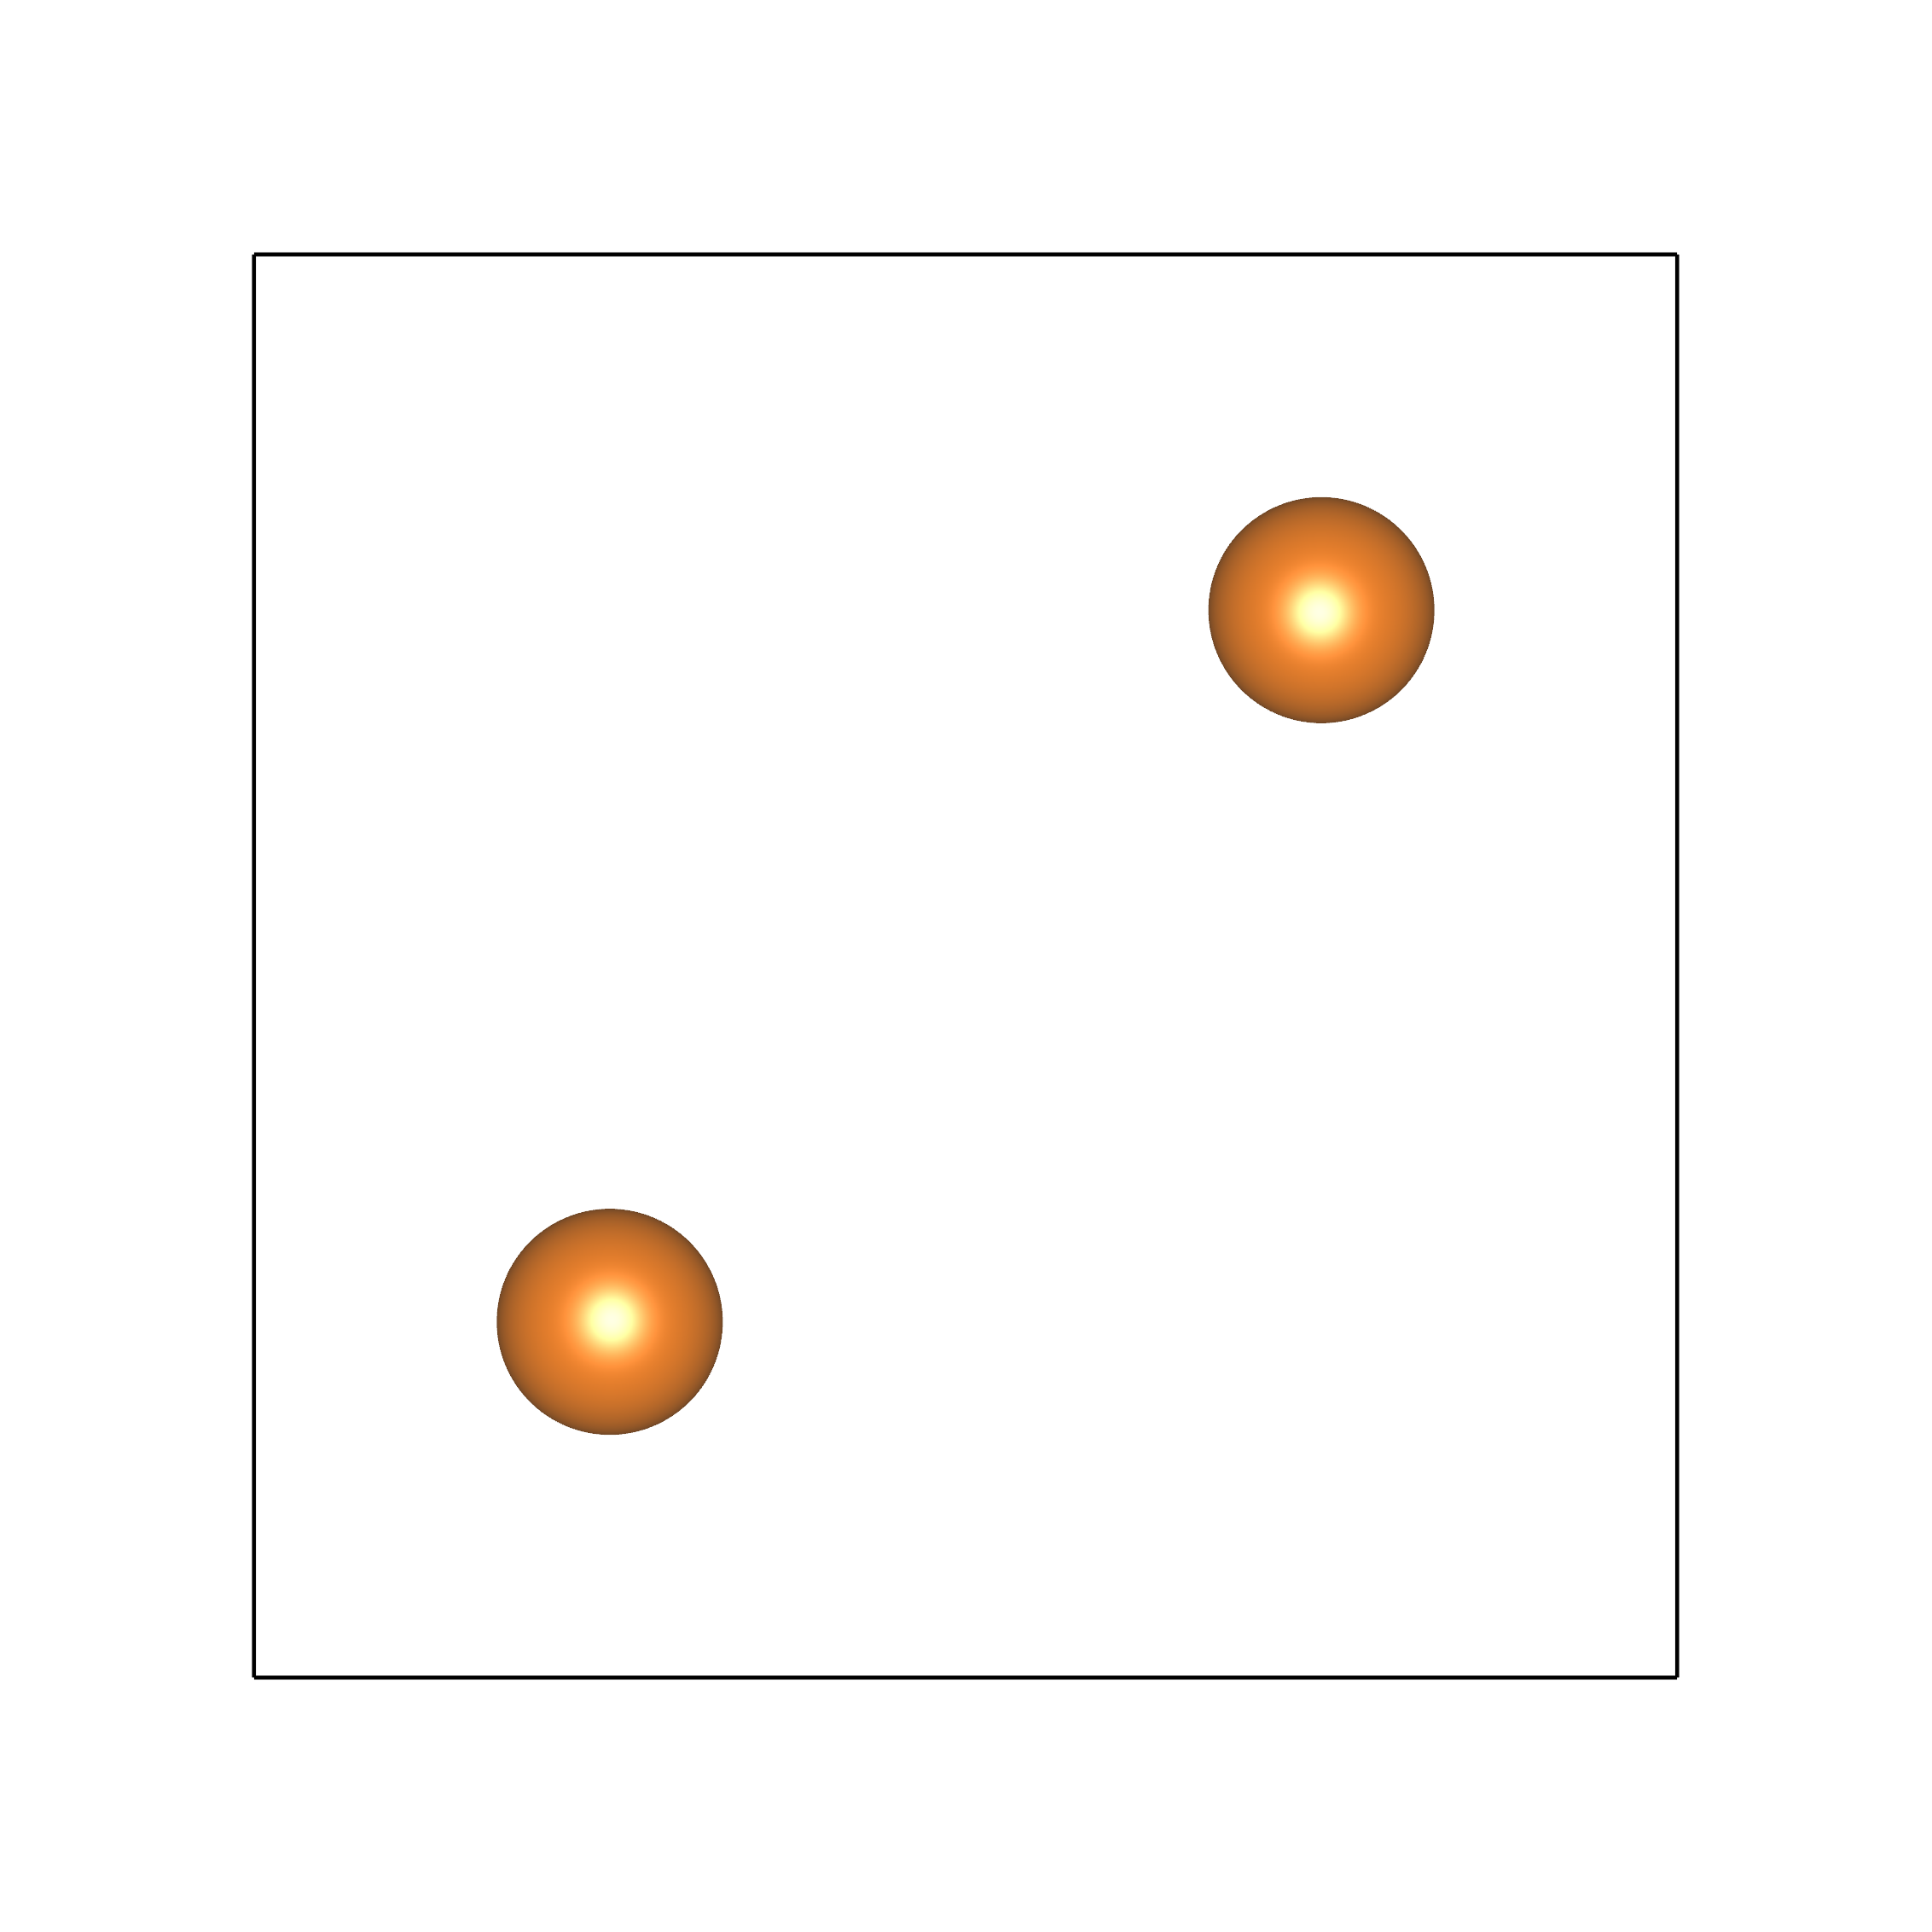
\includegraphics[scale=0.03]{Ch10/Spinel/spl2}
	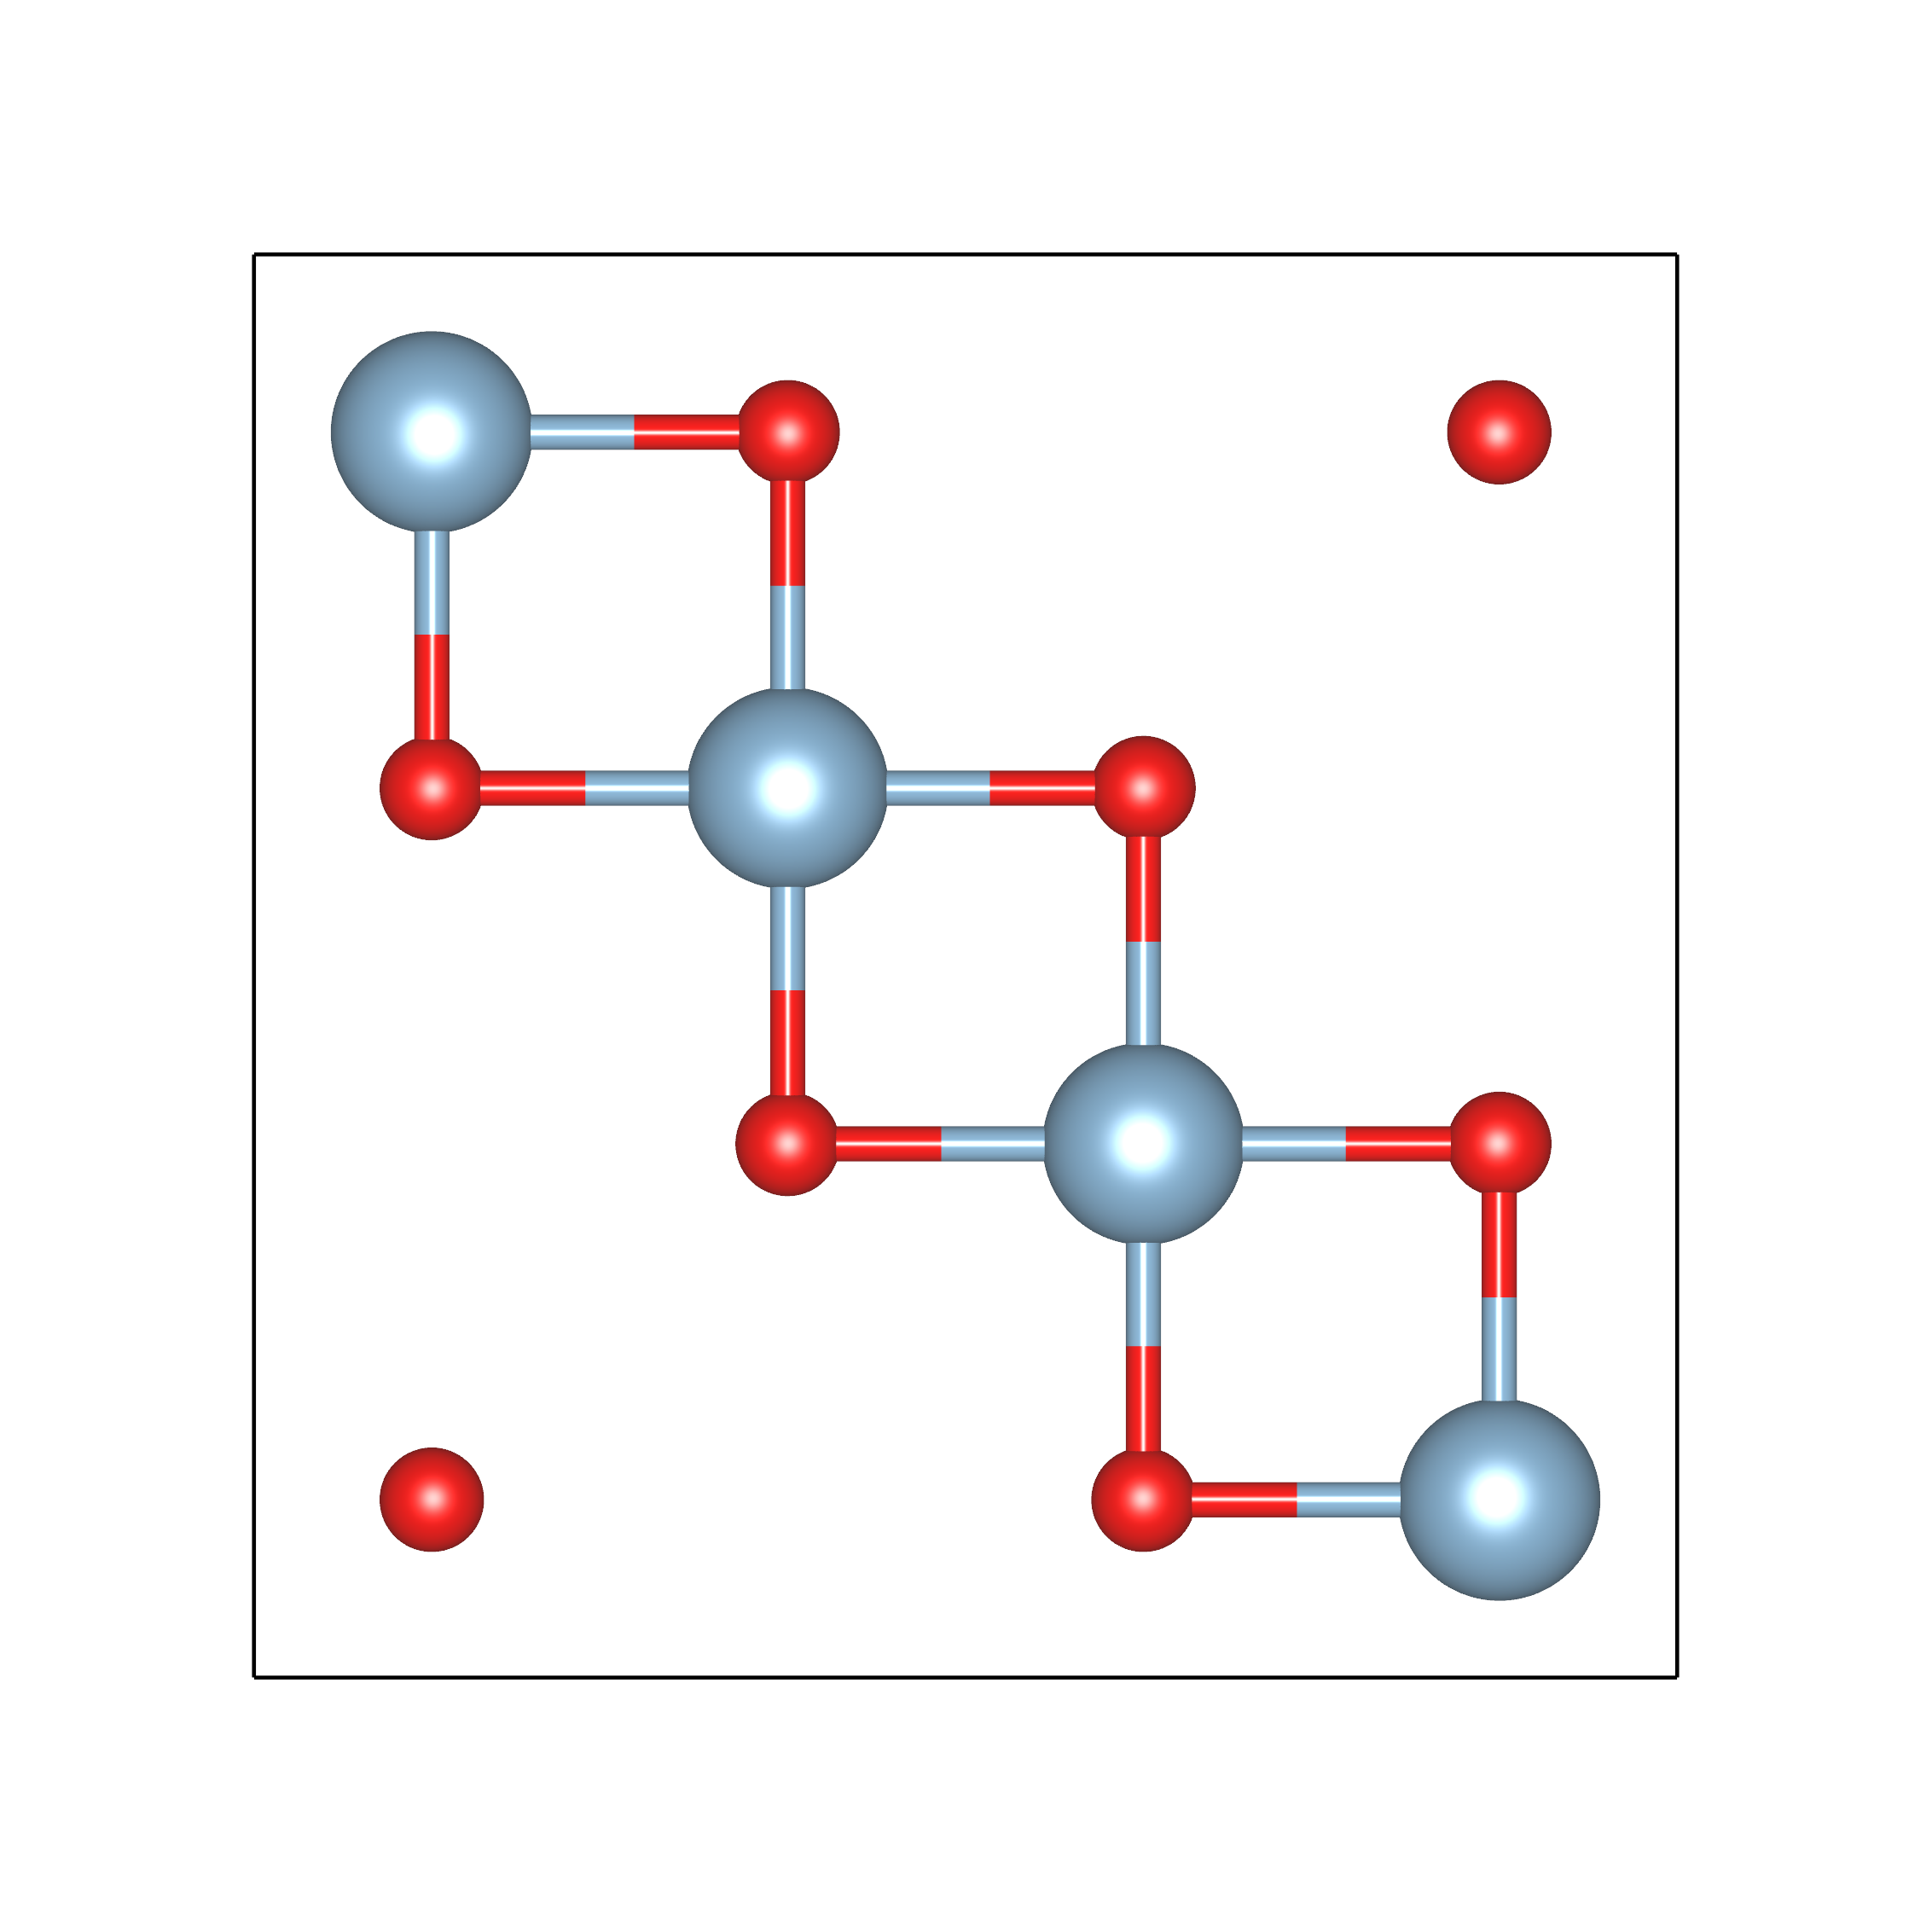
\includegraphics[scale=0.03]{Ch10/Spinel/spl3}
	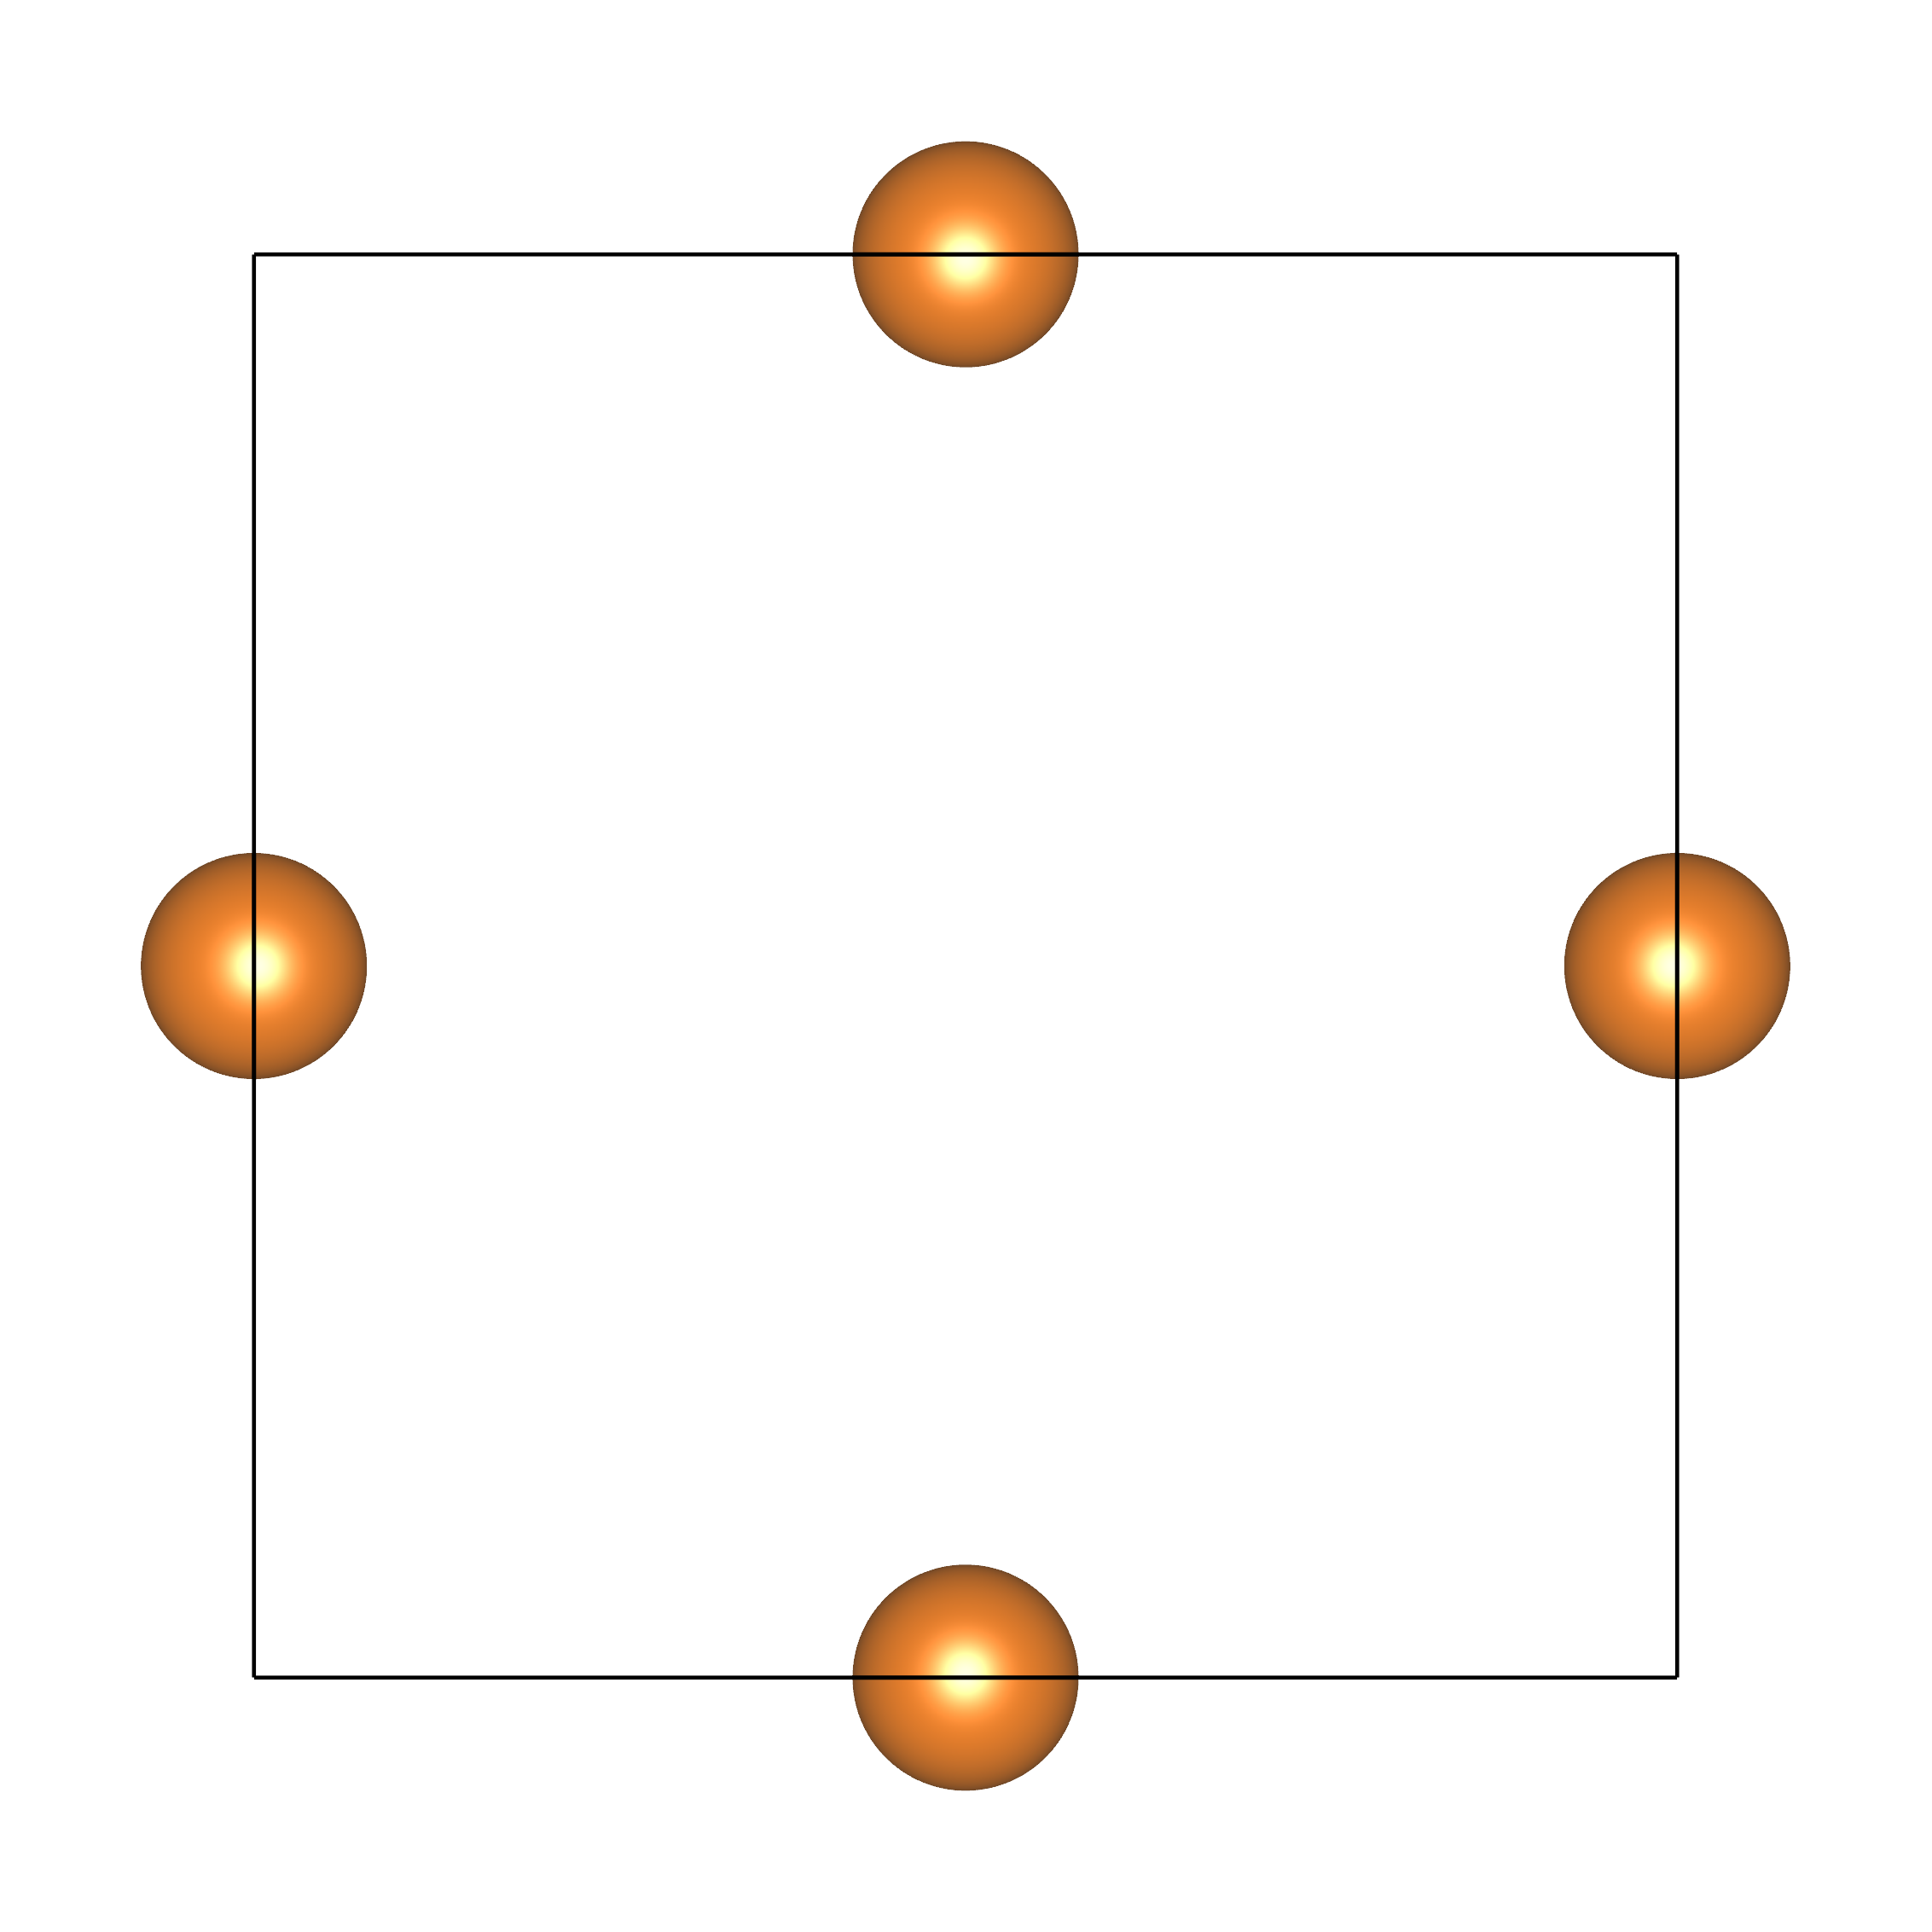
\includegraphics[scale=0.03]{Ch10/Spinel/spl4}
	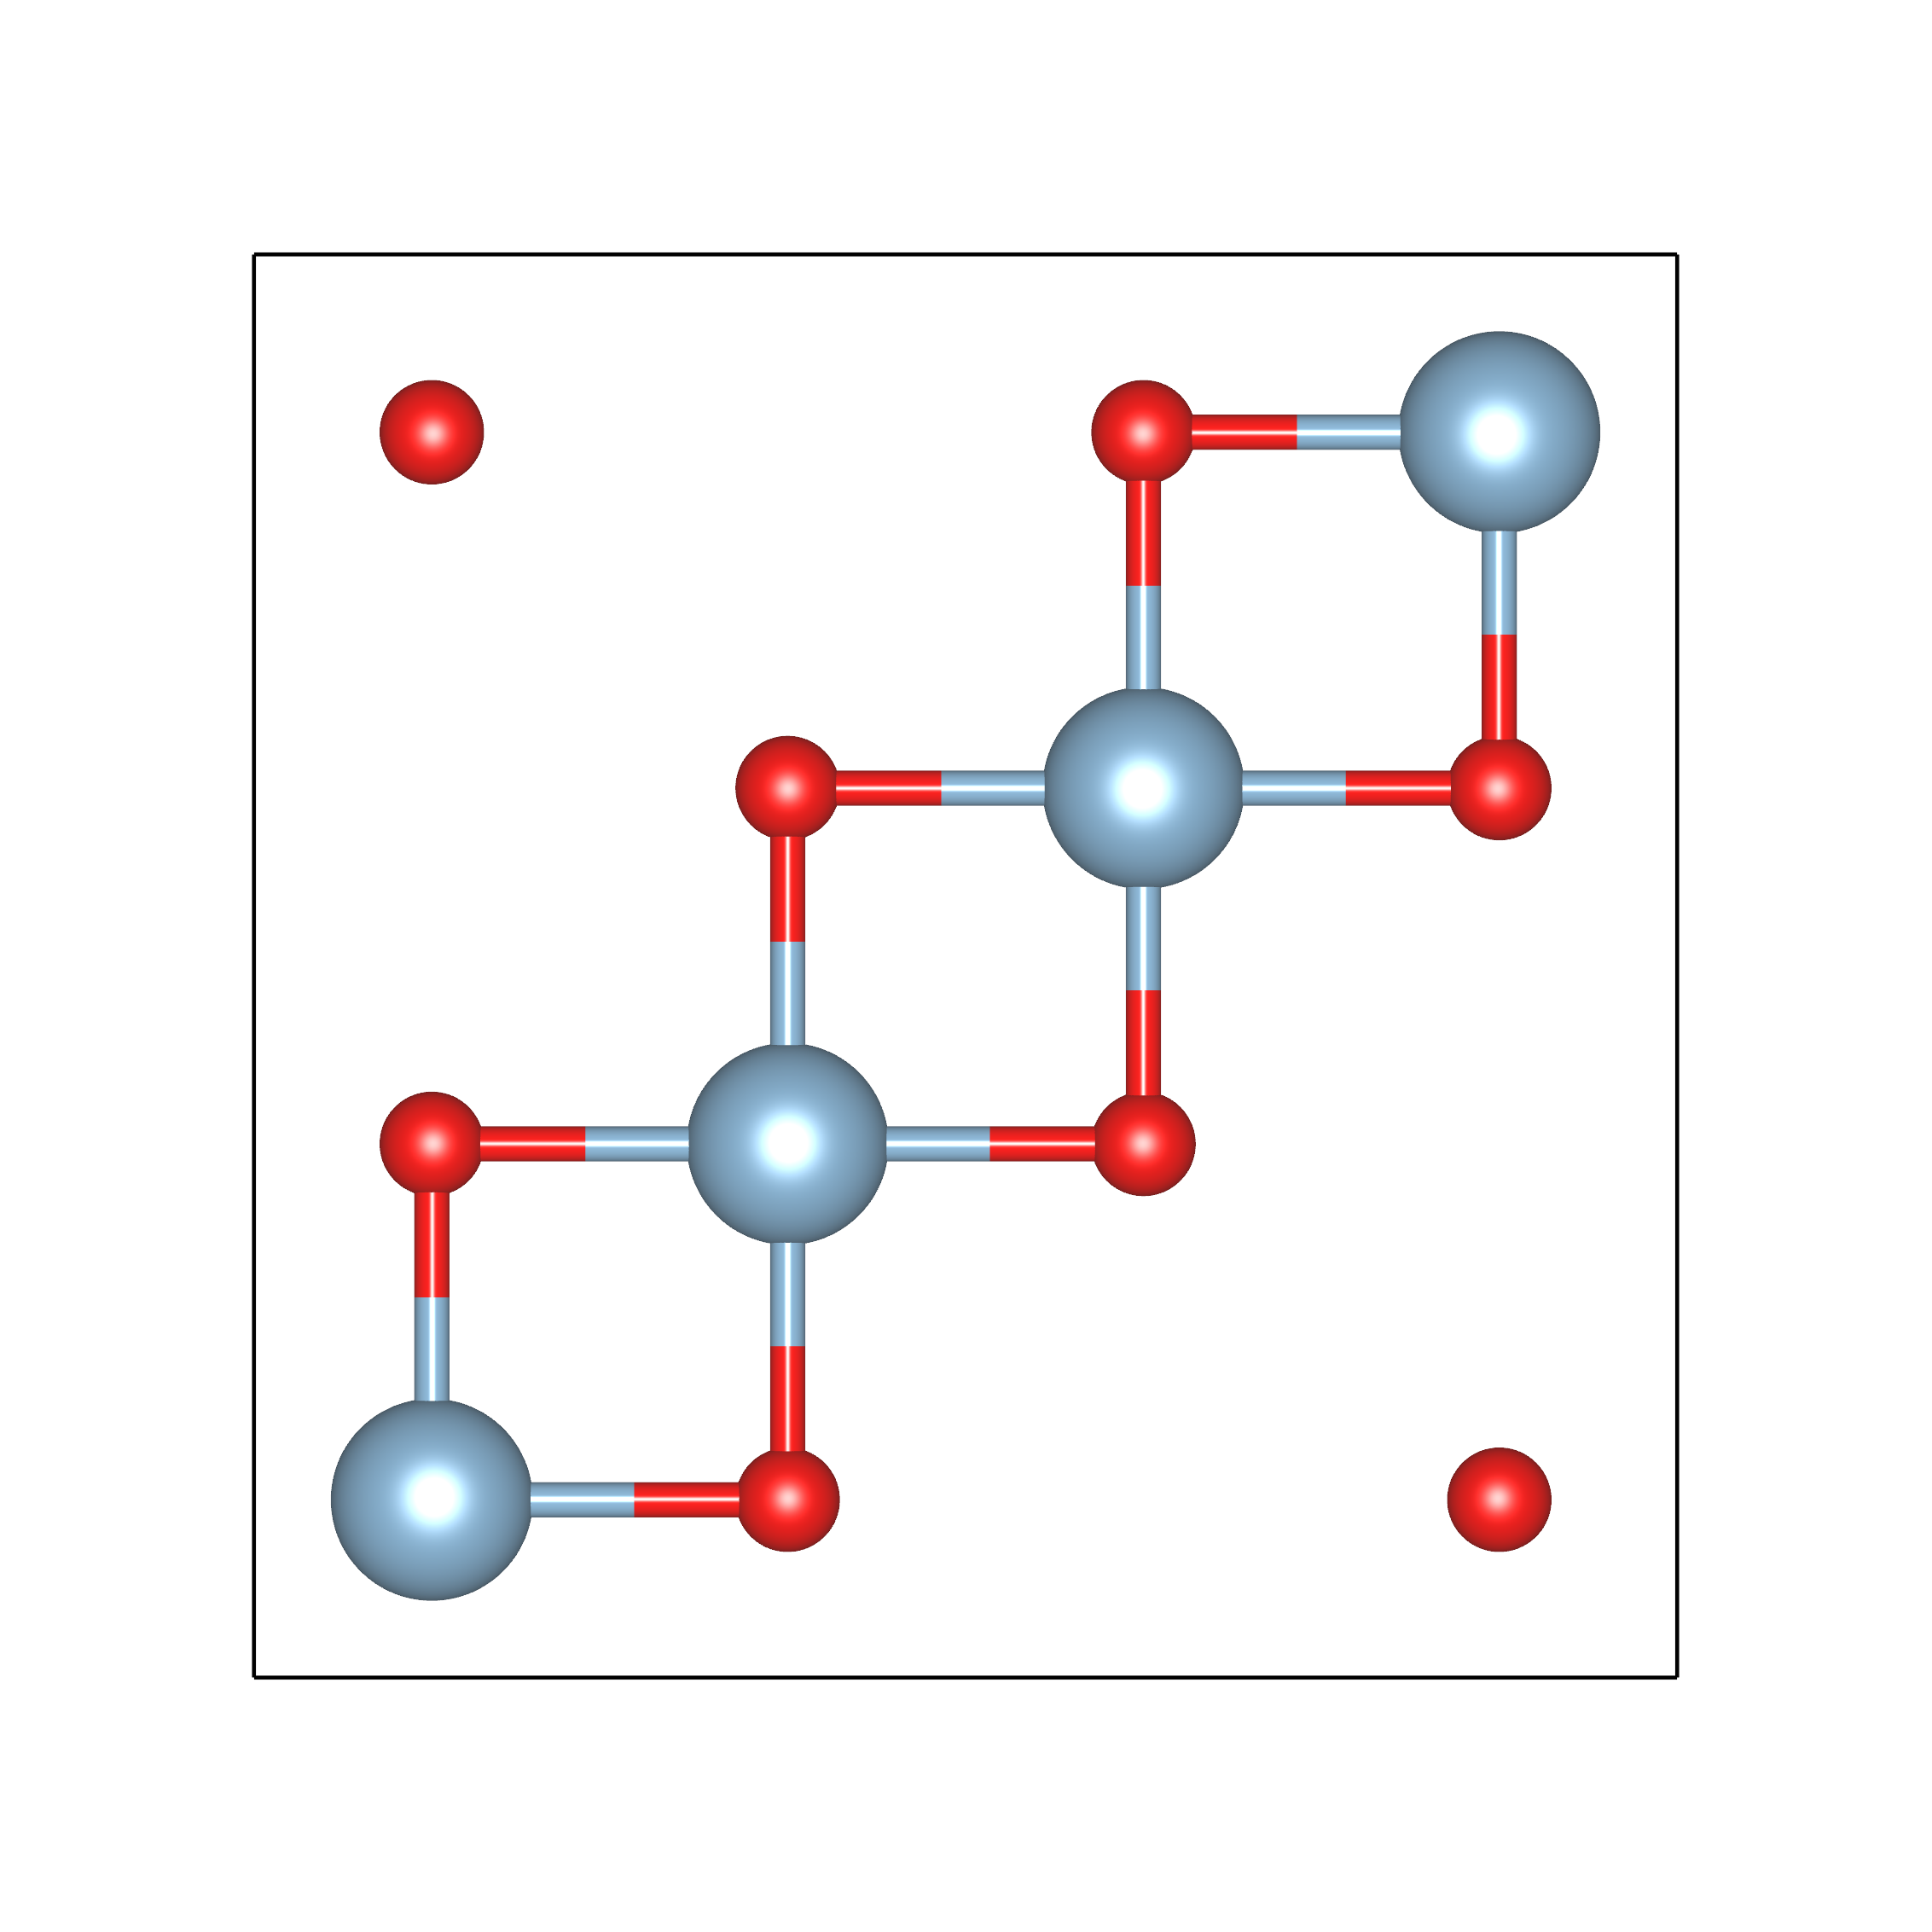
\includegraphics[scale=0.03]{Ch10/Spinel/spl5}
	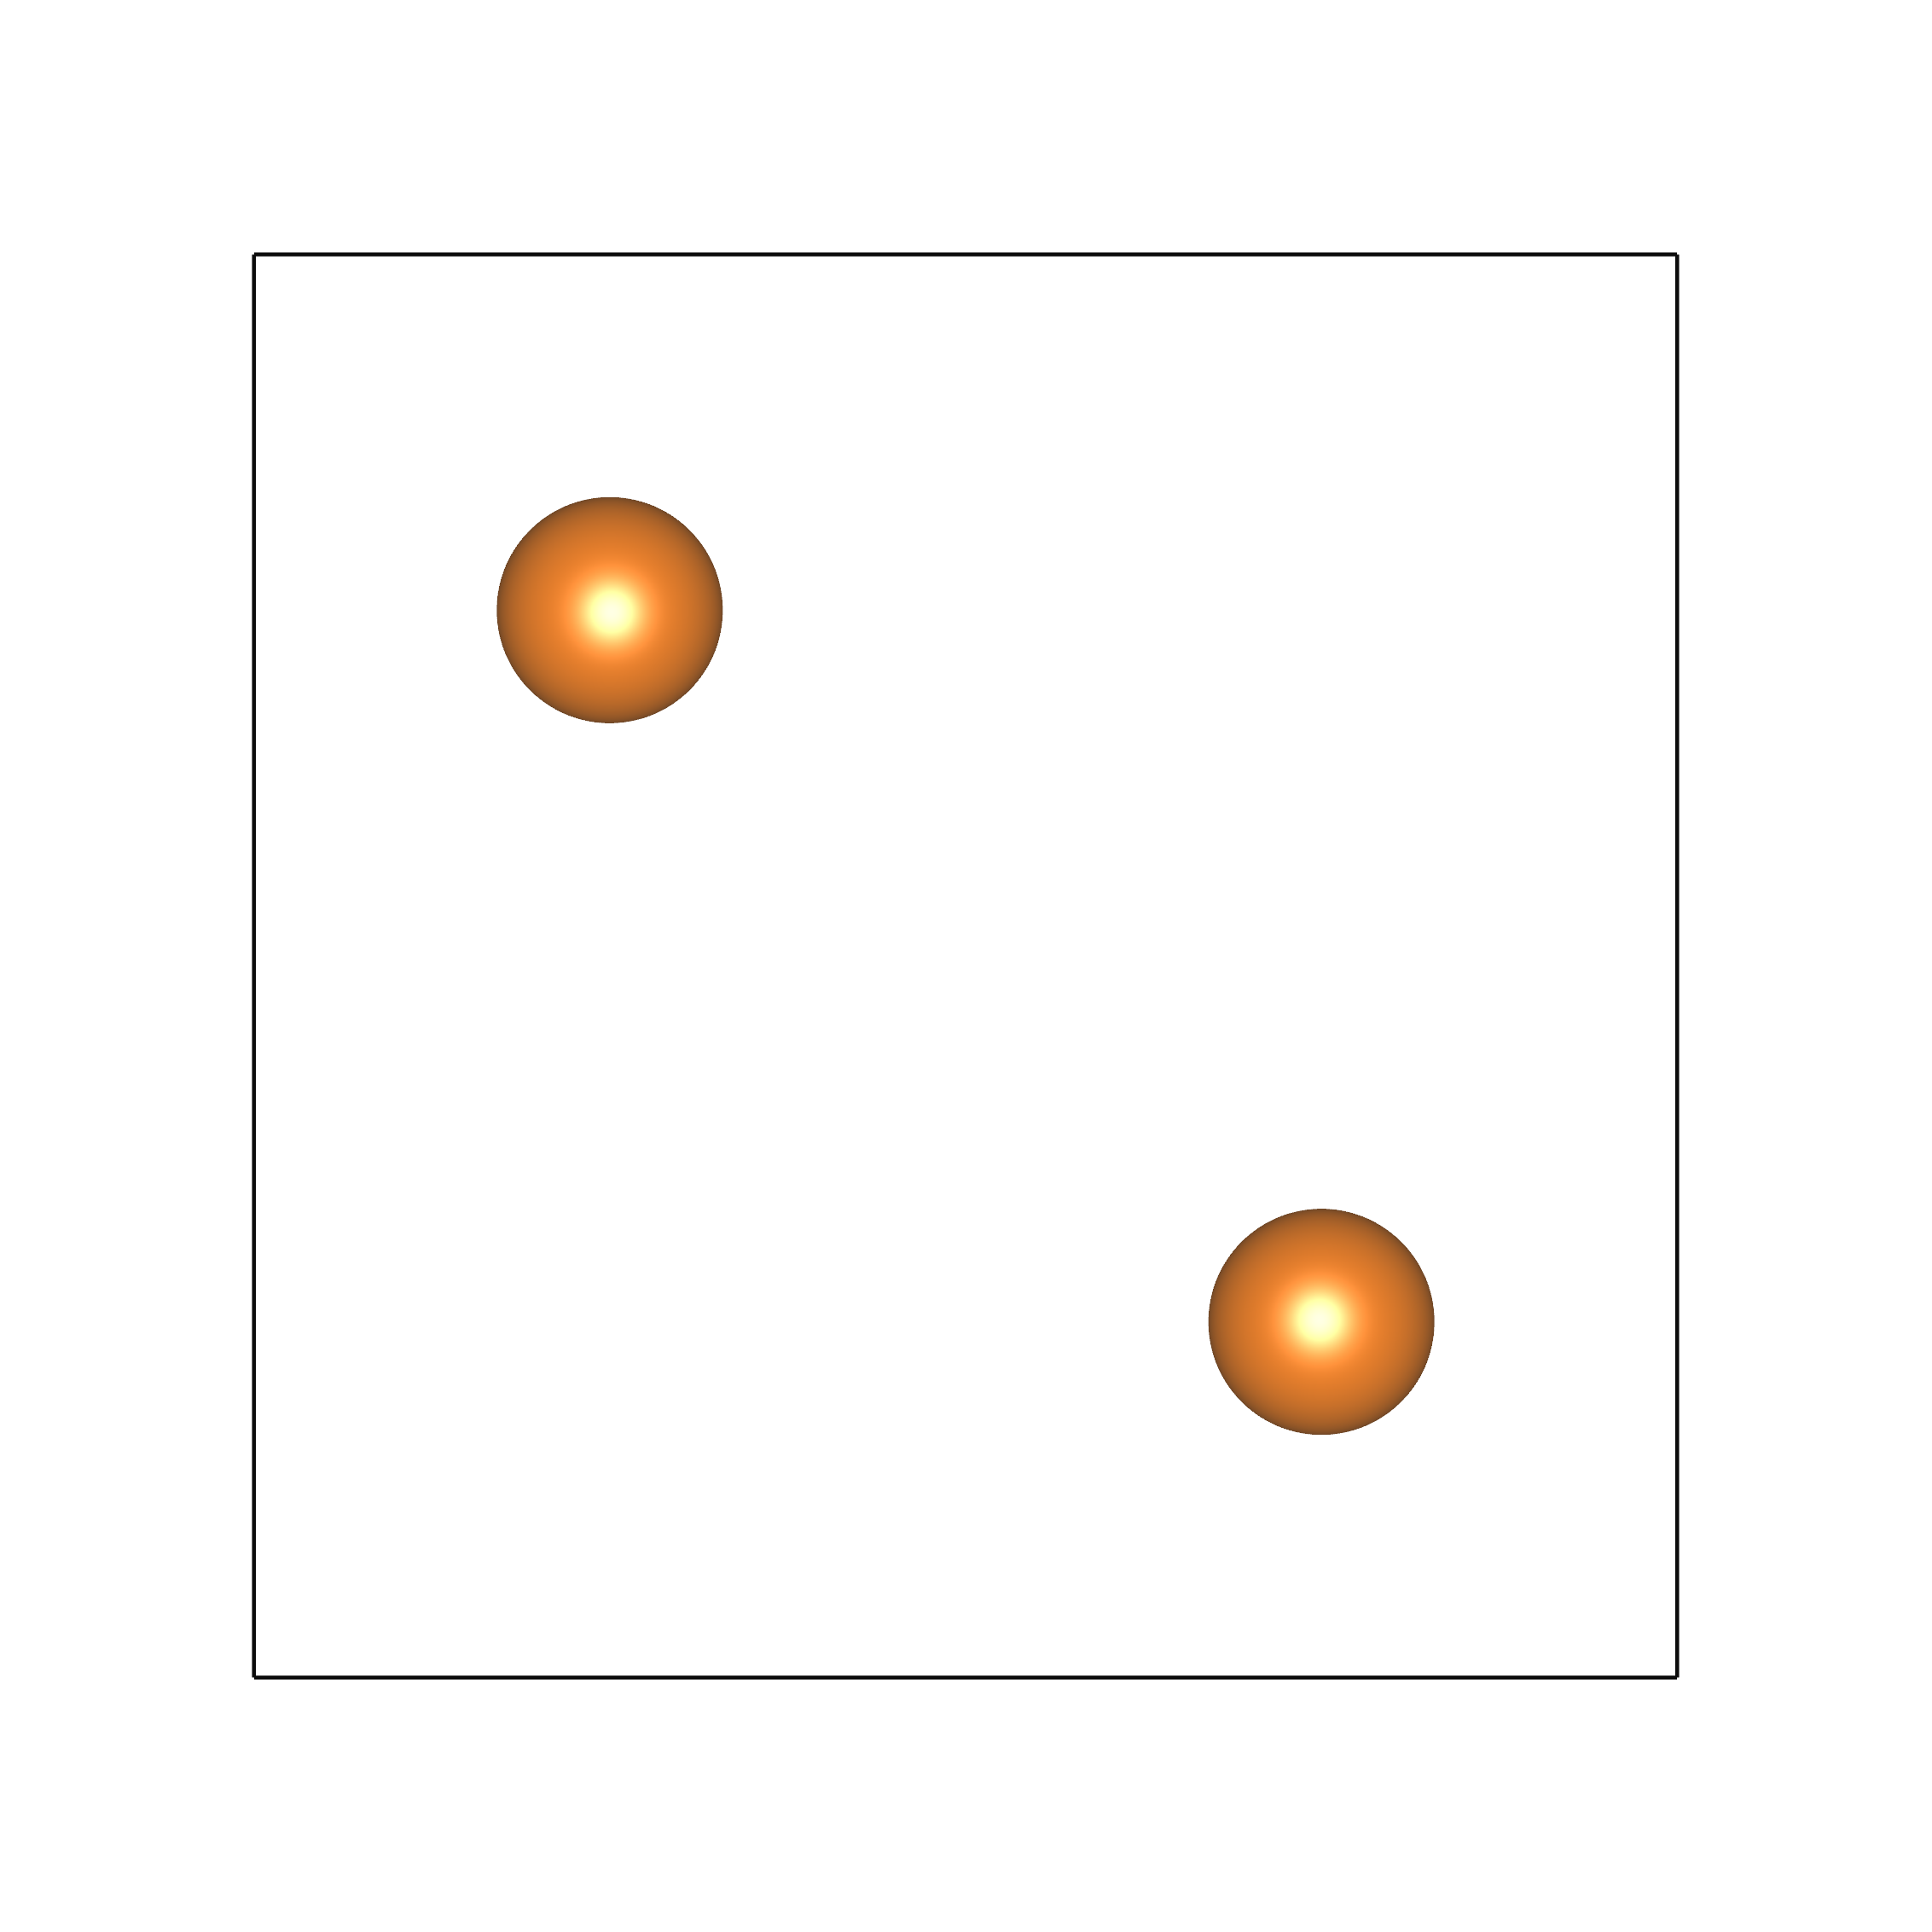
\includegraphics[scale=0.03]{Ch10/Spinel/spl6}
	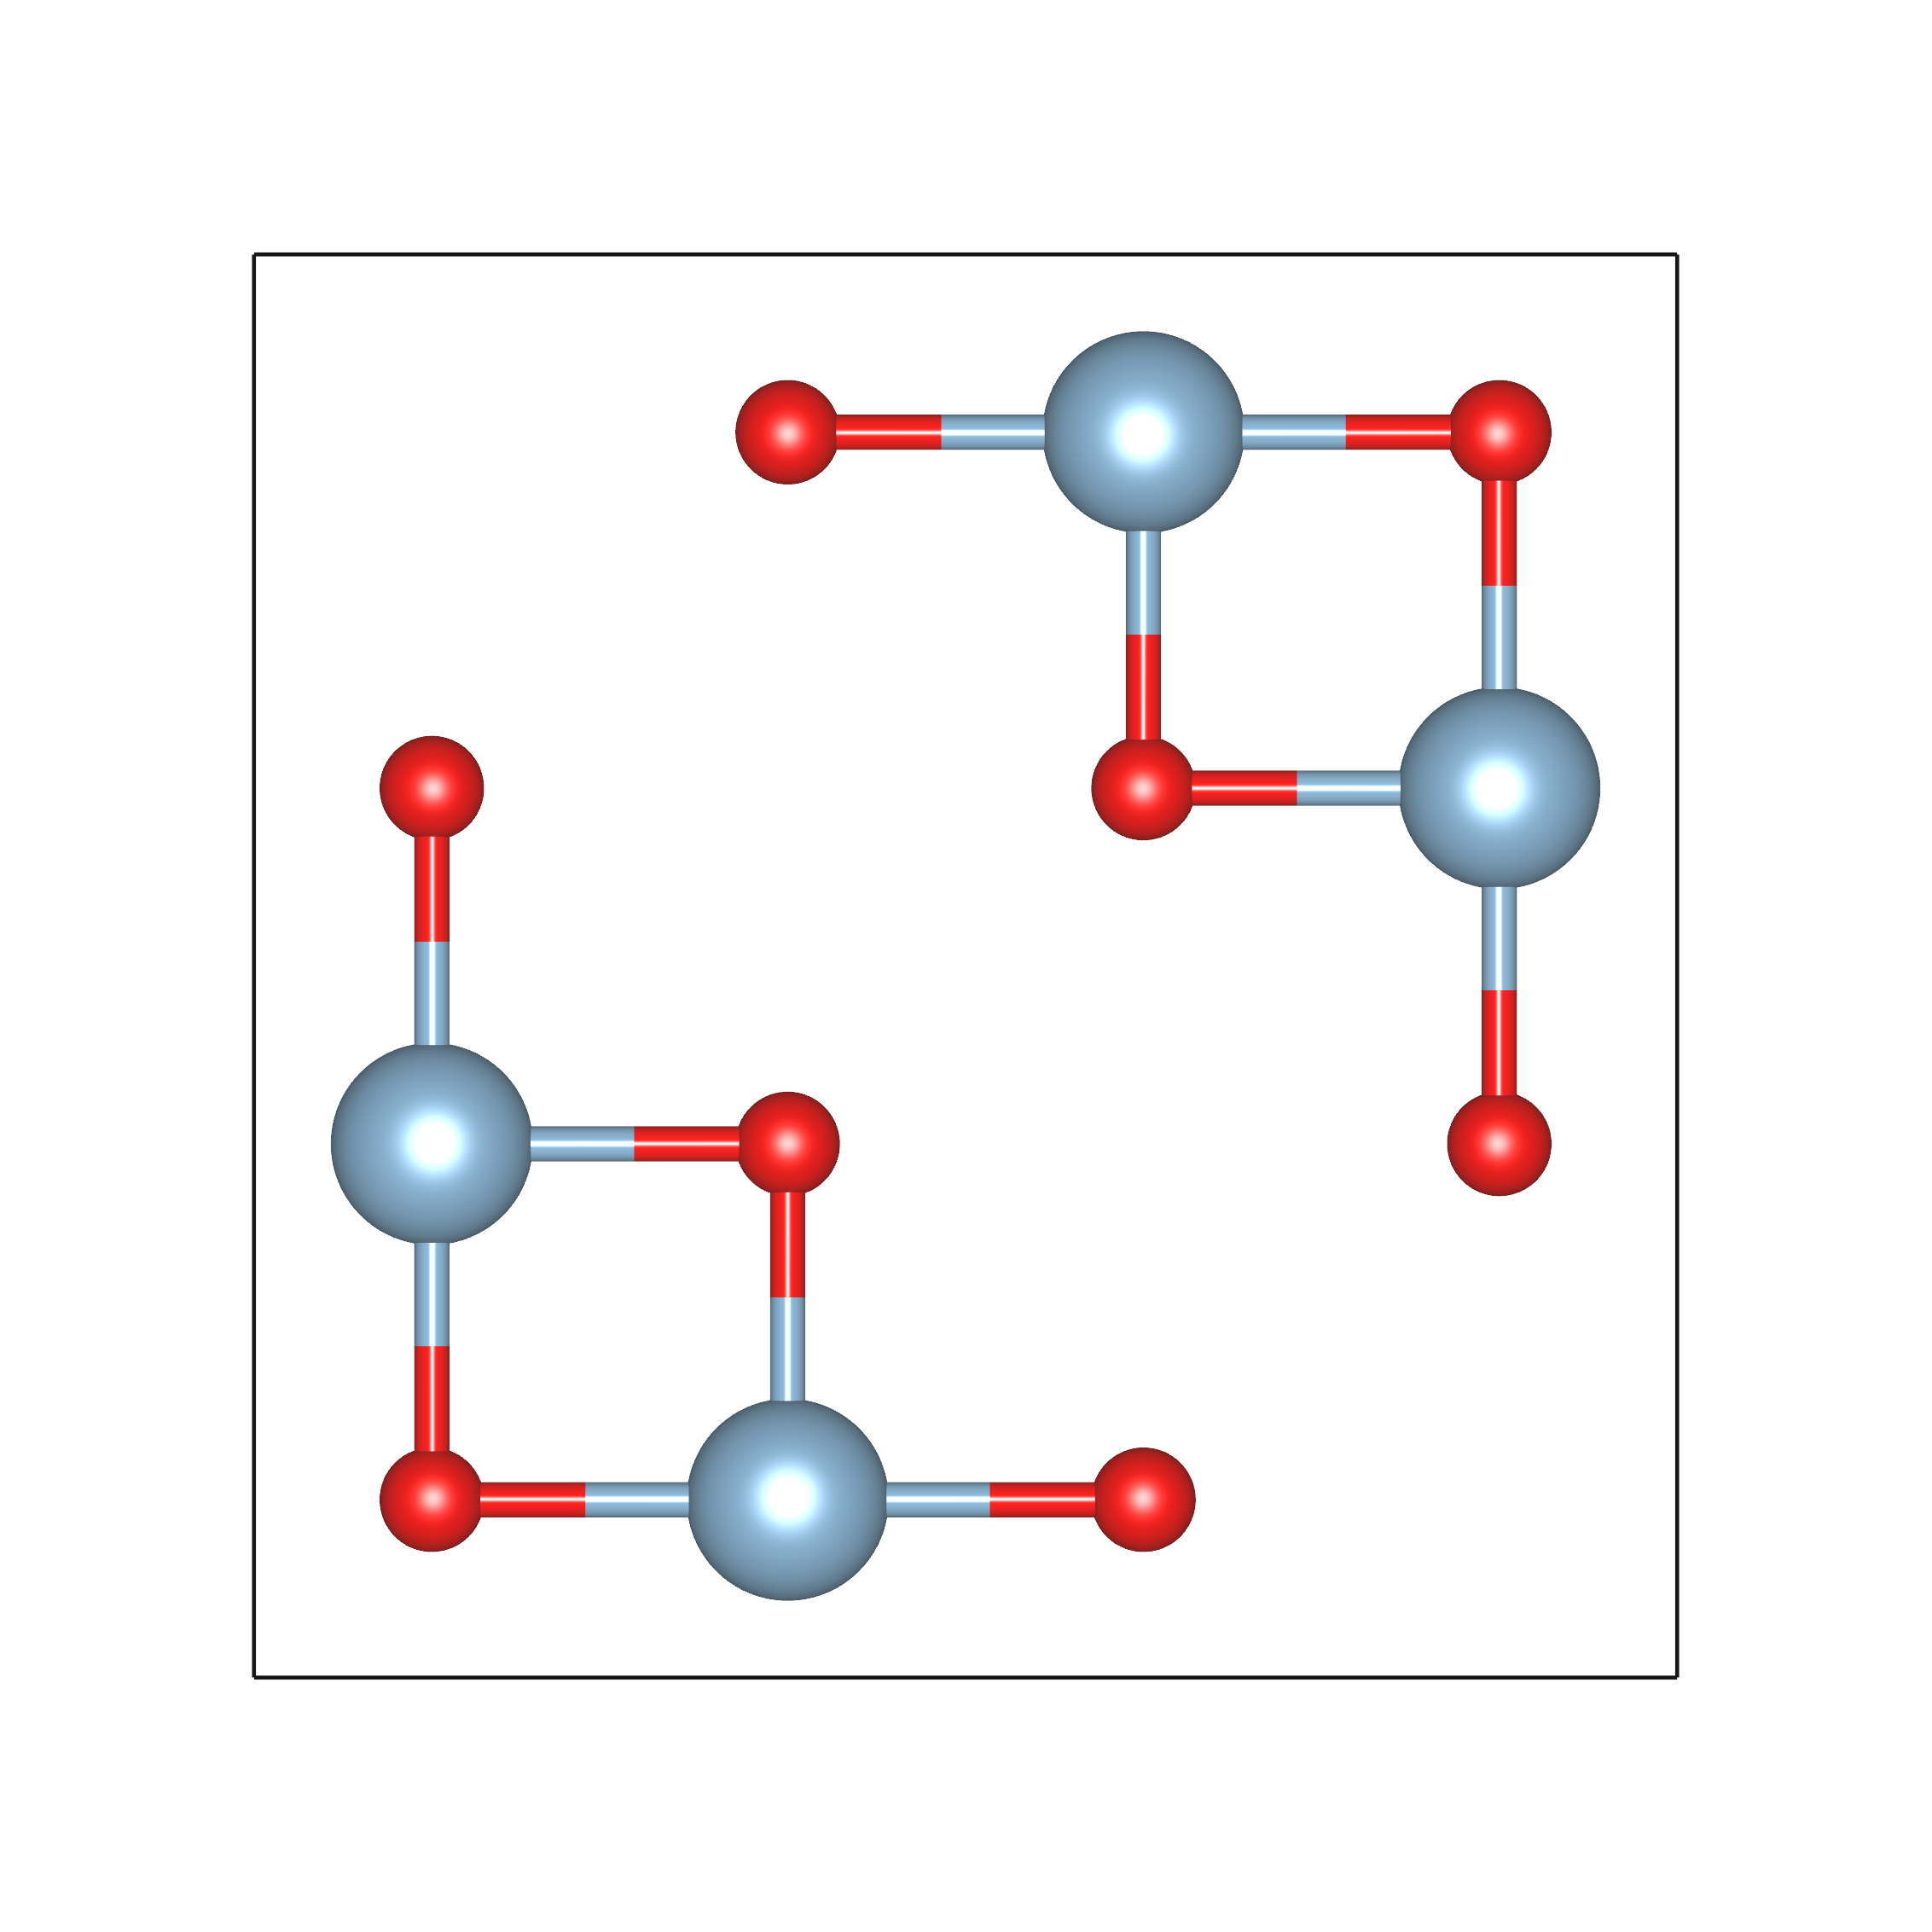
\includegraphics[scale=0.03]{Ch10/Spinel/spl7}
	\caption{Stacking of spinel from $c=0$ to 7/8}
	\label{spl}
\end{figure}\\
%
However there're inverse spinels where B occupy the tetrahedral sites where A once were and 
another 1/4 octahedral sites, and A take the rest 1/4 octahedral. 
This phenomenon can be explained by ligand field theory 
where the preference for coordination fields originates from LSFE (see \ref{preference}).\\ \\
Consider a spinel consists of $d^5$ and $d^6$ metals, as in $\rm Fe_3O_4$.
Since $d^5$ metals gain no LSFE from either tetrahedral or octahedral sites, 
it will leave the octahedral sites for $d^6$ metals which have strong preference for octahedral field, 
so that the total LSFE can be maximized, leading to the formation of inverse spinel.
%
\subsection{Rutiles}
%
At first glance of rutile structure, where's the 4-fold axis? \\ \\
The structure can be described as strands of $\rm [TiO_6]$ octahedra extending along $c$. 
Within each strand the octahedra are connected by shared opposite edges. 
There're two groups of strands which differ by a $c/2$ translation and a $90^{\circ}$ rotation. 
Shared vertices connect strands of different groups.
Rotating one strand $90^{\circ}$ and then translate by $c/2$ gives the other strand.
And voila, this gives the $4_2$ screw axis, as shown in figure \ref{rutile}.\\
%
\begin{figure}[h]
	\centering
	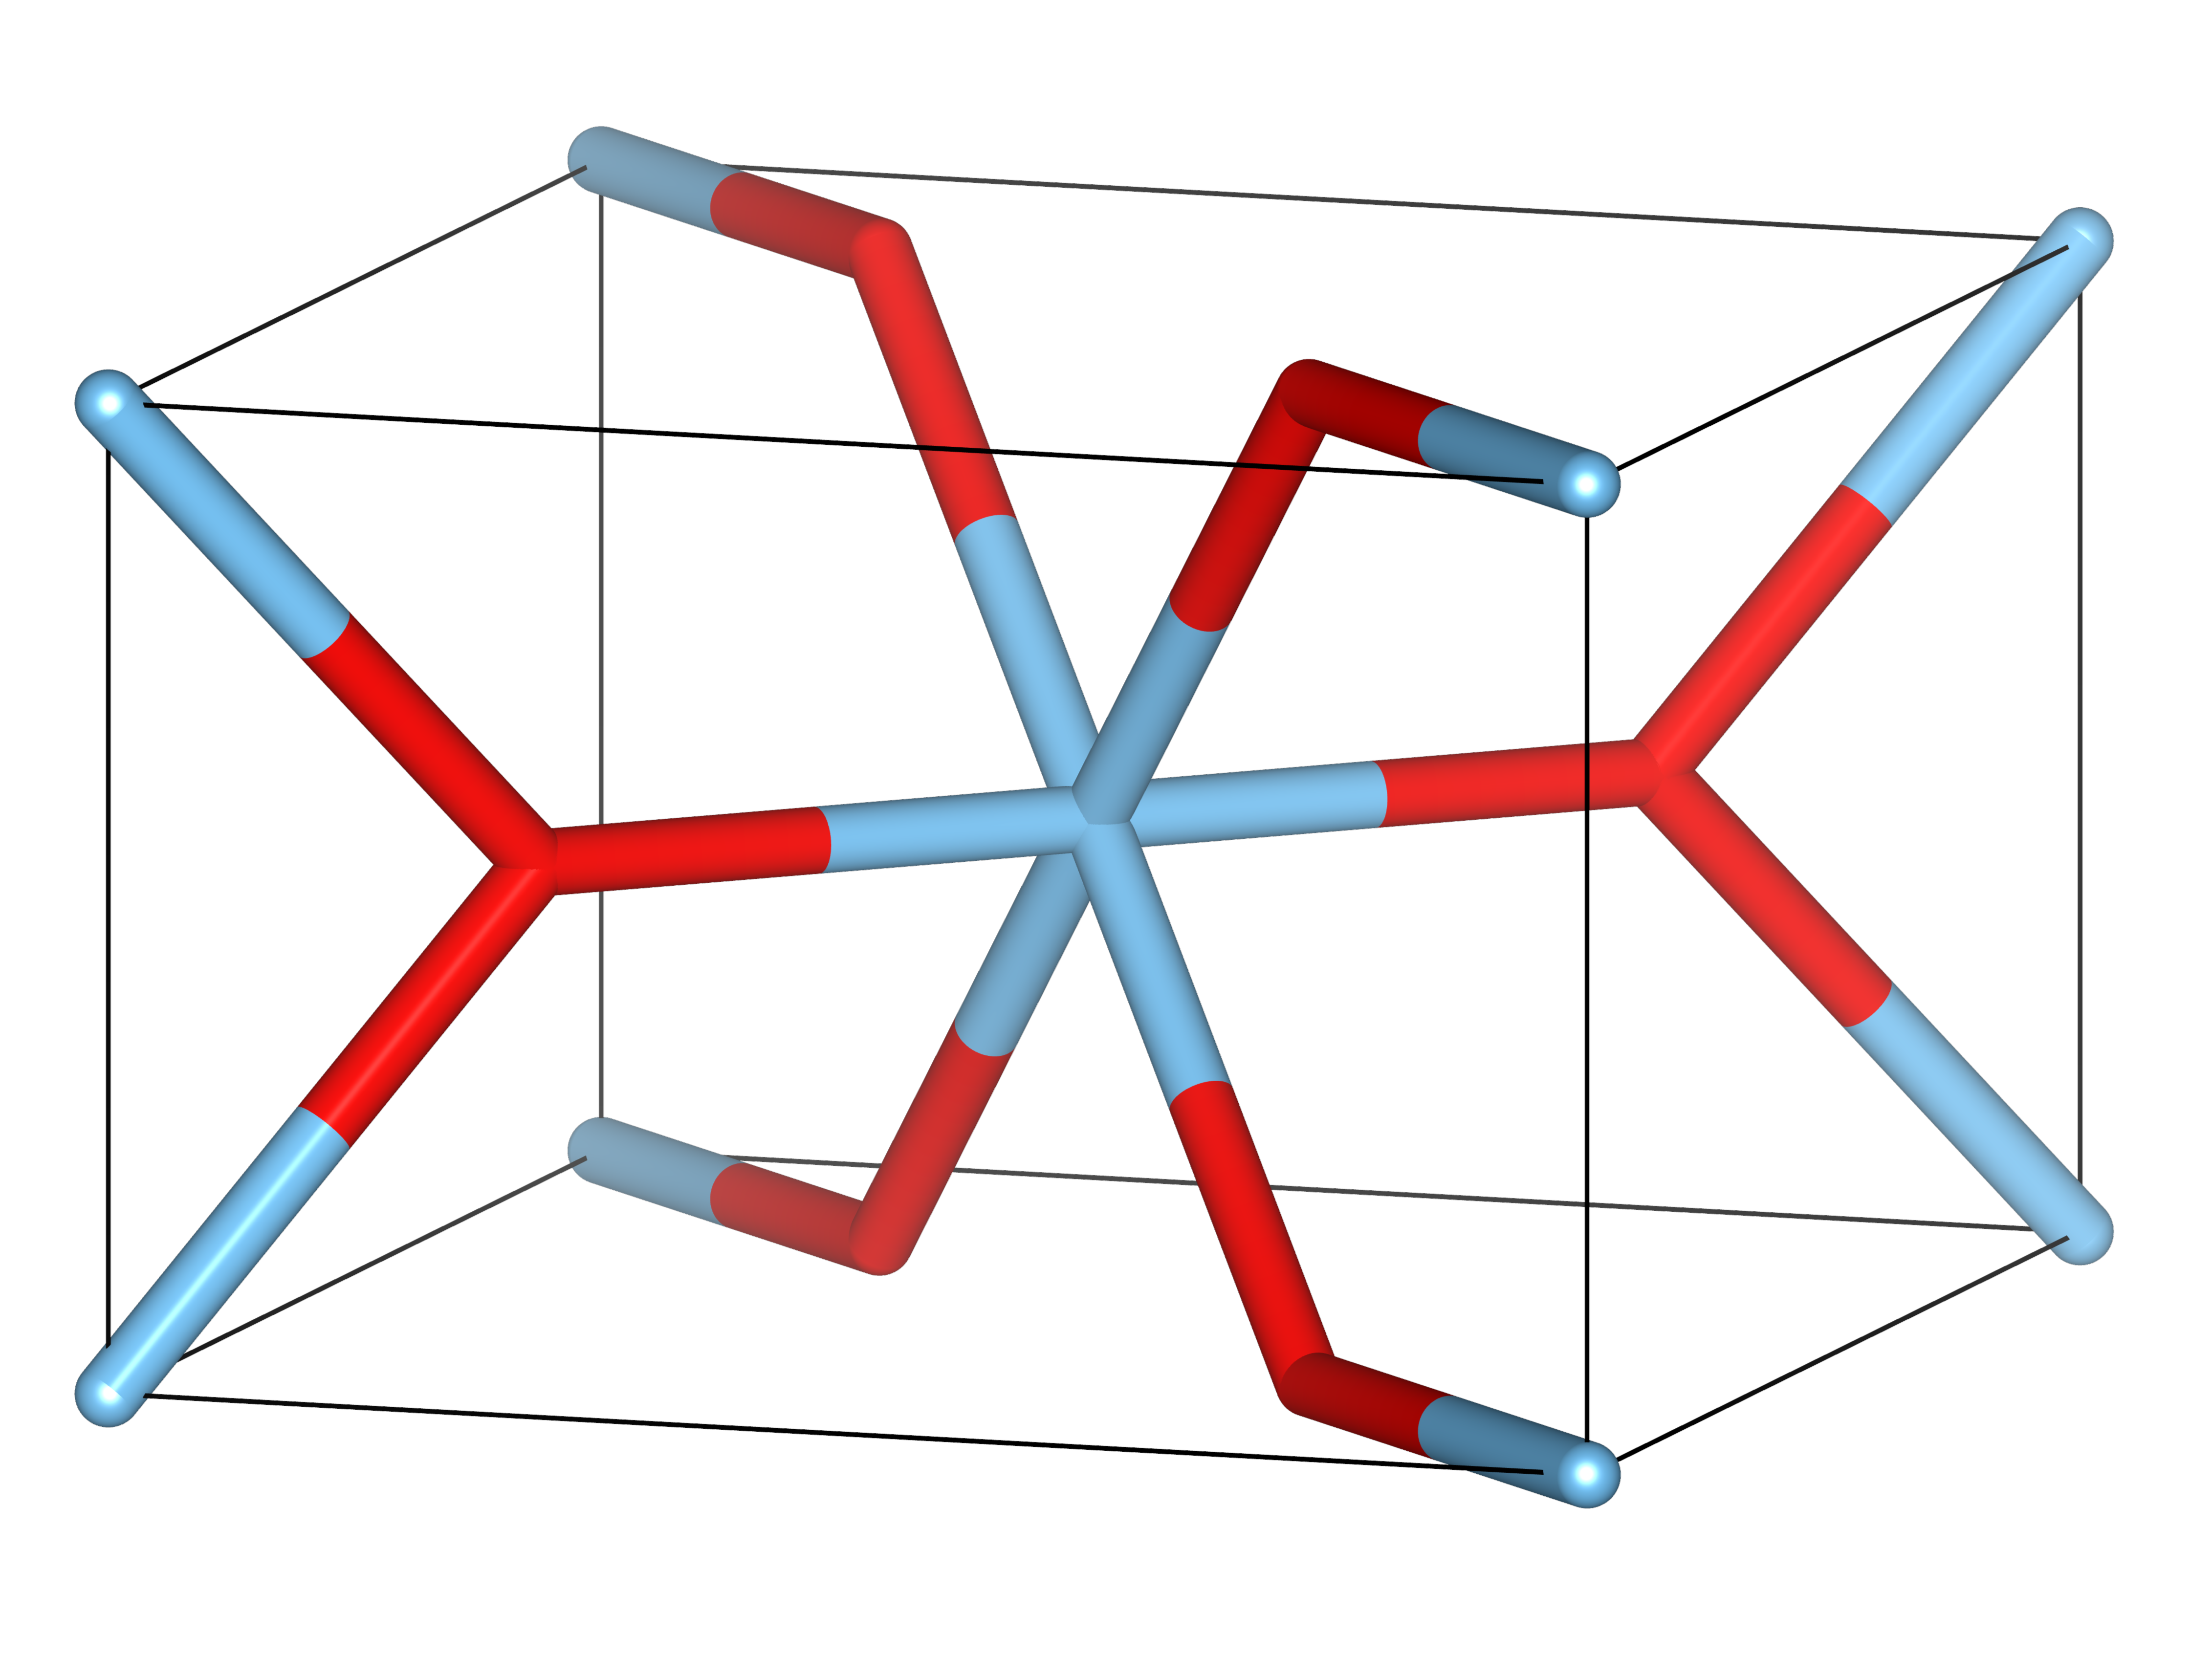
\includegraphics[scale=0.04]{Ch10/Rutile/rutile}
	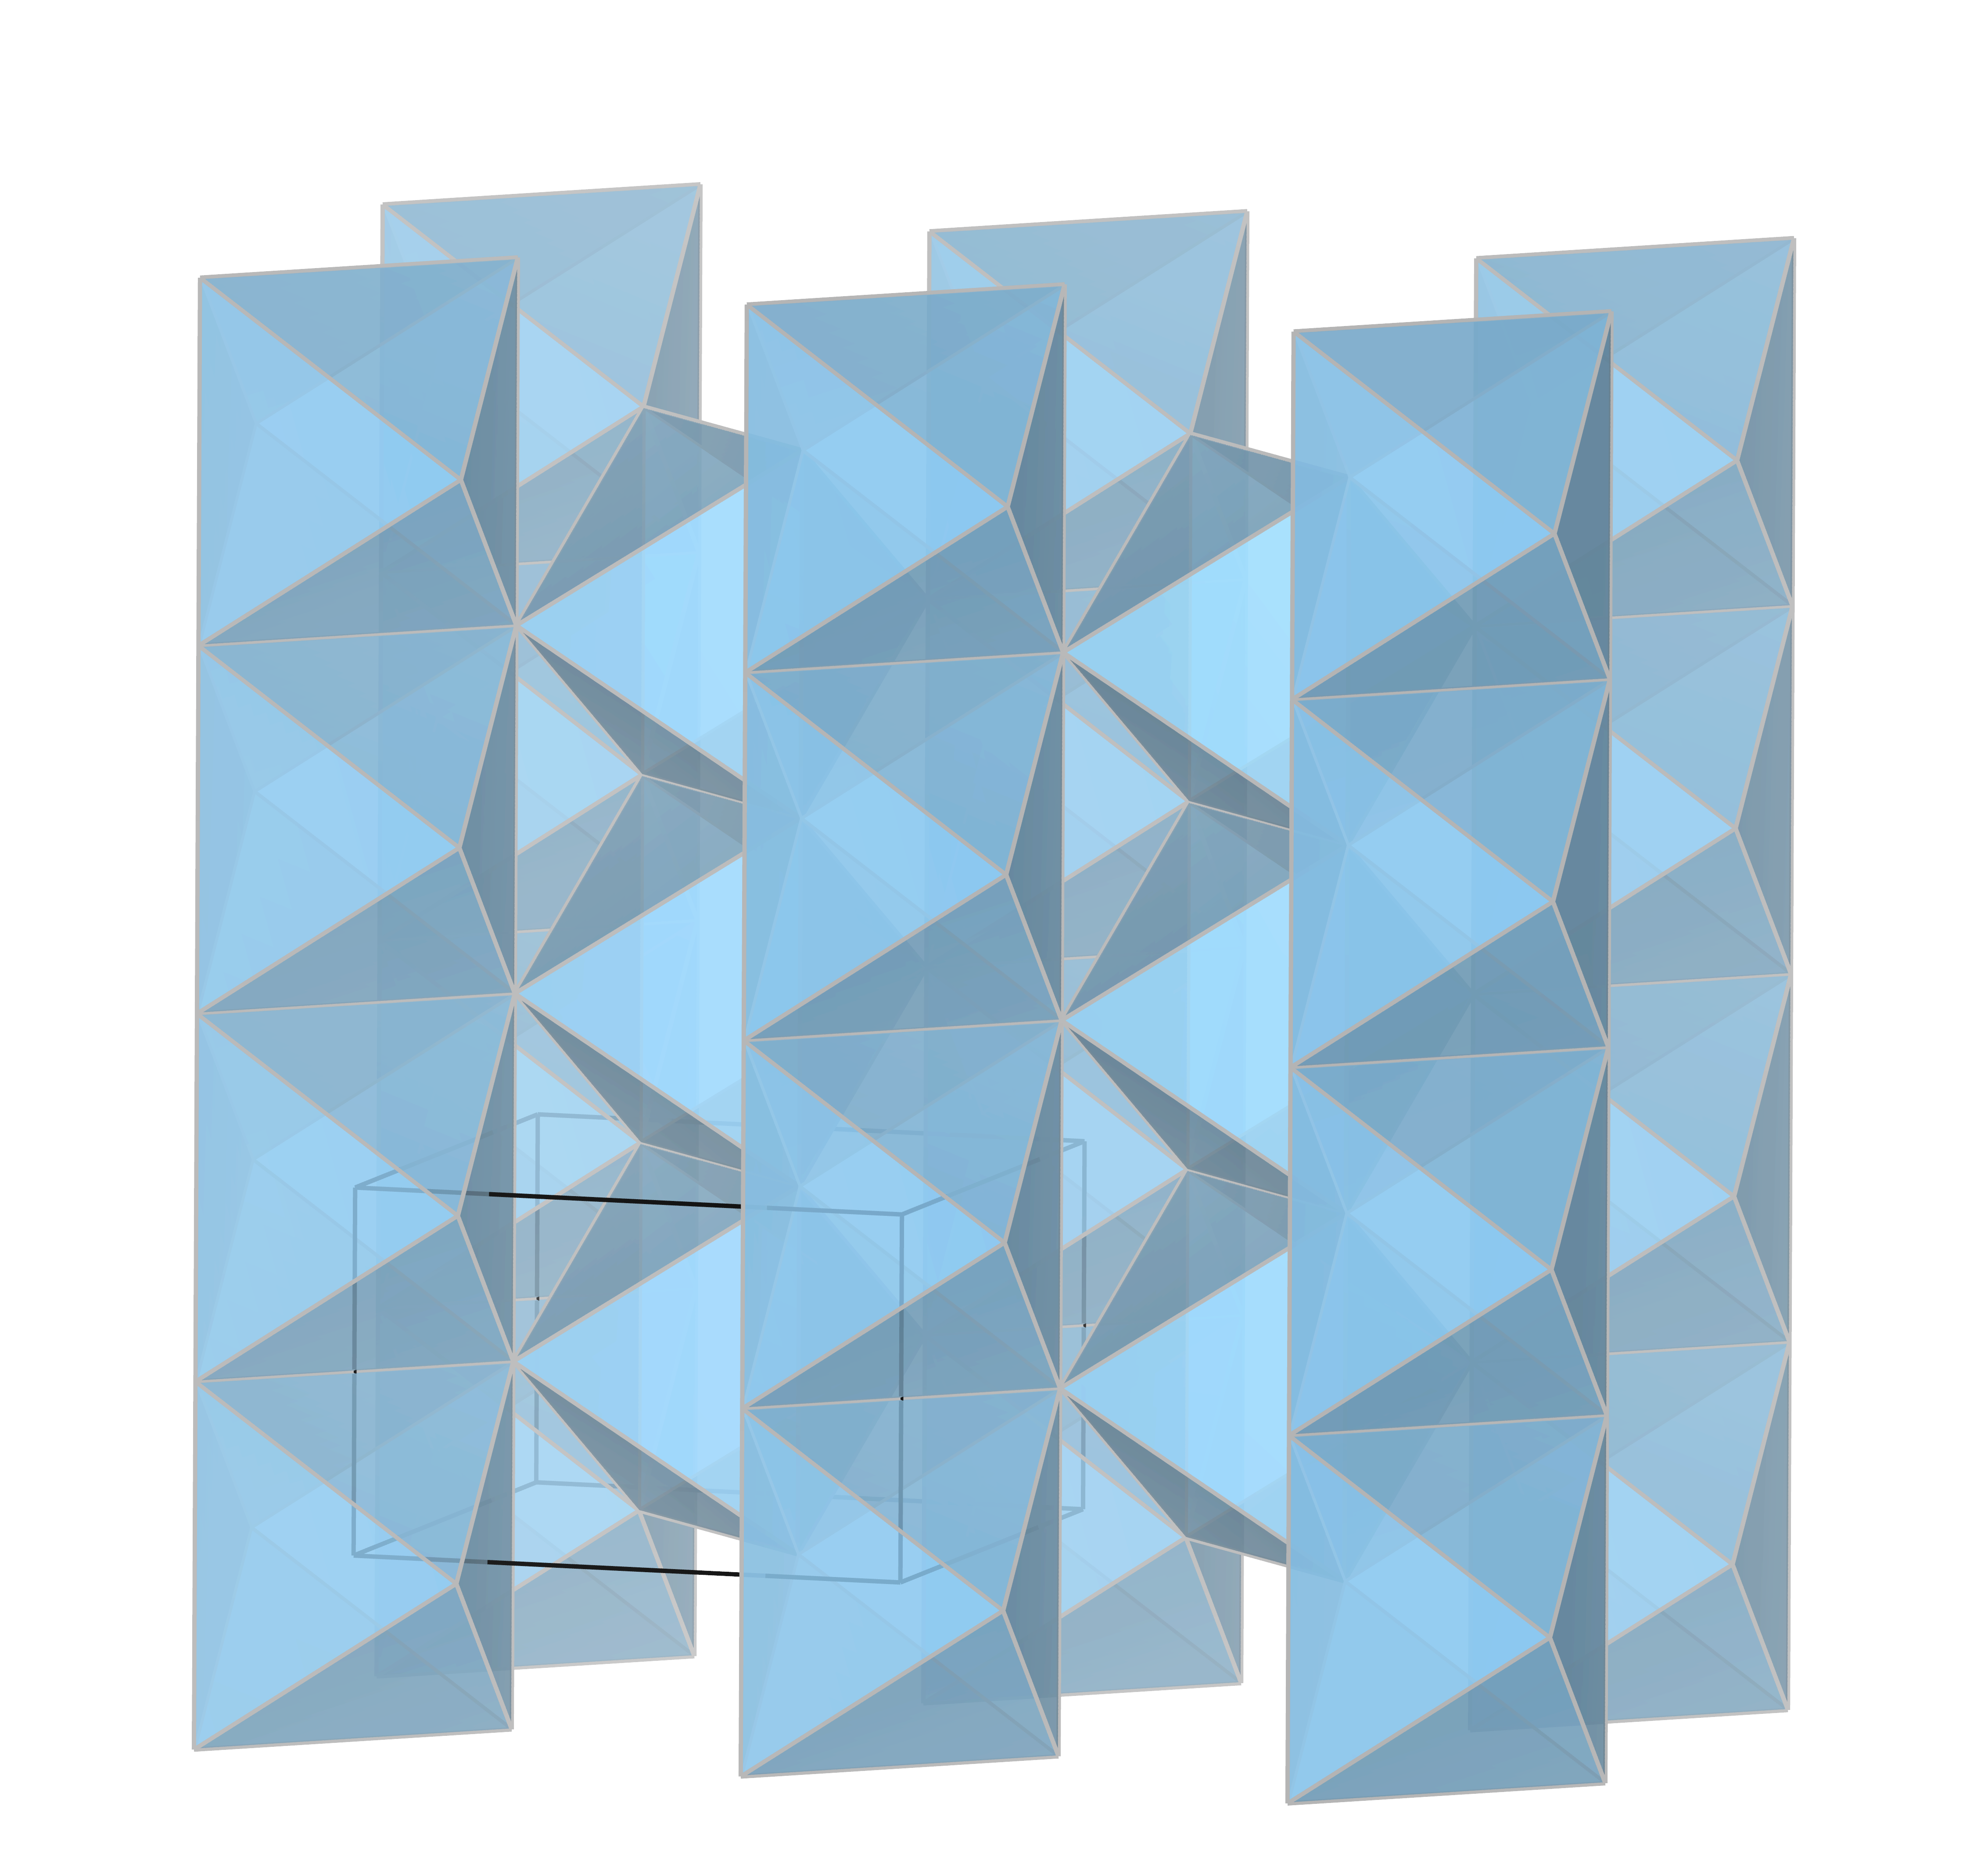
\includegraphics[scale=0.04]{Ch10/Rutile/rutile_strand}
	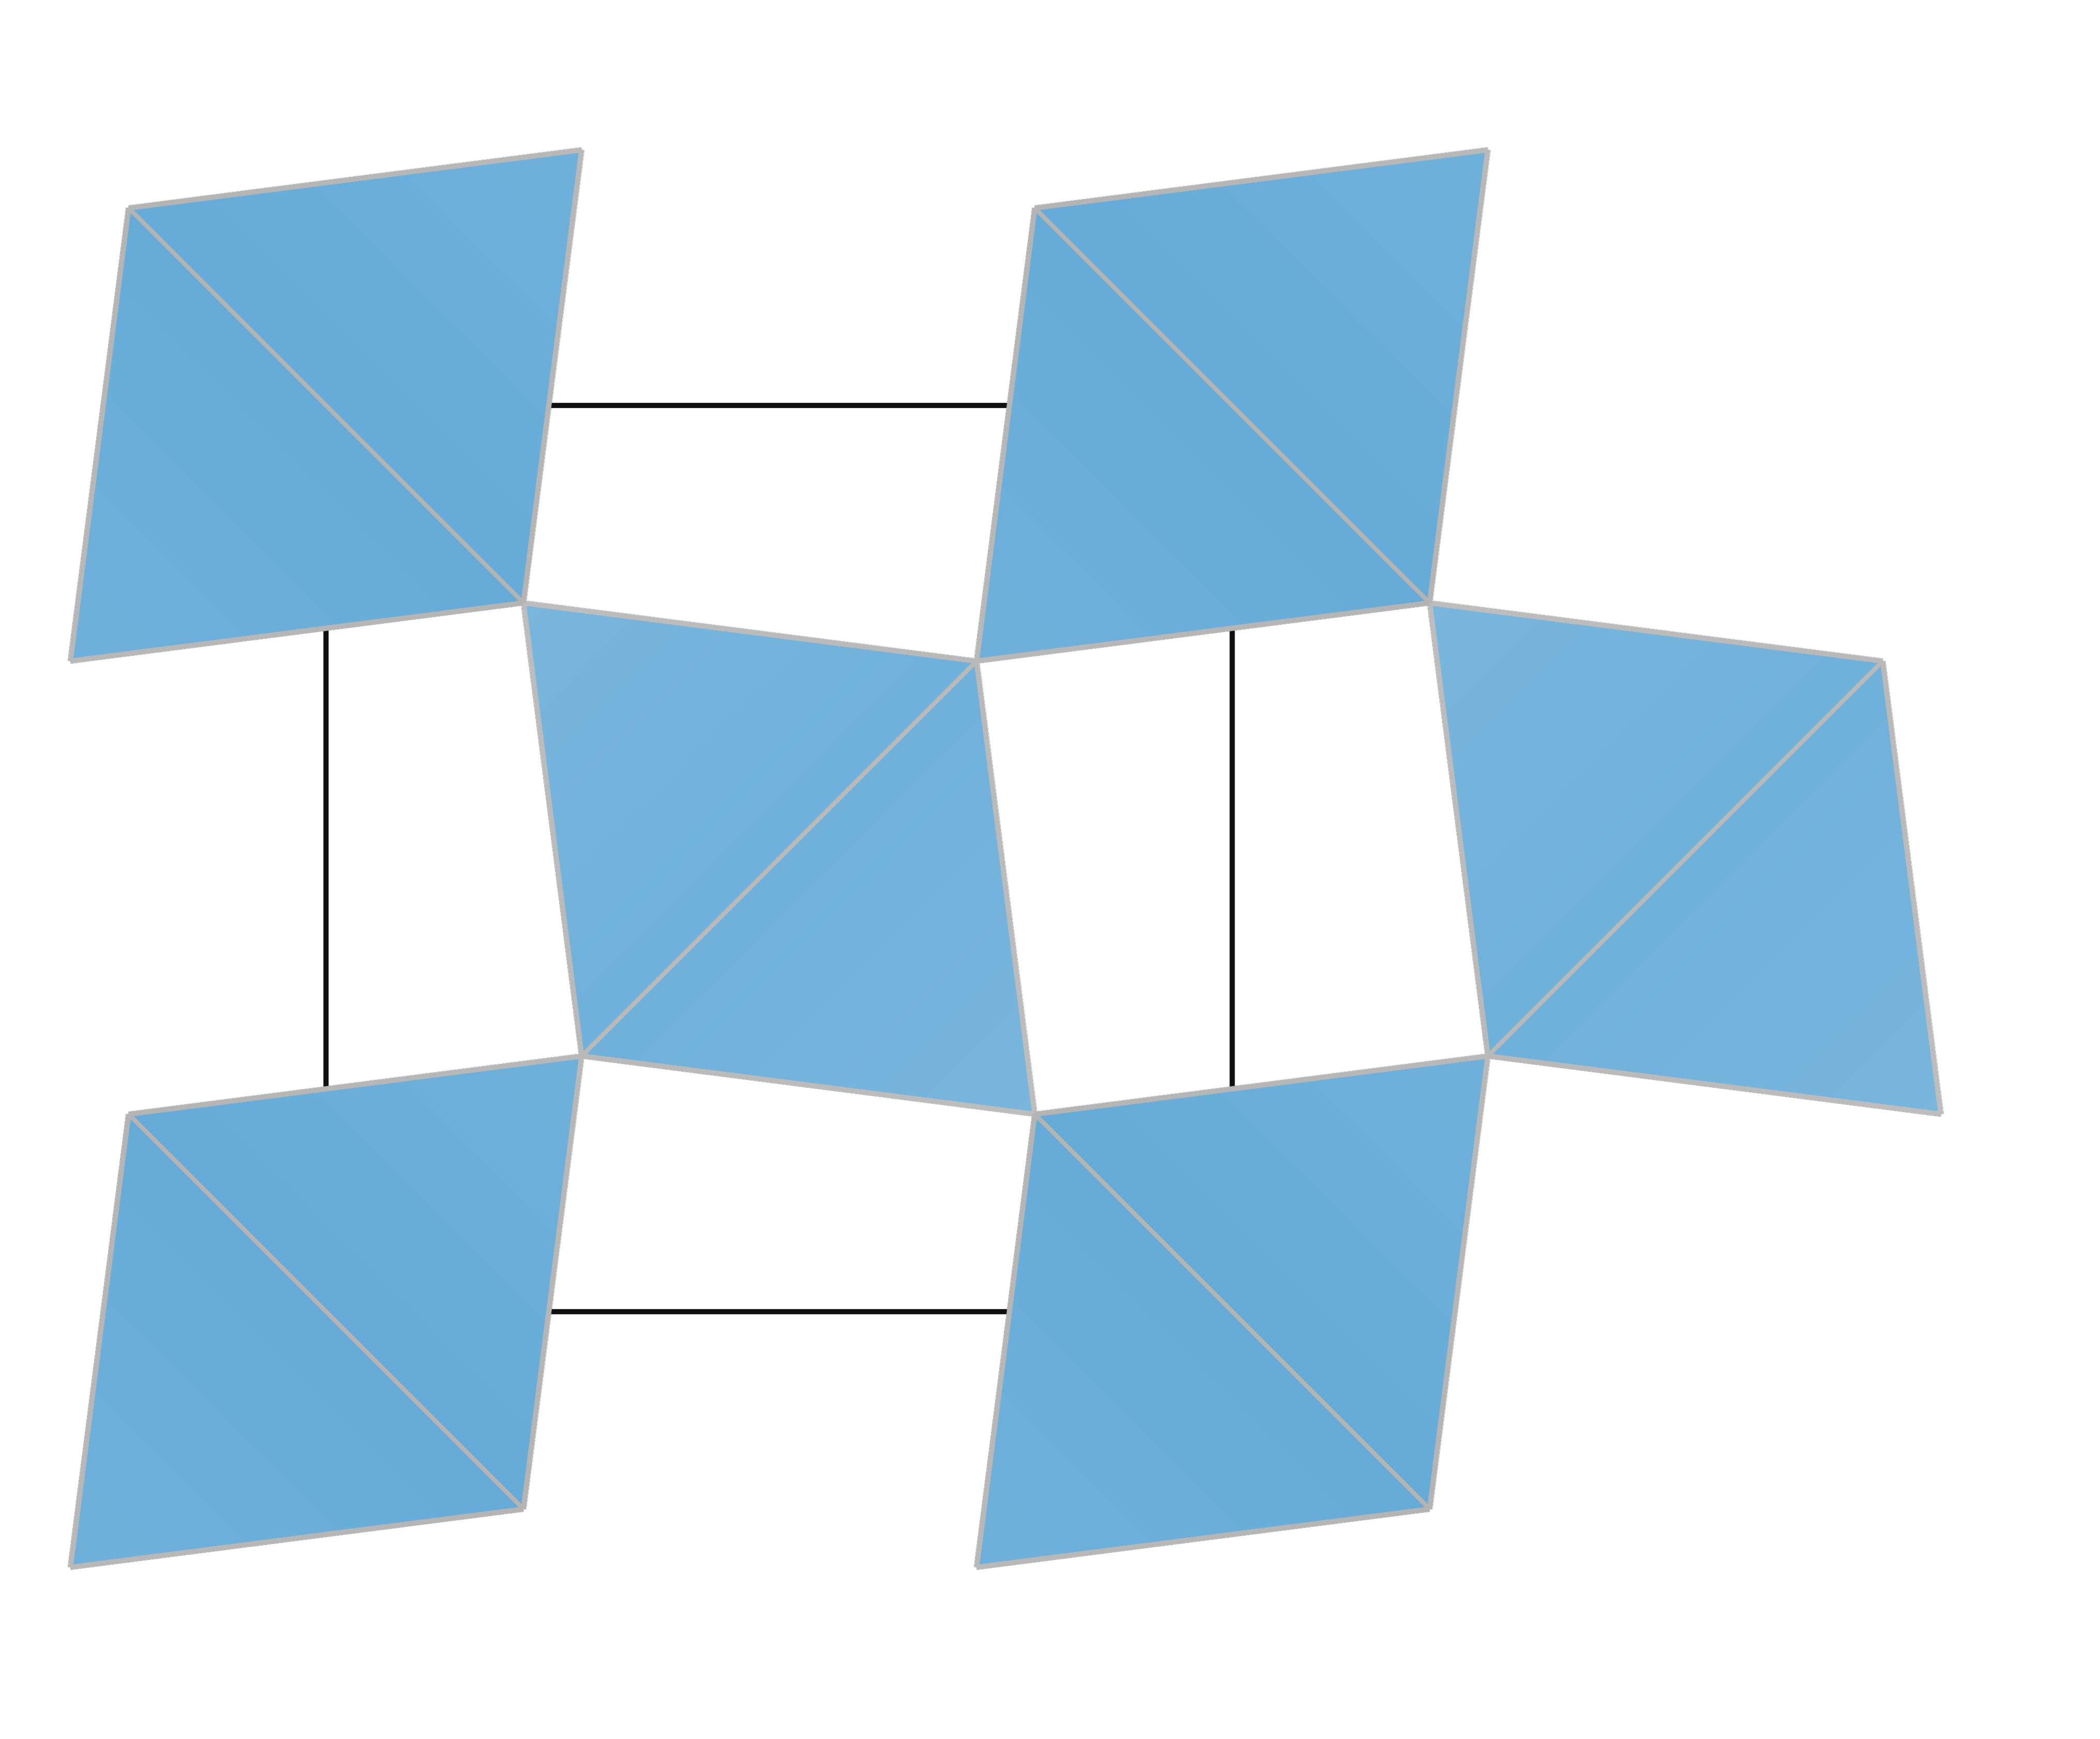
\includegraphics[scale=0.04]{Ch10/Rutile/rutile42}
	\caption{Rutile strand structure and $4_2$ screw axis.}
	\label{rutile}
\end{figure}\\
%
Other structures that can be similarly described as strands whose projections have only 2-fold axes 
may also adopt rutile structure.
Take $\rm NbOCl_3$ as an example, the structure motif for each strand is two $\rm [NbCl_4O_2]$ octahedra with a shared $\rm 2Cl$ edge.
Its structure is shown in figure \ref{nbocl3}.\\
%
\begin{figure}[h]
	\centering
	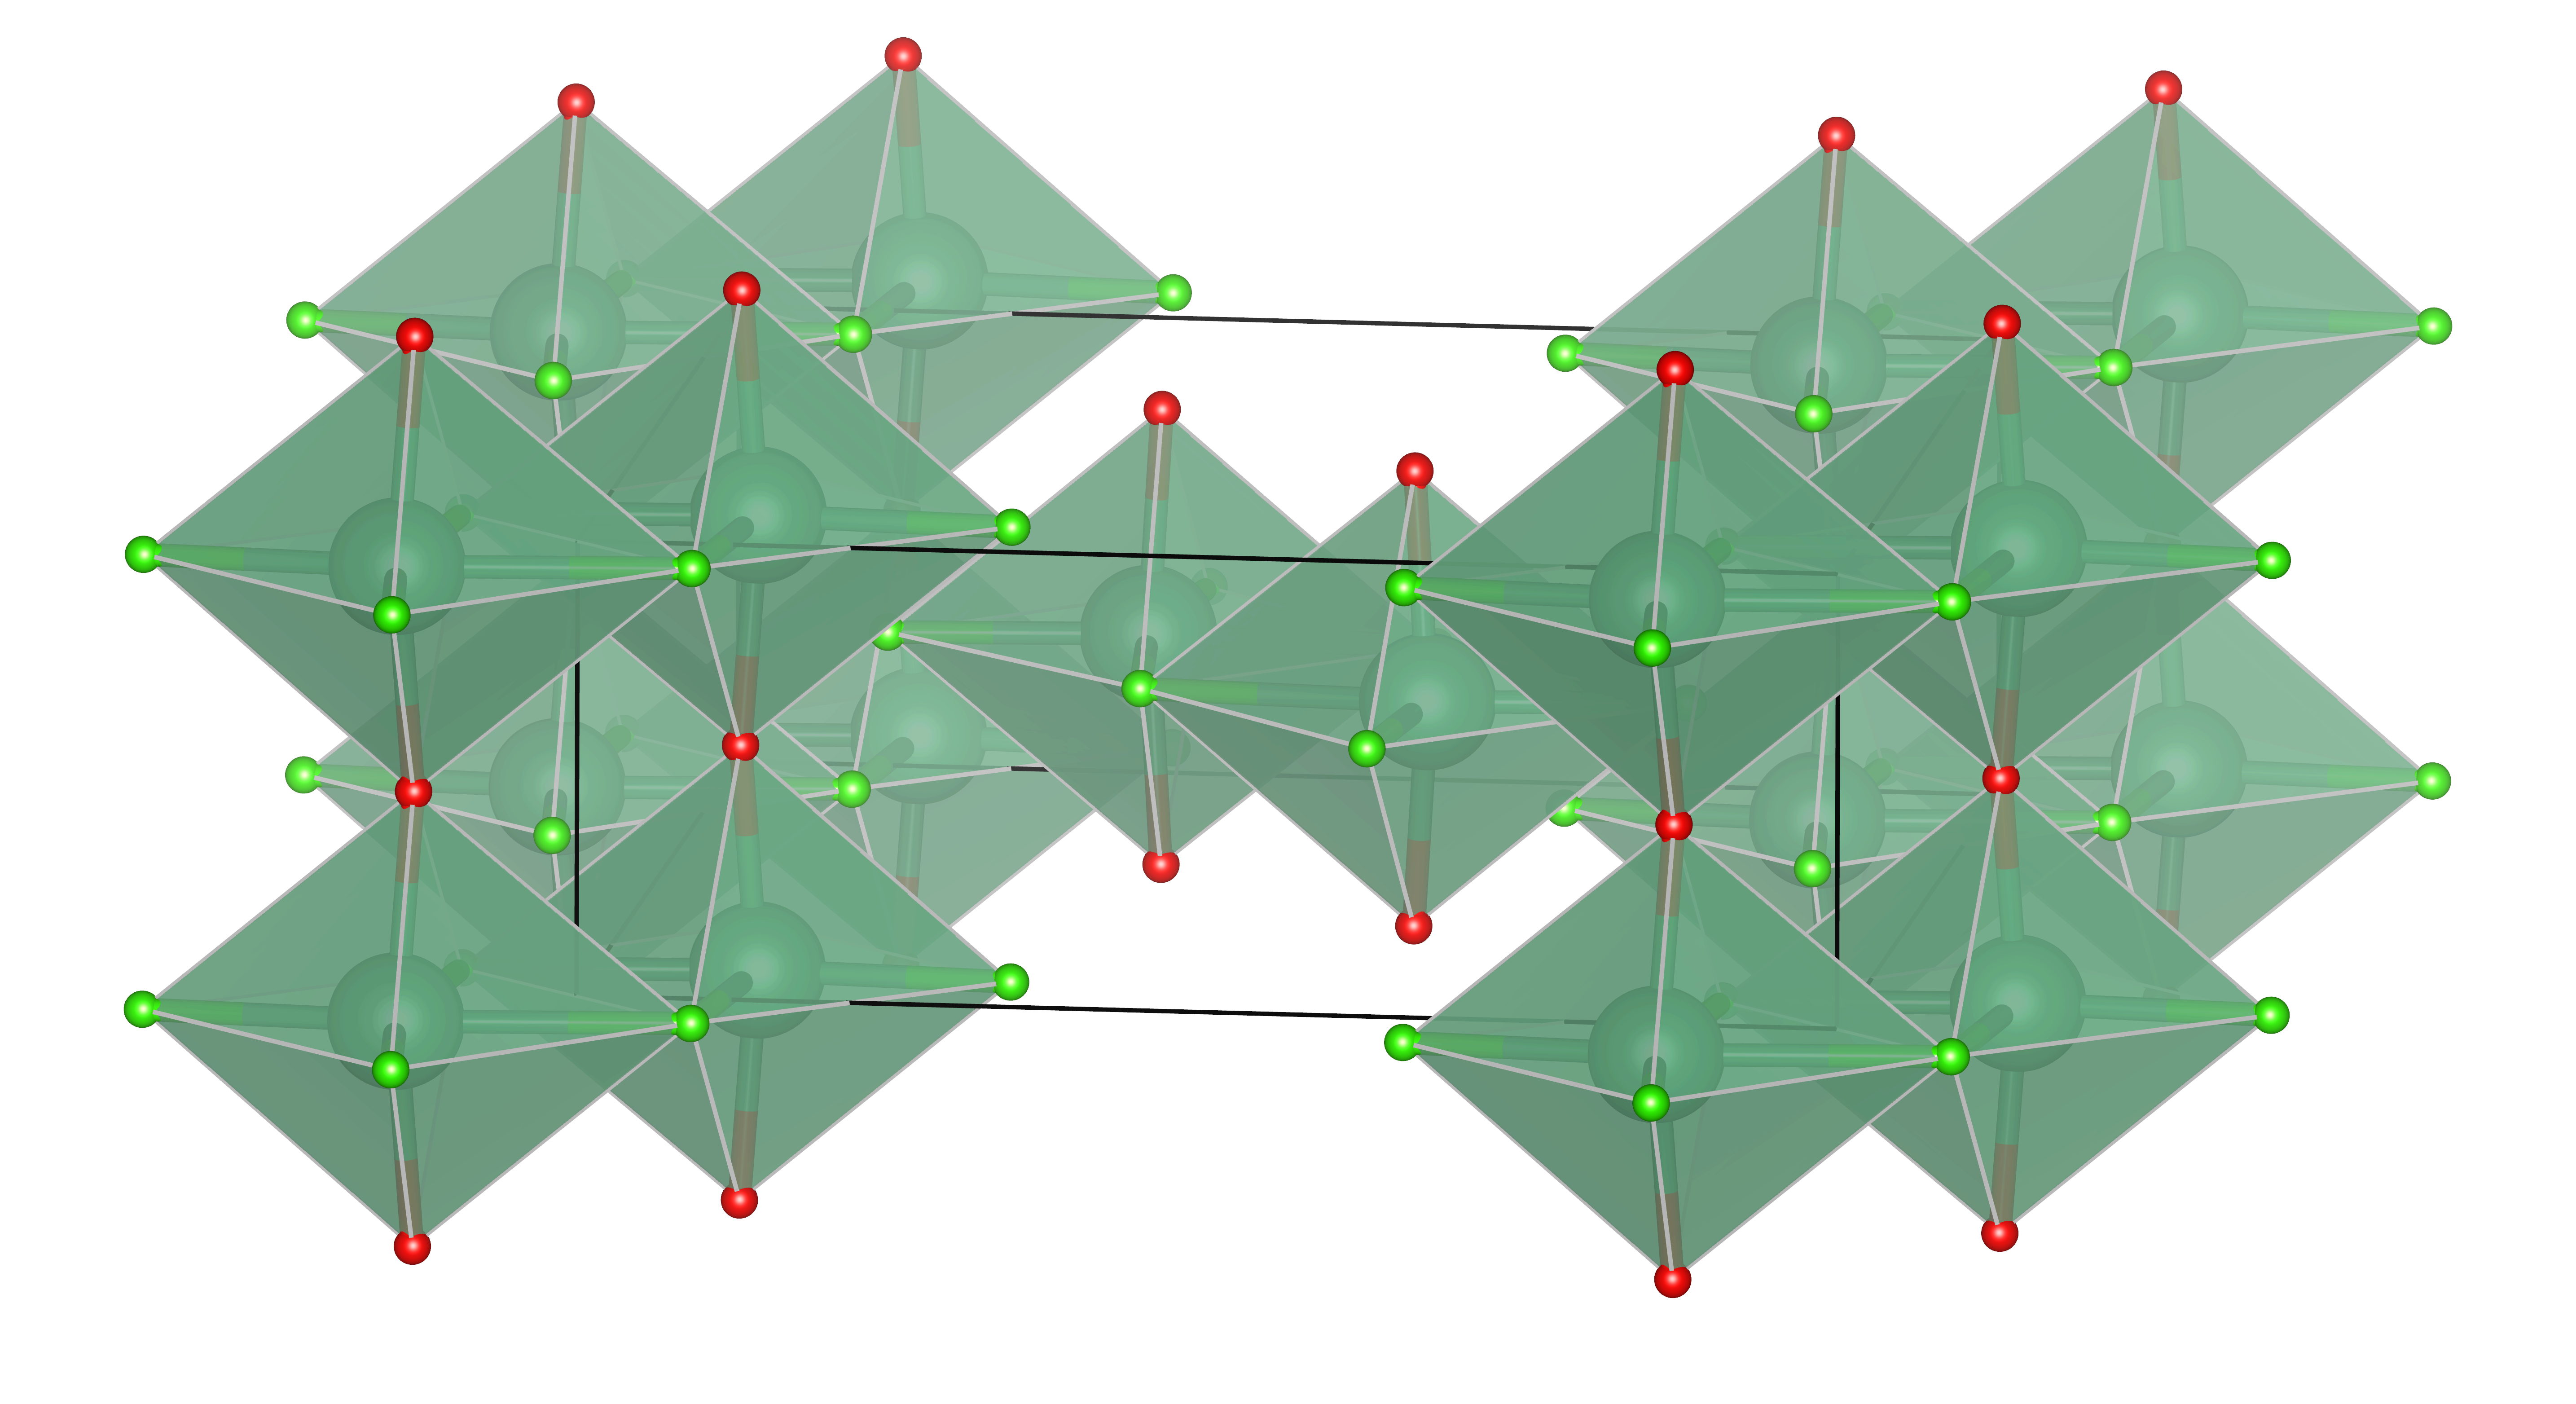
\includegraphics[scale=0.05]{Ch10/Rutile/NbOCl3_2}
	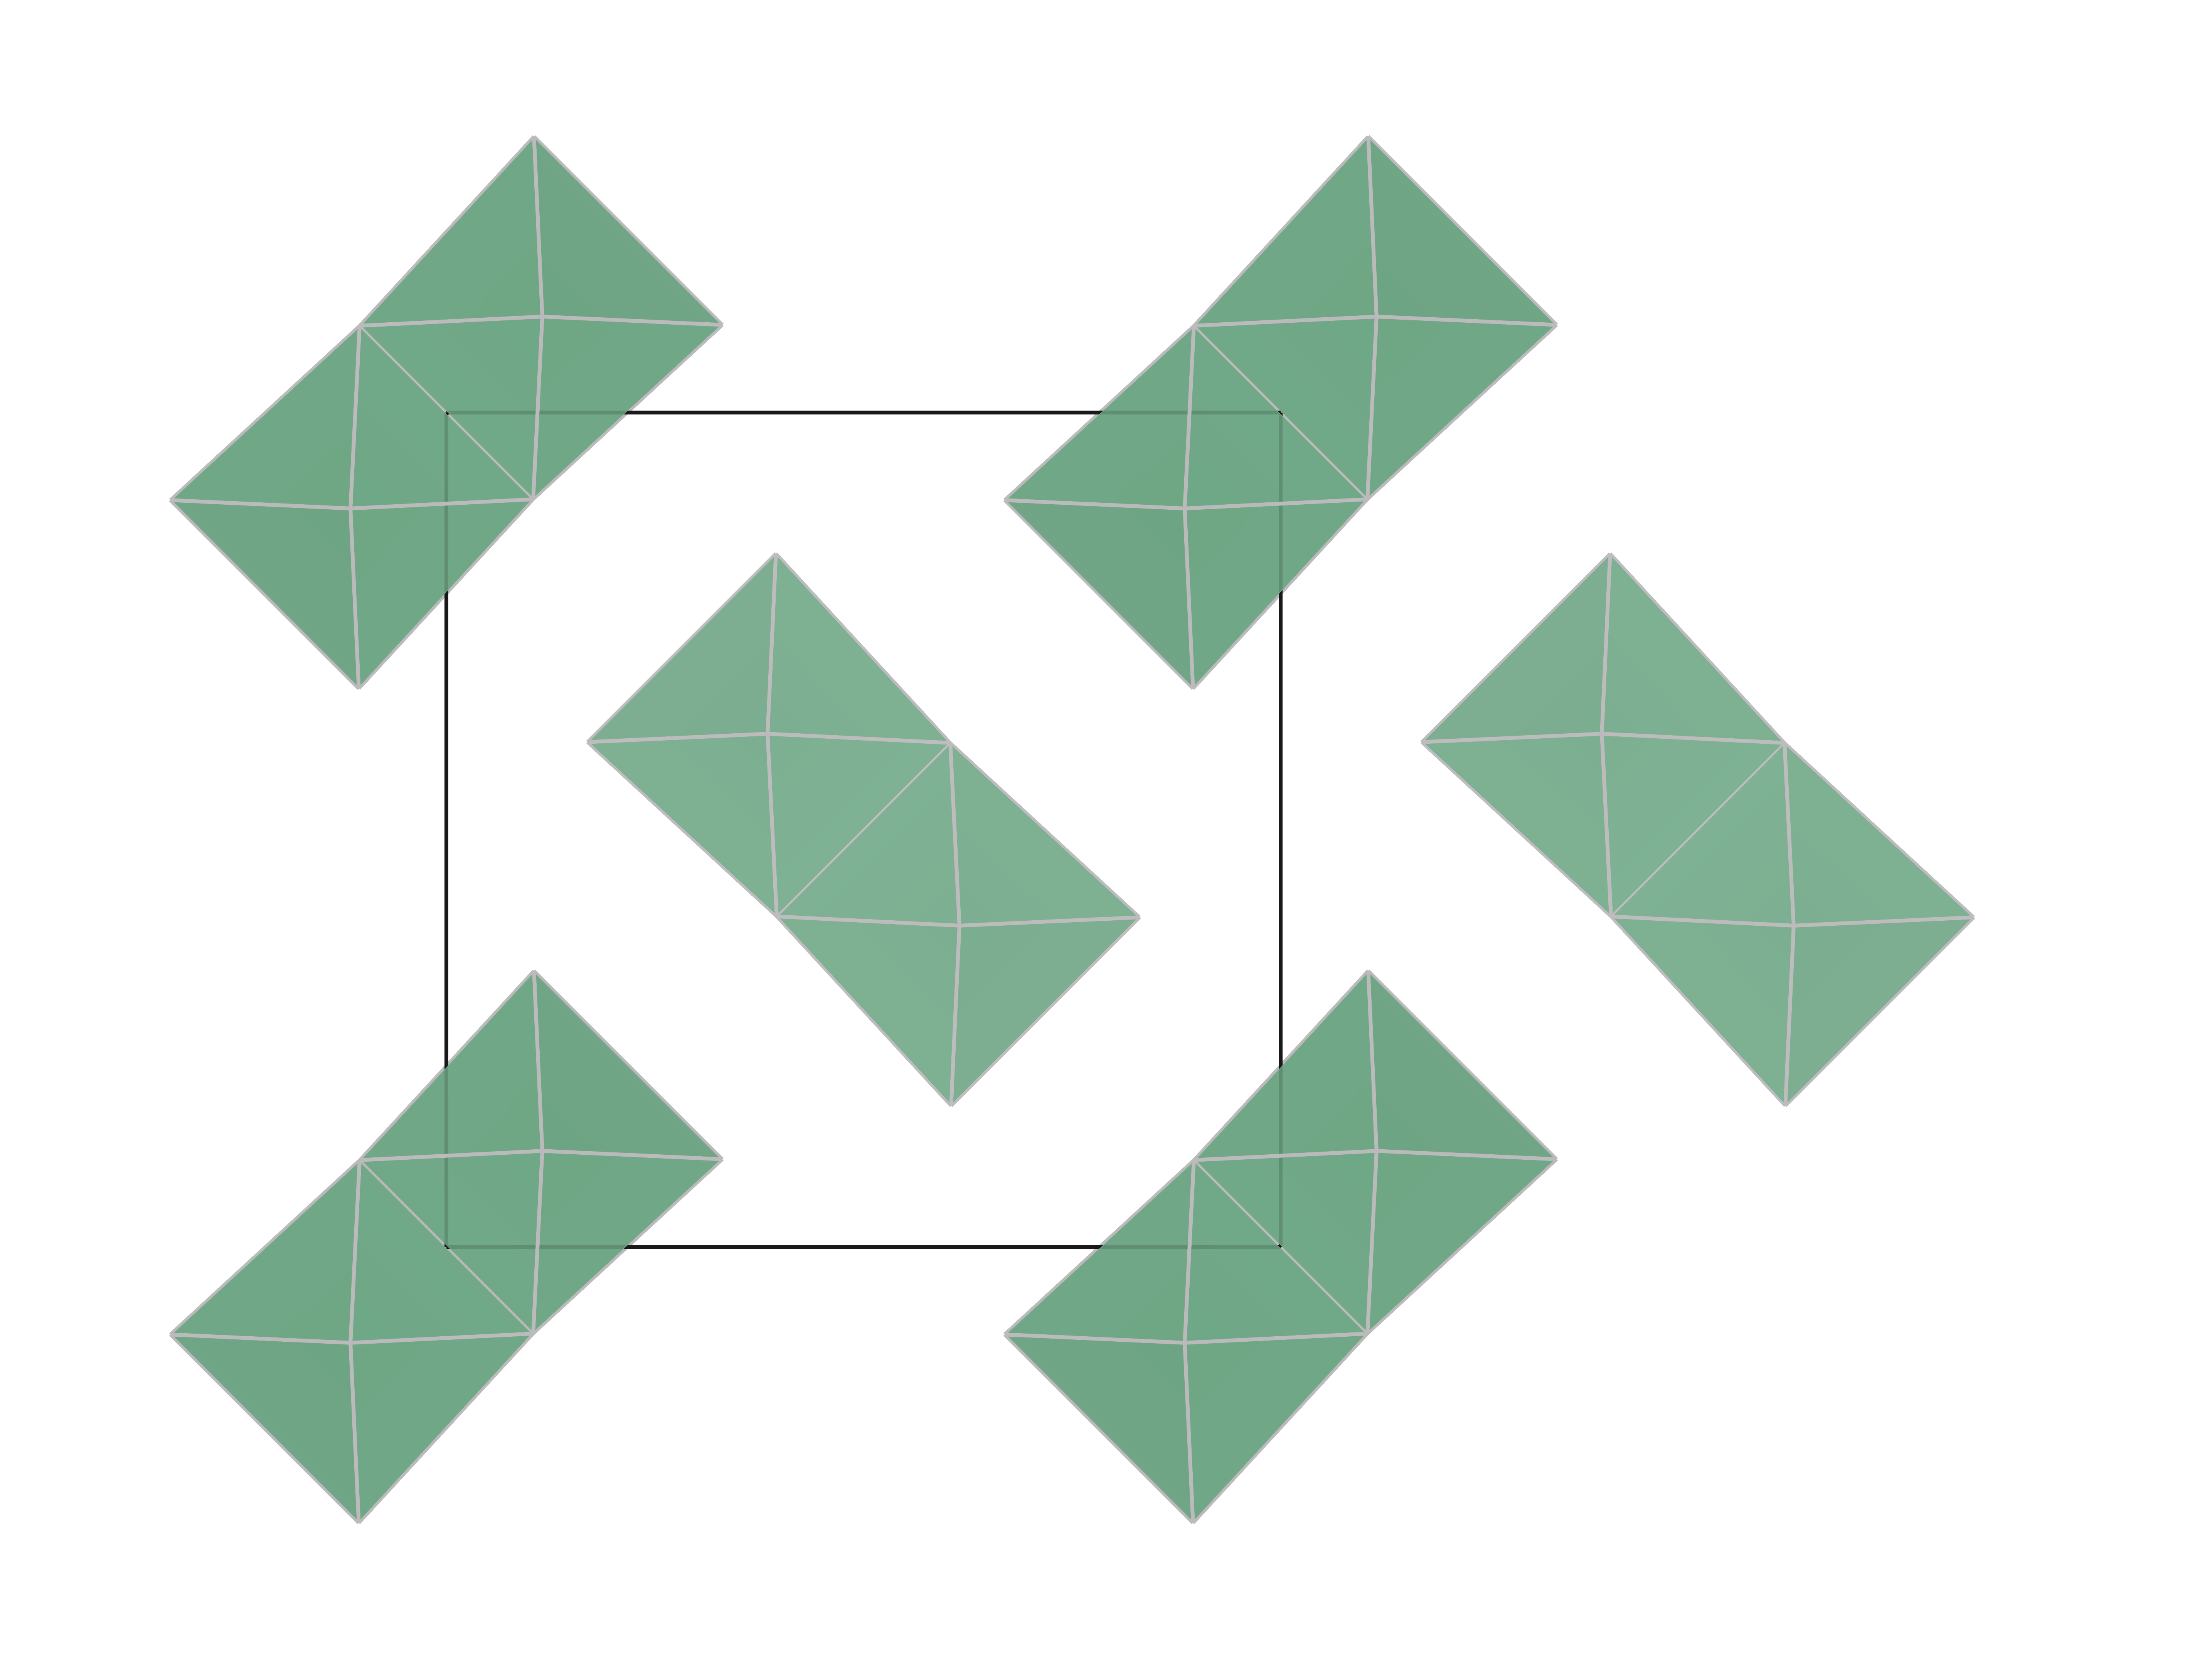
\includegraphics[scale=0.04]{Ch10/Rutile/NbOCl3}
	\caption{Structure and unit cell projection of $\rm NbOCl_3$}
	\label{nbocl3}
\end{figure}
%
\subsection{NiAs, CdI$_{\textbf{2}}$ and Corundums}
%
These three structures are all octahedra-filled hcp stackings with filling rate 100\%, 50\% and 2/3 respectively.
CdI$_2$ and corundums possess only a $\bar{3}$ without 6-fold axes due to the asymmetry of filling layers.\\ \\
%
In NiAs structure, Ni atoms are in the octahedral sites of As hcp, and As atoms are in trigonal prismatic interstices of Ni. 
$\rm [NiAs_6]$ octahedra share faces between layers and egdes within one layer.
Each octahedron is connected to 2 octahedra in $c$ direction and another 6 in $ab$ plane.\\ \\
%
Deriving $\rm CdI_2$ structure from NiAs, we take away half of the filling layers. The stacking-filling model expression for them is:
%
\[
	\text{NiAs }\ |\,A\,c\,B\,c\,|\,A\,c\,B\,c\,|\cdots
	\quad\Rightarrow\quad
	|\,A\,c\,B\,\square\,|\,A\,c\,B\,\square\,|\cdots\ \text{ CdI}_2
\]
Then the $\rm [CdI_6]$ octahedra are only connected with shared edges to another 6 within a layer.
The unit cells of these two structures, if we place the filling layers at vertices, are shown in figure \ref{nias}.\\
%
\begin{figure}[h]
	\centering
	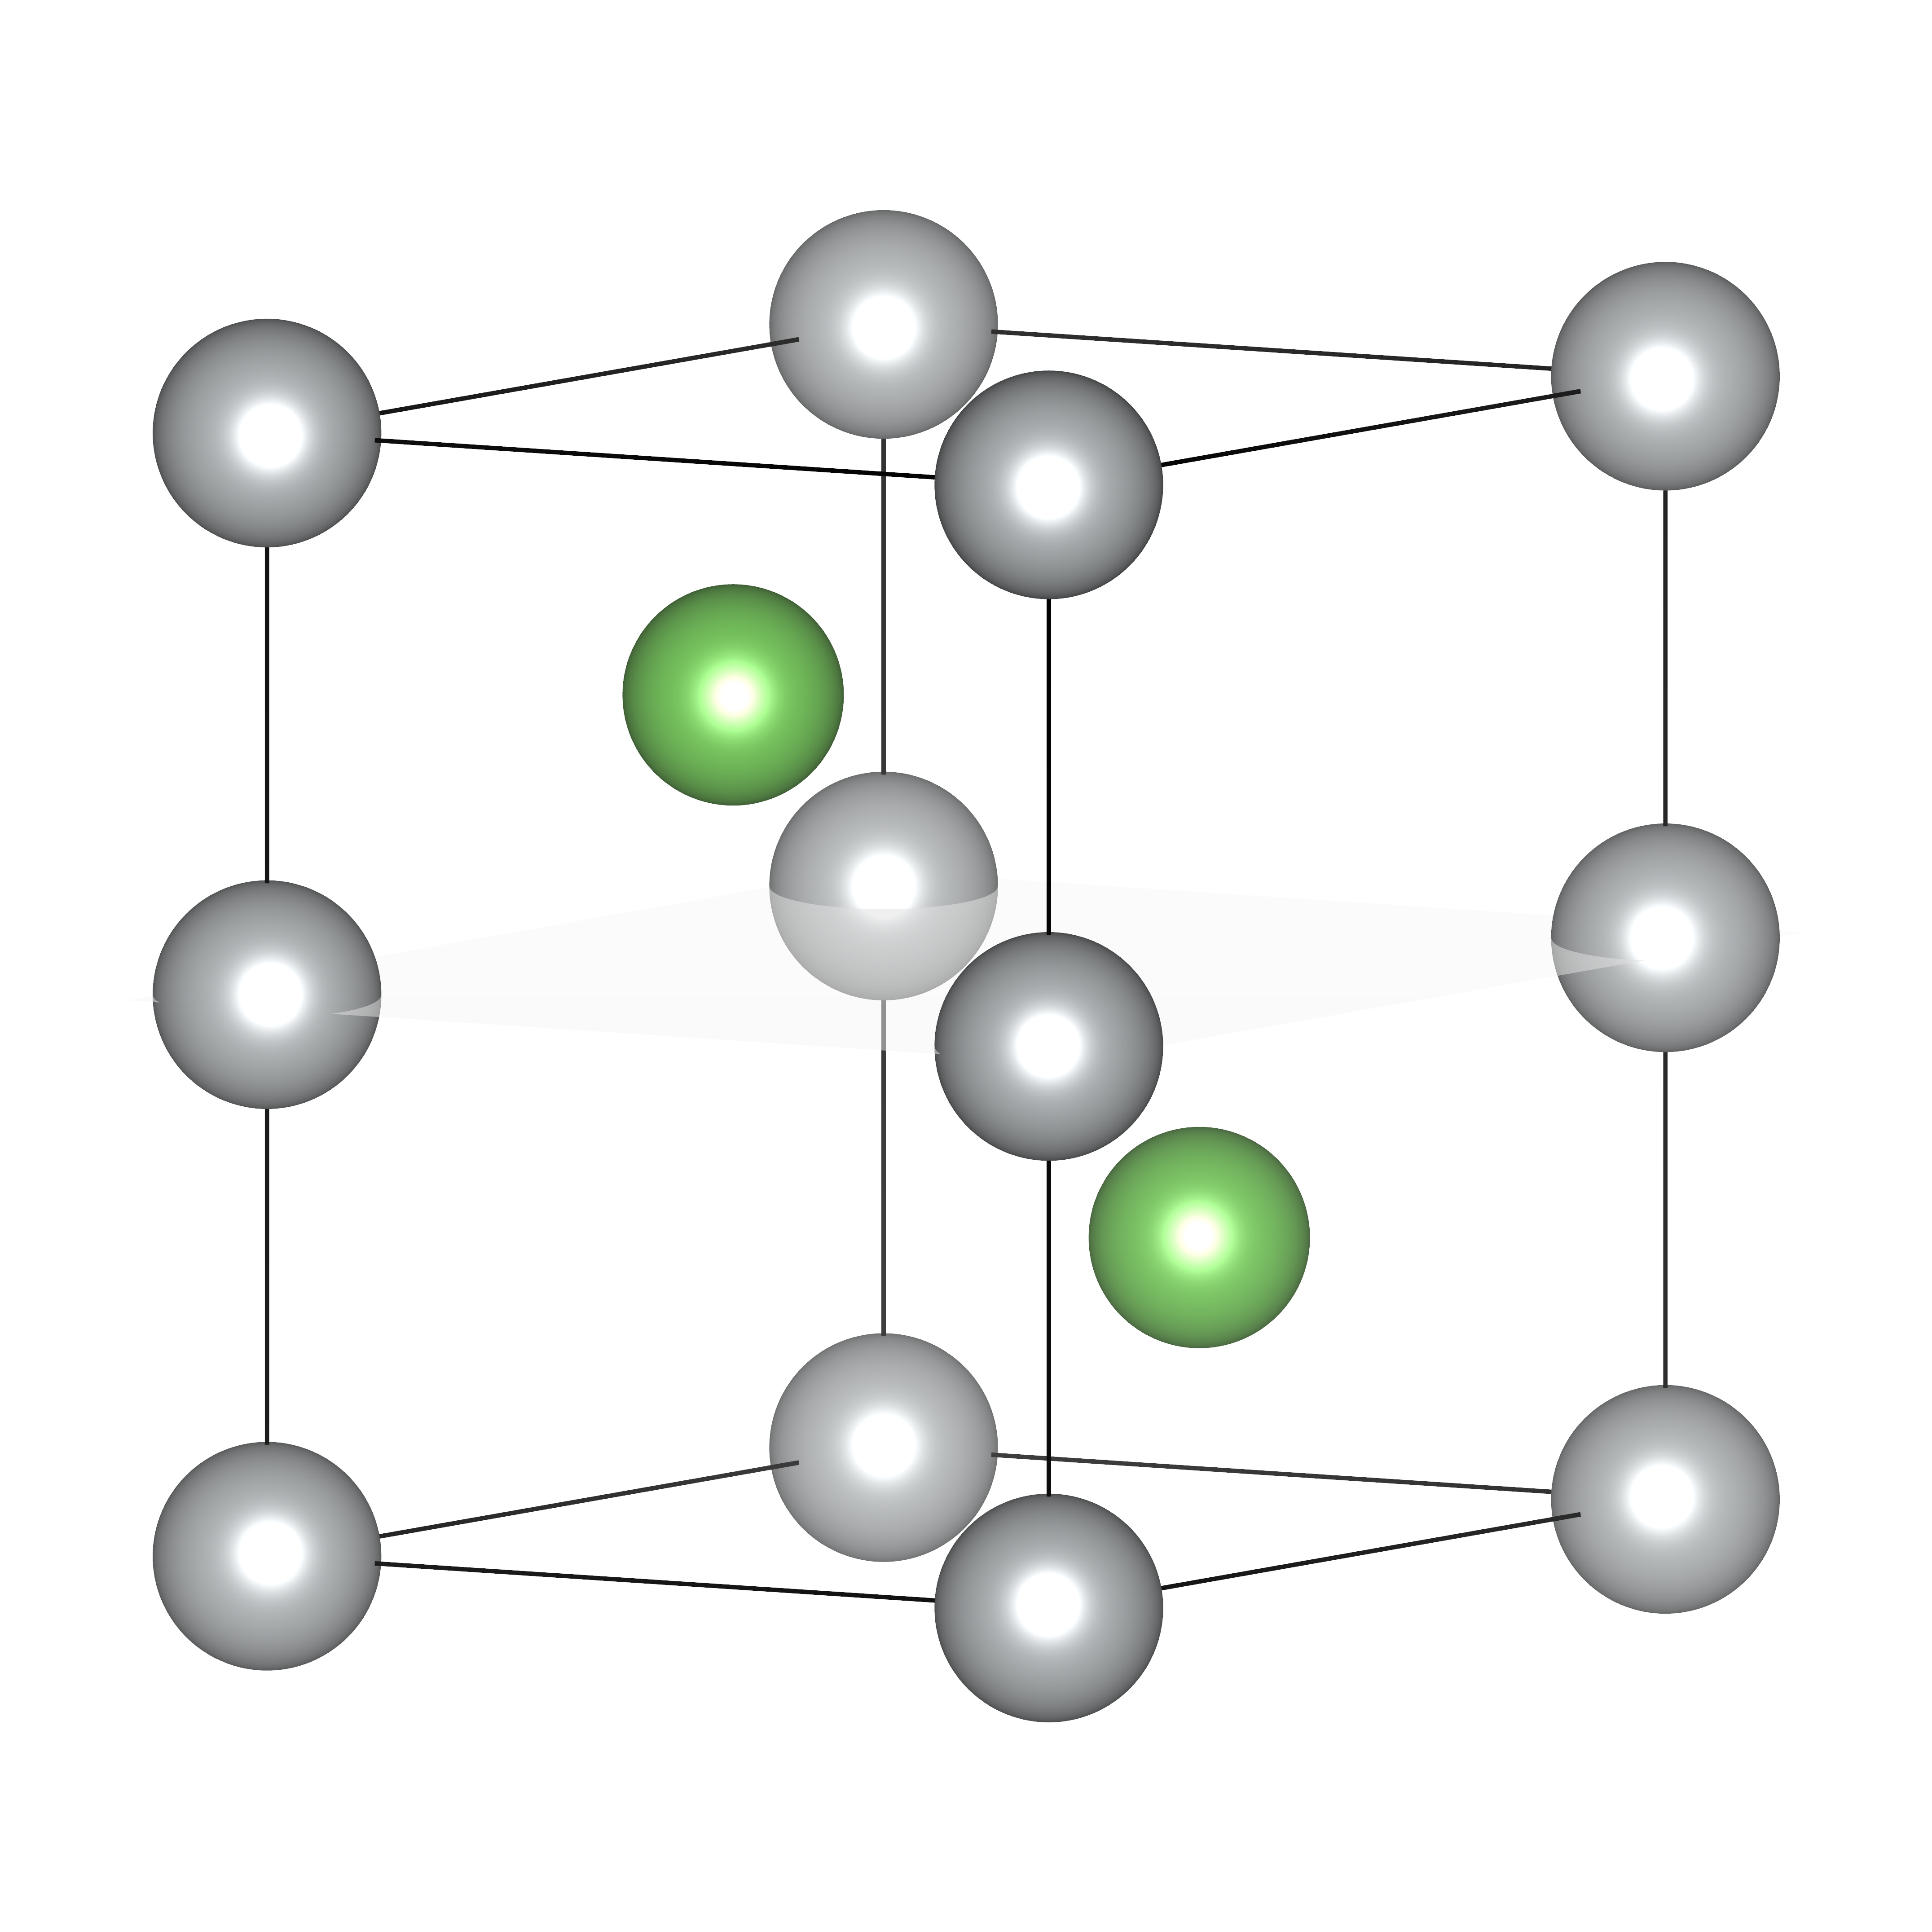
\includegraphics[scale=0.0361]{Ch10/Hexagonal/NiAs}
	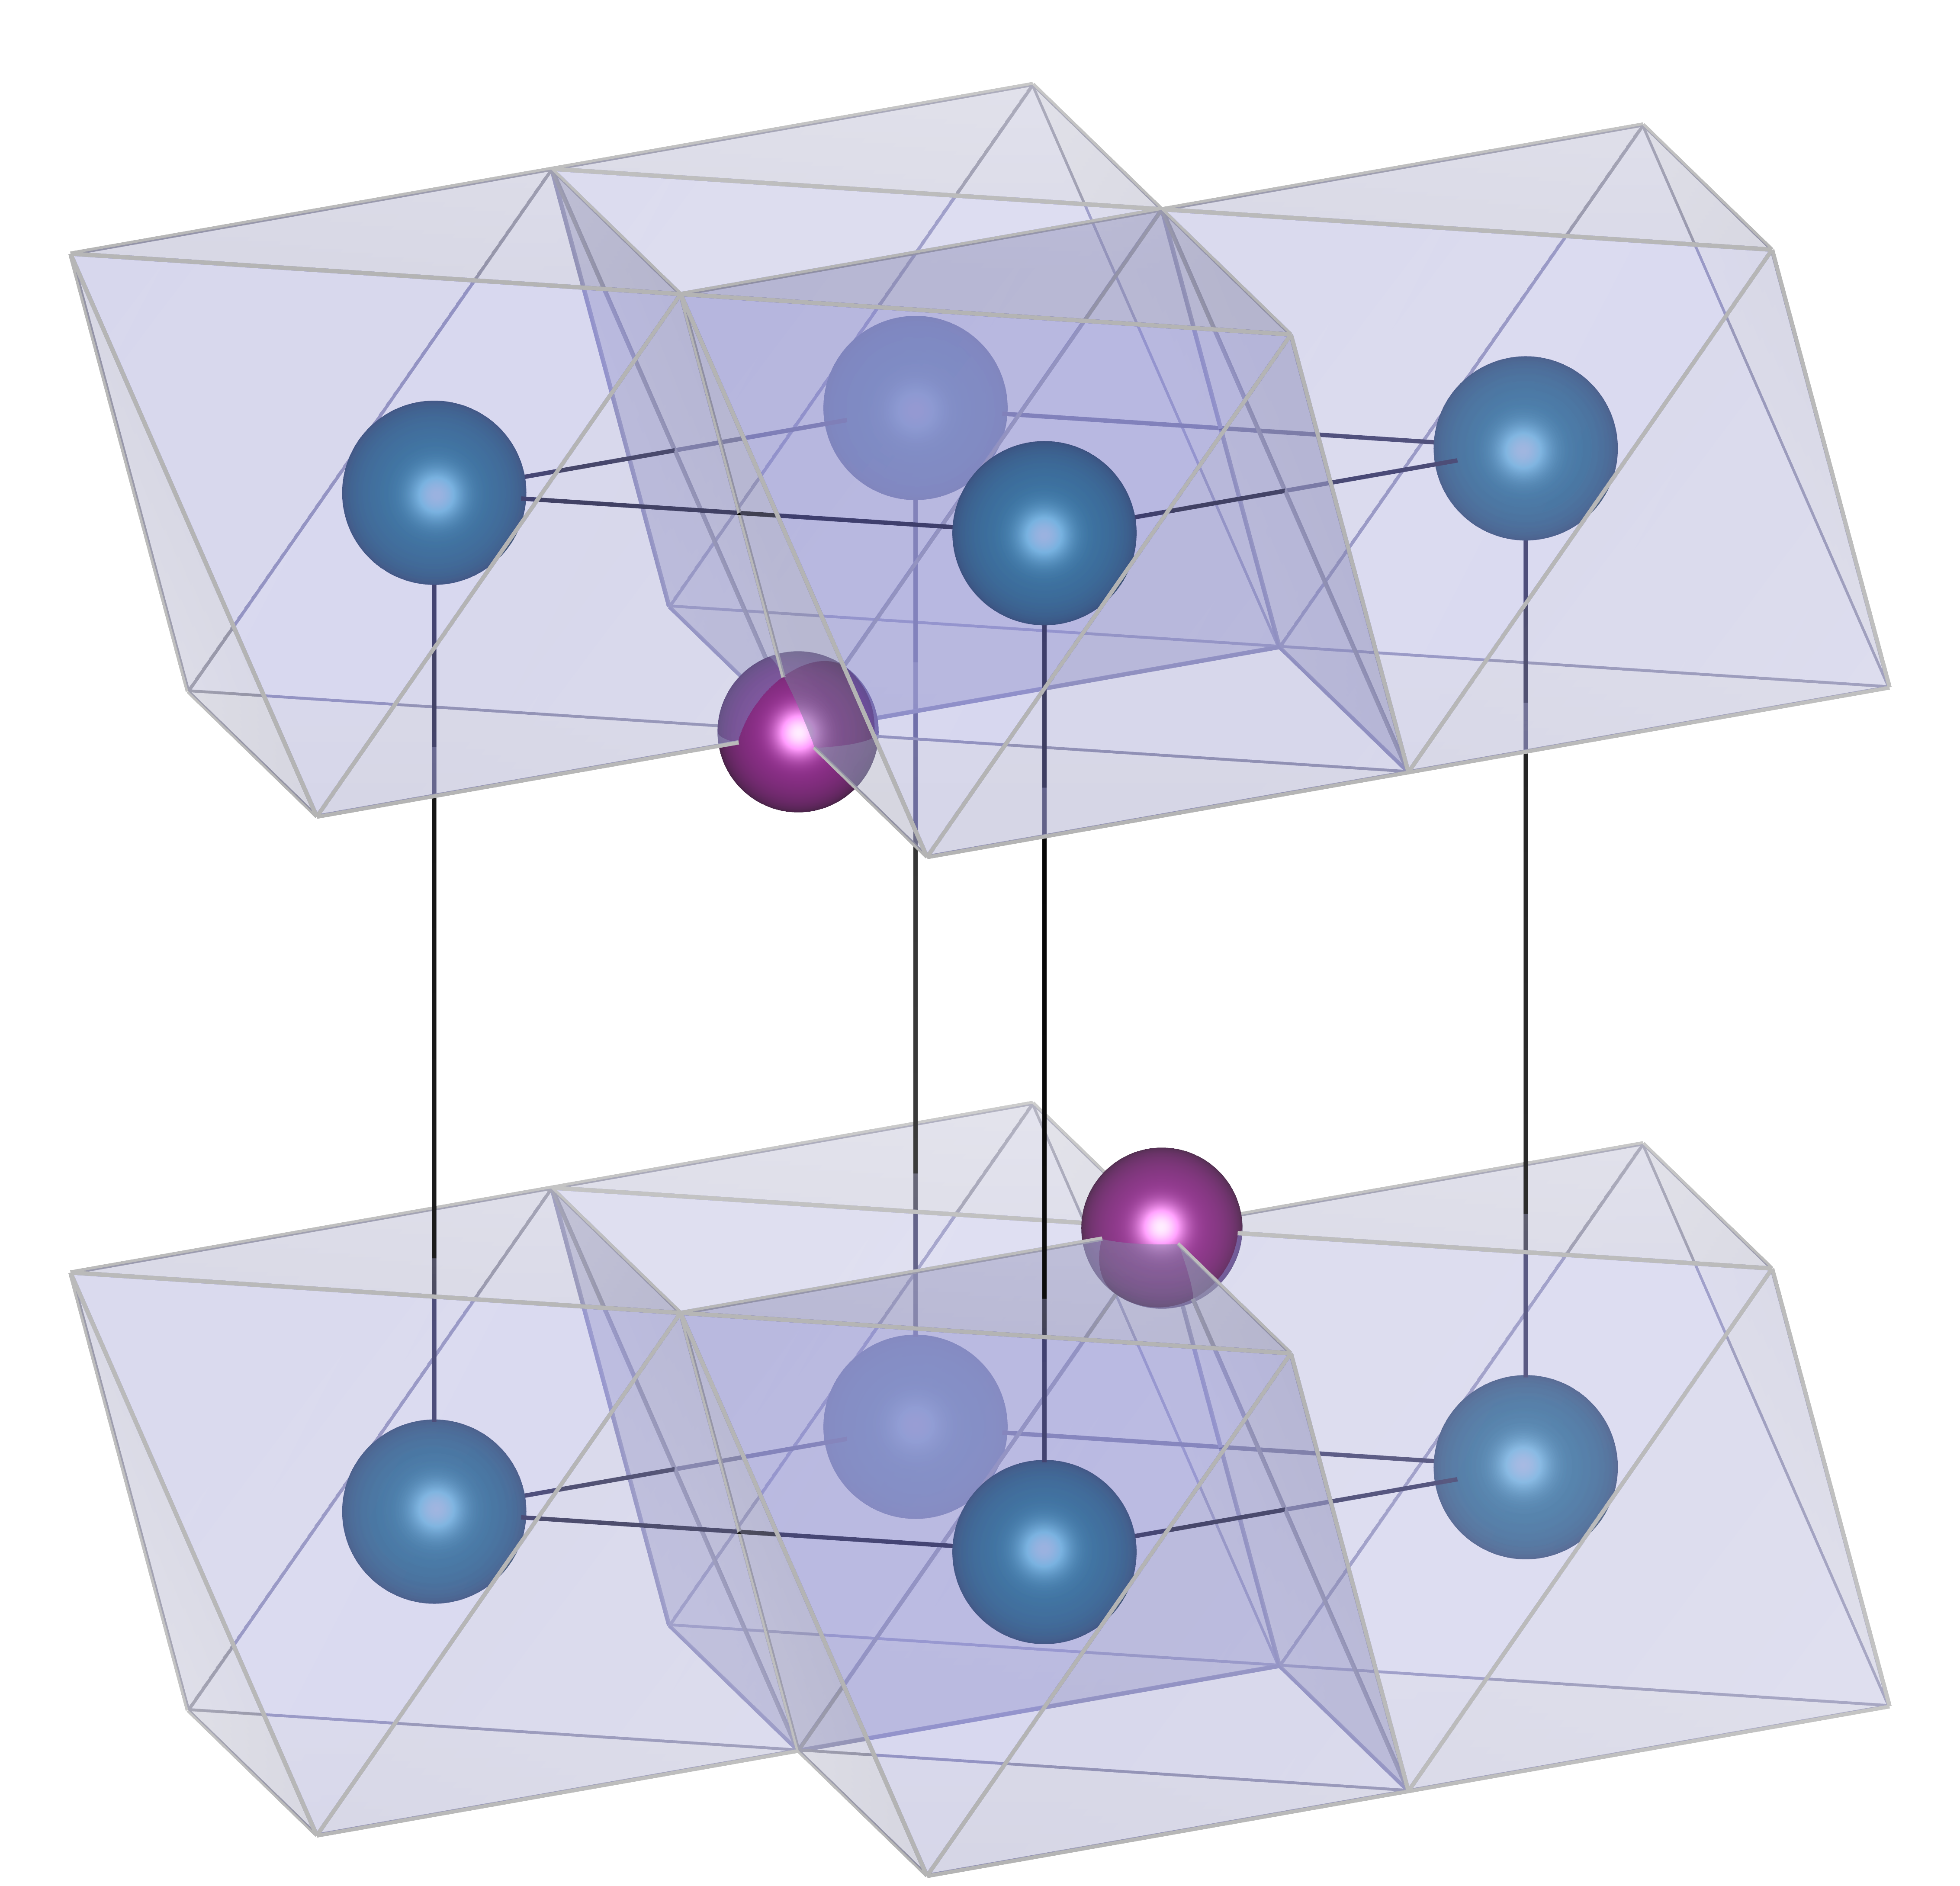
\includegraphics[scale=0.04]{Ch10/Hexagonal/CdI2}
	\caption{Unit cells of NiAs and $\rm CdI_2$}
	\label{nias}
\end{figure}\\
%
However filling 2/3 sites is a bit tricky. 
Symmetry doesn't allow a stacking paradigm of one vacant layer followed by two full filling layers.
Therefore we want a 2 dimensional cell 3 times larger than a simple hexagonal cell so that
there can be 3 atoms in one layer instead of 1.\\ \\ \\ \\
%
Note that the longer diagonal of a simple hexagonal cell is $\sqrt{3}a$, 
which means a hexagonal cell sided on the diagonal will be 3 times larger.
Hence we place the cell like figure \ref{al2o3cell}, where A and B layers are oxygen hcps and c's are the filling layers.\\
%
\begin{figure}[h]
	\centering
	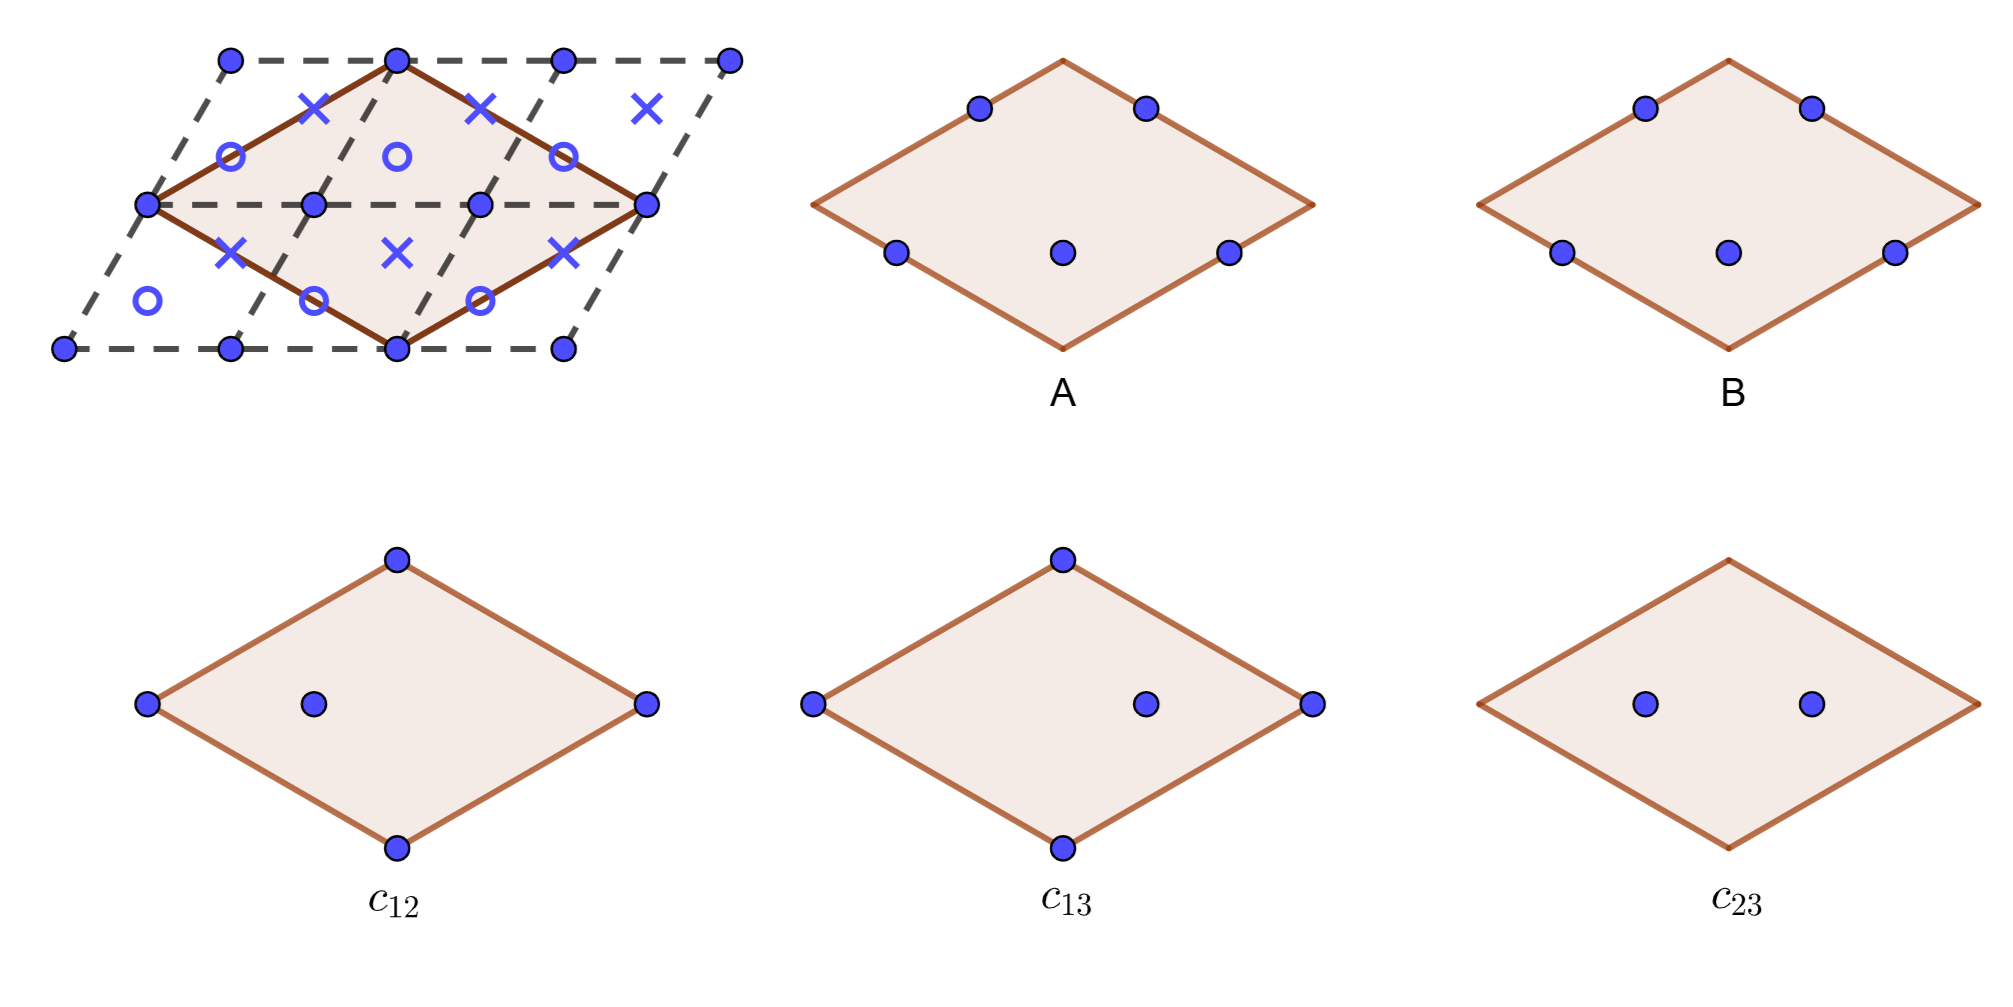
\includegraphics[scale=0.8]{Ch10/Hexagonal/Al2O3_layer}
	\caption{Layers in corundum structure}
	\label{al2o3cell}
\end{figure}\\
%
Thus the stacking-filling expression of corondums can be written as follows:
%
\[
	|\,A\,c_{12}\,B\,c_{23}\,A\,c_{13}\,B\,c_{12}\,A\,c_{23}\,B\,c_{13}\,|\cdots
\]
%
Focus on the paradigm of $\rm [AlO_6]$ octahedra connection, 
due to vacancies within filling layers, one octahedra only share edges with another 3 within one layer, forming hexagonal rings.
Every hole of the rings is capped with two octahedra, above and below, 
which also means that if a octahedron shares a face with another one, say above, then a vacancy must be there below it.\\ \\
%
Nevertheless, due to the existence of vacancies, Al atoms are not exactly coplanar as 
they will distort towards vacancies to reduce Al-Al electrostatic repulsion.
The structure of corundums, also adopted by many $\rm X_2O_3$ oxides, 
and one hexagonal-ring structure layer of octahedra are shown in figure \ref{al2o3}.\\
%
\begin{figure}[h]
	\centering
	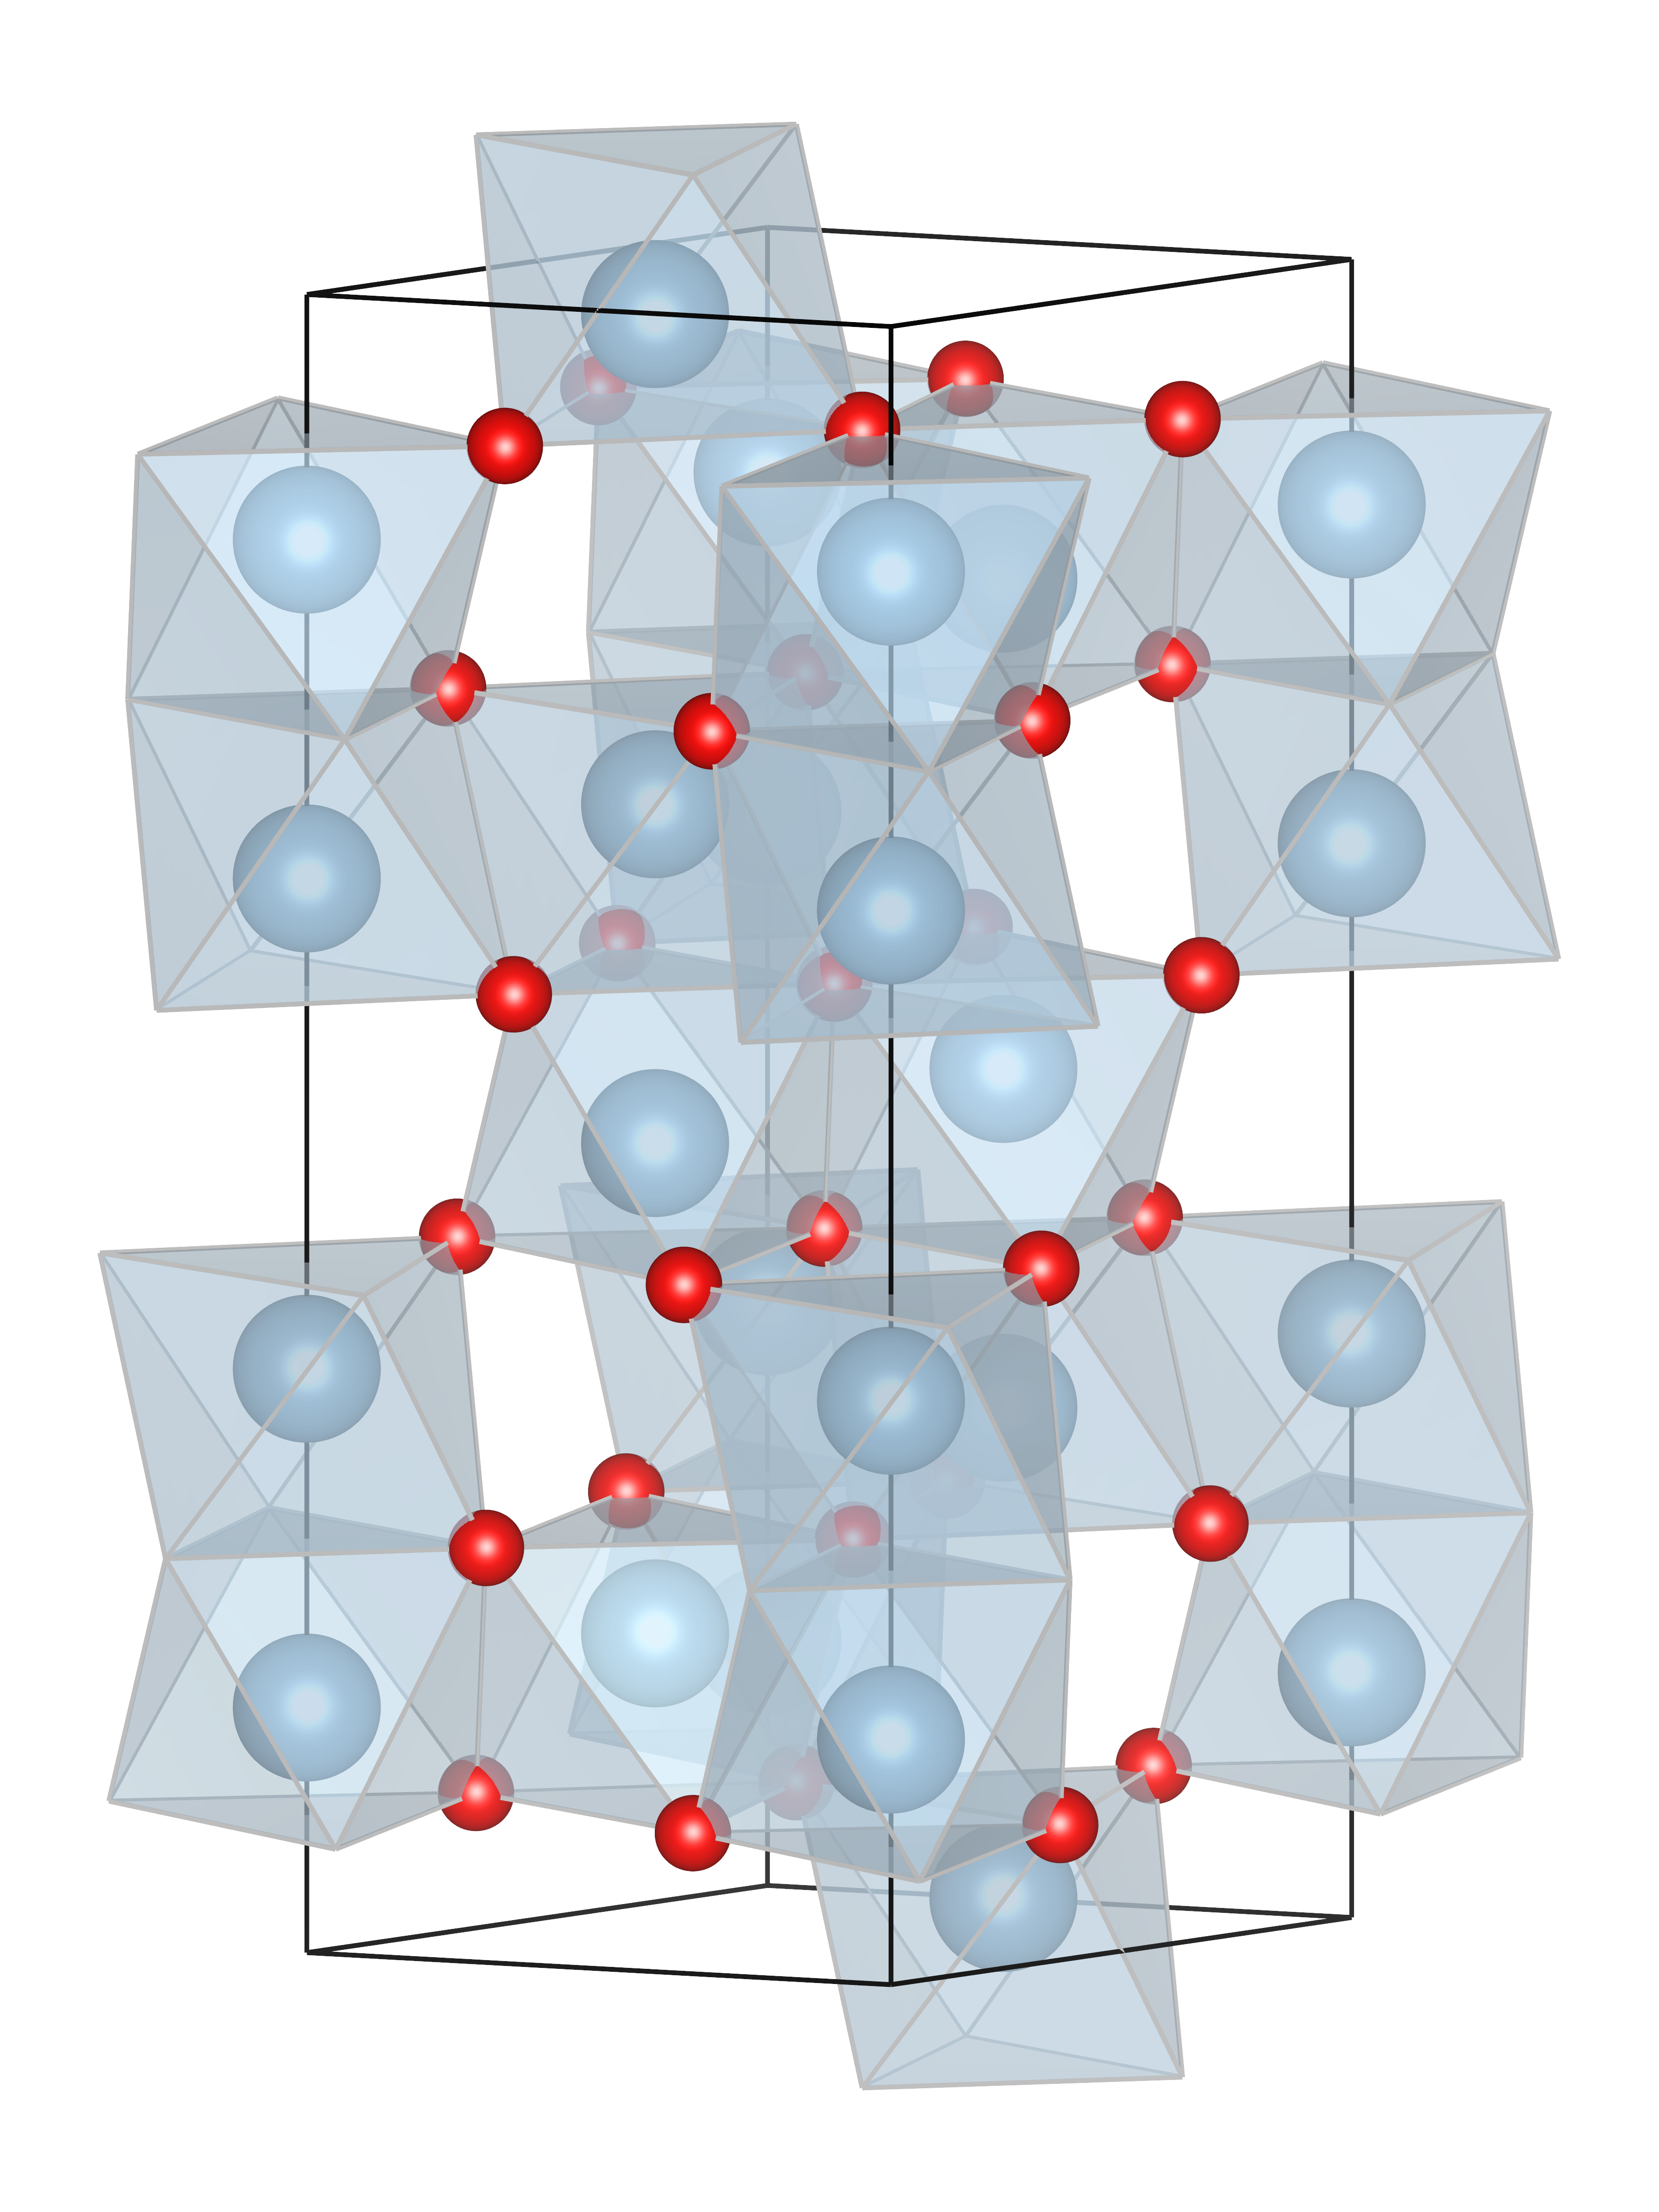
\includegraphics[scale=0.05]{Ch10/Hexagonal/Al2O3}
	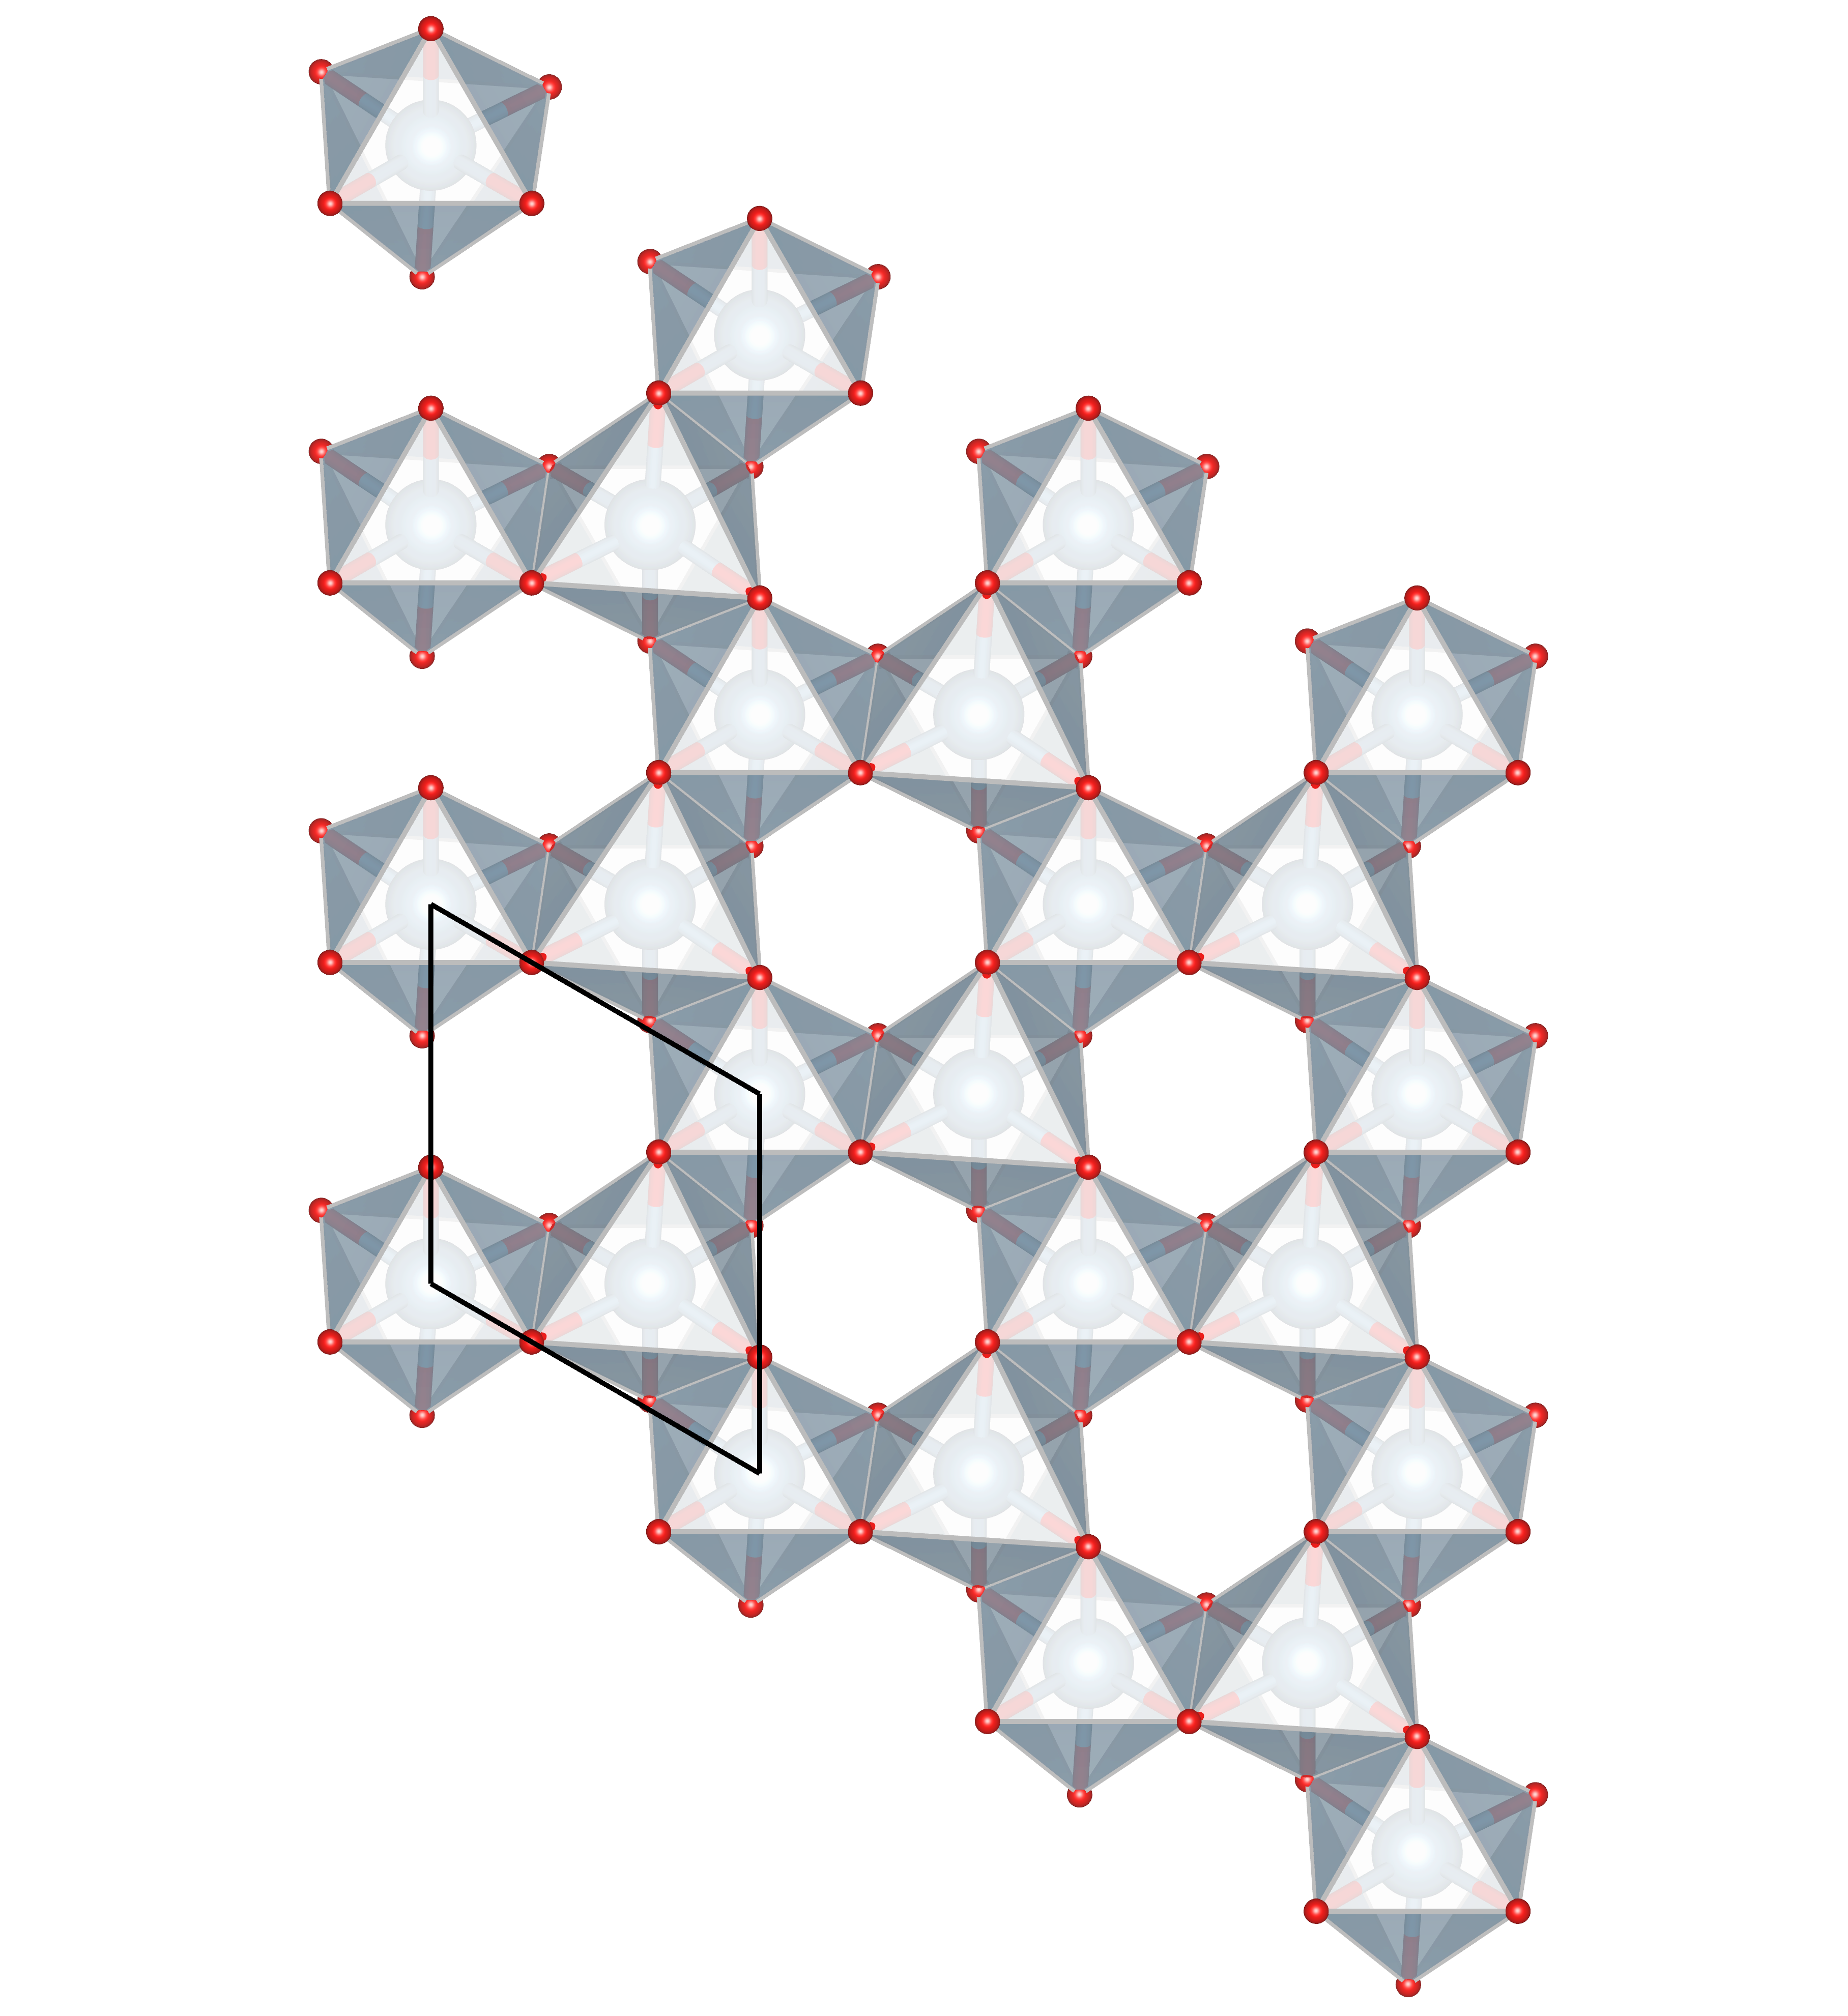
\includegraphics[scale=0.055]{Ch10/Hexagonal/Al2O3_ring}
	\caption{Unit cell and layer structure of corundums}
	\label{al2o3}
\end{figure}\ \\
%
The structures of graphite resemble that of corundum octahedra layer. 
Hexagonal graphite can be considered as stackings of $c_{12}$ and $c_{23}$ layers while trigonal graphite the stackings of all three.\\ \\ \\
Their unit cells are illustrated in figure \ref{graphite}.\\
%
\begin{figure}[h]
	\centering
	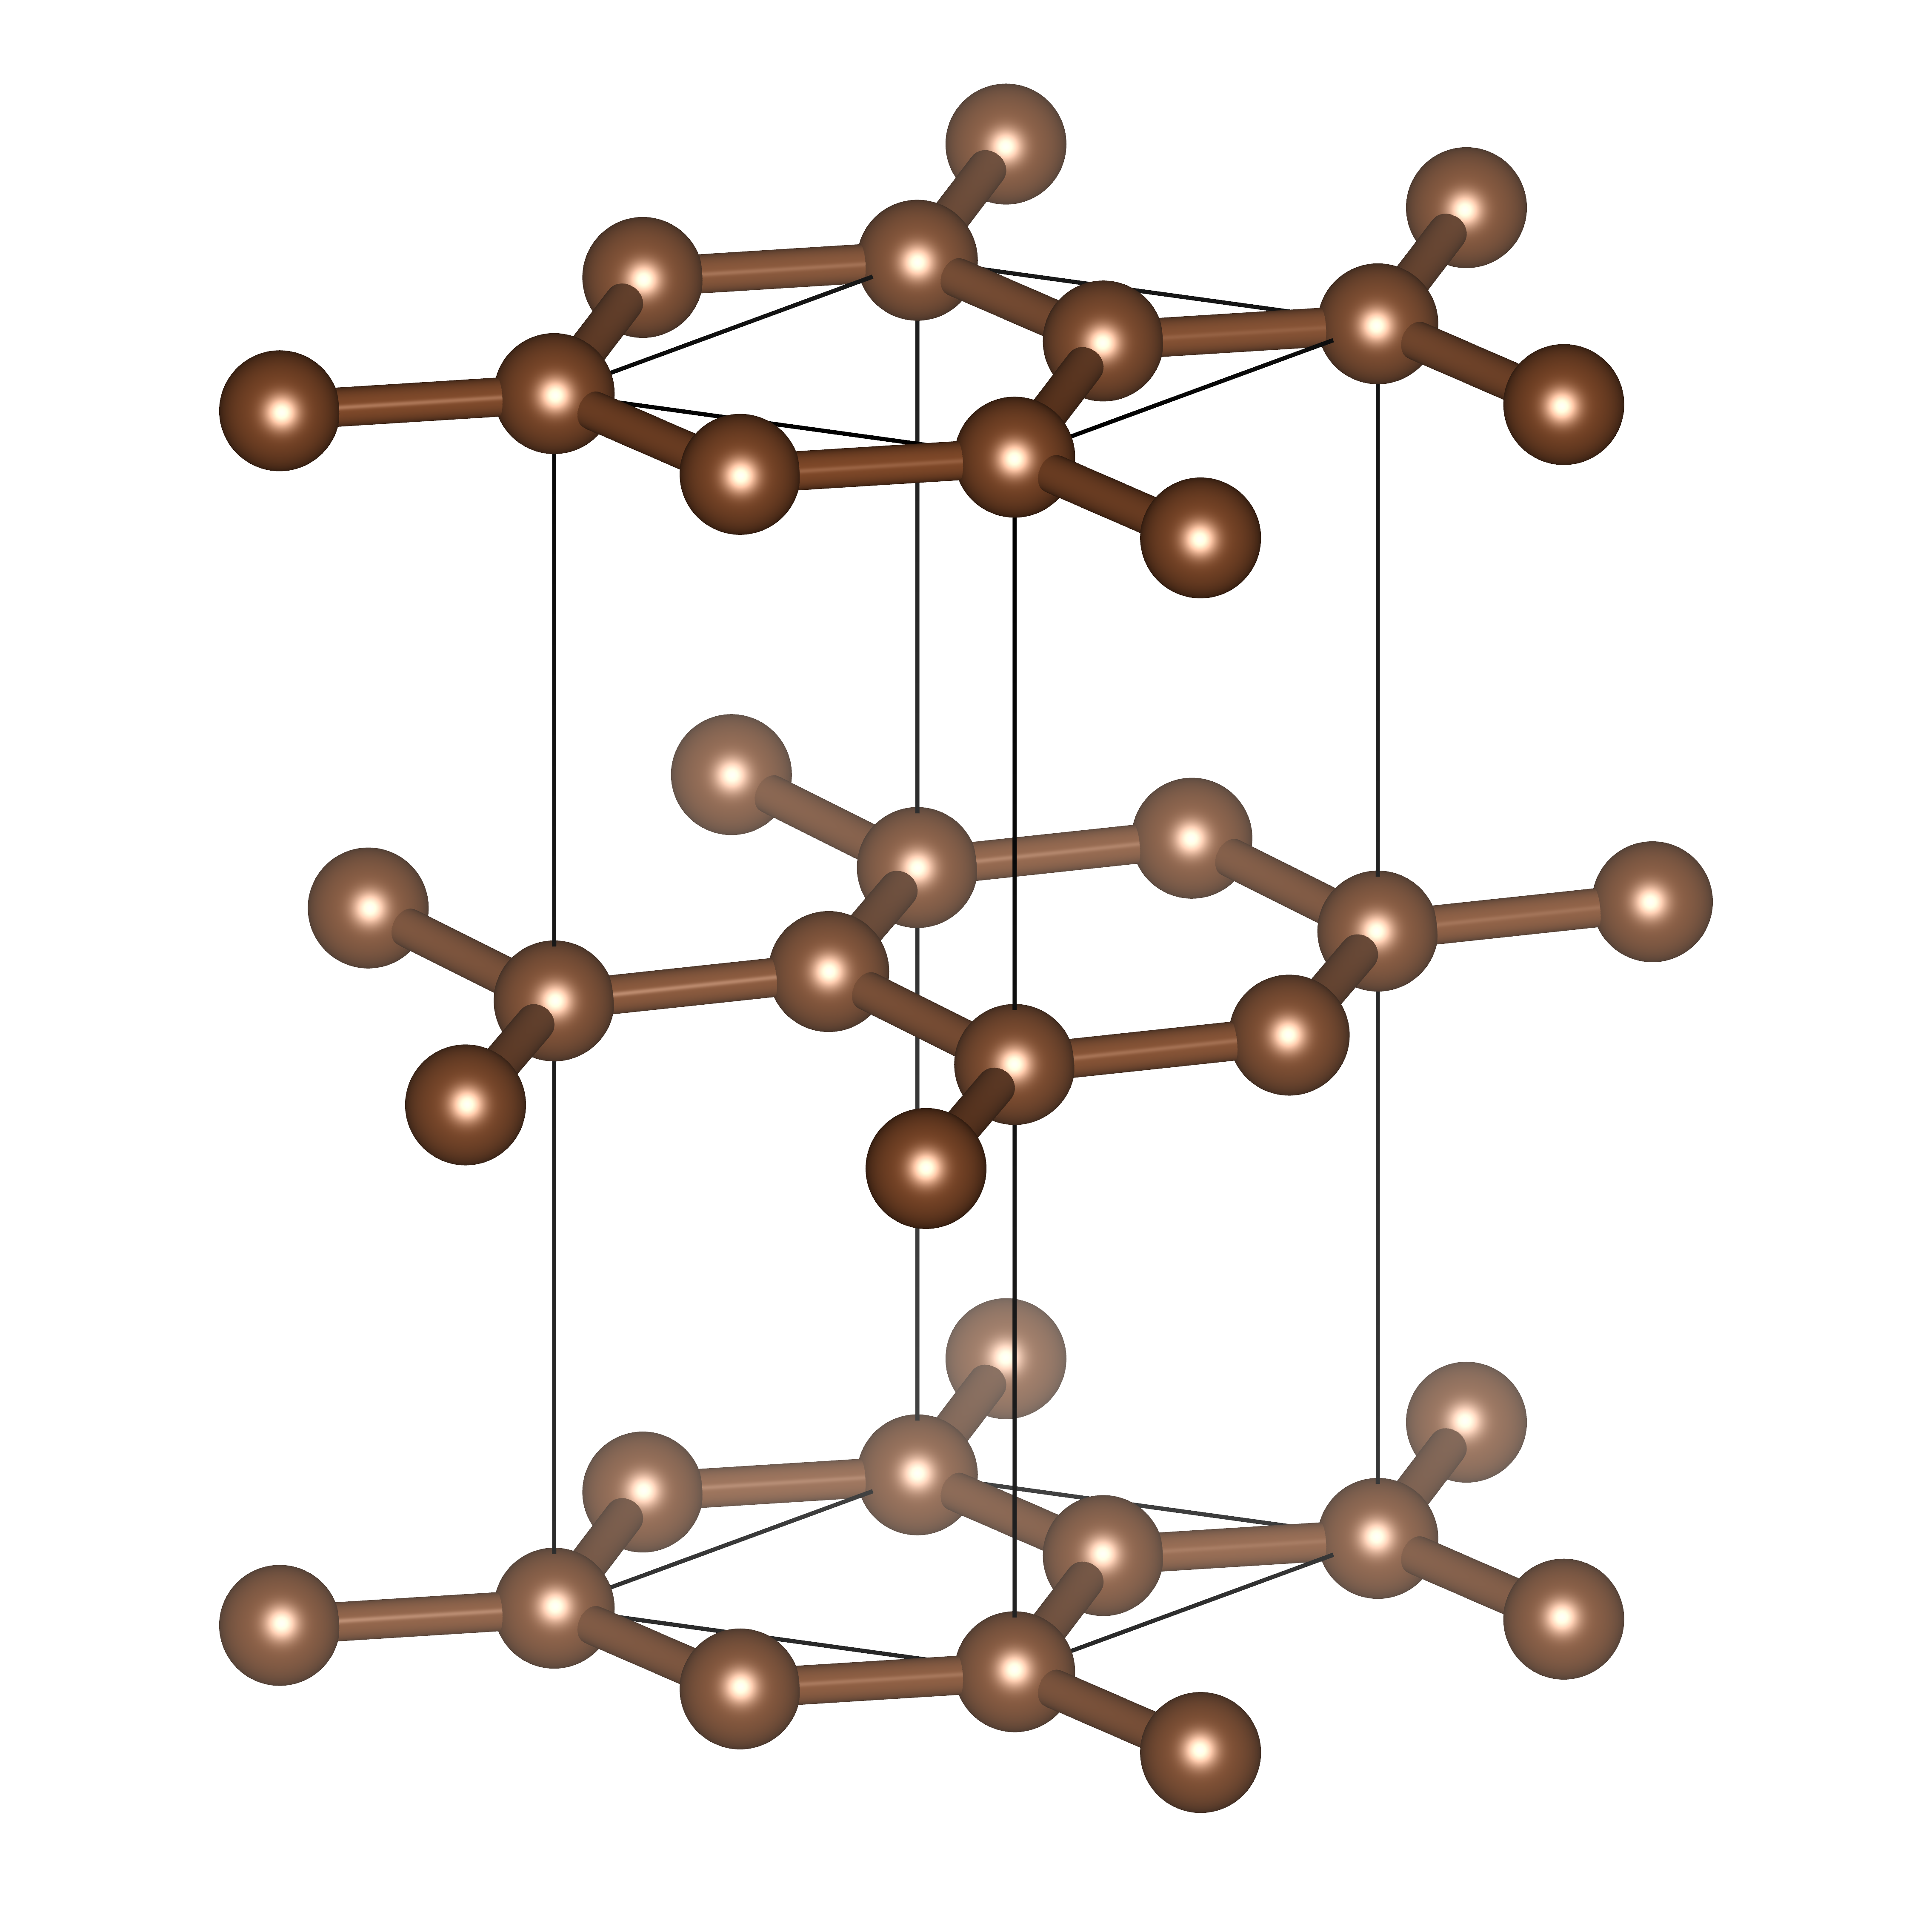
\includegraphics[scale=0.04]{Ch10/Hexagonal/Hgraphite}
	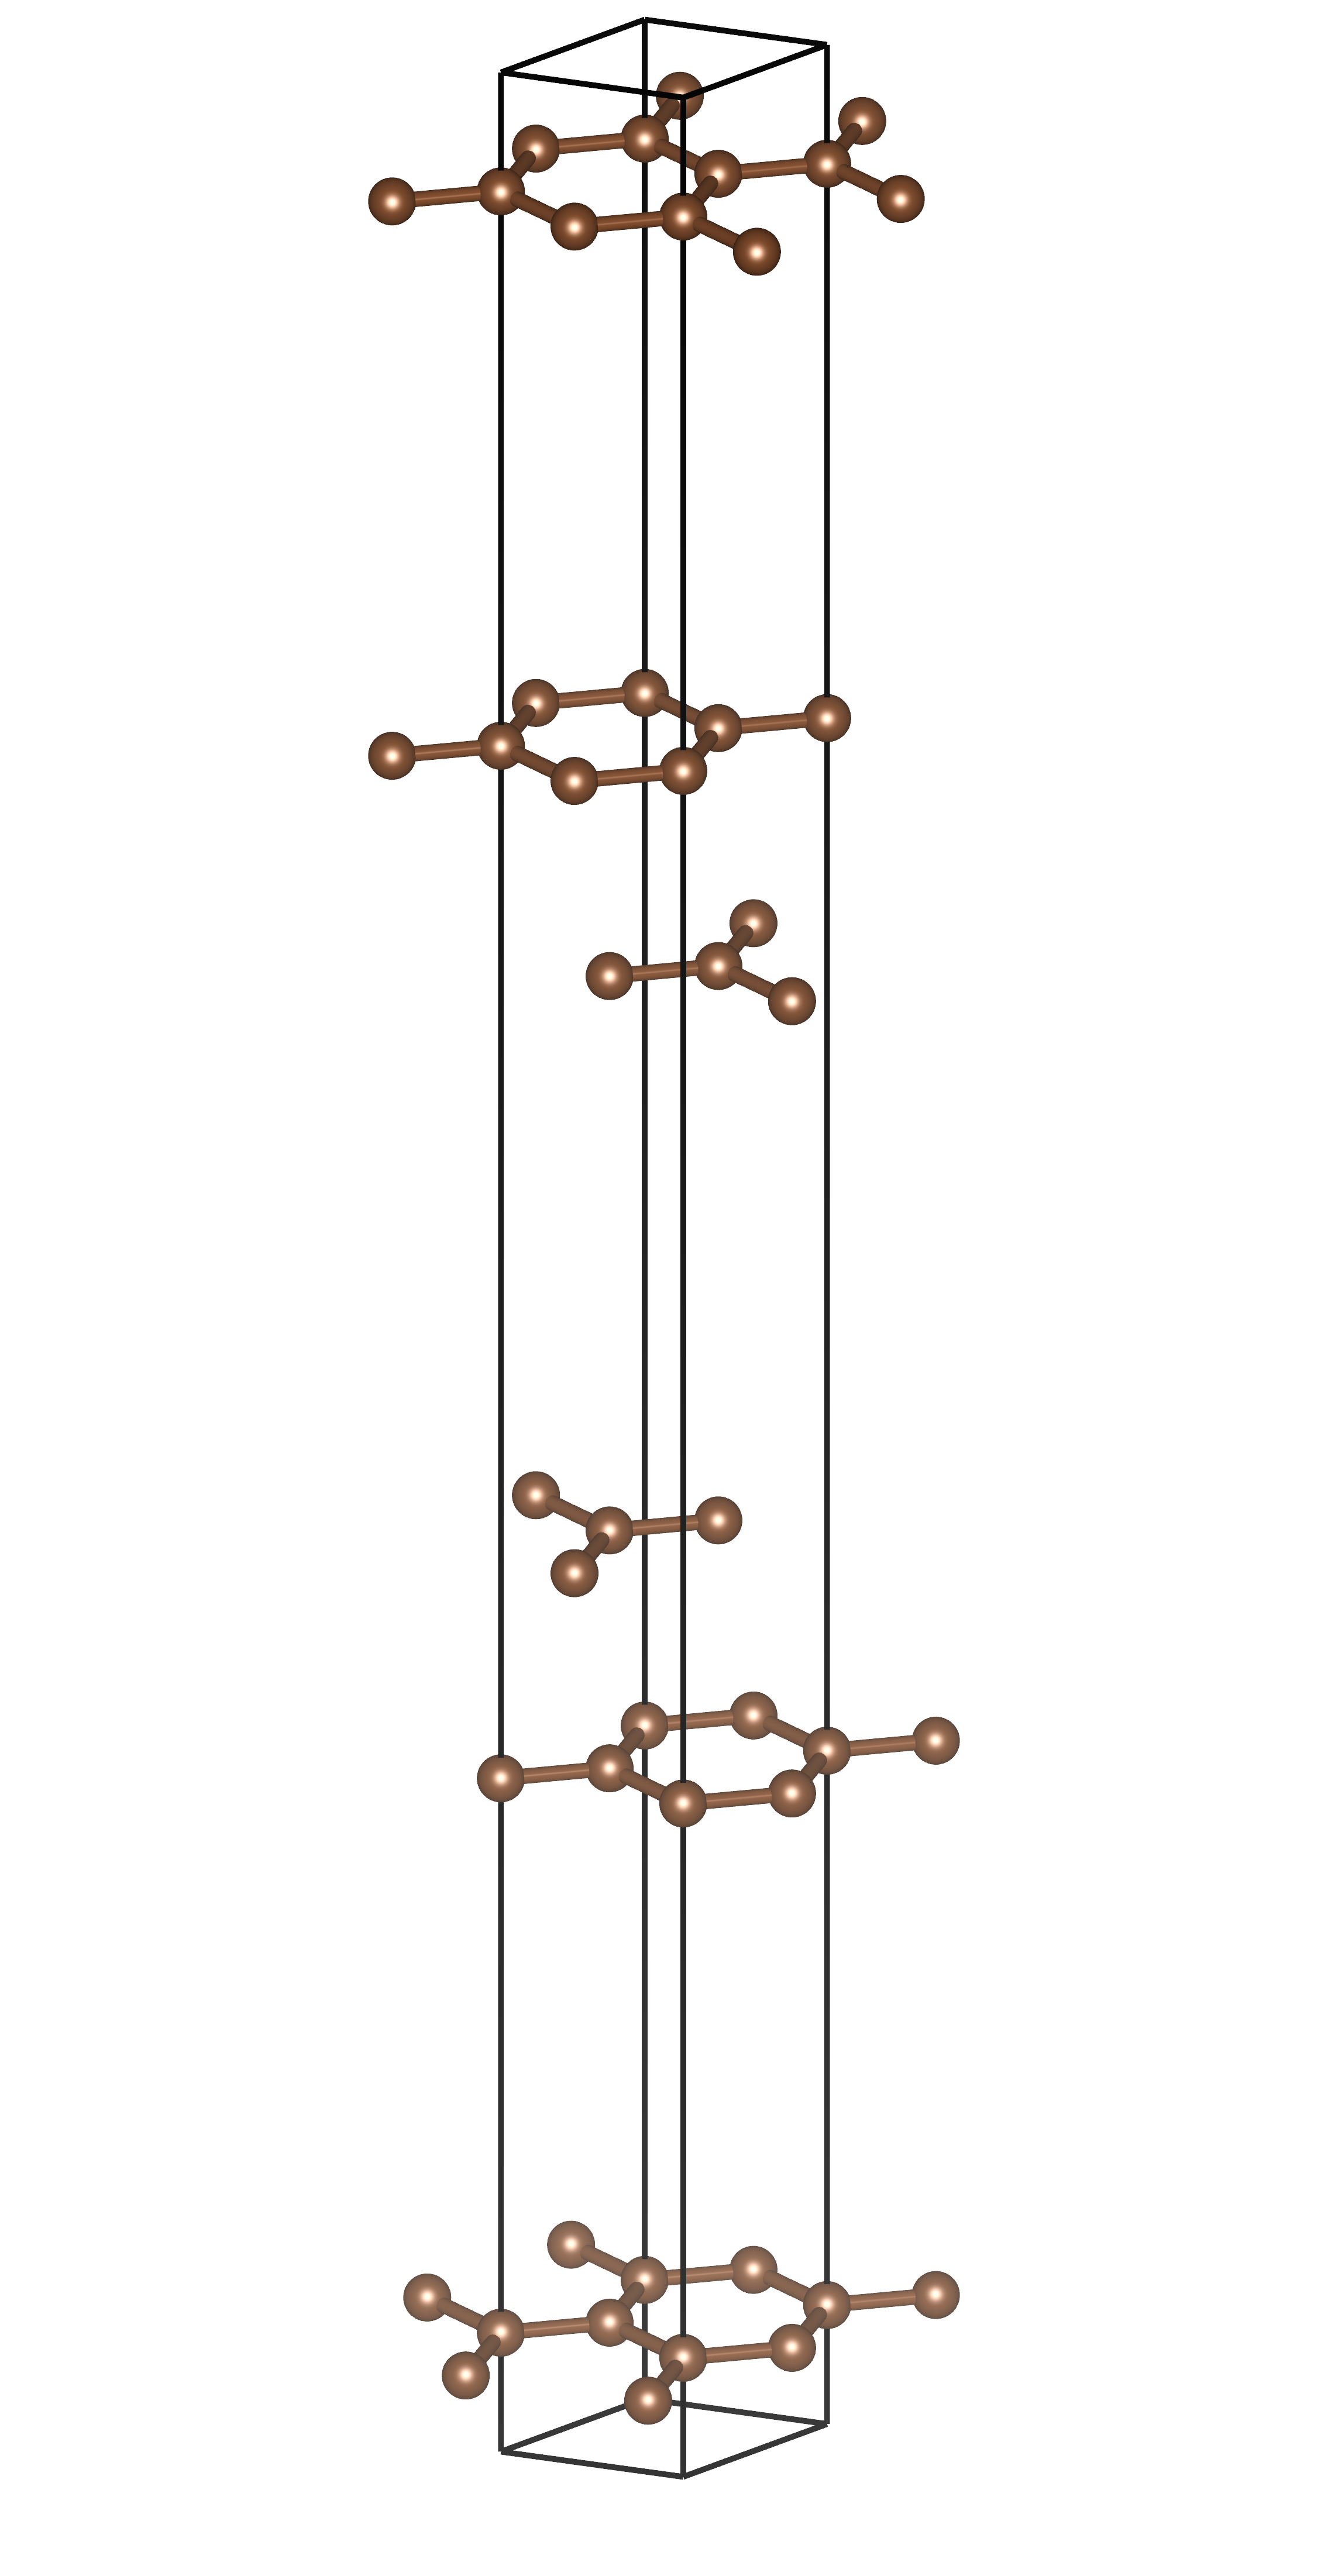
\includegraphics[scale=0.05]{Ch10/Hexagonal/Tgraphite}
	\caption{Unit cells of (a) hexagonal graphites (b) one type of trigonal graphite}
	\label{graphite}
\end{figure}
%
\subsection{Sphalerites, Wurtzites and Fluorites}
%
These three structures are all closest-packing with filled tetrahedral sites, filling rate 50\%, 50\% and 100\% respectively.
Wurtzites are hcp while the others are ccp. 
In every filling layer of sphalerites and wurtzites, only one kind of tetrahedral sites are occupied (see \ref{tetrahedralsite}).\\ \\
%
For sphalerites, if the filling atoms are the same as stacking atoms, they become diamond structures. 
Furthermore, substitution of atoms with symmetrically compatible patterns will also do, 
one example is $\rm [SiO_4]$ tetrahedron forms crystalline $\rm SiO_2$.
Figure \ref{sphalerite} illustrates these structures.\\
%
\begin{figure}[h]
	\centering
	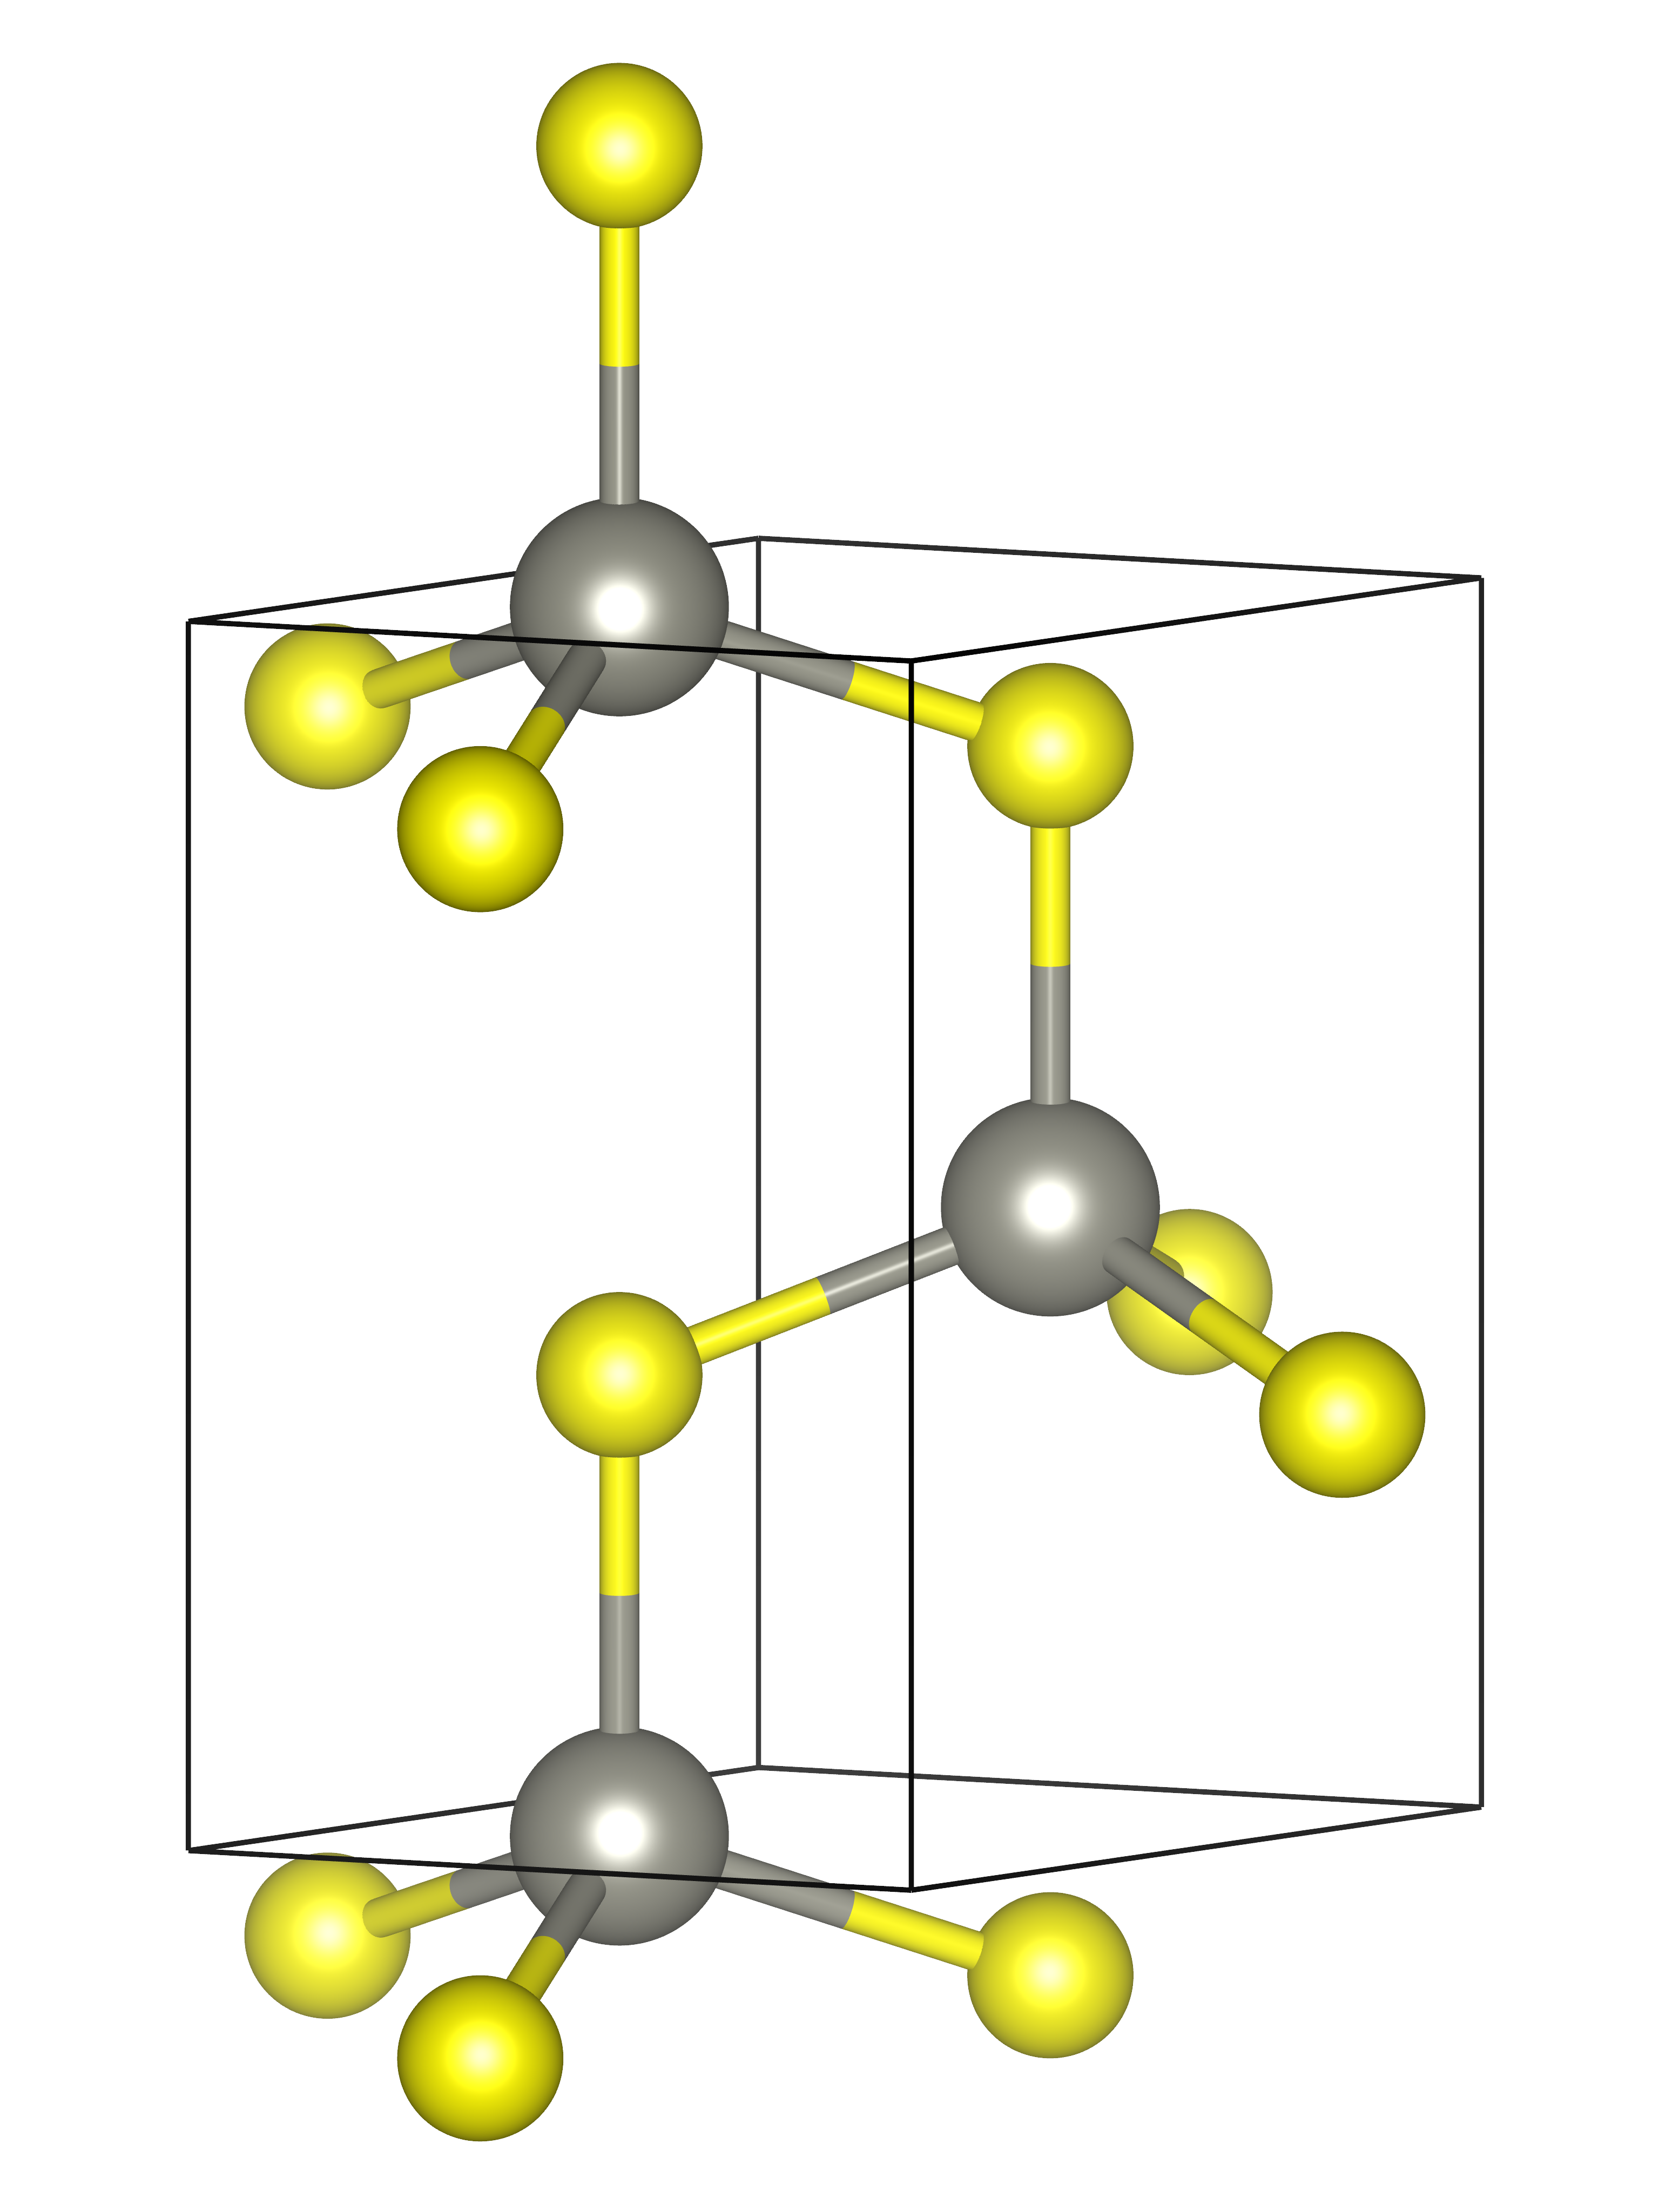
\includegraphics[scale=0.04]{Ch10/Cubic/ZnS_2}
	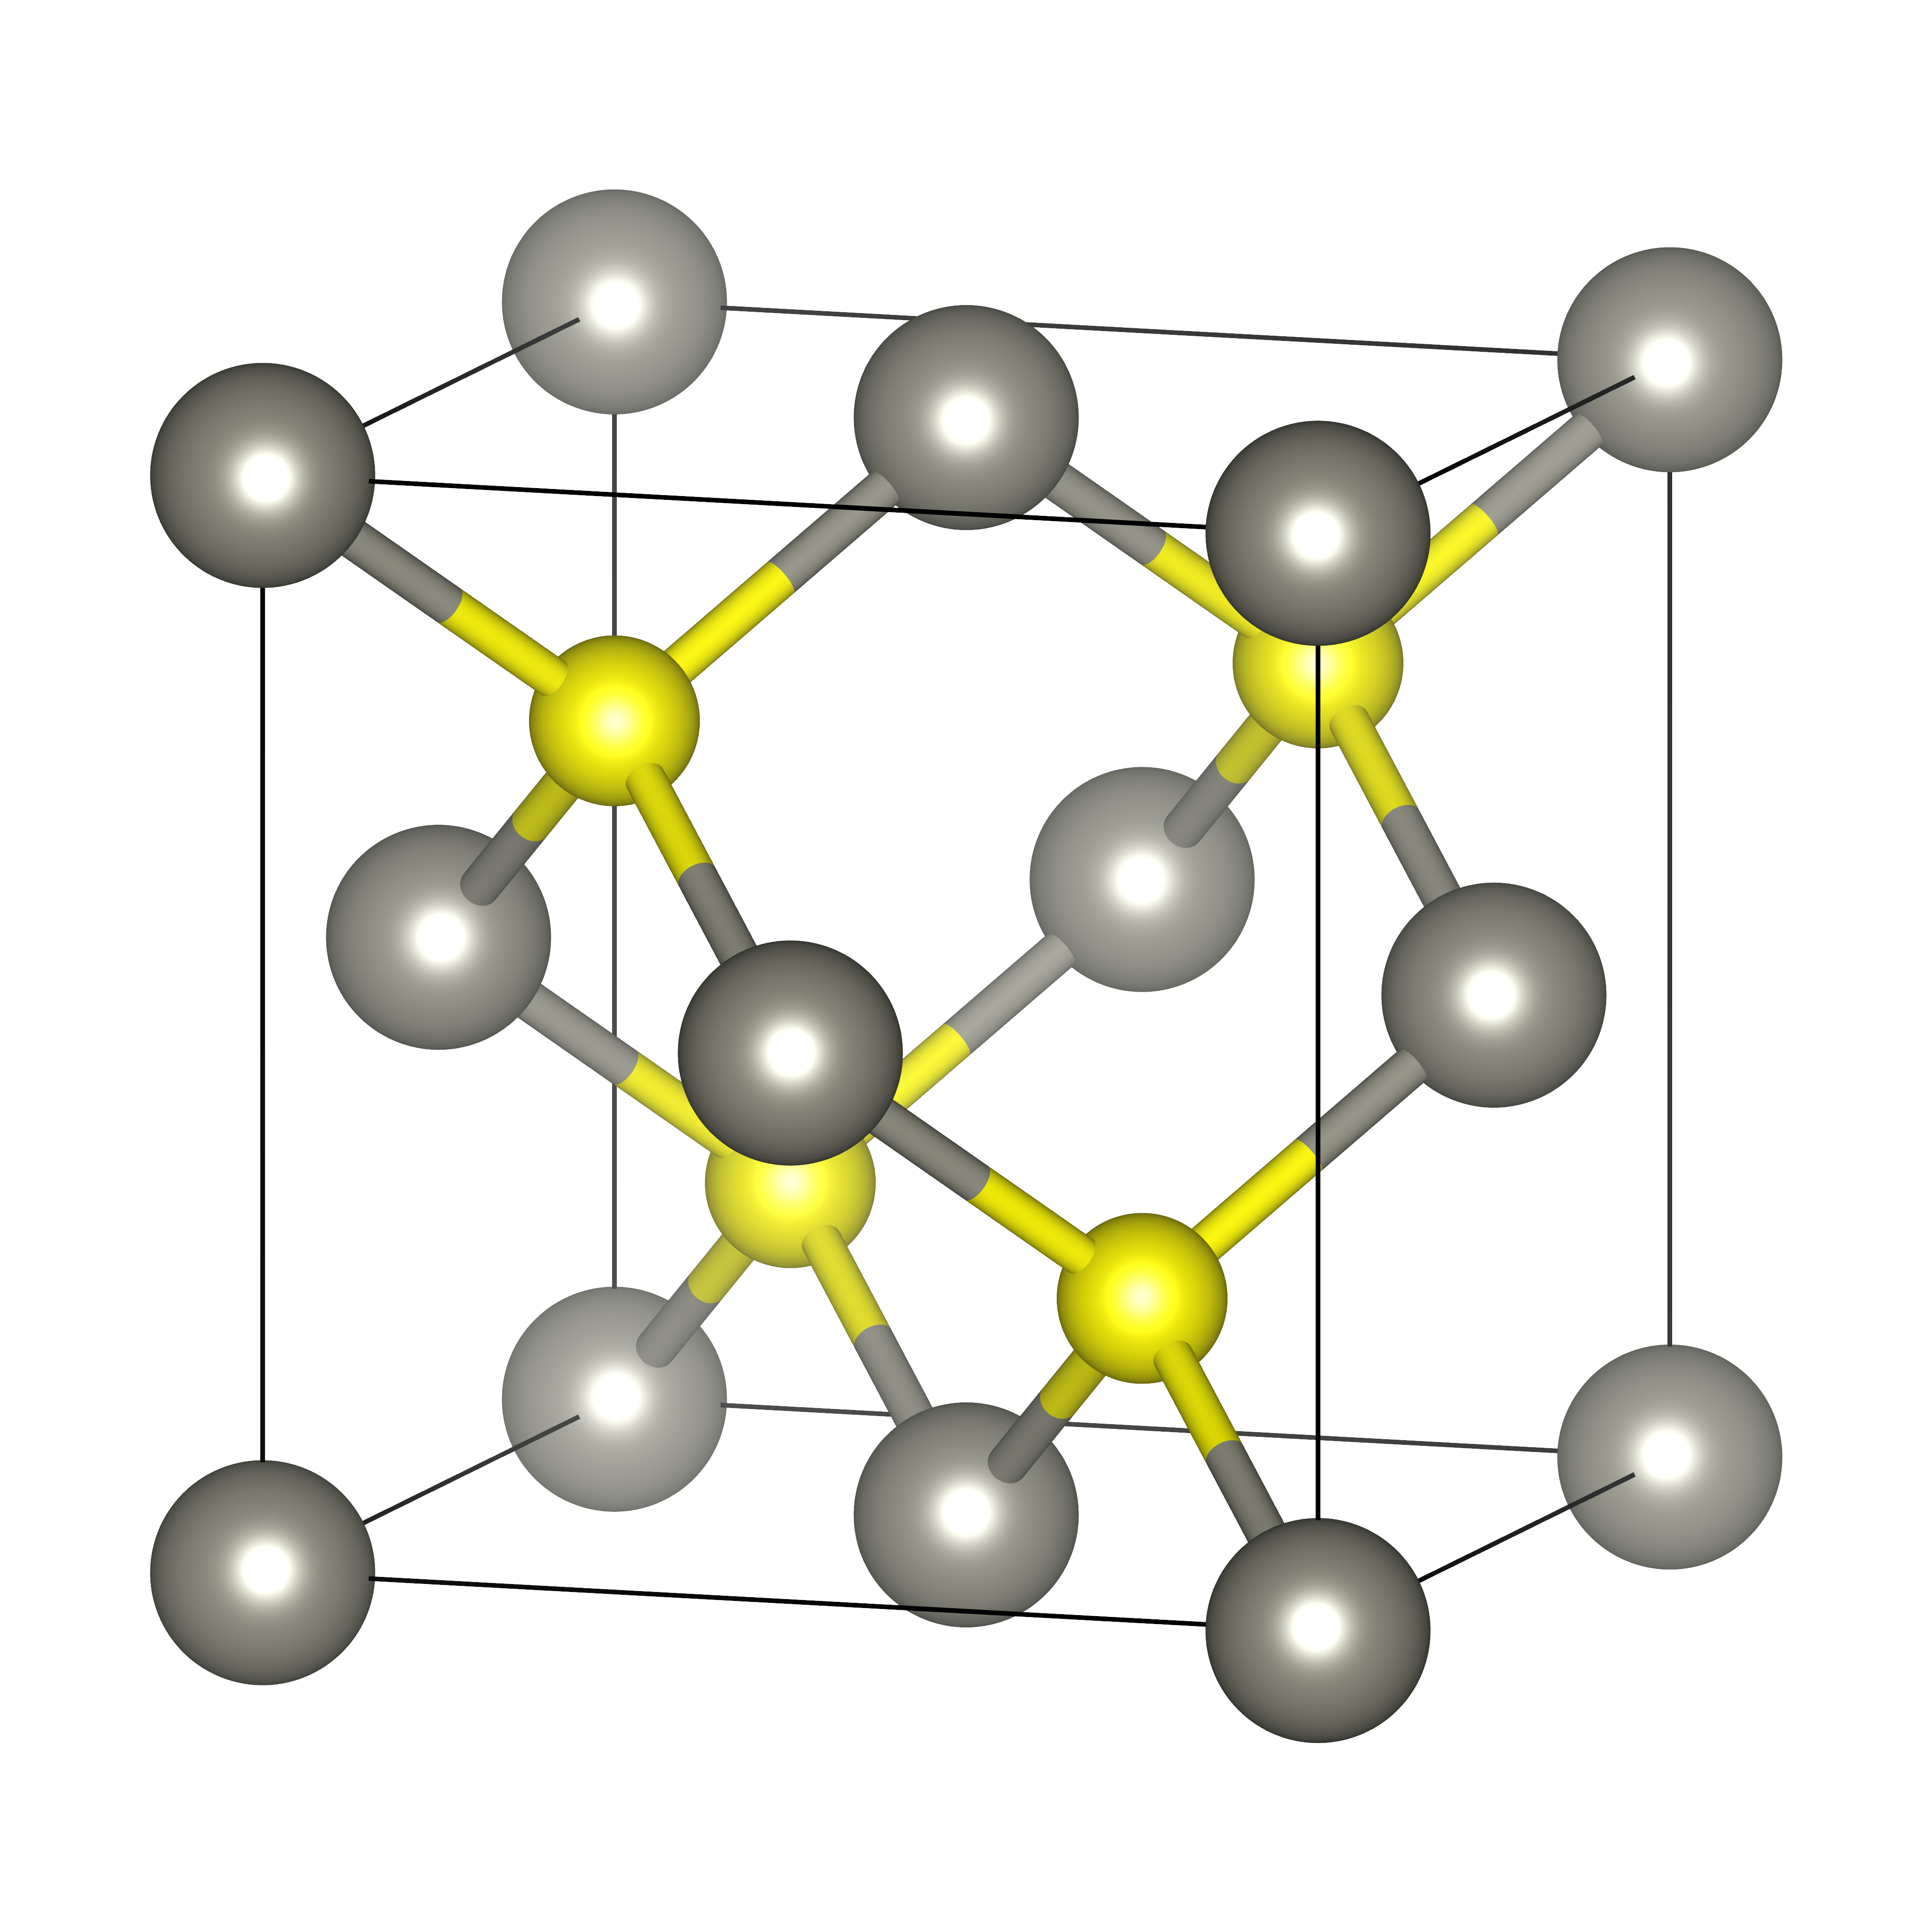
\includegraphics[scale=0.04]{Ch10/Cubic/ZnS_1}
	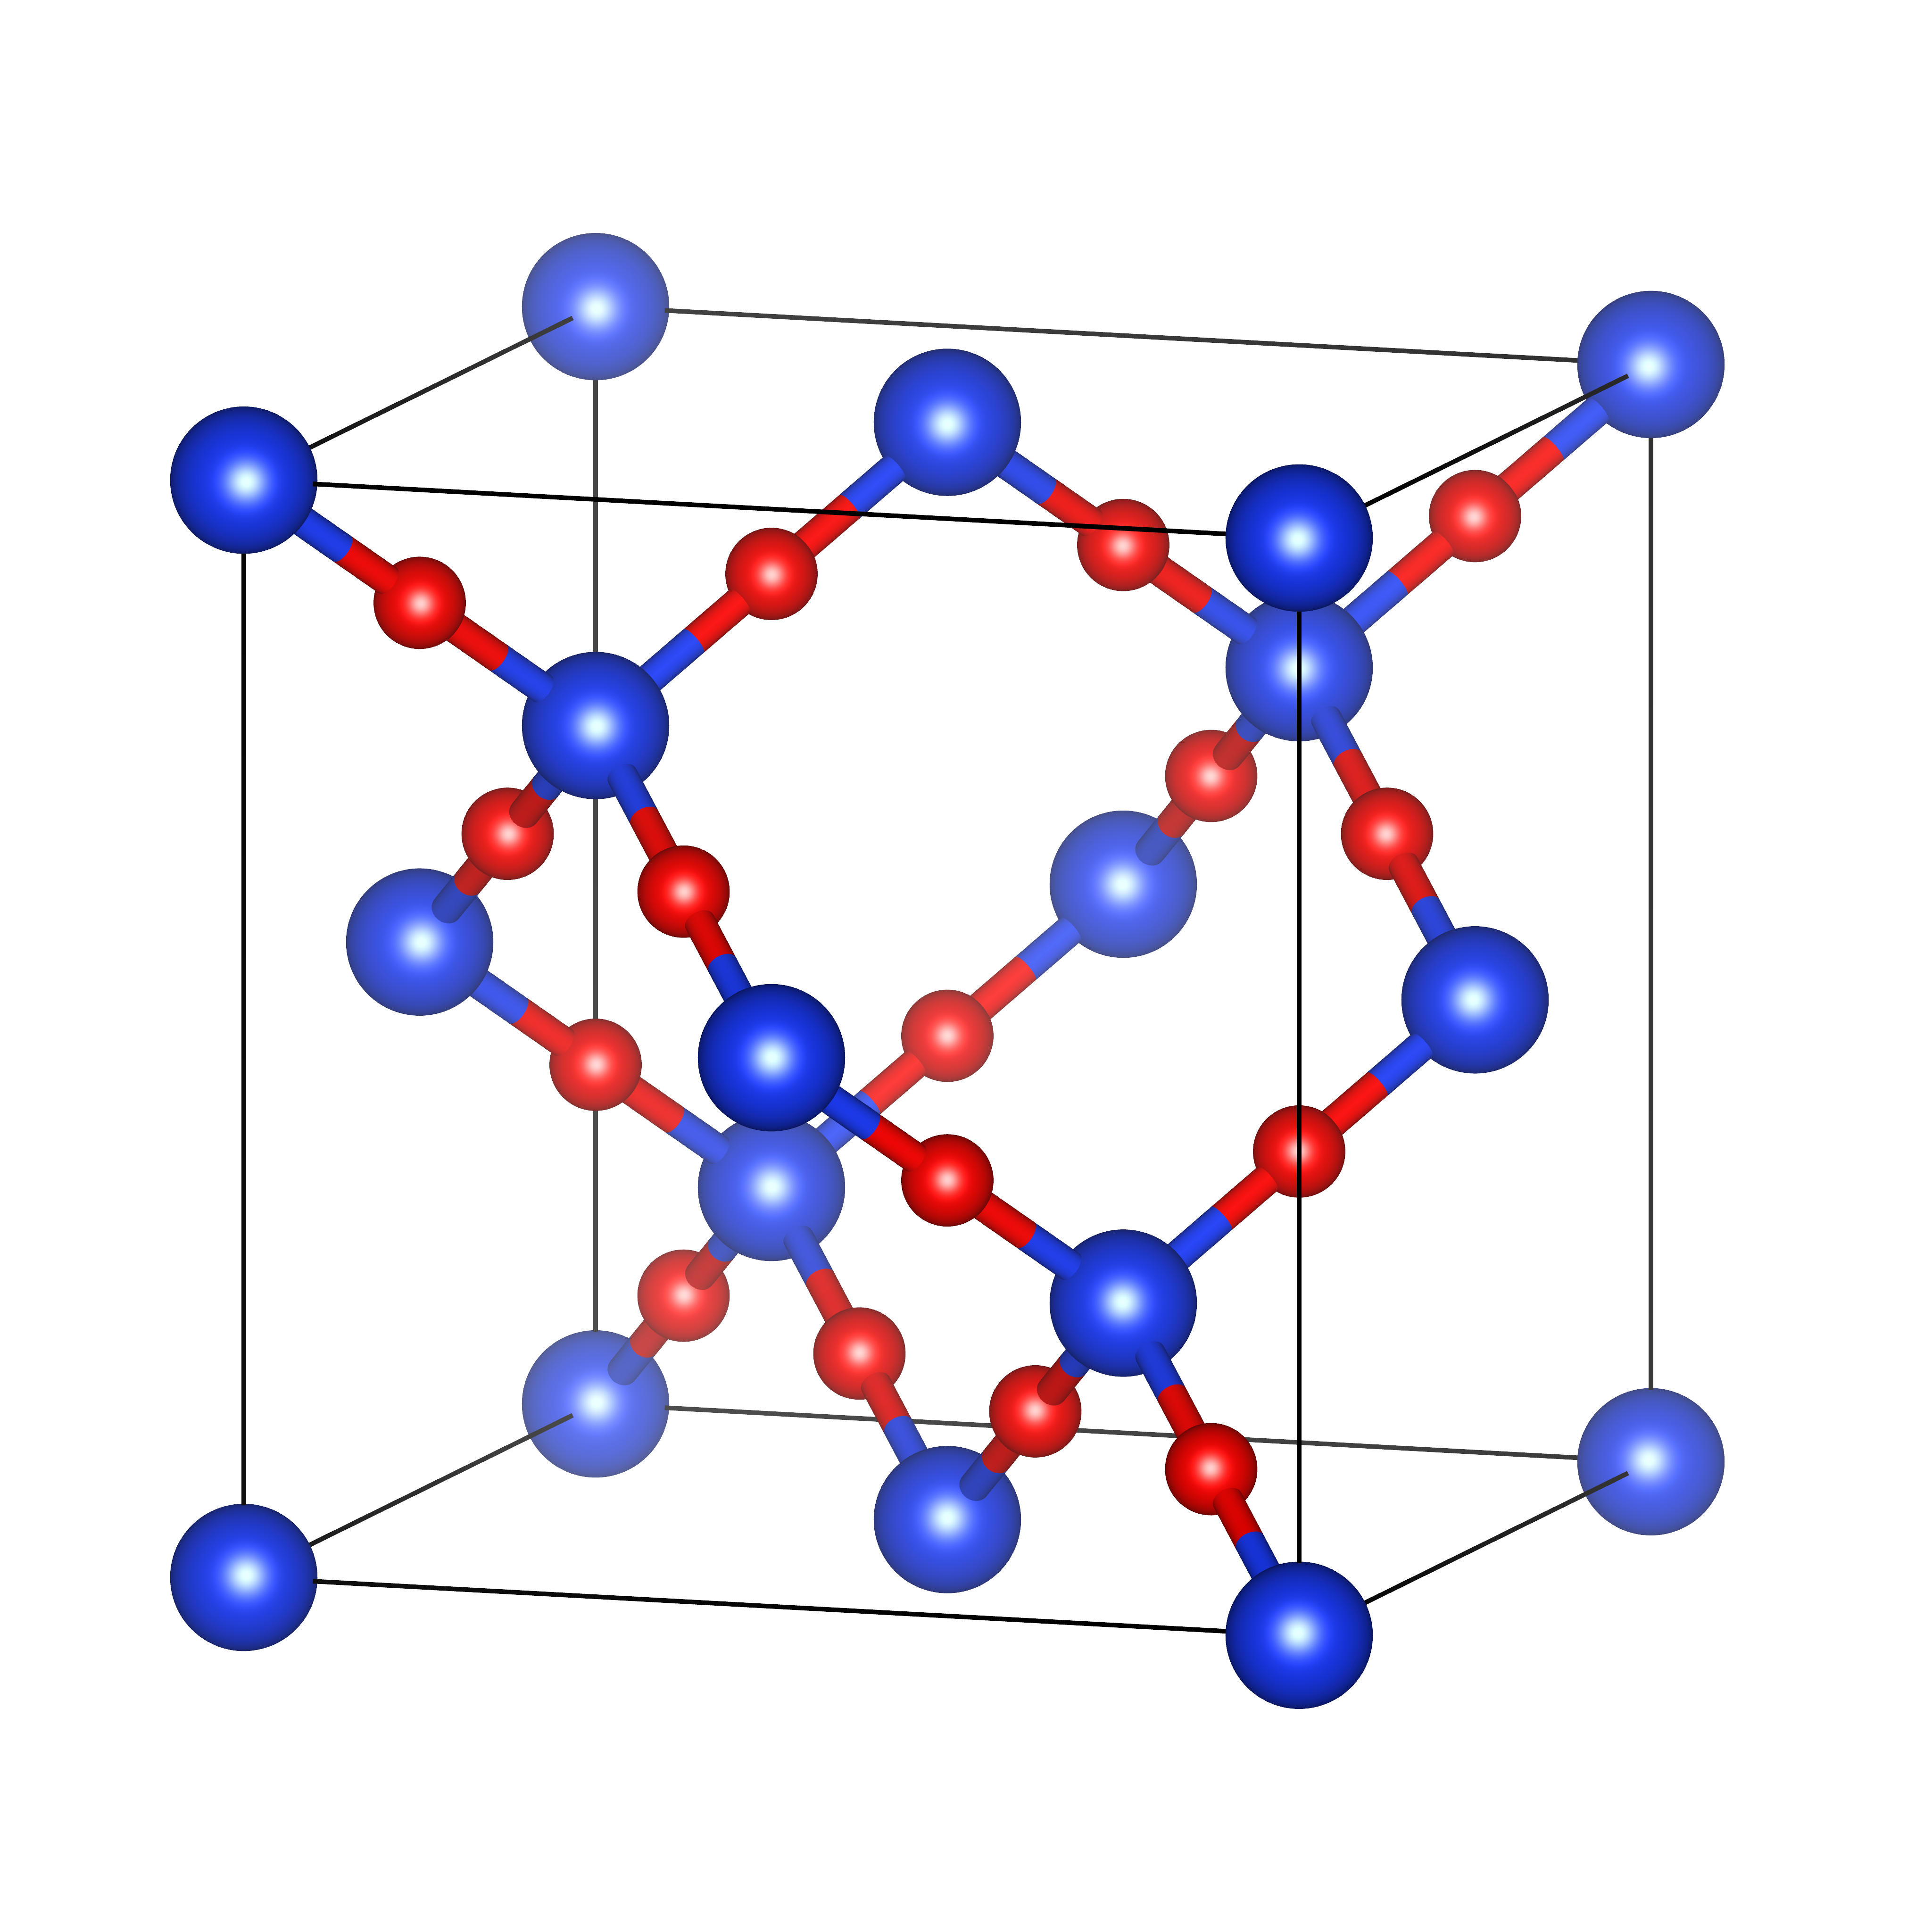
\includegraphics[scale=0.04]{Ch10/Cubic/SiO2}
	\caption{Unit cells of (a) Wurtzite, (b) Sphalerite, (c) $\rm SiO_2$}
	\label{sphalerite}
\end{figure}\\
%
For fluorites $\rm MX_2$, the polyhedron carved out by bonds and lattice planes $\{110\}$ is named rhombohedral dodecahedron.
Its can also be described as M atoms filling half of the cubic sites
in simple cubic packing of X by a tetrahedral pattern, 
i.e. removing half of Cl from CsCl structure, resemblings prussian blue structure $\rm KNiFe(CN)_6$ (see \ref{cscls}).
Note that anti-fluorite structure also exist whose chemical formula take the form of $\rm M_2X$.
These structures are illustrated in figure \ref{fluorite}.\\
%
\begin{figure}[h]
	\centering
	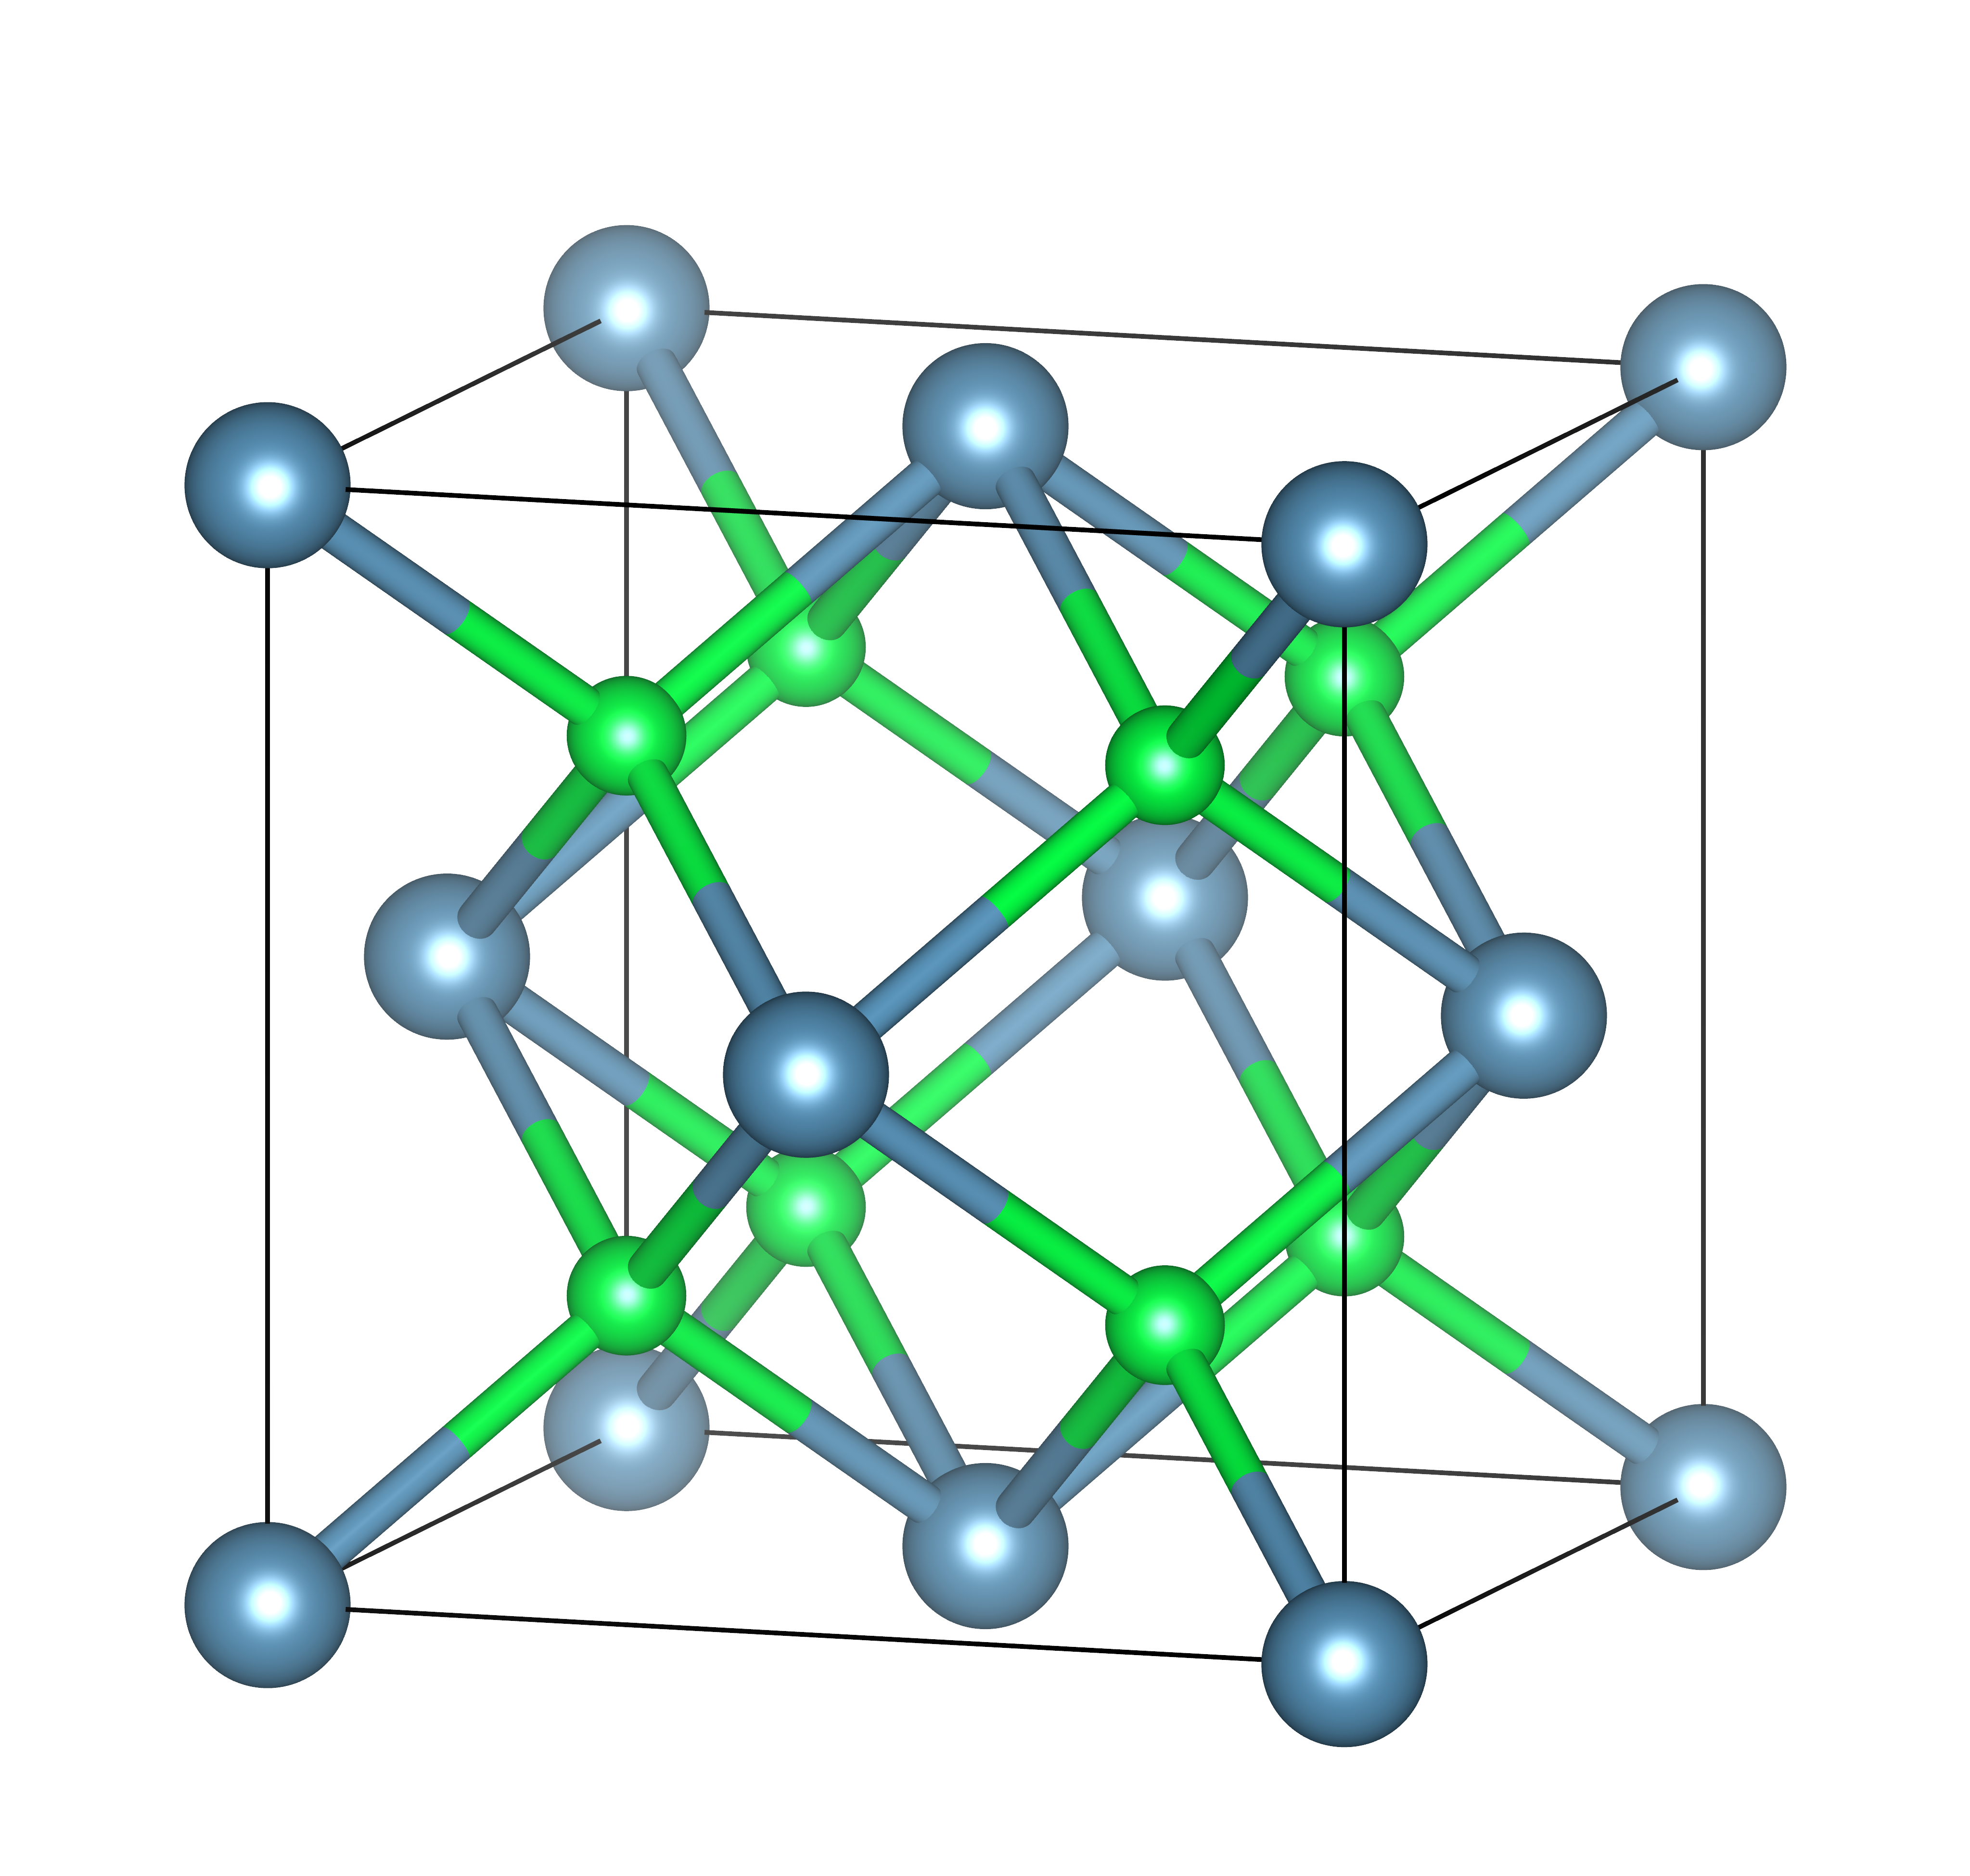
\includegraphics[scale=0.04]{Ch10/Cubic/CaF2}
	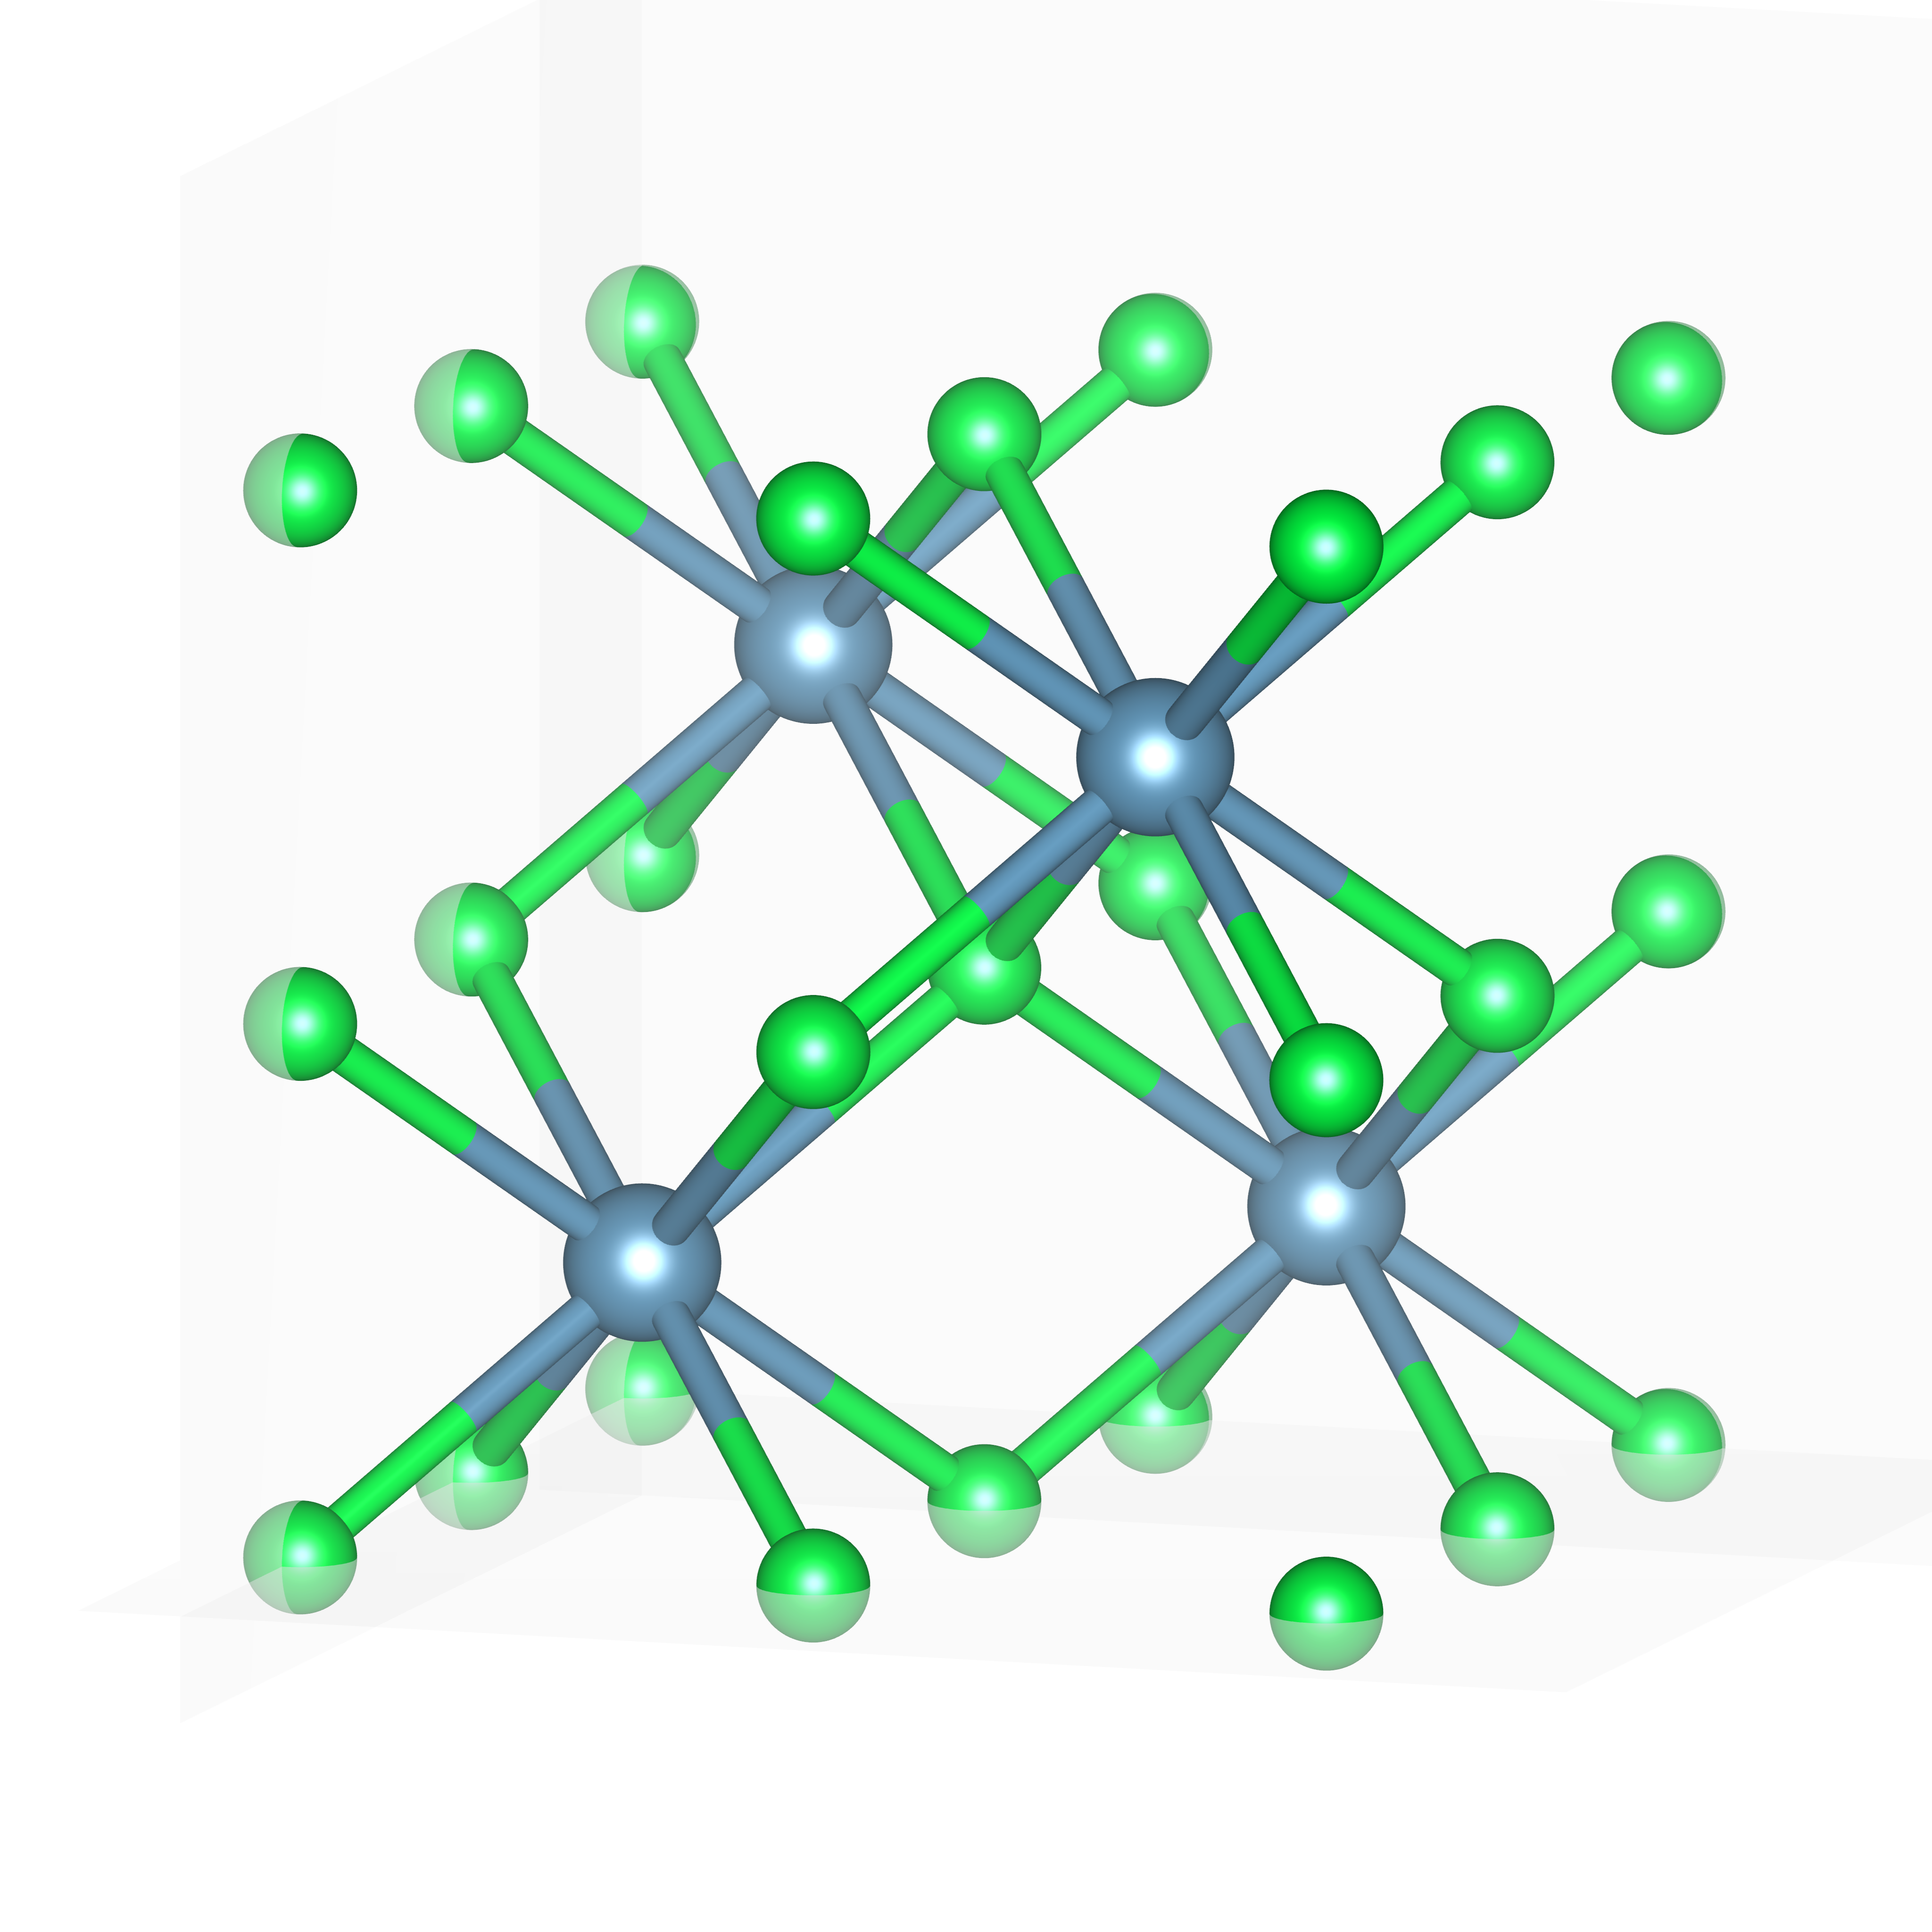
\includegraphics[scale=0.04]{Ch10/Cubic/CaF2_2}
	\caption{Unit cells of fluorites}
	\label{fluorite}
\end{figure}\ \\
%
\section{Lattice Energy}
%
The lattice energy is defined as the enthalpy change of the process where ionic solids turn into free gaseous ions.
It is the energy required to break ionic bonds.
%
\subsection{Born-Mayer Equation}
%
This equation is based on a pure electrostatic model. 
Consider a compound AB with halite structure with one A atom at the center of its cell.
Let $r = r_\text{A}+r_\text{B}$ be the internuclear distance and $z$ the absolute value of their charges.
Calculate the total Coulomb potential energy of the central A atom:
%
\begin{itemize}
	\item Its closest neighbors are the six B's at face-centers with attractive interaction, $V<0$: 
	\[
		V_1 = -\frac{z^2e^2}{4\pi\epsilon_0}\cdot\frac{6}{r}
	\]
	\item Its second closest neighbors are the 12 A's at edge midpoints with repulsive interaction, $V>0$:
	\[
		V_2 = +\frac{z^2e^2}{4\pi\epsilon_0}\cdot\frac{12}{\sqrt{2}r}
	\]
	\item Its third closest neighbors are the 8 B's at vertices with attractive interaction, $V<0$:
	\[
		V_3 = -\frac{z^2e^2}{4\pi\epsilon_0}\cdot\frac{8}{\sqrt{3}r}
	\]
	\item $\cdots$
\end{itemize}
%
Therefore the total electrostatic potential energy for 1 mol A is:
%
\[
	V_n = -\frac{N_Az^2e^2}{4\pi\epsilon_0}
	\left( \frac{6}{\sqrt{1}} - \frac{12}{\sqrt{2}} + \frac{8}{\sqrt{3}} - \frac{6}{\sqrt{4}} + \frac{24}{\sqrt{5}} -\cdots \right)
\]
%
The series in the parentheses will converge into a value unique for every lattice structure, its Madelung constant.
The Madelung constant for some lattice structures are listed in table \ref{madelung}.
%
\begin{table}
	\centering
	\begin{tabular}{@{}lllllll@{}}
		\toprule
		\ \textbf{Lattice Structure}	&	Halite	&	CsCl	&	Fluorite	&	Sphalerite	&	Wurtzite	&	Rutile	\ \\
		\midrule
		\ $A$							&	1.7476	&	1.7677	&	2.5194		&	1.6381		&	1.6413		&	2.408	\ \\
		\bottomrule
	\end{tabular}
	\caption{Madelung constants of several lattice structures}
	\label{madelung}
\end{table}
%
However the atoms are not hard spheres. Their electrons stretch out as wavefunctions, decaying exponentially with distance.
Taking this effect into account, we write the eletron-electron repulsion as:
%
\[
	V_e = N_AC\cdot e^{-r/r^*}
\]
%
where $C$ and $r^*$ are undetermined constants, but they promise a minimal energy at internuclear distance $r$.
By letting the derivative of total energy with respect to internuclear distance zero, we can find $C$ in terms of $r^*$.
After clean-up, we obtain Born-Mayer equation:
%
\[
	\Delta_LH_m = \frac{N_Az^2e^2}{4\pi\epsilon_0r}
	\left(1-\frac{r^*}{r}\right)A
\]
%
where $A$ is its corresponding Madelung constant and $r^*$ takes an empirical value of 34.5 pm.
%
\subsection{Born-Land\'e Equation and Kapustinskii Equation}
%
There're other ways to approximate electron-electron repulsion. 
If we assume the electron cloud of ions with the same noble core stretches as far, 
and use inverse powers to calculate this interaction:
%
\[
	V_e = N_AB\cdot r^{-n}
\]
%
where $n$ depends on the noble core, listed in table \ref{lande}. 
If two ions have different $n$, their arthmetic average is then used.
%
\begin{table}
	\centering
	\begin{tabular}{@{}llllll@{}}
		\toprule
		\ \textbf{Core}	&	He	&	Ne 	&	Ar	&	Kr	&	Xe 	\ \\
		\midrule
		\ $n$			&	5	&	7	&	9	&	10	&	12	\ \\
		\bottomrule
	\end{tabular}
	\caption{Exponent $n$ in Born-Land\'e equation}
	\label{lande}
\end{table}
%
Similar to Born-Mayer equation, $B$ can be determined by differentiating $V$. The result is then:
%
\[
	\Delta_LH_m = \frac{N_Az^2e^2}{4\pi\epsilon_0r}
	\left(1-\frac{1}{n}\right)A
\]
%
which is named Born-Land\'e equation.\\ \\
%
From these two equations, Kapustinskii discovered that 
the ratio of Madelung constants and total stoichiometry of ions in each lattice type only varies slightly, 
and madelung constant increases with coordination number, implying that $A/(\nu r)$ is nearly a constant.\\ \\
%
Therefore, every lattice structure has its degenerate halite structure. 
With this principle at hand, we can use Kapustinskii eqaution for lattice energies:
%
\[
	\Delta_LH_m = \frac{k\nu z^2}{r}\left(1-\frac{r^*}{r}\right)
\]
where $\nu$ is the total formula stoichiometry and $k=1.21\cdot10^5$ $\rm kJ\cdot pm\cdot mol^{-1}$.\\ \\
%
The limitations of these equations are obvious: 
they are still semi-empirical, and covalent bonding interaction are dismissed. 
They only give good results for strong ionic compounds with $\Delta\chi >2$.
%
\subsection{Consequences of Lattice Enthalpies}
%
The key of the former equations is:
%
\[
	\Delta_LH_m \propto \frac{|z_Az_B|}{r_A+r_B}
\]
%
Now we conduct some qualitive analysis.
%
\subsubsection{Thermal Stability}
%
Consider the process of ion decomposition, the size of the ion will surely shrink after the process.
We put aside entropy effects.
If the main product remains solid, the enthalpy change of decomposition is then: 
(Bear in mind that lattice enthalpy is positive. It is the energy absorbed to break lattice.)
%
\[
	\Delta_rH = \Delta_{\text{decomp}}H + \Delta_LH_i - \Delta_LH_f
\]
%
$\Delta_{\text{decomp}}H$ is usually large and positive, 
but as the radius of one ion decreased after decomposition, 
$\Delta_LH_i - \Delta_LH_f <0$ drives the reaction forward.\\ \\
%
For a certain amount of radius decrease, if its counterion is sufficiently large, 
the radius change only reflects in a small amount of reciprocal internuclear distance change.
From the perspective of maths (absolute values are taken):
%
\[ 
	|\Delta_LH_i - \Delta_LH_f| = 
	\frac{1}{r - \Delta r} - \frac{1}{r}  = 
	\frac{\Delta r}{r(r-\Delta r)} = \frac{4\Delta r}{(2r-\Delta r)^2 - \Delta r^2}
\]
%
As the initial internuclear distance $r$ is for sure larger than $\Delta r$, 
the expression above decrease with increasing $r$. 
And for the same ion to decompose, the larger its counterion, the bigger $r$.
Therefore, the larger the counterion, the harder it is for decomposition to occur:
%
\[\boxed{\text{
	Large\ cation\ stabilizes\ large\ anions
}}\]
and vice versa.
%
\subsubsection{Solubility}
%
Dissolving a coumpound in water releases hydration enthalpy at the cost of lattice enthalpy. 
In hydration step, each ion interact with solvent individually, 
so hydration enthalpy is inverse proportional to the radii of individual ions:
%
\[
	\Delta_{\text{solv}}H = \Delta_LH - \sum\Delta_{\text{hyd}}H \propto \frac{1}{r_-+r_+} - \frac{1}{r_-} - \frac{1}{r_+}
\]
Only if one in $r_-,r_+$ is small and the other is big can $\Delta_{\text{solv}}H$ achieve a large negative value 
and hence favours dissolving.
%
\[\boxed{\text{
	Large\ cation\ precipitates\ large\ anions
}}\]
and vice versa.


\section{Crystal Defects and Non-Stoichiometry}
%
Real crystals are imperfect. A defect forms at the cost of lattice enthalpy but gain entropy as a tradeoff. 
At any $T>0$, the Gibbs free energy is minimized by a finite equilibrium defect concentration, 
increasing with increasing temperature until its melting point.
%
\subsection{Intrinsic Point Defects}
%
\begin{itemize}
    \item Schottky defect: A pair of cation and anion vacancies (charge-neutral) appears, 
    		most common in close-packed ionic crystals with high coordination numbers.
    \item Frenkel defect: An ion is displaced from its lattice site into an interstitial position. 
    		Favoured in structures with low coordination and open channels (e.g., AgCl, ZnS).
    \item Exchange defect: Two atoms swap positions; common in alloys and compounds with similar cations 
    		(e.g., AuCu alloy).
\end{itemize}

\subsection{Extrinsic Defects and Doping}

Impurities introduced deliberately dopants create extrinsic defects.
In ionic crystals, aliovalent doping can generate vacancies. For example, Ca$^{2+}$ doped into ZrO$_2$ creates O$^{2-}$ vacancies to maintain charge neutrality, yielding an oxygen-ion conductor.

\subsection{Non-Stoichiometric Compounds}

Some solids exhibit a composition range while retaining the same structure type (e.g., Fe$_{1-x}$O, $0.04\le x\le 0.11$ at 1000$^\circ$C). This requires variable oxidation states of the metal and is common among transition-metal oxides/chalcogenides.

%
\section{Electric Properties of Solids}
%
For a solid to conduct electric currents, it has to have a charge carrier. 
Some crystals have vacancies and ions with small radii so that those ions can migrate from its place to one of the vacancies, conducting current.
But it is more commonly seen that it is the electrons that serve as charge carriers.
This kind of conductor can further be classified by the temperature dependence of its conductivity:
\begin{itemize}
    \item Metallic Conductor: Conductivity decreases with increasing $T$.
    \item Semiconductor \& Insulator: Conductivity increases with $T$.
\end{itemize}
%
\subsection{Tight-Binding Theory and Energy Bands}\label{band}
%
When $N$ identical orbitals interact in an array, the molecular orbital can be solved by secular determinants as in \ref{linear}.
For a one dimentional chain, the result obtained via H\"uckel approximation is:
%
\[
	E_k = \alpha + 2\beta\cos\left(\frac{k\pi}{N+1}\right), \qquad k=1,2,\dots,N.
\]
%
When $N\to+\infty$, the energy difference between adjacent energy levels approaches infinitesimal, 
i.e. the energy levels become a continuous band of width $4|\beta|$. Let
%
\[
	m = \frac{k\pi}{N+1}\,\in\,(0,\pi)
\]
%
The density of states is then:
%
\[
	\rho=\frac{N}{\pi}\left|\frac{\df m}{\df E}\right|=\frac{N}{\pi\sqrt{4\beta^2-(E-\alpha)^2}}
\]
%
Which is a bit counterintuitive that $\rho$ attains minimum at $E=\alpha$ where most states seem to reside.\\ \\
%
Different orbitals form different bands. Some basic definitions are listed:
%
\begin{itemize}
    \item Valence band: The highest band filled with electrons at $T=0$.
    \item Conduction band: The lowest empty band at $T=0$.
    \item Band gap: The energy separation between valence band and conduction band.
    \item Fermi level: The energy of the highest occupied orbital at $T=0$.
\end{itemize}
%
Those are illustrated in figure \ref{band1}
%
\begin{figure}[h]
	\centering 
	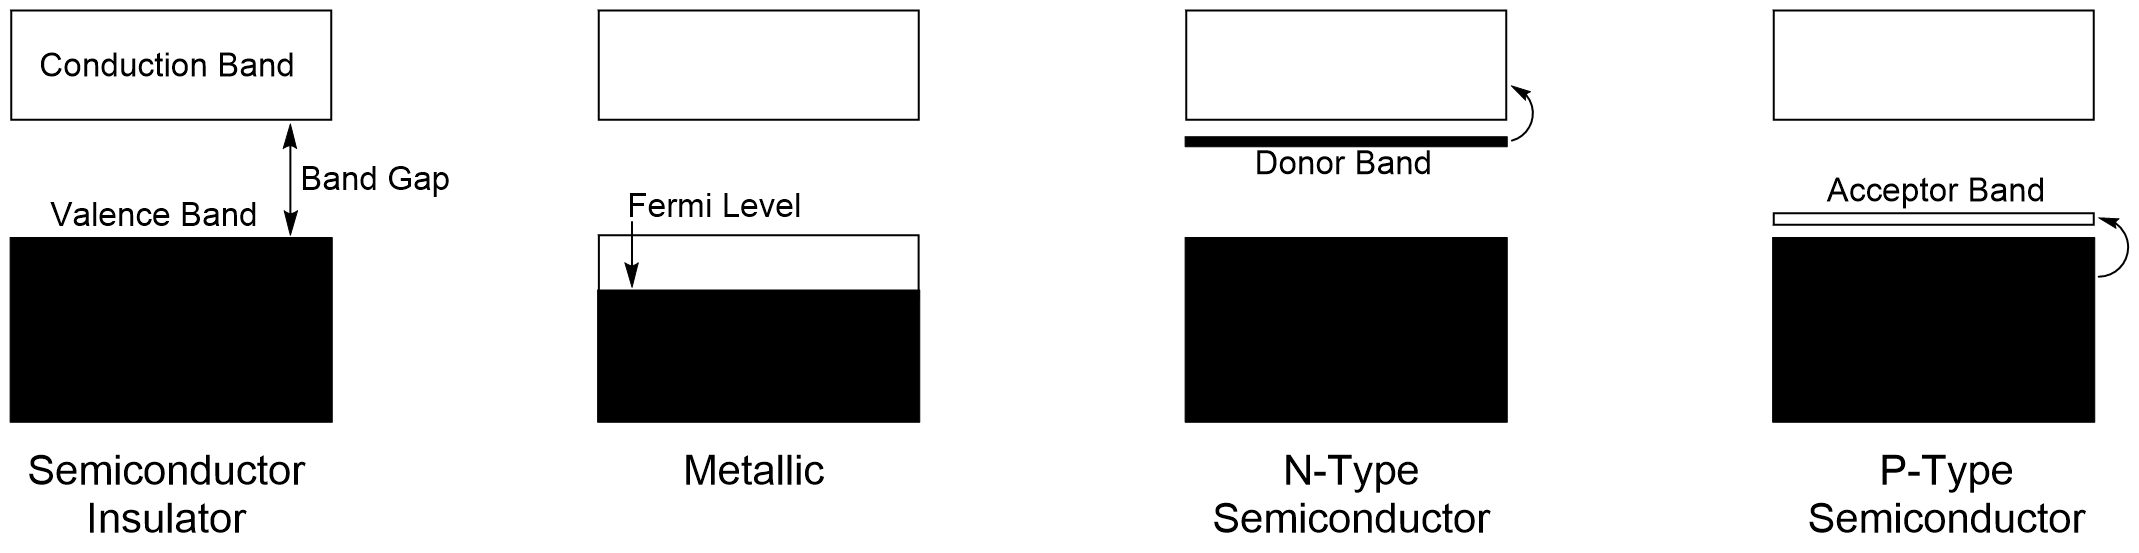
\includegraphics[scale=0.22]{Ch10/Lattice/band}
	\caption{Band structure in crystalline solids}
	\label{band1}
\end{figure}
%
\subsection{Classification by Band Structure}
%
\subsubsection{Metals and Semimetals}
%
In metals, a band is partially filled, or a filled band overlaps with an empty band where electrons are readily excited into nearby empty states. 
As temperature rises the nuclei vibrates more vigorously, scattering electrons' directional motion and thus decreasing conductivity.\\ \\
%
When a filled band just touches an empty band at a few points with zero density of states at contact, 
these compound with weak conductivity as graphite are named semimetals.
%
\subsubsection{Semiconductors and Insulators}
In a semiconductor, a small gap $\Delta E\approx 0.1-3$ eV separates a full valence band from an empty conduction band. 
Thermal excitation follows Boltzmann distribution and therefore conductivity increase with increasing temperature:
\[
    \sigma = \sigma_0 \exp\left(-\frac{\Delta E}{2kT}\right).
\]
where the activation energy is half the band gap width 
as an input energy of $\Delta E$ excites both an electron and a vacancy, but only accounts for one charge carrier.
Whereas for an insulator a large gap $\Delta E \gtrsim 5$ eV prevents thermal excitation at ordinary temperatures.
%
\subsection{Extrinsic and Intrinsic Semiconductors}
%
\subsubsection{N and P-Type Semiconductors}
When group 13 elements are doped into silicon crystals, vacant orbitals are introduced, 
which then form an accrptor band just above the valence band. 
Electrons from the valence band can be thermally excited into these acceptor levels, 
leaving mobile holes in the valence band which exhibits positive charge.
This kind of semiconductors is called p-type semiconductors.\\ \\
%
When group 15 elements get doped into Si, filled levels of electrons are introduced just below the conduction band 
due to extra electrons brought by dopants. Electrons are readily promoted into the conduction band.
This kind of semiconductors is called n-type semiconductors.
%
\subsection{Non-Stoichiometric Semiconductors in Metal Oxides}
%
Transition-metal oxides (and some halides) often exhibit semiconductivity 
due to non-stoichiometry brought by their diverse available valences.
%
\begin{itemize}
    \item N-Type: For high-valent metal-rich oxides, those metal centers are partially reduced so that they contain donor levels, and
    \item P-Type: For low-valent metal-deficient oxides, metal centers are partially oxidized or lost so they have acceptor levels.
\end{itemize}
%
Some examples of n and p-type oxide semiconductors are listed in table \ref{semi}.
%
\begin{table}
	\centering
	\begin{tabular}{@{}ll@{}}
		\toprule
		\ \textbf{Type}		&	\textbf{Examples}					\ \\
		\midrule
		\ N-Type			&	$\rm TiO_2,\ Fe_2O_3,\ ZnO$	\ \\
		\ P-Type			&	$\rm Cr_2O_3,\ MnO,\ FeO,\ CuI$		\ \\
		\bottomrule
	\end{tabular}
	\caption{Examples of intrinsic semiconductors}
	\label{semi}
\end{table}


